%\documentclass{brownthesis}
\documentclass[final,nofigures,notables]{brownthesis}
\usepackage{lmodern}
\usepackage[T1]{fontenc} 
\usepackage{textcomp}
\usepackage[utf8x]{inputenc}
\usepackage[ruled,linesnumbered]{algorithm2e}
\usepackage{amsfonts}
\usepackage{amsmath}
\usepackage{amssymb}
\usepackage{amsthm}
\usepackage{bigstrut}
\usepackage{booktabs}
\usepackage{caption}
\usepackage{ctable} % TODO TO REMOVE
\usepackage{dsfont}
\usepackage{float}
\usepackage{graphicx}
\usepackage{hyperref}
\usepackage{mathtools}
\usepackage{multirow}
\usepackage[sort,compress,numbers]{natbib}
\usepackage{multirow}
\usepackage{setspace}
\usepackage{subfig}
%\usepackage{subfigure} % TODO UNDERSTAND WHICH ONE TO USE
\usepackage{url}
\usepackage{verbatim}
\usepackage{xspace}

\usepackage[show]{notes-alt}

\newcommand{\Sam}{{\cal S}}
\newcommand{\Ds}{{\cal D}}
\newcommand{\Db}{{\cal D}}
\newcommand{\Tab}{{\cal T}}
\newcommand\Itm{{\cal I}}
\newcommand\TOPK{\mathsf{TOPK}}
\newcommand\FI{\mathsf{FI}}
\newcommand\TFI{\mathsf{TFI}}
\newcommand\AR{\mathsf{AR}}
\newcommand\VC{\mathsf{VC}}
\newcommand\EVC{\mathsf{EVC}}
\newcommand{\PARMM}{PARMA\xspace}
\newcommand\prob{\pi}
\newcommand\tfreq{t_\prob}
\newcommand\range{\mathcal{R}}
\newcommand\eb{\mathsf{eb}}
%\newcommand\b{\mathsf{b}}
\newcommand\betw{\mathsf{b}}
\newcommand\kboundbetw{\mathsf{bb}}
\newcommand\kpathbetw{\mathsf{pb}}
\newcommand\VD{\mathsf{VD}}
\newcommand\expectation{\mathbb{E}}
\newcommand\var{\mathrm{Var}}
\newcommand\mse{\mathrm{MSE}}

\newif\ifproof
\prooftrue

\DeclareMathOperator{\op}{op}
\DeclareMathOperator{\eqop}{eqop}
\DeclareMathOperator{\bool}{bool}

\newtheorem{corollary}{Corollary}
\newtheorem{lemma}{Lemma}
\newtheorem{theorem}{Theorem}
\newtheorem{fact}{Fact}
\newtheorem{claim}{Claim}

\theoremstyle{definition}
\newtheorem{definition}{Definition}


\begin{document}
\doublespacing
\pagenumbering{alph} % hack to suppress hyperref errors

\submitdate{May 2014}
\title{Sampling-based Randomized Algorithms for Big Data Analytics}
\author{Matteo Riondato}
\degrees{Laurea, Universit\`a di Padova, Italy, 2007\\
Laurea Specialistica, Universit\`a di Padova, Italy, 2009\\
Sc.~M., Brown University, 2010}
\principaladvisor{Eli Upfal}
\reader{U\u gur \c Cetintemel}
\reader[(Applied Mathematics)]{Basilis Gidas}
\dean{Peter M.~Weber}
\begin{abstract}
  %Thanks to technology advancements, data are nowadays being collected for
  %almost all human activities and many natural phenomena, to the point that the
  %challenge in many disciplines is the \emph{analysis} of data rather than the
  %collection of it. 
  The huge volume, high variety of origins and formats, and
  ever-increasing velocity requested when reporting results, make the
  task of analyzing the data a complex computational problem known as \emph{Big
  Data Analytics}. Traditional techniques developed in statistics are often
  insufficient, lacking scalability (\emph{volume}), speed (\emph{velocity}), or
  applicability (\emph{variety}). The thesis of this work is that it is possible
  to address these issues by using modern techniques from \emph{statistical learning
  theory} to develop and analyze of efficient randomized algorithms for
  extracting collections of interesting patterns from large transactional
  datasets and huge graphs. Problems of interest include frequent itemsets and
  association rules mining, frequent subgraphs extraction, and database queries
  selectivity estimation. The two main lines of research involve exploiting the
  trade-off between \emph{speed} and \emph{accuracy} by developing algorithms
  that only analyze small random samples of the original data, and assessing the
  \emph{statistical significance} of the extracted patterns by creating
  statistical tests that can be applied in a multiple hypothesis testing
  setting. The analysis of the algorithms uses tools from statistical learning
  theory like \emph{VC-dimension}, \emph{shatter coefficients}, and
  \emph{Rademacher averages}. A byproduct of this thesis is the evidence that
  these tools, often considered only of theoretical interest, can be of great
  use in practice. For each proposed algorithm, an extensive empirical
  evaluation assess its performances on real and artificial benchmark datasets,
  showing that their output is often of quality higher than what the theoretical
  analysis could guarantee.
\end{abstract}

\abstractpage
%\abstractpage
\beforepreface
%\prefacesection{Vita}
%   It all started in a little log cabin ...
%\prefacesection{Preface}
%   This thesis tells you all you need to know about...
\prefacesection{Preface}
\iffalse
This dissertation is the work of many people who may have not realize how much
they were helping.

I am deply indebted to my advisor Eli Upfal. We met in Padova in October 2008
and after two weeks I asked him whether I could come to the States to do my
master thesis. Surprisingly for me, he said yes. Since then he helped me in all
possible ways, even when I seemed to run away from his help (and perhaps I
foolishly was). This dissertation started when he casually suggested
VC-dimension as a tool to overcome some limitations of the ``Chernoff + Union
bound'' technique. After that, Eli was patient to let me find out what it was,
interiorize it, and start using it. He was patient when I kept uing it despite
his suggestions to move on (and I am not done with it yet). He was patient when
it became clear that I no longer knew what I wanted to do after grad school. His
office door was always open for me and I abused of his time and patience. He has
been my mentor and I will always be proud of having been his pupil. I hope he
will be, if not proud, at least not dissatisfied with what I am and will become,
no matter where life leads me.  

U\vg ur \cC etintemel and Basilis Gidas were on on my thesis committee and have
been incredibly valuable in teaching me about databases and statistics
(respectively) and above all in encouraging me when I had doubts about my future
perspectives.

Fabio Vandin was, in my opinion, my older brother in academia. We came to
Providence almost together from Padua and we are leaving it almost together.
Since I first met him, he was the example that I wanted to follow. If Fabio was
my brother, Olya Ohrimenko was my sister at Brown, with all the up and downsides
of being the older sister. I am grateful to her.

Andrea Pietracaprina and Geppino Pucci were my mentors in Padua and beyond. I
would be ungrateful if I forgot to thank them for all the help, the support, the
encouragement, and the frank conversations that we had on both sides of the
ocean.

Aris Anagnostopoulos and Luca Becchetti hosted me in Rome when I visited
Sapienza in Summer 2011. They taught me more than they probably realize about
doing research. 

Francesco Bonchi was my mentor at Yahoo Labs in Barcelona in the Summer 2012. He
was much more than a boss or a supervisor. He was a colleague in research, a
fussball fierce opponent, a companion of cervezas on the Rabla de Poble Nou.
He shattered a lot of the cancrenous ``certainties'' that I created for myself,
and showed me what it means to be a great researcher and manager.

The Italian gang at Brown was always supportive, encouraging, and provided
moments of fun, food, and festivity: Michela Ronzani, Marco Donato, Cristina
Serverius, Nicole Gerke, Erica Moretti, and many many others. I will cherish the
moments I spent with with them for a long time.

My friends in Italy were always there when I came back and it was like I just
left for a day: Giacomo, Mario, Fabrizio, Nicol\'o, the various Giovanni,
Valeria, Iccio, Matteo, Simone, Elena, and all the others. Let's go to Anfora soon!

Mackenzie has been incredible in the last year and I believe she will be
incredible for years to come. She supported me whenever I had a doubt or changed
my mind. Whenever I was stressed she made me laugh. Whenever I felt lost, she
made me realize that I was following the path. I hope I gave her something,
because she gave me a lot.

Mamma, Pap\`a, and Giulia have been closest to me despite the oceanic distance.
They were the lighthouse and safe harbour in the nights of doubts, and the solid
rock when I was falling, and the warm fire when I was cold. I will come back,
one day.

This dissertation is dedicated to my grandparents Luciana, Maria, Ezio, and
Guido. I wish one day I could be half of what they are and have been.
\fi


\afterpreface

We now extend the results presented in Chapter~\ref{ch:vcmine} and introduce
PARMA, a randomized parallel algorithm for approximate frequent itemset mining,
that makes the problem of Frequent Itemsets and Association Rules mining (FIM)
embarassingly parallel, thus exhibiting near-linear speedup with the number of
machines. PARMA combines random sampling and parallelization techniques in a
novel fashion.  It mines, in parallel, a set of small random samples and then
filters and aggregates the collections of frequent itemsets or association rules
obtained from each sample.  Our work is orthogonal to other approaches, like
PFP~\citep{LiWZZC08}, which focuses on parallelizing the mining phase in order
to decrease the corresponding component of the cost. Due to the use of random
sampling, the output of PARMA is an approximation of
the collection of FIs or ARs in the dataset, but leveraging on the results
presented in
Chapter~\ref{ch:vcmine}, PARMA offers tight probabilistic guarantees on the
quality of the approximated collections returned in output. In particular it
guarantees that the output is an $\varepsilon$-approximation of the real
collection with probability at least $1-\delta$, where $\varepsilon$ and
$\delta$ are parameters specified by the user (see Section~\ref{sec:parmadef} for
formal definitions). 
PARMA is designed on
MapReduce~\citep{DeanG08}, a novel parallel/distributed architecture that has
raised significant interest in the research and industry communities. MapReduce
is capable of handling very large datasets and efficiently executing parallel
algorithms like PARMA.

To our knowledge PARMA is the first algorithm to exploit the combination of
random sampling and parallelization for the task of Association Rules Mining. 

A number of previous works explored either parallel
algorithms~\citep{BuehrerPTKS07,CongHHP05,EHZaiane06,FangEtAl08,LiuLZT07,OzkuralUA11,JinYA05,Zaki99}
or random
sampling (see Sect.~\ref{sec:vcmineprevwork})
for the FIM task, but the two approaches have been seen somewhat orthogonal
until today. In PARMA, the disadvantages of either approach are evened out by
the advantages of the other. In the spirit of \emph{moving computation to the
data} to minimize communication, we avoid data replication, and preserve the
advantages of parallelization by using of multiple independent small random
samples of the dataset which are mined in parallel and have only their results
aggregated. Similarly, we are not subject to the inherent trade-off between the
size of the random sample and the accuracy of the approximation that can be
obtained from it, as PARMA would only have to mine more samples of the same size
in parallel to get higher quality approximations.

Although PARMA is not the first algorithm to use MapReduce to solve the
FIM task, it differs from and enhances previous
works~\citep{CryansRC10,GhotingKPK11,Hammoud11,LiWZZC08,LiZ11,YangLF10,ZhouZCLF10}
in two crucial aspects. First, it significantly reduces the data that is
replicated and transmitted in the \emph{shuffle} phase of MapReduce.  Second,
PARMA is not limited to the extraction of Frequent Itemsets but can also
directly compute the collection of Association Rules in MapReduce. In previous
works, association rules had to be created sequentially after the Frequent
Itemsets had been computed in MapReduce. 

We conducted an extensive experimental evaluation to test the relative
performance, scalability and accuracy of PARMA across a wide range of
parameters and datasets. Our results suggest that PARMA can
significantly outperform exact mining solutions, has
near-linear speedup, and, as data and nodes are scaled together, is
able to achieve near constant runtimes. Also, our accuracy evaluation
shows that PARMA consistently computes approximated collections
of higher quality than what can be analytically guaranteed.

In this chapter:
\begin{enumerate}
\item We present PARMA, the first randomized MapReduce algorithm for discovering
  approximate collections of frequent itemsets or association rules with
  near-linear speedup.
\item We provide analytical guarantees for the quality of the approximate
  results generated by the algorithm.
\item We demonstrate the effectiveness of PARMA on many datasets and compare
  the performance of our implementation to that of several exact FIM algorithms
  on MapReduce.
\end{enumerate}


\chapter{The Vapnik-Chervonenkis Dimension}\label{ch:vcdim}
In this dissertation we explore the use of random sampling to develop fast and
efficient algorithms for data analytics problems. The use of sampling is not new
in this area but previously presented algorithms were severely limited by their
use of classic probability tools like the Chernoff bound, the Hoeffding bound,
and the union bound~\citep{MitzenmacherU05} to derive the sample size
necessary to obtain approximations of (probabilistically) guaranteed quality.
Instead, we show that it is possible to obtain much smaller sample sizes, and
therefore much more efficient algorithms, by using concepts and results from
\emph{statistical learning theory}~\citep{Vapnik99,Vapnik98}, in particular
those involving the \emph{Vapnik-Chervonenkis (VC) dimension} of the problem.

The VC-Dimension was first introduced in a seminal article~\citep{VapnikC71} on
the convergence of probability distributions, but it was only with the work
of~\citet{HausslerW86} and~\citet{BlumerEHW89} that it was applied to the field
of learning. \citet{BoucheronBL05} present a good survey of the field with many
recent advances. Since then, VC-dimension has encountered enormous success and
application in the fields of computational
geometry~\citep{Chazelle00,Matousek02} and machine
learning~\citep{AnthonyB99,DevroyeGL96}. Other applications include database
management and graph algorithms.  In the former, it was used in the context of
constraint databases to compute good approximations of aggregate
operators~\citep{BenediktL02}.  VC-dimension-related results were also recently
applied in the field of database privacy by~\citet{BlumLR08} to show a bound on
the number of queries needed for an attacker to learn a private concept in a
database. \citet{Gross11} showed that content with unbounded VC-dimension can
not be watermarked for privacy purposes. In the graph algorithms literature,
VC-Dimension has been used to develop algorithms to efficiently detect network
failures~\citep{Kleinberg03,KleinbergSS08}, balanced
separators~\citep{FeigeM06}, events in a sensor networks~\citep{GandhiSW10}, and
compute approximations of the shortest paths~\citep{AbrahamDFGW11}.

We outline here only the definitions and results that we use throughout the
dissertation. We refer the reader to the works of~\citet[Sect.~14.4]{AlonS08},
~\citet[Sect.~3]{BoucheronBL05}, \citet[Chap.~4]{Chazelle00},
\citet[Sect.~12.4]{DevroyeGL96}, \citet[Chap.~3]{MohriRT12},
and~\citet{Vapnik99,Vapnik98} for more details on the VC-dimension theory. 

\section{Preliminaries on VC-dimension}
A {\em range space} is a pair $(D,\range)$ where $D$ is a (finite or infinite)
domain and $\range$ is a (finite or infinite) family of subsets of $D$. The
members of $D$ are called {\em points} and those of $R$ are called {\em ranges}.
The Vapnik-Chernovenkis (VC) Dimension of $(D,\range)$ is a measure of the
\emph{complexity} or \emph{expressiveness} of $\range$~\citep{VapnikC71}.
Knowning (an upper bound) to the VC-dimension of a range space can be very
useful: if we define a probability distribution $\nu$ over $D$, then a finite
upper bound to the VC-dimension of $(D,\range)$ implies a bound to the number of
random samples from $\nu$ required to approximate the probability
$\nu(R)=\sum_{r\in R}\nu(r)$ of each range $R$ simultaneously using the
\emph{empirical average} of $\nu(R)$ as estimator. 

Given $A\subset D$, The {\em projection} of $\range$ on $A$ is defined as
$P_\range(A)=\{R\cap A ~:~ R\in\range\}$. If $P_\range(A)=2^A$, then $A$ is said
to be {\em shattered by $\range$}. 

\begin{definition}\label{def:vcdim}
  Given a set $B\subseteq D$, the \emph{empirical Vapnik-Chervonenkis (VC)
  dimension of $\mathcal{R}$ on $B$}, denoted as $\EVC(\range,B)$ is the
  cardinality of the \emph{largest} subset of $B$ that is shattered by $\range$. If
  there are arbitrary large shattered subsets, then $\EVC()=\infty$. The
  \emph{VC-dimension of $(D,\range)$} is defined as
  $\VC\left((D,\range)\right)=\EVC(\range,D)$.
\end{definition}

For any range space, we have that its VC-dimension cannot be greater than
$d=\lfloor\log_2|\range|\rfloor$ since for any $t>d$, one would need $2^t$
ranges to shatter a set of size $t$. 

A range space $(D,\range)$ with an infinite set of points $D$ and
an infinite family of ranges $\range$ can have a \emph{finite} VC-dimension. A simple
example is the family of open intervals in $\mathbb{R}$ (i.e., $D=\mathbb{R}$ and $\range$
contains all the half-closed intervals $[a,+\infty)$ and $(-\infty, a)$ for any
$a\in\mathbb{R}$). Let $A=\{x,y,z\}$ be the set of three points such that
$x<y<z$. There is no interval $R\in\range$ such that $R\cap A=\{x,z\}$ so the
VC-dimension of this range space is less than 3. This result can be generalized
to higher dimensions.  
\begin{lemma}[Lemma 10.3.1~\citep{Matousek02}]\label{lem:matousek} The
  VC-Dimension of the range
  space $(\mathbb{R}^d, \range)$, where $\range$ is the set of all half-spaces
  in $\mathbb{R}^d$ equals $d+1$.
\end{lemma}
Another example of range space and its VC-dimension is shown in Fig.~\ref{fig:rectangles}.

\begin{figure}[ht]
  \centering
  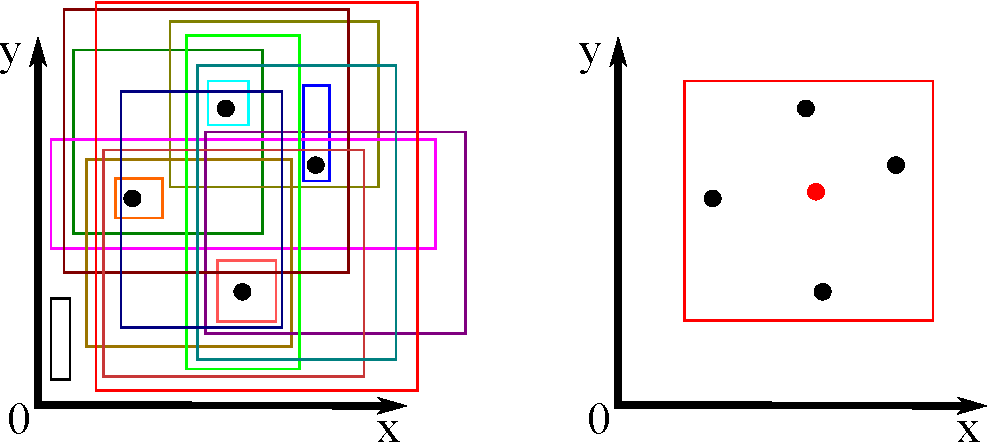
\includegraphics[width=.75\textwidth,keepaspectratio]{prelims/rectangles}
  \caption{Example of range space and VC-dimension. The space of points is the
  plane $\mathbb{R}^2$ and the set $\range$ of ranges is the set of all
  \emph{axis-aligned rectangles}. The figure on the left shows graphically that
  it is possible to shatter a set of four points using 16 rectangles. On the
  right instead, one can see that it is impossible to shatter five points, as,
  for any choice of the five points, there will always be one (the red point in
  the figure) that is internal to the convex hull of the other four, so it would
  be impossible to find an axis-aligned rectangle containing the four points
  but not the internal one. Hence $\VC((\mathbb{R}^2,\range))=4$.}
  \label{fig:rectangles}
\end{figure}

A classic example of a range space with infinite VC-dimension is the space of sine
functions. Let $D=\mathbb{R}^2$ and, for any $\omega\in\mathbb{R}$, let
$A_{\omega}$ be the subset of $\mathbb{R}^2$ that lies \emph{above} the
curve $\sin(\omega t)$, for $t\in \mathbb{R}$. It is possible to
shatter any set $S$ of points by choosing an appropriate $\omega_A$ for each
subset $A\subseteq S$.

Let $\nu$ be a probability distribution on the points of $D$, and let
$X_1^k=(X_1,\dotsc,X_k)$ be a bag of elements from $D$. For any subset
$A\subseteq D$, we define the function 
\[
\nu_{X_1^k}(A)=\frac{1}{k}\sum_{j=1}^k\mathds{1}_A(X_j),\]
where $\mathds{1}_A$ is the indicator function for the set $A$. When $X_1^k$ is
a collection of \emph{independent samples from $\nu$}, then $\nu_{X_1^k}(A)$ is known as the
\emph{empirical average} of $\nu(A)=\sum_{a\in A}\nu(a)$ on $X_1^k$ and is an
\emph{unbiased estimator} for $\nu(A)$ (i.e.,
$\expectation[\nu_{X_1^k}(A)]=\nu(A)$). One of the main applications of
(empirical) VC-dimension is in giving bounds to the number of samples from $\nu$
needed to \emph{simultaneously} approximate the probabilities $\nu(A$) of all
$A\in\range$ using their empirical averages, in the following sense.

\begin{definition}\label{def:eapprox}
  Let $(D,\range)$ be a range space and $\nu$ be a probability distribution on
  $D$. For $\varepsilon\in(0,1)$, an \emph{$\varepsilon$-approximation to
  $(D,\range,\nu)$} is a bag $S$ of elements of $D$ such that 
  \begin{equation}\label{eq:defeapprox}
  \sup_{A\in\range}|\nu(A)-\nu_S(A)|\le\varepsilon\enspace.
\end{equation}
\end{definition}

If $D$ is \emph{finite} and $\nu$ is the \emph{uniform} distribution on $D$, then
$\nu(A)=|A|/|D|$, and~\eqref{eq:defeapprox} is equivalent to
\[
\left|\frac{|A|}{|D|}-\frac{|A\cap S|}{|S|}\right|\le\varepsilon, \forall
A\in\range.
\]
Indeed this will be often but not always the case in later chapters, and we will
simplify the notation by dropping $\nu$ and saying that $S$ is an
$\varepsilon$-approximation to $(D,\range)$.

A great result by~\citet{VapnikC71} showed that it is possible
to compute a $\varepsilon$-approximation with a limited number samples from
$\nu$, provided an upper bound to the VC-dimension of $(D,\range)$ or to its
empirical VC-dimension on a subset of $D$ is known. The original result was
improved multiple times.  Here we present the most recent improvement.

\begin{theorem}[Thm.~2.12~\citep{HarPS11}, see also~\citep{LiLS01}]\label{thm:eapprox}
  Let $(D,\range)$ be a range space with $\VC(\range)\le d$, and let $\nu$ be a
  distribution on $D$. Given $\varepsilon,\delta\in(0,1)$, let
  %and a positive integer $\ell$, let
  \begin{equation}\label{eq:vceapprox}
  %  \varepsilon = \sqrt{\frac{c}{\ell}\left(d + \log\frac{1}{\delta}\right)}
  \ell = \frac{c}{\varepsilon^2}\left(d + \log\frac{1}{\delta}\right)
  \end{equation}
  where $c$ is an universal constant. Then, a bag of $\ell$ elements of $D$
  sampled independently according to $\nu$ is an $\varepsilon$-approximation to
  $(\range,\nu)$ with probability at least $1-\delta$.
\end{theorem}
The constant $c$ is approximately $0.5$ and it is
\emph{universal}, i.e., it does not depend on any parameter~\citep{LofflerP09}.  
It is also interesting to note that, if $|D|$ is finite, then an
$\varepsilon$-approximation of size
$O(\frac{d}{\varepsilon^2}\log{\frac{d}{\varepsilon}})$ can be built
\emph{deterministically} in time
$O(d^{3d}(\frac{1}{\varepsilon^2}\log{\frac{d}{\varepsilon}})^d|D|)$~\citep{Chazelle00}.

Throughout this dissertation we assume the sample to be drawn \emph{with}
replacement if the sample size is smaller than the size $|D|$ of the domain,
(otherwise the sample is exactly $D$).  

To understand the importance of Thm.~\ref{thm:eapprox}, consider the following
simple example. Assume that $\range$ contains a finite number of ranges and let
$\nu$ be the \emph{uniform} distribution on $D$, and $S$ be a sample of
points drawn uniformly and independently at random (i.e., according to $\nu$)
from $D$. We can compute the sample size $|S|$ needed to obtain an
$\varepsilon$-approximation with probability at least $1-\delta$ by using the
Chernoff bound and the union
bound~\citep{MitzenmacherU05}. Indeed, using the union bound, we have that
\[
\Pr\left(\exists A\in\range ~:~ \left|\nu(A)-\frac{|A\cap
S|}{|S|}\right|>\varepsilon \right) \le \sum_{A\in\range}\Pr\left(\left|\nu(A)-\frac{|A\cap
S|}{|S|}\right|>\varepsilon\right)\]
If the right side is bounded by $\delta$, then $S$ is a
$\varepsilon$-approximation for $(D,\range,\nu)$. A sufficient condition for
this is that, for any $A\in\range$,
\[
\Pr\left(\left|\nu(A)-\frac{|A\cap S|}{|S|}\right|>\varepsilon\right)\le
\frac{\delta}{|\range|}
\]
The quantity
$|A\cap S|$ is a random variable with binomial distribution $B(|S|, \nu(A))$.
Then we can use the Chernoff bound and obtain
\[
\Pr\left(\left|\nu(A)-\frac{|A\cap S|}{|S|}\right|>\varepsilon\right)\le 2e^{-2|S|\varepsilon^2}
\]
which is smaller than $\delta/|\range|$ for
\[
|S|\ge\frac{1}{2\varepsilon^2}\left(\ln|\range|+\ln 2 +\ln\frac{1}{\delta}\right).
\]
Comparing this quantity with~\eqref{eq:eapprox} clearly shows the multiple
advantages of VC-dimension. Firstly, the sample size suggested
by~\eqref{eq:eapprox} is smaller than the above as soon as the (upper bound to
the) VC-dimension of $(D,\range)$ is smaller than $\ln(2\range)$ (note that the
above example cannot be used when $\range$ has infinite size). Secondly,
Thm.~\ref{thm:eapprox} holds for \emph{any} distribution $\nu$ and no assumption
are made on it or any of its moments (e.g., on its variance). 
It is important to mention that if $\VC\left((D,\range)\right)$ and/or the upper
bound $d$ do not depend on $|D|$ or on $|\range|$ neither does the sample size
presented in Thm.~\ref{thm:eapprox} (nor the ones in Thm.~\ref{thm:eapproxempir}
and Thm.~\ref{thm:releapprox} which we show next). We use this property in the
following chapters to develop efficient sampling-based randomize algorithms for
important problems in data mining.

It is possible to build an $\varepsilon$-approximation even when only an upper
bound to the empirical VC-Dimension is available.
\begin{theorem}[Sect.~3~\citep{BoucheronBL05}]\label{thm:eapproxempir}
  Let $(D,\range)$ be a range space, and let $\nu$ be a distribution on $D$. Let
  $S$ be a bag of $\ell$ points from $D$ sampled independently according
  to $\nu$. Let $d$ be an integer such that $\EVC(\range,X_1^\ell)\le d$.
  Given $\delta\in(0,1)$, let 
  \begin{equation}\label{eq:evceapprox}
    \varepsilon =
    2\sqrt{\frac{2d\log(\ell+1)}{\ell}}+\sqrt{\frac{2\log\frac{2}{\delta}}{\ell}}.
  \end{equation}
   Then $S$ is a $\varepsilon$-approximation for $(\range,\nu)$
   with probability at least $1-\delta$.
 \end{theorem}

One can define and compute stronger approximations with \emph{relative}
guarantees (rather than additive) as follows.
\begin{definition}\label{def:releapprox}
  Let $(D,\range)$ be a range space  and $\nu$ be a probability distribution on
  $D$. For $p,\varepsilon\in (0,1)$, a \emph{relative
  $(p,\varepsilon)$-approximation to $(D,\range,\nu)$} is a bag $S$ of elements
  from $D$ such that 
  \begin{itemize}
    \item For any $A\in\range$ such that $\nu(A)\ge p$, we have 
      \[ |\nu(A) - \nu_S(A)|\le \varepsilon\nu(A)\enspace.\]
    \item For any $B\in\range$ such that $\nu(B)< p$, we have $\nu_S(B)\le
      (1+\varepsilon)p$.
  \end{itemize}
\end{definition}

\begin{theorem}[Thm.~2.11~\citep{HarPS11}]\label{thm:releapprox}
  Let $(D,\range)$ be a range space with $\VC\left((D,\range)\right)\le d$, and
  let $\nu$ be a distribution on $D$. Given $\varepsilon,\delta,p\in(0,1)$, let 
  \begin{equation}\label{eq:releapprox}
    \ell\ge\frac{c'}{\varepsilon^2p}\left(d\log\frac{1}{p}+\log\frac{1}{\delta}\right)
  \end{equation}
  where $c'$ is an universal constant. Then a bag of $\ell$ points from $D$ sampled
  according to $\nu$ is a relative $(p,\varepsilon)$-approximation to
  $(D,\range,\nu)$ with probability at least $1-\delta$.
\end{theorem}
%No upper bound is currently known for $c'$. 

Up to a constant factor, the bounds presented in Thm.~\ref{thm:eapprox}
and Thm.~\ref{thm:releapprox} are tight~\citep[Thm.~5]{LiLS01}. 

%For any two positive integers  $n>0$ and $d>0$ the {\em growth function}
%$g(d,n)$ is defined as as
%  \[
%  g(d,n)=\sum_{i=0}^d\binom{n}{i} < n^d .\]
%
%If $|D|=n$ and $\VC\left((D,\range)\right)=d$, then $|R|\le g(d,n)$ (Sauer's
%Lemma~\citep[Sect.~14.4]{AlonS08}), hence for every finite $A\subseteq D$,
%$P_\range(A)\le g(d, |A|)$.

%The growth function is used in the following results ~\citep[Sect.~14.4]{AlonS08}.
%\begin{lemma}[Sauer's Lemma]\label{lem:sauer}
%  If $(X,R)$ is a range space of VC-dimension $d$ with $|X|=n$ points, then
%  $|R|\le g(d,n) $.
%\end{lemma}
%\begin{corollary}\label{corol:SauerProj}
%  If $(X,R)$ is a range space of VC-dimension $d$, then for every finite
%  $A\subset X$, $|P_R(A)|\le g(d,|A|)$.
%\end{corollary}

In Sect.~\ref{sec:vcfreqvcdimqueries} we use the following bound
which is an extension of~\citep[Corol.~14.4.3]{AlonS08} to arbitrarily
combinations of set operations. We present it here because it is a general
result on VC-dimension.

\begin{lemma}\label{lem:genboolcomp}
   Let $(D,\range)$ be a range space of VC-dimension $d\ge 2$ and let $(D,\range_h)$ be the
  range space on $D$ in which $\range_h$ includes all possible combinations of 
    union and intersections of $h$ members of $\range$. Then
    $\VC\left((D,\range_h)\right)\le 3dh\log(dh)$.
\end{lemma}

\begin{proof}
  Let $A$ be an arbitrarily subset of cardinality $n$ of $D$.
  From~\citep[Coroll.~14.4.2]{AlonS08}, we have that $|P_\range(A)|\le n^d$. There are 
  \[
  \binom{|P_\range(A)|}{h}\le  n^{dh} \]
  possible choices of $h$ members of $P_\range(A)$, and there are no more
  than $ h! 2^{h-1} C_{h-1}\leq h^{2h}$
  Boolean combinations using unions and intersections of the $h$ sets, where
  $C_{h-1}$ is the $(h-1)^{\mathrm{th}}$ Catalan number
  ($C_i=\frac{1}{i+1}\binom{2i}{i}$). If $2^n> h^{2h}n^{dh} \geq |P_{\range_h}(A)|$
  then $A$ cannot be shattered. This inequality holds for $n\ge 3dh\log(dh)$. To
  see this, consider the fact that clearly $2^n\ge h^{2h}n^{dh}$ for
  sufficiently large $n$, so it suffices to show that $n=3dh\log(dh)$ is
  sufficiently large. Next observe that the function $f(x)=2\log x-\log(3x\log
  x)$ is positive for $x\ge 2$ since it is positive for $x=2$ and it is easy to
  see that the derivative $f'(x)$ is positive for $x\ge 2$. It immediately
  follows that $3\log(dh)> \log(dh)+\log(3dh\log(dh)$ for $d\ge2$ and $h\ge1$.
  Since $dh\log(dh)\ge 2h\log(h)$, we have $3dh\log(dh)> 2h\log(3dh\log(dh))$,
  which proves the result.
\end{proof}


\chapter[Mining Association Rules and Frequent Itemsets]{Mining Association
Rules and Frequent Itemsets\protect\nomarkfootnote{This chapter is an extended
version of a work that originally appeared in ACM Transaction of Knowledge Discovery in
Data as~\citep{RiondatoU14}.}}\label{ch:vcmine}

In this chapter we start presenting our contributions to the problem of
extracting interesting collections of patterns from very large transactional
dataset.

The discovery of Frequent Itemsets and Association Rules is a fundamental
computational primitive with application in data mining (market basket
analysis), databases (histogram construction), networking (heavy hitters) and
more~\cite[Sect.~5]{HanCXY07}. 
The computational problem is defined in the general setting of a transactional
dataset -- a collection of transactions where each transaction is a set of
items.  With datasets increasing both in size and complexity, the computation
for FIM faces scalability challenges in both space and time. Depending on the
particular application, one is interested in finding all itemsets with frequency
greater or equal to a user defined threshold (FIs), identifying the $K$ most
frequent itemsets (top-$K$), or computing all association rules (ARs) with user
defined minimum  support and
confidence level (see Sect.~\ref{sec:vcminealternative} and~\ref{sec:vcmineclosed} for additional criteria). 
The cost of algorithms for extracting the FIs and the ARs can be split in two independent components:
the \emph{scanning} cost and the \emph{mining} cost. The scanning cost includes
all operations that directly handle the transactions in the dataset, and scales
with the \emph{size} of the dataset, i.e., the number of such transactions. Examples
include the scanning of the dataset to build the FP-Tree in
FP-Growth~\citep{HanPY00} or to compute the actual frequencies of candidate
frequent itemsets in APriori~\citep{AgrawalIS93}.  The mining cost refers to the
operations in derived data structures and does not require access to the
dataset. Examples include the operations performed on the FP-Tree once it has
been generated, and the creation of candidate itemsets of length $i+1$ at the
end of phase $i$ in APriori.  This cost scales with the \emph{complexity} of the
dataset, i.e., the number of items, the number and distribution of frequent
itemsets, and the underlying process that generated the transactions. It also
depends on parameters given to the algorithm, such as the desired frequency
threshold.

A typical exact algorithm scans the entire dataset,
possibly multiple times, and stores intermediate counts of a large number of
possible frequent itemsets candidates~\citep{AgrawalS94,HanPY00}. For large
datasets that do not fit in main memory, this can be prohibitively expensive. We
are interested in reducing the scanning cost of algorithms by using random
sampling to compute high quality approximations of the collections of FIs and
ARs, which are usually sufficient for most practical applications. It is
reasonable to focus on the scanning cost as in many practical settings
the process generating the data changes very slowly or not at all, especially
when compared to the data generation rate, therefore the number and frequency
distribution of the frequent itemsets grows much slower than the size of the
dataset. For example, the number of items available on the catalog of an
e-commerce website grows much slower than the number of purchases by customers,
each of which corresponds to a transaction.  Therefore the scanning component
grows faster than the mining one, and soon becomes dominant. 

Indeed, a number of recent works (see
Sect.~\ref{sec:vcmineprevwork} for more details)
%~\citep{MannilaTV94,Toivonen96,ZakiPLO97,JiaL05,LiG04,ZhangZW03,ZhaoZZ06,BronnimanCDHS03,ChandraB11,ChenHS02,ChenHH11,ChuangCY05,HuY06,HwangK06,JiaG05,JohnL96,MahafzahABAZ09,Parthasarathy02,WangDC05,ChuangHC08,ChakaravarthyPS09,PietracaprinaV07,WangHLT05,PietracaprinaRUV10,SchefferW02,VasudevanV09}
explored the application of sampling for approximate solutions to these
problems. However, the efficiency and practicality of the sampling approach
depends on a tight relation between the size of the sample and the quality of
the resulting approximation. Previous works do not provide satisfactory
solutions to this problem.

The technical difficulty in analyzing any sampling technique for frequent
itemset discovery problems is that a-priori any subset of items can be among
the most frequent ones, and the number of subsets is exponential in the number
of distinct items appearing in the dataset. A standard analysis begins with a bound on
the probability that a given itemset is either over or under represented in the
sample. Such bound is easy to obtain using a large deviation bound such as the
Chernoff bound or the Central Limit theorem~\citep{MitzenmacherU05}. The
difficulty is in combining the bounds for individual itemsets
into a global bound that holds simultaneously for all the itemsets. A simple
application of the union bound vastly overestimates the error probability
because of the large number of possible itemsets, a large fraction of which may
not be present in the dataset and therefore should not be considered. More
sophisticated techniques, developed in recent
works~\citep{ChakaravarthyPS09,PietracaprinaRUV10,ChuangCY05}, give better
bounds only in limited cases. A loose bound 
 on the required sample size for achieving the user defined
 performance guarantees, decreases the gain obtained from the use of sampling. 

We circumvent this issue by applying the VC-dimension theory to
frequent itemsets problems by viewing the presence of an itemset in a
transaction as the outcome of an indicator function associated with the itemset.
The major theoretical contributions of our work are a complete characterization
of the VC-dimension of the range space associated with a dataset, and a tight
bound to this quantity. We prove that the VC-dimension is upper bounded by a
%n easy-to-compute 
characteristic quantity of the dataset
which we call \emph{d-index}. The d-index is the maximum integer $d$ such that the
dataset contains at least $d$ different transactions of length at least $d$ such
that no one of them is a subset of or equal to another in the considered set
of transactions (see Def.~\ref{def:vcminedindex}). We show that this bound is tight
by
demonstrating a large class of datasets with a VC-dimension that matches the
bound. Computing the d-index can be done in polynomial time but it requires
multiple scans of the dataset. We show how to compute an upper bound to the
d-index with a single linear scan of the dataset in an online greedy fashion.

The VC-dimension approach provides a unified tool for analyzing the various
frequent itemsets and association rules problems (i.e., the market basket
analysis tasks). We use it to prove tight bounds on the required
sample size for extracting FIs with a minimum frequency threshold, for mining
the top-$K$ FIs, and for computing the collection of ARs with minimum
frequency and ``interestingness'' thresholds, where the interestingness can be
expressed in terms of confidence, leverage, lift, or other measure.
Furthermore, we compute bounds for both absolute and relative approximations
(see
Sect.~\ref{sec:vcmineprelim} for definitions) and our results extend to a variety
of other measures proposed in the literature (see Sect.~\ref{sec:vcminealternative}).
We show that high quality approximations can be obtained by mining a very small
random sample of the dataset. Table~\ref{table:comparsamsizeform} compares our
technique to the best previously known results for the various problems (see
Sect.~\ref{sec:vcmineprelim} for definitions). Our bounds, which are linear in the
VC-dimension associated with the dataset, are consistently smaller than previous
results and less dependent on other parameters of the problem such as the
minimum frequency threshold and the dataset size. An extensive
experimental evaluation demonstrates the advantage of our technique in practice.

We are the first to provide a characterization and an explicit bound for
the VC-dimension of the range space associated with a dataset and to apply the
result to the extraction of FIs and ARs from random sample of the dataset. We
believe that this connection with statistical learning theory can be furtherly
exploited in other data mining problems.

\ctable[
	cap     = {Comparison of sample sizes with previous works},
	caption = {Required sample sizes (as number of transactions) for various
	approximations to FIs and ARs as functions of
  the VC-dimension $v$, the maximum transaction length $\Delta$, the number of
  items $|\Itm|$, the accuracy $\varepsilon$, the failure probability $\delta$,
  the minimum frequency $\theta$, and the minimum confidence $\gamma$. Note that
  $v\leq \Delta\leq |\Itm|$ (but $v<|\Itm|)$. The constant $c$ and $c'$ are
  absolute, with $c\le 0.5$. See Sect.~\ref{sec:vcminealternative} for the sample
  sizes for approximations of the collection of association rules according to
  interestingness measures other than confidence.},
	label   = {table:comparsamsizeform},
	pos = htbp,
]{lll}{
	\tnote[$\dag$]{\citep{Toivonen96,JiaL05,LiG04,ZhangZW03}}
	\tnote[$\ddag$]{\citep{ChakaravarthyPS09}}
	\tnote[$\S$]{\citep{SchefferW02,PietracaprinaRUV10}}
	\tnote[$\P$]{\citep{ChakaravarthyPS09}}
	}{ \FL
    %\toprule
    Task/Approx. & This work & Best previous work \ML
    FIs/abs. & $\frac{4c}{\varepsilon^2}\left(v+\log\frac{1}{\delta}\right)$&
    $O\left(\frac{1}{\varepsilon^2}\left(|\Itm|+\log\frac{1}{\delta}\right)\right)$\tmark[$\dag$]\bigstrut \NN
  FIs/rel. &
  $\frac{4(2+\varepsilon)c}{\varepsilon^2(2-\varepsilon)\theta}\left(v\log\frac{2+\varepsilon}{\theta(2-\varepsilon)}+\log\frac{1}{\delta}\right)$
  & $\frac{24}{\varepsilon^2(1-\varepsilon)\theta}\left(\Delta +5
  +\log\frac{4}{(1-\varepsilon)\theta\delta}\right)$\tmark[$\ddag$] \bigstrut \NN
  top-$K$ FIs/abs. & $\frac{16c}{\varepsilon^2}\left(v+\log\frac{1}{\delta}\right)$ &
  $O\left(\frac{1}{\varepsilon^2}\left(|\Itm|+\log\frac{1}{\delta}\right)\right)$\tmark[$\S$]\bigstrut \NN
  top-$K$ FIs/rel. &
  $\frac{4(2+\varepsilon)c'}{\varepsilon^2(2-\varepsilon)\theta}\left(v\log\frac{2+\varepsilon}{\theta(2-\varepsilon)}+\log\frac{1}{\delta}\right)$
  & not available \bigstrut \NN
  ARs/abs. &
  $O\left(\frac{(1+\varepsilon)}{\varepsilon^2(1-\varepsilon)\theta}\left(v\log\frac{1+\varepsilon}{\theta(1-\varepsilon)}+\log\frac{1}{\delta}\right)\right)$
  & not available \bigstrut \NN
  ARs/rel. &
  $\frac{16c'(4+\varepsilon)}{\varepsilon^2(4-\varepsilon)\theta}\left(v\log\frac{4+\varepsilon}{\theta(4-\varepsilon)}+\log\frac{1}{\delta}\right)$
  & $\frac{48}{\varepsilon^2(1-\varepsilon)\theta}\left(\Delta +5
  +\log\frac{4}{(1-\varepsilon)\theta\delta}\right)$\tmark[$\P$]
  \bigstrut \LL
}


%\subsection{Outline} 
\paragraph{Outline}
We review relevant previous work in Sect.~\ref{sec:vcmineprevwork}. In
Sect.~\ref{sec:vcmineprelim} we formally define the problem
and our goals, and introduce definitions and lemmas used in the analysis. The
main part of the analysis with derivation of a strict bound to the VC-dimension
of association rules is presented in Sect.~\ref{sec:vcminevcdimar}, while our
algorithms and sample sizes for mining FIs, top-$K$ FIs, and association rules
through sampling are in Sect.~\ref{sec:vcmineapprox}. Section~\ref{sec:vcmineexp} contains
an extensive experimental evaluation of our techniques. A discussion of our
results and the conclusions can be found in Sect.~\ref{sec:vcmineconcl}.

\section{Related Work}\label{sec:vcmineprevwork}
\citet{AgrawalIS93} introduced the problem of mining association
rules in the basket data model, formalizing a fundamental task of information
extraction in large datasets. Almost any known algorithm for the problem starts
by solving a FIs problem and then generate the association rules implied by
these frequent itemsets. \citet{AgrawalS94} presented
\emph{Apriori}, the most well-known algorithm for mining FIs, and
\emph{FastGenRules} for computing association rules from a set of itemsets.
Various ideas for improving the efficiency of FIs and ARs algorithms have been
studied, and we refer the reader to the survey by~\citet{CeglarR06} for a good presentation of recent contributions.
However, the running times of all known algorithms heavily depend on the size of
the dataset.  

\citet{MannilaTV94} were the first to propose the 
use of sampling to efficiently identify the collection of FIs, presenting some empirical
results to validate the intuition. \citet{Toivonen96} presents an
algorithm that, by mining a random sample of the dataset, builds a candidate set
of frequent itemsets which contains all the frequent itemsets with a probability
that depends on the sample size. There are no guarantees that all itemsets
in the candidate set are frequent, but the set of candidates can be used to
efficiently identify the set of frequent itemsets with at most two passes over
the entire dataset. This work also suggests a bound on the sample size sufficient
to ensure that the frequencies of itemsets in the sample are close to their real
one. The analysis uses Chernoff bounds and the union bound. The major drawback
of this sample size is that it depends linearly on the number of individual
items appearing in the dataset.

\citet{ZakiPLO97} show that static sampling is an efficient way to
mine a dataset, but choosing the sample size using Chernoff bounds is too
conservative, in the sense that it is possible to obtain the same accuracy and
confidence in the approximate results at smaller sizes than what the theoretical
analysis proves. 

Other works tried to improve the bound to the sample size by using different
techniques from statistics and probability theory like the central limit
theorem~\citep{ZhangZW03,LiG04,JiaL05} or hybrid Chernoff
bounds~\citep{ZhaoZZ06}.

Since theoretically-derived bounds to the sample size were too loose to be
useful, a corpus of works applied progressive sampling to extract
FIs~\citep{JohnL96,ChenHS02,Parthasarathy02,BronnimanCDHS03,ChuangCY05,JiaG05,WangDC05,HwangK06,HuY06,MahafzahABAZ09,ChenHH11,ChandraB11}.
Progressive sampling algorithms work by selecting a random sample and then
trimming or enriching it by removing or adding new sampled transactions
according to a heuristic or a self-similarity measure that is fast to evaluate,
until a suitable stopping condition is satisfied. The major downside of this
approach is that it offers no guarantees on the quality of the obtained results.

Another approach to estimating the required sample size is presented
by~\citet{ChuangHC08}. The authors give an algorithm that studies the
distribution of frequencies of the itemsets and uses this information to fix a
sample size for mining frequent itemsets, but without offering any theoretical
guarantee.

A recent work by \citet{ChakaravarthyPS09} gives the first
analytical bound on a sample size that is linear in the length of the longest
transaction, rather than in the number of items in the dataset.  This work is
also the first to present an algorithm that uses a random sample of the dataset
to mine approximated solutions to the ARs problem with quality guarantees. No
experimental evaluation of their methods is presented, and they do not address
the top-K FIs problem. Our approach gives better bounds for the problems
studied in~\citep{ChakaravarthyPS09} and applies to related problems such as the
discovery of top-$K$ FIs and absolute approximations.

Extracting the collection of top-$K$ frequent itemsets is a more difficult task
since the corresponding minimum frequency threshold is not known in
advance~\citep{CheungF04,FuKT00}. Some works solved the problem by looking at
\emph{closed} top-$K$ frequent itemsets, a concise representation of the
collection~\citep{WangHLT05,PietracaprinaV07}, but they suffers from the same
scalability problems as the algorithms for exactly mining FIs with a fixed
minimum frequency threshold.

Previous works that used sampling to approximation the collection of top-$K$
FIs~\citep{SchefferW02,PietracaprinaRUV10} used progressive sampling. Both
works provide (similar) theoretical guarantees on the quality of the
approximation. What is more interesting to us, both works present a theoretical
upper bound to the sample size needed to compute such an approximation. The size
depended linearly on the number of items. 
In contrast, our results give a sample size that only in the worst case is
linear in the number of items but can be (and is, in practical cases) much less
than that, depending on the dataset, a flexibility not provided by previous
contributions. 
Sampling is used by \citet{VasudevanV09} to extract
an approximation of the top-$K$ frequent individual \emph{items} from a sequence
of items, which contains no item whose actual frequency is less than
$f_K-\varepsilon$ for a fixed $0<\varepsilon<1$, where $f_K$ is the
\emph{actual} frequency of the $K$-th most frequent item. They derive a sample
size sufficient to achieve this result, but they assume the knowledge of $f_K$,
which is rarely the case. An empirical sequential method can be used to estimate
the right sample size. Moreover, the results cannot be directly extended to the
mining of top-$K$ frequent item(set)s from datasets of transactions with length
greater than one.

To our knowledge, ours is the first application of VC-dimension to
knowledge discovery.

\section{Preliminaries}\label{sec:vcmineprelim}

This section introduces basic definitions and properties that will be used in later sections.

%\subsection{Datasets, Itemsets, and Association Rules}\label{sec:vcminepreldm}
A \emph{dataset} $\Ds$ is a collection of \emph{transactions}, where each
transaction $\tau$ is a subset of a ground set $\Itm$\footnote{We assume
$\Itm=\cup_{\tau\in\Ds} \tau$, i.e., all the elements of $\Itm$ appear in at
least one transaction from $\Ds$.} There can be multiple
identical transactions in $\Ds$. Elements of $\Itm$ are called \emph{items} and
subsets of $\Itm$ are called $\emph{itemsets}$. Let $|\tau|$ denote the number
of items in transaction $\tau$, which we call the \emph{length} of $\tau$. Given
an itemset $A\subseteq\Itm$, the \emph{support set} of $A$, denoted as
$T_\Ds(A)$, is the set of transactions in $\Ds$ that contain $A$. The
\emph{support} of $A$, $s_\Ds(A) =|T_\Ds(A)|$, is the number of transaction
in $\Ds$ that contains $A$, and the \emph{frequency} of $A$, $f_\Ds(A)=
|T_\Ds(A)|/|\Ds|$, is the fraction of transactions in $\Ds$ that contain
$A$.
\begin{definition}\label{def:vcmineminethreshold}
  Given a \emph{minimum frequency
  threshold} $\theta$, $0<\theta\le 1$, the \emph{FIs mining task with respect
  to $\theta$} is finding all itemsets with frequency $\geq\theta$, i.e., the
  set 
  \[ \FI(\Ds,\Itm,\theta)=\left\{(A,f_\Ds(A)) ~:~ A \subseteq\Itm \mbox{ and }
  f_{\Ds}(A)\ge \theta\right\}.  \]
\end{definition}
  To define the collection of top-$K$ FIs, we assume a fixed \textit{canonical
  ordering} of the itemsets in $2^\Itm$ by decreasing frequency in $\Ds$, with
  ties broken arbitrarily, and label the itemsets $A_1,A_2,\dotsc,A_m$ according
  to this ordering.  For a given $1 \leq K \leq m$, we denote by
  $f^{(K)}_\Ds$ the frequency $f_\Ds(A_K)$ of the $K$-th most frequent itemset
  $A_K$, and define the set of top-$K$ FIs  (with their respective frequencies)
  as
  \begin{equation}\label{eq:topkfiequiv}
    \TOPK(\Ds,\Itm,K)= \FI\left(\Ds,\Itm,f^{(K)}_\Ds\right).
  \end{equation}

One of the main uses of frequent itemsets is in the discovery of
association rules.
%\begin{definition}\label{def:vcminear}
An \emph{association rule} $W$ is an expression
  ``$A\Rightarrow B$'' where $A$ and $B$ are itemsets such that $A\cap
  B=\emptyset$. The \emph{support} $s_\Ds(W)$ (resp.~frequency $f_\Ds(W)$)
  of the association rule $W$ is the support (resp.~frequency) of the itemset
  $A\cup B$. The \emph{confidence} $c_\Ds(W)$ of $W$ is the ratio $f_\Ds(A \cup
  B)/f_\Ds(A)$. %of the frequency of $A\cup B$ to the frequency of $A$.
%\end{definition}
Intuitively, an association rule ``$A\Rightarrow B$'' expresses, through its
support and confidence, how likely it is for the itemset $B$ to appear in the
same transactions as itemset $A$. The confidence of the association rule
can be interpreted the conditional probability of $B$ being present in a transaction that 
contains $A$. Many other measures can be used to quantify the interestingness of
an association rule~\citep{TanKS04} (see also Sect.~\ref{sec:vcminealternative}).

\begin{definition}\label{def:vcmineminear}
  Given a dataset $\Ds$ with transactions
  built on a ground set $\Itm$, and given a minimum frequency threshold $\theta$
  and a minimum confidence threshold $\gamma$, the \emph{ARs task with respect
  to $\theta$ and $\gamma$} is to identify the set
  \[
  \AR(\Ds,\Itm,\theta,\gamma)=\left\{(W,f_\Ds(W),c_\Ds(W)) ~|~ \mbox{association rule } W,
  f_\Ds(W)\ge\theta, c_\Ds(W)\ge\gamma\right\}.\]
\end{definition}

We say that an itemset $A$ (resp.~an
association rule $W$) is in $\FI(\Ds,\Itm,\theta)$ or in $\TOPK(\Ds,\Itm,K)$
(resp.~in $\AR(\Ds,\Itm,\theta,\gamma)$) 
%and denote this fact with $A\in\FI(\Ds,\Itm,\theta)$ or $A\in\TOPK(\Ds,\Itm,K)$ (resp.
%$W\in\AR(\Ds,\Itm,\theta,\gamma)$),
when there $A$ (resp.~$W$) is part of a pair in $\FI(\Ds,\Itm,\theta)$ or
$\TOPK(\Ds,\Itm,K)$, (resp.~ a triplet $\AR(\Ds,\Itm,\theta,\gamma)$).
%$(A,f)\in\FI(\Ds,\Itm,\theta)$ or $(A,f)\in\TOPK(\Ds,\Itm,K)$ (resp.~a triplet
%$(W,f_w,c_w)\in\AR(\Ds,\Itm,\theta,\gamma)$).

We are interested in extracting absolute and relative
approximations of the sets $\FI(\Ds,\Itm,\theta)$, $\TOPK(\Ds,\Itm,K)$ and
$\AR(\Ds,\Itm,\theta,\gamma)$. 

\begin{definition}\label{def:vcmineapproxfi}
  Given a parameter
  $\varepsilon_{\mathrm{abs}}$ (resp.~$\varepsilon_{\mathrm{rel}}$), an
  \emph{absolute $\varepsilon_{\mathrm{abs}}$-close approximation}  (resp.~a
  \emph{relative $\varepsilon_{\mathrm{rel}}$-close approximation}) of
  $\FI(\Ds,\Itm,\theta)$ is a set $\mathcal{C}=\{(A, f_A) ~:~ A\subseteq\Itm,
  f_A\in[0,1]\}$ of pairs $(A, f_A)$ where $f_A$ approximates $f_\Ds(A)$.
  $\mathcal{C}$ is such that:
  \begin{enumerate}
    \item $\mathcal{C}$ contains all itemsets appearing in $\FI(\Ds,\Itm,\theta)$;
    \item $\mathcal{C}$ contains no itemset $A$ with frequency $f_\Ds(A)<\theta -
      \varepsilon_{\mathrm{abs}}$ (resp. $f_\Ds(A)< (1-\varepsilon_{\mathrm{rel}})\theta$);
    \item For every pair $(A, f_A)\in\mathcal{C}$, it holds
      $|f_\Ds(A)-f_A|\le\varepsilon_{\mathrm{abs}}$ (resp.
      $|f_\Ds(A)-f_A|\le\varepsilon_\mathrm{rel}f_\Ds(A)$).
  \end{enumerate}
\end{definition}

As an example, consider a dataset $\Ds$ where transactions have all length one
and are built on the ground set $\Itm=\{a,b,c,d\}$. Suppose that $f_\Ds(a)=0.4$,
$f_\Ds(b)=0.3$, $f_\Ds(c)=0.2$, and $f_\Ds(d)=0.1$ (clearly there are no other
itemsets). If we set $\theta=0.22$ and $\varepsilon=0.05$, an absolute
$\varepsilon$-close approximation $C$ of $\FI(\Ds,\Itm,\theta)$ \emph{must}
contain two pairs $(a,f_a)$ and $(b,f_b)$ as $a,b\in\FI(Ds,\Itm,\theta)$. At the
same time, $C$ \emph{might} contain a pair $(c,f_c)$, because
$f_\Ds(c)>\theta-\varepsilon$. On the other hand $C$ \emph{must not} contain a
pair $(d,f_d)$ because $f_\Ds(d)<\theta-\varepsilon$. The values $f_a$, $f_b$,
and eventually $f_c$ must be not more than $\varepsilon$ far from $f_\Ds(a)$,
$f_\Ds(b)$, and $f_\Ds(c)$, respectively.

The above definition extends easily to the case of top-$K$ frequent itemsets mining
using the equivalence 
\[ \TOPK(\Ds,\Itm,K)=\FI\left(\Ds,\Itm,f^{(K)}_\Ds\right):\]
an absolute (resp.~relative) $\varepsilon$-close approximation to
$\FI\left(\Ds,\Itm,f^{(K)}_\Ds\right)$ is an absolute (resp.~relative)
$\varepsilon$-close approximation to $\TOPK(\Ds,\Itm,K)$.

For the case of association rules, we have the following definition.

\begin{definition}\label{def:vcmineapproxar} Given a parameter
  $\varepsilon_{\mathrm{abs}}$ (resp.~$\varepsilon_{\mathrm{rel}}$), an
  \emph{absolute $\varepsilon_{\mathrm{abs}}$-close approximation}  (resp.~a
  \emph{relative $\varepsilon_{\mathrm{rel}}$-close approximation}) of
  $\AR(\Ds,\Itm,\theta,\gamma)$ is a set 
  \[
  \mathcal{C}=\{(W, f_W, c_W) ~:~
  \mbox{association rule } W, f_W\in[0,1], c_W\in[0,1]\}\]
  of triplets $(W, f_W, c_W)$ where $f_W$ and $c_W$ approximate $f_\Ds(W)$ and $c_\Ds(W)$
  respectively. $\mathcal{C}$ is such that:
  \begin{enumerate} 
      \item
      $\mathcal{C}$ contains all association rules appearing in
      $\AR(\Ds,\Itm,\theta,\gamma)$; \item $\mathcal{C}$ contains no association
      rule $W$ with frequency $f_\Ds(W)<\theta-\varepsilon_{\mathrm{abs}}$
      (resp. $f_\Ds(W)< (1-\varepsilon_{\mathrm{rel}})\theta$);
    \item For every triplet $(W, f_W, c_W)\in\mathcal{C}$, it holds
      $|f_\Ds(W)-f_W|\le\varepsilon_\mathrm{abs}$ (resp.
      $|f_\Ds(W)-f_W|\le\varepsilon_\mathrm{rel}\theta$).
    \item $\mathcal{C}$ contains no association rule $W$ with confidence
      $c_\Ds(W)<\gamma-\varepsilon_{\mathrm{abs}}$ (resp. $c_\Ds(W)<
      (1-\varepsilon_{\mathrm{rel}})\gamma$);
    \item For every triplet $(W, f_W, c_W)\in\mathcal{C}$, it holds
      $|c_\Ds(W)-c_W|\le\varepsilon_\mathrm{abs}$ (resp.
      $|c_\Ds(W)-c_W|\le\varepsilon_\mathrm{rel}c_\Ds(W)$).
  \end{enumerate}
\end{definition}

Note that the definition of relative $\varepsilon$-close approximation to
$\FI(\Ds,\Itm,\theta)$ (resp. to $\AR(\Ds,\Itm,\theta,\gamma)$) is more
stringent than the definition of $\varepsilon$-close solution to frequent
itemset mining (resp. association rule mining)
in~\cite[Sect.~3]{ChakaravarthyPS09}. Specifically, we require an approximation
of the frequencies (and confidences) in addition to the approximation of
the collection of itemsets or association rules (Property 3 in Def.~\ref{def:vcmineapproxfi} and properties
3 and 5 in Def.~\ref{def:vcmineapproxar}).

\section{The Dataset's Range Space and its VC-dimension}\label{sec:vcminevcdimar}
Our next step is to define a range space of the dataset and the itemsets. We
will use this space together with Theorem~\ref{thm:eapprox} to compute the bounds to
sample sizes sufficient to compute approximate solutions for the various tasks
of market basket analysis. 

\begin{definition}\label{def:vcrangespace}
  Let $\Ds$ be a dataset of transactions that are subsets of a ground set
  $\Itm$.  We define $S=(D,\range)$ to be a range space associated with $\Ds$
  and $\Itm$ such that:
  \begin{enumerate}
    \item $D=\Ds$ is the set of transactions in the dataset.
    \item $\range=\{T_\Ds(A) ~|~ A\subseteq \Itm, A\neq\emptyset\}$ is a family of
      sets of transactions such that for each non-empty itemset
      $A\subseteq\Itm$, the set $T_\Ds(A)=\{\tau\in\Ds ~|~ A\subseteq\tau\}$ of
      all transactions containing $A$ is an element of $\range$.
  \end{enumerate}
\end{definition}

It is easy to see that in practice the collection $\range$ of ranges contains all and only
the sets $T_\Ds(A)$ where $A$ is a \emph{closed itemset}, i.e., a set such that
for each non-empty $B\subseteq A$ we have $T_\Ds(B)=T_\Ds(A)$ and for any
$C\supset A$, $T_\Ds(C)\subsetneq T_\Ds(A)$. Closed itemsets are used to
summarize the collection of frequent itemsets~\citep{CaldersRB06}.

The VC-Dimension of this range space is the maximum size of a set of
transactions that can be shattered by the support sets of the itemsets, as
expressed by the following theorem and the following corollary.

\begin{theorem}
  Let $\Ds$ be a dataset and let $S=(\Ds,\range)$ be the associated range
  space. Let $v\in\mathbb{N}$. Then $\VC(S)\ge v$ if and only if there exists a
  set $\mathcal{A}\subseteq\Ds$ of $v$ transactions from $\Ds$ such that for
  each subset $\mathcal{B}\subseteq\mathcal{A}$, there exists an itemset
  $I_\mathcal{B}$ such that the support set
  of $I_\mathcal{B}$ in $\mathcal{A}$ is exactly $\mathcal{B}$, that is
  $T_\mathcal{A}(I_\mathcal{B})=\mathcal{B}$.
  %\begin{enumerate}
  %  \item all transactions in $\mathcal{B}$ contain $I_\mathcal{B}$, and
  %  \item no transaction $\rho\in\mathcal{A}\setminus\mathcal{B}$ contains
  %    $I_\mathcal{B}$.
  %\end{enumerate}
\end{theorem}

\begin{proof} ``$\Leftarrow$''.
  From the definition of $I_\mathcal{B}$, we have that
  $T_\Ds(I_\mathcal{B})\cap\mathcal{A}=\mathcal{B}$. By definition of
  $P_\range(\mathcal{A})$ this means that $\mathcal{B}\in P_\range(\mathcal{A})$, for any
  subset $\mathcal{B}$ of $\mathcal{A}$. Then $P_\range(\mathcal{A})=2^\mathcal{A}$,
  which implies $\VC(S)\ge v$.

  ``$\Rightarrow$''. Let $\VC(S)\ge v$. Then by the definition of VC-Dimension there
  is a set $\mathcal{A}\subseteq\Ds$ of $v$ transactions from $\mathcal{D}$ such
  that $P_\range(A)=2^{\mathcal{A}}$. By definition of $P_\range(\mathcal{A})$, this means
  that for each subset $\mathcal{B}\subseteq\mathcal{A}$ there exists an itemset
  $I_\mathcal{B}$ such that $T_\Ds(I_\mathcal{B})\cap\mathcal{A}=\mathcal{B}$.
  We want to show that no transaction $\rho\in\mathcal{A}\setminus\mathcal{B}$
  contains $I_\mathcal{B}$. Assume now by contradiction that there is a
  transaction $\rho^*\in\mathcal{A}\setminus\mathcal{B}$ containing
  $I_\mathcal{B}$. Then $\rho^*\in T_\Ds(I_\mathcal{B})$ and, given that
  $\rho^*\in\mathcal{A}$, we have $\rho^*\in
  T_\Ds(I_\mathcal{B})\cap\mathcal{A}$. But by construction, we have that
  $T_\Ds(I_\mathcal{B})\cap\mathcal{A}=\mathcal{B}$ and
  $\rho^*\notin\mathcal{B}$ because $\rho^*\in\mathcal{A}\setminus\mathcal{B}$.
  Then we have a contradiction, and there can not be such a transaction
  $\rho^*$.
\end{proof}

\begin{corollary} Let $\Ds$ be a dataset and $S=(\Ds,\range)$ be the corresponding
  range space. Then the VC-Dimension $\VC(S)$ of $S$ is the maximum integer
  $v$ such that there is a set $\mathcal{A}\subseteq\Ds$ of $v$ transactions
  from $\Ds$ such that for each subset $\mathcal{B}\subseteq\mathcal{A}$ of
  $\mathcal{A}$, there exists an itemset $I_\mathcal{B}$ such that the support
  of $I_\mathcal{B}$ in $\mathcal{A}$ is exactly $\mathcal{B}$, that is
  $T_\mathcal{A}(I_\mathcal{B})=\mathcal{B}$.
  %\begin{enumerate}
  %  \item all transactions in $\mathcal{B}$ contain $I_\mathcal{B}$, and
  %  \item no transaction $\rho\in\mathcal{A}\setminus\mathcal{B}$ contains
  %    $I_\mathcal{B}$.
  %\end{enumerate}
\end{corollary}

For example, consider the dataset $\Ds=\{\{a,b,c,d\},\{a,b\},\{a,c\},\{d\}\}$ of
four transactions built on the set of items $\Itm=\{a,b,c,d\}$. It is easy to see
that the set of transactions $\mathcal{A}=\{\{a,b\},\{a,c\}\}$ can be shattered:
$\mathcal{A}=\mathcal{A}\cap T_\Ds(\{a\})$, $\{\{a,b\}\}=\mathcal{A}\cap
T_\Ds(\{a,b\})$, $\{\{a,c\}\}=\mathcal{A}\cap T_\Ds(\{a,c\})$,
$\emptyset=\mathcal{A}\cap T_\Ds(\{d\})$. It should be clear that there is no
set of three transactions in $\Ds$ that can be shattered, so the VC-dimension of
the range space associated to $\Ds$ is exactly two.

Computing the exact VC-dimension of the range space associated to a dataset is
extremely expensive from a computational point of view. This does not come as a
surprise, as it is known that computing the VC-dimension of a range space $(X,R)$
can take time $O(|R||X|^{\log|R|})$~\cite[Thm.~4.1]{LinialMR91}. It is instead
possible to give an upper bound to the VC-dimension and a procedure to
efficiently compute the bound.

We now define a characteristic quantity of the dataset, called the
\emph{d-index} and show that it is a tight bound to the VC-dimension of the
range space associated to the dataset, then present an algorithm to efficiently
compute an upper bound to the d-index with a single linear scan of the dataset.

\begin{definition}\label{def:vcminedindex}
  Let $\Ds$ be a dataset. The \emph{d-index} of $\Ds$ is the maximum integer $d$
  such that $\Ds$ contains at least $d$ different transactions of length at
  least $d$ such that no one of them is a subset of another,
  % for any two of these transactions $t,s$ we have neither $s\subseteq t$
  %nor $t\subseteq s$, 
  that is, the transactions form an \emph{anti-chain}.
\end{definition}
%\begin{definition}\label{def:vcminedindex}
%  Let $\Ds$ be a dataset and let $\Ds'$ be the set of transactions built by
%  removing from $\Ds$ all transactions that are equal to $\Itm$. Consider a
%  labelling $t_1,t_2,\dotsc,t_{|\Ds'|}$ of the transactions of $\Ds'$ so that
%  $|t_i|>|t_j|$ for all $1\le i < j \le |\Ds'|$, ties broken arbitrarily.
%  Consider now the anti-chain $\mathcal{G}=\{t_i ~|~ \neg\exists t_j \mbox{
%  s.t. } j<i \mbox{ and } t_j\supseteq t_i\}$. The \emph{d-index} of $\Ds$ is the
%  maximum integer $d$ such that $\mathcal{G}$ contains at least $d$ transactions
%  of length at least $d$.
%\end{definition}

Consider now the dataset $\Ds=\{\{a,b,c,d\},\{a,b,d\},\{a,c\},\{d\}\}$ of four
transactions built on the set of items $\Itm=\{a,b,c,d\}$. The d-index of $\Ds$ is
$2$, as the transactions $\{a,b,d\}$ and $\{a,c\}$ form an anti-chain.
Note that the anti-chain determining the d-index 
%as $\mathcal{G}=\{\{a,b\},\{a,c\},\{d\}\}$. Note that $\mathcal{G}$ 
is not necessarily the largest anti-chain that can be built on the transactions of
$\Ds$. For example, if
$\Ds=\{\{a,b,c,d\},\{a,b\},\{a,c\},\{a\},\{b\},\{c\},\{d\}\}$, the largest
anti-chain would be $\{\{a\},\{b\},\{c\},\{d\}\}$, but the anti-chain
determining the d-index of the dataset 
%$\mathcal{G}$
would be $\{\{a,b\},\{a,c\},\{d\}\}$.

Intuitively, the reason for considering an anti-chain of transactions is  
that, if $\tau$ is a transaction  that is a subset of another transaction
$\tau'$, ranges containing $\tau'$ necessarily also contain $\tau$ (the opposite
is not necessarily true), so it would be impossible to shatter a set containing
both transactions. 

%Note also that we can ignore, in the computation of the d-index,
%all transactions equal to $\Itm$ because they appear in all ranges $T_\Ds(A)$
%for all itemsets $A\subseteq\Itm$, so it is %impossible to shatter any set of
%transactions containing one or more such %transactions. Moreover, we can ignore

It is easy to see that the d-index of a dataset built on a set of items $\Itm$
is at most equal to the length of the longest transaction in the dataset and in
any case no greater than $|\Itm|-1$.

%The d-index can be viewed as a stricter version of the h-index measure for
%published work~\citep{Hirsch05}.
%Consider a dataset corresponding to the publications of one scientist.
%Each transaction corresponds to an article,
%and items in a transaction correspond to citations of that article.
%The h-index of this collection is $h$ if there are $h$ transactions of length at 
%least $h$, and there are no $h+1$ transactions of length $h+1$. The d-index adds
%an additional requirement, namely that among the $h$ transactions no transaction
%is a subset of another transaction. It can be equal the h-index, by instance
%when there are $k$ papers each with at least $k$ citations, and for each paper
%there is a citation that is unique for that paper.  

The d-index is an upper bound to the VC-dimension of a dataset.

\begin{theorem}\label{lem:vcdimupperb}
  Let $\Ds$ be a dataset with d-index $d$. Then the range space $S=(\Ds,\range)$
  corresponding to $\Ds$ has VC-dimension at most $d$.
\end{theorem}

\begin{proof}
  Let $\ell>d$ and assume that $S$ has
  VC-dimension $\ell$. From Def.~\ref{def:vcdim} there is a set $\mathcal{K}$ of $\ell$
  transactions of $\Ds$ that is shattered by $\range$. Clearly, $\mathcal{K}$ cannot
  contain any transaction equal to $\Itm$, because such transaction would appear
  in all ranges of $\range$ and so it would not be possible to shatter $\mathcal{K}$.
  At the same time, for any two transactions $\tau,\tau'$ in
  $\mathcal{K}$ we must have neither $\tau\subseteq\tau'$ nor
  $\tau'\subseteq\tau$, otherwise the shorter transaction of the two would appear in
  all ranges where the longer one appears, and so it would not be possible to
  shatter $\mathcal{K}$. Then $\mathcal{K}$ must be an anti-chain. From this and
  from the definitions of $d$ and $\ell$, $\mathcal{K}$ must contain a
  transaction $\tau$ such that $|\tau|\le d$. %Fix $\tau$. 
  The transaction
  $\tau$ is a member of $2^{\ell-1}$ subsets of $\mathcal{K}$. We denote these subsets of $\mathcal{K}$ containing $\tau$ as
  $\mathcal{A}_i$, $1\le i\le 2^{\ell-1}$, labeling them in an
  arbitrary order. Since $\mathcal{K}$ is shattered (i.e., $P_\range(\mathcal{K})=2^\mathcal{K}$), we have
  \[ 
  \mathcal{A}_i\in P_\range(\mathcal{K}), 1\le i\le 2^{\ell -1}.
  \]
  From the above and the definition of $P_\range(\mathcal{K})$, it follows that for
  each set of transactions $\mathcal{A}_i$ there must be a
  non-empty itemset $B_i$ such that 
  \begin{equation}\label{eq:vcminevcdimupperb}
  T_\Ds\left(B_i\right)\cap \mathcal{K}= \mathcal{A}_i \in P_\range(\mathcal{K}).
  \end{equation}
  Since the $\mathcal{A}_i$ are all different from each other, this
  means that the $T_\Ds(B_i)$ are all different from each other, which
  in turn requires that the $B_i$ be all different from each other,
  for $1\le i\le 2^{\ell-1}$. 

  Since $\tau \in \mathcal{A}_i$ and $\tau \in \mathcal{K}$ by
  construction, it follows from \eqref{eq:vcminevcdimupperb} that 
  \[
  \tau \in T_\Ds\left(B_i\right), 1\le i\le 2^{\ell-1}.
  \]
  From the above and the definition of $T_\Ds(B_i)$, we get that all the
  itemsets $B_i, 1\le i\le 2^{\ell-1}$ appear in the transaction
  $\tau$. But $|\tau|\le d < \ell$, therefore $\tau$ can only contain at most $2^d-1 <
  2^{\ell -1}$ non-empty itemsets, while there are $2^{\ell-1}$ different
  itemsets $B_i$.

  This is a contradiction, therefore our assumption is false and
  $\mathcal{K}$ cannot be shattered by $\range$, which implies that $\VC(S)\le d$.
\end{proof}

This bound is strict, i.e., there are indeed datasets with VC-dimension exactly
$d$, as formalized by the following Theorem.

\begin{theorem}\label{lem:vcdimlowerb}
  There exists a dataset $\Ds$ with d-index $d$ and such the corresponding range
  space has VC-dimension exactly $d$.
\end{theorem}

\begin{proof}
  For $d=1$, $\Ds$ can be any dataset with at least two different transactions
  $\tau=\{a\}$ and $\tau'=\{b\}$ of length 1. The set $\{\tau\}\subseteq\Ds$ is
  shattered because $T_\Ds(\{a\})\cap\{\tau\}=\{\tau\}$ and
  $T_\Ds(\{b\})\cap\{\tau\}=\emptyset$.

  Without loss of generality, let the ground set $\Itm$ be $\mathbb{N}$. For a
  fixed $d>1$, let $\tau_i=\{0,1,2,\dots,i-1,i+1,\dots,d\}$
  $1\le i\le d$, and consider the set of $d$ transactions $\mathcal{K}=\{\tau_i,
  1\le i\le d\}$.  Note that $|\tau_i|=d$ and $|\mathcal{K}|=d$ and for no pair
  of transactions $\tau_i,\tau_j$ with $i\neq j$ we have either
  $\tau_i\subseteq\tau_j$ nor $\tau_j\subseteq\tau_i$.
  
  $\Ds$ is a dataset containing $\mathcal{K}$ and any number of arbitrary
  transactions from $2^\Itm$ of length at most $d$. Let $S=(\Ds,\range)$ be the range
  space corresponding to $\Ds$. We now show that $\mathcal{K}\subseteq \Ds$ is
  shattered by ranges from $\range$, which implies
  $\VC(S)\ge d$. 
  
  For each $\mathcal{A}\in 2^\mathcal{K}\setminus\{\mathcal{K},\emptyset\}$, let
  $Y_\mathcal{A}$ be the itemset 
  \[ 
  Y_\mathcal{A}=\{1,\dots,d\}\setminus \{i ~:~
  \tau_i \in \mathcal{A}\}.
  \]
  Let $Y_\mathcal{K}=\{0\}$ and let $Y_\emptyset=\{d+1\}$. By construction we
  have
  \[
  T_\mathcal{K}(Y_\mathcal{A})=\mathcal{A}, \forall \mathcal{A}\subseteq\mathcal{K}
  \]
  i.e., the itemset $Y_\mathcal{A}$ appears in all transactions in $\mathcal{A}\subseteq \mathcal{K}$
  but not in any transaction from $\mathcal{K}\setminus\mathcal{A}$, for all $\mathcal{A}\in 2^{\mathcal{K}}$. This means that
  \[
  T_\Ds(Y_\mathcal{A})\cap \mathcal{K} = T_\mathcal{K}(Y_\mathcal{A}) =
  \mathcal{A}, \forall \mathcal{A}\subseteq\mathcal{K}.
  \]
  Since for all $\mathcal{A}\subseteq\mathcal{K}, T_\Ds(Y_\mathcal{A})\in R$ by
  construction, the above implies that
  \[
  \mathcal{A}\in P_\range(\mathcal{K}), \forall \mathcal{A}\subseteq\mathcal{K}
  \]
  This means that $\mathcal{K}$ is shattered by $\range$, hence $\VC(S)\ge d$. From
  this and Thm.~\ref{lem:vcdimupperb}, we can conclude that $\VC(S)=d$.
\end{proof}

Consider again the dataset $\Ds=\{\{a,b,c,d\},\{a,b\},\{a,c\},\{d\}\}$ of
four transactions built on the set of items $\Itm=\{a,b,c,d\}$. We argued before
that the VC-dimension of the range space associated to this dataset is exactly
two, and it is easy to see that the d-index of $\Ds$ is also two. 

\subsection{Computing the d-index of a dataset}\label{sec:vcminecomput}
%The d-index $d$ of a dataset $\Ds$ can be computed in one scan of the dataset and
%with total memory $O(d)$. The scan starts with $d^*=1$ and it stores the length of
%the first transaction. At any given step the procedure stores $d^*$, the current
%estimate of $d$, computed as the maximum $d'$ such that the scan up
%to this step found at least $d'$ transactions with length at least $d'$, and
%keeps a list of the sizes of the transactions longer than $d'$ found so
%far. There can be no more than $d'$ such transactions. As the scan proceeds, the
%procedure updates $d^*$ and the list of transactions sizes greater than $d^*$.
The d-index of a dataset $\Ds$ %based on Def.~\ref{def:vcminedindex}
exactly can be obtained in polynomial time by computing, for each length $\ell$, the
size $w_\ell$ of the largest
anti-chain that can be built using the transactions of length at least $\ell$
from $\Ds$. If $w\ge\ell$, then the d-index is at least $\ell$. The maximum $\ell$
for which $w_\ell\ge\ell$ is the d-index of $\Ds$. The size of the largest
anti-chain that can be built on the elements of a set can be computed by solving
a maximum matching problem on a bipartite graph that has two nodes for each
element of the set~\citep{FordF62}. Computing the maximum matching can be done in
polynomial time~\citep{HopcroftK73}.

%The pseudocode for this procedure is presented in Alg.~\ref{alg:dindex}.
In practice, this approach can be quite slow as it requires, for each value
taken by $\ell$, a scan of the dataset to create the set of transactions of
length at least $\ell$, and to solve a maximum matching problem.
%It requires sorting the datasets by decreasing transaction length, which is not
%a viable option in most cases.
Hence, we now present an algorithm to efficiently compute an upper bound $q$ to the
d-index with a single linear scan of the dataset and with $O(q)$ memory.
%Intuitively,
%it is easy to see that it is possible to compute an upper-bound to the d-index
%very easily with a single scan of the dataset using memory $O(q)$ by scanning

\begin{algorithm}[htb]
  \SetKwInOut{Input}{Input}
  \SetKwInOut{Output}{Output}
  \SetKwFunction{GetNextTransaction}{getNextTransaction}
  \SetKwFunction{ScanIsNotComplete}{scanIsNotComplete}
  \SetKw{Continue}{continue}
  \SetKw{MyAnd}{and}
  \DontPrintSemicolon
  %\dontprintsemicolon
  \Input{a dataset $\Ds$}
  \Output{the d-bound $q$, an upper bound to the d-index of $\Ds$}
  $\tau\leftarrow$ \GetNextTransaction{$\Ds$}\;
  $\mathcal{T}\leftarrow\{\tau\}$\;
  $q\leftarrow 1$\;
  \While{\ScanIsNotComplete{}} {
  $\tau\leftarrow$ \GetNextTransaction{$\Ds$}\;
  \If {$|\tau|> q$ \MyAnd $\tau\neq\Itm$ \MyAnd $\neg\exists a\in \mathcal{T}$ such that $\tau=a$} {
  $\mathcal{R}\leftarrow \mathcal{T}\cup\{\tau\}$\;
  $q \leftarrow$ max integer such that $\mathcal{R}$ contains at least $q$ transactions
    of length at least $q$\;
    $\mathcal{T}\leftarrow$ set of the $q$ longest transactions from $\mathcal{R}$ (ties broken
    arbitrarily)\;
  }
  }
  \Return $q$\;
  \caption{Compute the d-bound, an upper bound to the d-index of a
  dataset}\label{alg:dindexbound}
\end{algorithm}

It is easy to see that the d-index of a dataset $\Ds$ is upper bounded by the
maximum integer $q$ such that $\Ds$ contains at least $q$ different (that is not
containing the same items) transactions of length at least $q$ and less than
$|\Itm|$. This upper bound, which we call \emph{d-bound}, ignores the constraint
that the transactions that concur to the computation of the d-index must form an
anti-chain. We can compute the d-bound in a greedy fashion by scanning the
dataset %one transaction at a time 
once and keeping in memory the maximum integer $q$
such that we saw at least $q$ transactions of length $q$ until this point of the
scanning. We also keep in memory the $q$ longest different transactions, to
avoid counting transactions that are equal to ones we have already seen because,
as we already argued, a set containing identical transactions can not be
shattered and copies of a transaction should not be included in the computation
of the d-index, so it is
not useful to include them in the computation of the d-bound. The pseudocode for
computing the d-bound in the way we just described is presented in
Algorithm~\ref{alg:dindexbound}. The function \texttt{getNextTransaction}
returns one transaction at a time from the dataset. Note though that this does
not imply that, in a disk-based system, the algorithm needs a random read for
each transaction. If the dataset is stored in a block-based fashion, one can
read one block at a time and scan all transactions in that block, given that the
order in which the transactions are scanned is not relevant for the correctness
of the algorithm. This means that in the worst-case the algorithm performs a
random read per block.
The following lemma deals with the correctness of the algorithm.

\begin{lemma}\label{lem:algocorrect}
  The algorithm presented in Algorithm~\ref{alg:dindexbound} computes the maximum
  integer $q$ such that $\Ds$ contains at least $q$ different transactions of
  length at least $q$ and less than $|\Itm|$.
\end{lemma}

\begin{proof}
  The algorithm maintains the following invariant after each update of
  $\mathcal{T}$: the set $\mathcal{T}$ contains the $\ell$ longest (ties broken
  arbitrarily) different transactions of length at least $\ell$, where $\ell$ is
  the maximum integer $r$ for which, up until to this point of the scan, the
  algorithm saw at least $r$ different transactions of length at least $r$. It
  should be clear that if the invariant holds after the scanning is completed,
  the thesis follows because the return value $q$ is exactly the size
  $|\mathcal{T}|=\ell$ after the last transaction has been read and processed.
  
  It is easy to see that this invariant is true after the first transaction has
  been scanned. Suppose now that the invariant is true at the beginning of the $n+1$-th
  iteration of the while loop, for any $n$, $0\le n\le |\Ds|-1$. 
  %after the first $n$ iterations of the while loop.
  We want to show that it will still be true at the end of the $n+1$-th
  iteration. Let $\tau$ be the transaction examined at the $n+1$-th iteration of
  the loop. If $\tau=|\Itm|$, the invariant is still true at the end of the $n+1$-th
  iteration, as $\ell$ does not change and neither does $\mathcal{T}$ because
  the test of the condition on line 6 of Algorithm~\ref{alg:dindexbound} fails.
  The same holds if $|\tau|<\ell$. Consider now
  the case $|\tau|>\ell$. If $\mathcal{T}$ contained, at the beginning of the
  $n+1$-th iteration, one transaction equal to $\tau$, then clearly $\ell$ would not
  change and neither does $\mathcal{T}$, so the invariant is still true at the
  end of the $n+1$-th iteration. Suppose
  now that $|\tau|>\ell$ and that $\mathcal{T}$ did not contain any transaction
  equal to $\tau$. Let $\ell_i$ be, for $i=1,\dotsc,|\Ds|-1$, the value
  of $\ell$ at the end of the $i$-th iteration, and let $\ell_0=1$. If
  $\mathcal{T}$ contained, at the beginning of the $n+1$-th iteration, zero
  transactions of length $\ell_n$, then necessarily it contained $\ell_n$
  transactions of length greater than
  $\ell_n$, by our assumption that the invariant was true at the end of the
  $n$-th iteration. Since $|\tau|>\ell_n$, it follows that
  $\mathcal{R}=\mathcal{T}\cup\{\tau\}$ contains $\ell_n+1$ transactions of size
  at least $\ell_n+1$, hence the algorithm at the end of the $n+1$-th iteration has
  seen $\ell_n+1$ transactions of length at least $\ell_n+1$, so
  $\ell=\ell_{n+1}=\ell_n+1$. This implies that at the end of iteration $n+1$
  the set $\mathcal{T}$ must have size $\ell_{n+1}=\ell_n+1$, i.e., must contain
  one transaction more than at the beginning of the $n+1$-th iteration. This is
  indeed the case as the value $q$ computed on line 8 of
  Algorithm~\ref{alg:dindexbound} is exactly $|\mathcal{R}|=\ell_n+1$
  because of what we just argued about $\mathcal{R}$, and therefore
  $\mathcal{T}$ is exactly $\mathcal{R}$ at the end of the $n+1$-th iteration and
  contains the $\ell=\ell_{n+1}$ longest different transactions of length at
  least $\ell$, which is exactly what is expressed by the invariant. If instead
  $\mathcal{T}$ contained, at the beginning of the $n+1$-th iteration, one or more
  transactions of length $\ell_n$, then $\mathcal{T}$ contains at most
  $\ell_n-1$ transactions of length greater than $\ell_n$, and $\mathcal{R}$
  contains at most $\ell_n$ transactions of length at least $\ell_n+1$, hence
  $q=\ell_n$. This also means that the algorithm has seen, before the beginning
  of the $n+1$-th iteration, at most $\ell_n-1$ different transactions strictly longer
  than $\ell_n$. Hence, after seeing $\tau$, the algorithm has seen at most
  $\ell_n$ transactions of length at least $\ell_n+1$,  so at the end of the
  $n+1$-th iteration we will have $\ell=\ell_{n+1}=\ell_n$. This means that the
  size of $\mathcal{T}$ at the end of the $n+1$-th iteration is the same as it
  was at the beginning of the same iteration. This is indeed the case because of
  what we argued about $q$. At the end of the $n+1$-th iteration, $\mathcal{T}$
  contains 1) all transactions of length greater than $\ell_n$ that it already
  contained at the end of the $n$-th iteration, and 2) the transaction $\tau$, and
  3) all but one the transactions of length $\ell_n$ that it contained at the
  end of the $n$-th iteration. Hence the invariant is true at the end of the
  $n+1$-th iteration because $\ell$ did not change and we replaced in
  $\mathcal{T}$ a transaction of length $\ell_n$ with a longer transaction,
  that is, $\tau$. Consider now the case of $|\tau|=\ell$. Clearly if there is
  a transaction in $\mathcal{T}$ that is equal to $\tau$, the invariant is still
  true at the end of the $n+1$-th iteration, as $\ell$ does not change and
  $\mathcal{T}$ stays the same. If $\mathcal{T}$ did not contain, at the
  beginning of the $n+1$-th iteration, any transaction equal to $\tau$, then also in this case
  $\ell$ would not change, that is $\ell=\ell_{n+1}=\ell_n$, because by
  definition of $\ell$ the algorithm already saw at least $\ell$ different
  transactions of length at least $\ell$. This implies that $\mathcal{T}$ must
  have, at the end of the $n+1$-th iteration, the same size that it had at the
  beginning of the $n+1$-th iteration. This is indeed the case because the set $\mathcal{R}$ 
  contains $\ell+1$ different transactions of size at least $\ell$, but there is
  no value $b>\ell$ for which $\mathcal{R}$ contains $b$ transactions of length
  at least $b$, because of what we argued about $\ell$, hence
  $|\mathcal{T}|=q=\ell$. At the end of the $n+1$-th iteration the set
  $\mathcal{T}$ contains 1) all the transactions of length greater than $\ell$ that
  it contained at the beginning of the $n+1$-th iteration, and 2) enough transactions of
  length $\ell$ to make $|\mathcal{T}|=\ell$. This means that $\mathcal{T}$ can
  contain, at the end of the $n+1$-th iteration, exactly the same set of
  transactions that it contained at the beginning $n+1$-th iteration and since, 
  as we argued, $\ell$ does not change, then the invariant is still true at the
  end of the $n+1$-th iteration. This completes our proof that the invariant
  still holds at the end of the $n+1$ iteration for any $n$, and therefore holds
  at the end of the algorithm, proving the thesis.
\end{proof}

%To partially add it back, we keep track of
%the set $T$ of $q$ transactions while scanning the dataset and do not include in the
%computation of $q$ any transaction that is a subset of the $q$ transactions we
%are keeping in memory. It should be clear that, on the other hand, we consider,
%in the computation of $q$, transactions that are supersets of those in $T$,
%hence the upper bound. 
The fact that the computation of the d-bound can be easily performed with a
single linear scan of the dataset in an online greedy fashion makes it extremely
practical also for updating the bound as new transactions are added to the dataset.
% , assuming that the added transactions are appended at the tail of the dataset.

%\begin{algorithm}[htb]
%  \SetKwInOut{Input}{Input}
%  \SetKwInOut{Output}{Output}
%  \SetKwFunction{GetNextTransaction}{getNextTransaction}
%  \SetKwFunction{ScanIsNotComplete}{scanIsNotComplete}
%  \SetKw{Continue}{continue}
%  \SetKw{Break}{break}
%  \SetKw{MyAnd}{and}
%  \DontPrintSemicolon
%    %\dontprintsemicolon
%  \Input{a dataset $\Ds$}
%  \Output{the d-index of $\Ds$}
%
%  Sort $\Ds$ by decreasing transaction length .\;
%  $\tau\leftarrow$ \GetNextTransaction{$\Ds$}\;
%  $T\leftarrow\{\tau\}$\;
%  $q\leftarrow 1$\;
%  \While{\ScanIsNotComplete} {
%  $\tau\leftarrow$ \GetNextTransaction{$\Ds$}\;
%  \If {$|\tau|\le q$} {
%  \Break\;
%  }
%  \If {$|\tau|> q$ \MyAnd $\tau\neq\Itm$ \MyAnd $\neg\exists a\in T$ such that $\tau\subseteq a$} {
%    $T\leftarrow T\cup\{\tau\}$\;
%    $q \leftarrow$ max integer such that $T$ contains at least $q$ transactions
%    of length at least $q$\;
%    $T\leftarrow$ set of the $q$ longest transactions from $T$ (ties broken
%    arbitrarily)\;
%  }
%  }
%  \Return $q$\;
%  \caption{Compute the d-index of a dataset}\label{alg:dindex}
%\end{algorithm}

\subsection{Speeding up the VC-dimension approximation task}\label{sec:vcminevcapprox}
We showed that the computation of the d-index or of the d-bound can be
efficiently performed, and especially the latter only requires a single linear
scan of the dataset, in a block-by-block fashion if the dataset is
stored on disk. In some settings this may still be an expensive operation. We
now present two ways to reduce the cost of this operation.

\paragraph{Empirical VC-dimension} 
%The \emph{empirical
%VC-dimension} of a range space $S=(D,\Range)$ on a subset $Y\subseteq D$ of the set
%of points is the VC-dimension of the range space $(Y,R')$, where $R'=\{Y\cap f
%~:~ f\in R\}$~\cite[Sect.~3]{BoucheronBL05}. If $Y$ is a random sample from $X$
%of size $\ell$, and the empirical VC-dimension of $S$ on $Y$ is bounded above by
%$v'$, then with probability at least $1-\delta$, $Y$ is an
%$\varepsilon$-approximation for $X$ for 
%\begin{equation}\label{eq:vcmineempvcdimeps}
%\varepsilon=2\sqrt{\frac{2v'\log(\ell+1)}{\ell}}+\sqrt{\frac{2\log\frac{2}{\delta}}{\ell}}\enspace.
%\end{equation}
It is possible to create a random sample $\Sam$ of the dataset
$\Ds$ of the desired size $|\Sam|$, compute the d-index or the d-bound \emph{on
the sample}, which is less expensive than computing it on the
whole dataset and, for the d-bound, can be done while creating $\Sam$, and
finally, after fixing $\delta$, use Thm.~\ref{thm:eapproxempir} to compute the
$\varepsilon$ for which $\Sam$ is an $\varepsilon$-approximation. Thus, 
we have a faster method for estimating the VC-dimension that, 
as we will show in the Sect.~\ref{sec:vcmineapprox}, can be used to extract an absolute
$\varepsilon$-close approximation to the collection of (top-K) FIs and ARs.

\paragraph{Estimating the d-index from the transaction length distribution} When
a Bayesian approach is justified, one views the dataset $\Ds$ as a sample of $n$
transactions generated by a random process with some known (or assumed) priors.
A number of mixture models have been proposed in the literature for modeling
dataset generation, the most commonly used is the Dirichlet Process Mixture
model~\citep{HeS12}.
%that
%generates transactions. Under the assumption of knowing, for all
%$i\in[1,|\Itm|]$, the probability that the process generates a transaction of
%length $i$, it is straightforward to \emph{analytically} derive a value $b$ such
%that $b\ge d$ with some probability at least $1-\lambda$, $\lambda\in(0,1)$,
%where $d$ is the d-index of $\Ds$. No access to the dataset is needed to compute
%$b$ in this case.
In general, we assume that the generating process 
$\pi_{\bar{\alpha}}$ belongs to a known parametrized family of distributions
$\Pi(\alpha)$ where $\alpha$ represents the parameters of the distribution.
Deriving the parameter $\bar\alpha$ corresponding to the distribution of
transaction lengths according to which the dataset $\Ds$ was generated can be
done by sampling transactions from $\Ds$ and using techniques for parameter
estimation for a distribution from $\Pi(\alpha)$~\citep{LehmannC98,HastieTF09}.
Once the parameter $\bar\alpha$ is (probabilistically) known, an upper bound $b$
to the d-index $d$ can be easily derived (probabilistically).  
%in the same way as when the entire transaction length distribution was assumed to be known. 
Estimating the parameter $\bar\alpha$ through sampling may take less time than
performing a scan of the entire dataset to compute the d-bound, especially when
the dataset is very large, a fast sequential sampling algorithm like Vitter's
Method D~\citep{Vitter87} is used, and the estimation procedure is fast.

\subsection{Connection with monotone monomials}\label{sec:vcminemonomials}
There is an interesting connection between itemsets built on a ground set
$\Itm$ and 
the class of \emph{monotone monomials on $|\Itm|$ literals}\footnote{This
connection was suggested to us by Luc De Raadt, to whom we are grateful.}. 
A \emph{monotone} monomial is a conjunction of literals with no negations. The
class $\textsc{monotone-monomials}_{|\Itm|}$ is the class of
all monotone monomials on $|\Itm|$ Boolean variables, including the constant functions
{\bf 0} and {\bf 1}. The VC-Dimension of the range space
\[
(\{0,1\}^{|\Itm|},\textsc{monotone-monomials}_{|\Itm|})\]
is exactly $|\Itm|$~\cite[Coroll.~3]{NatschlagerS96}. It is easy to see that it is always
possible to build a bijective map between the itemsets in $2^\Itm$ and the
elements of $\textsc{monotone-monomials}_{|\Itm|}$ and that transactions built
on the items in $\Itm$ correspond to points of $\{0,1\}^{|\Itm|}$. This implies
that a dataset $\Ds$ can be seen as a sample from $\{0,1\}^{|\Itm|}$.

Solving the problems we are interested in by using the VC-Dimension $|\Itm|$ of
monotone-monomials as an upper bound to the VC-dimension of the itemsets would
have resulted in a much larger sample size than what is sufficient, given that
$|\Itm|$ can be much larger than the d-index of a dataset. Instead, the
VC-dimension of the range space $(\Ds,R)$ associated to a dataset $\Ds$ is
equivalent to the VC-dimension of the range space
$(\Ds,\textsc{monotone-monomials}_{|\Itm|})$, which is the \emph{empirical
VC-Dimension} of the range space
$(\{0,1\}^{|\Itm|},\textsc{monotone-monomials}_{|\Itm|})$ measured on $\Ds$. Our
results, therefore, also show a tight bound to the empirical VC-Dimension of the
class of monotone monomials on $|\Itm|$ variables. 

  
\section{Mining (top-$K$) Frequent Itemsets and Association Rules}\label{sec:vcmineapprox}
We apply the VC-dimension results to constructing efficient sampling algorithms
with performance guarantees for approximating the collections of FIs, top-K FIs and ARs.

\subsection{Mining Frequent Itemsets}\label{sec:vcmineabsapproxfi}
We construct bounds for the sample size needed to obtain
relative/absolute $\varepsilon$-close approximations to the collection of FIs. The
algorithms to compute the approximations use a standard
exact FIs mining algorithm on the sample, with an appropriately adjusted minimum
frequency threshold, as formalized in the following lemma.

\begin{lemma}\label{lem:absapproxfi}
  Let $\Ds$ be a dataset with transactions built on a ground set $\Itm$, and let
  %$d$ be the d-index of $\Ds$
  $v$ be the VC-dimension of the range space associated to $\Ds$. Let
  $0<\varepsilon,\delta<1$. Let $\Sam$ be a random sample of $\Ds$ with size 
  \[
  |\Sam|=\min\left\{|\Ds|,\frac{4c}{\varepsilon^2}\left(v+\log\frac{1}{\delta}\right)\right\},\]
  for some absolute constant $c$. Then $\FI(\Sam,\Itm,\theta-\varepsilon/2)$ is an absolute
  $\varepsilon$-close approximation to $\FI(\Ds,\Itm,\theta)$ with probability
  at least $1-\delta$.
\end{lemma}

\begin{proof}
  Suppose that $\Sam$ is a $\varepsilon/2$-approximation of the range space
  $(\Ds,\range)$ corresponding
  to $\Ds$. From Thm.~\ref{thm:eapprox} we know that this happens with probability at least $1-\delta$.  
  This means that for all $X\subseteq\Itm$,
  $f_\Sam(X)\in[f_\Ds(X)-\varepsilon/2,f_\Ds(X)+\varepsilon/2]$.
  This holds in particular for the itemsets in
  $\mathcal{C}=\FI(\Sam,\Itm,\theta-\varepsilon/2)$, which therefore satisfies
  Property 3 from Def.~\ref{def:vcmineapproxfi}. It also means that for all $X\in\FI(\Ds,\Itm,\theta),
  f_\Sam(X)\ge \theta-\varepsilon/2$, so $\mathcal{C}$ also guarantees Property
  1 from Def.~\ref{def:vcmineapproxfi}. Let now $Y\subseteq\Itm$ be such that
  $f_\Ds(Y)< \theta-\varepsilon$. Then, for the properties of $\Sam$,
  $f_\Sam(Y)<\theta-\varepsilon/2$, i.e., $Y\notin \mathcal{C}$, which allows us
  to conclude that $\mathcal{C}$ also has Property 2 from Def.~\ref{def:vcmineapproxfi}.
\end{proof}

We stress again that here and in the following theorems, the constant $c$ is
absolute and does not depend on $\Ds$ or on $d$, $\varepsilon$, or $\delta$.

One very interesting consequence of this result is that we do not need to know
in advance the minimum frequency threshold $\theta$ in order to build the
sample: the properties of the $\varepsilon$-approximation allow to use the same
sample for any threshold and for different thresholds, i.e., the sample does not
need to be rebuilt if we want to mine it with a threshold $\theta$ first and
with another threshold $\theta'$ later.

It is important to note that the VC-dimension associated to a dataset, and
therefore the sample size from~\eqref{eq:vceapprox} needed to probabilistically
obtain an $\varepsilon$-approximation, is independent from the size (number of
transactions) in $\Ds$ and also of the size of $\FI(\Sam,\Itm,\theta)$. It is
also always smaller or at most as large as the d-index $d$, which is always less
or equal to the length of the longest transaction in the dataset, which in turn
is less or equal to the number of different items $|\Itm|$.

To obtain a relative $\varepsilon$-close approximation, we
need to add a dependency on $\theta$ as shown in the following Lemma.

\begin{lemma}\label{lem:relapproxfi}
  Let $\Ds$, $v$, $\varepsilon$, and $\delta$ as in Lemma~\ref{lem:absapproxfi}. Let
  $\Sam$ be a random sample of $\Ds$ with size 
  \[
  |\Sam| =
  \min\left\{|\Ds|,\frac{4(2+\varepsilon)c}{\varepsilon^2\theta(2-\varepsilon)}\left(v\log\frac{2+\varepsilon}{\theta(2-\varepsilon)}+\log\frac{1}{\delta}\right)\right\},\]
  for some absolute absolute constant $c$. Then $\FI(\Sam,\Itm,(1-\varepsilon/2)\theta)$ is a relative
  $\varepsilon$-close approximation to $\FI(\Ds,\Itm,\theta)$ with probability
  at least $1-\delta$.
\end{lemma}

\begin{proof}
  Let $p=\theta(2-\varepsilon)/(2+\varepsilon)$. From
  Thm.~\ref{thm:eapprox}, the sample $\Sam$ is a relative
  $(p,\varepsilon/2)$-approximation of the range space associated to $\Ds$ with
  probability at least $1-\delta$. For any itemset $X$ in
  $\FI(\Ds,\Itm,\theta)$, we have $f_\Ds(X)\ge\theta>p$, so
  $f_\Sam(X)\ge (1-\varepsilon/2)f_\Ds(X)\ge(1-\varepsilon/2)\theta$, which
  implies $X\in\FI(\Sam,\Itm,(1-\varepsilon/2)\theta))$, so Property 1
  from Def.~\ref{def:vcmineapproxfi} holds. Let now $X$ be an itemsets with
  $f_\Ds(X)< (1-\varepsilon)\theta$. From our choice of $p$, we always have
  $p>(1-\varepsilon)\theta$, so $f_\Sam(X)\le p(1+\varepsilon/2) <
  \theta(1-\varepsilon/2)$. This means
  $X\notin\FI(\Sam,\Itm,(1-\varepsilon/2)\theta))$, as requested by
  Property 2 from Def.~\ref{def:vcmineapproxfi}. 
  Since $(1-\varepsilon/2)\theta=p(1+\varepsilon/2)$, it follows
  that only itemsets $X$ with $f_\Ds(X)\ge p$ can be in
  $\FI(\Sam,\Itm,(1-\varepsilon/2)\theta))$. For these itemsets it holds
  $|f_\Sam(X)-f_\Ds(X)|\le f_\Ds(X)\varepsilon/2$, as requested by
  Property 3 from Def.\ref{def:vcmineapproxfi}.
\end{proof}

\subsection{Mining Top-$K$ Frequent Itemsets}\label{sec:vcmineminingtopk}
Given the equivalence
$\TOPK(\Ds,\Itm,K)=\FI(\Ds,\Itm,f^{(K)}_\Ds)$, we could use the above
FIs sampling algorithms if we had a good approximation of $f^{(K)}_\Ds$, the
threshold frequency of the top-$K$ FIs.

For the absolute $\varepsilon$-close approximation we first execute a standard
top-$K$ FIs mining algorithm on the sample to estimate $f^{(K)}_\Ds$ and then
run a standard FIs mining algorithm on the same sample using a minimum frequency
threshold depending on our estimate of $f_\Sam^{(K)}$.
Lemma~\ref{lem:absapproxtopk} formalizes this intuition.

\begin{lemma}\label{lem:absapproxtopk}
  Let $\Ds$, $v$, $\varepsilon$, and $\delta$ be as in Lemma~\ref{lem:absapproxfi}.
  Let $K$ be a positive integer. Let $\Sam$ be a random sample of $\Ds$ with
  size
  \[
  |\Sam|=\min\left\{|\Ds|,\frac{16c}{\varepsilon^2}\left(v+\log\frac{1}{\delta}\right)\right\}\],
  for some absolute constant $c$, then $\FI(\Sam,\Itm,f_\Sam^{(K)}-\varepsilon/2)$ is an absolute
  $\varepsilon$-close approximation to $\TOPK(\Ds,\Itm,K)$ with probability at
  least $1-\delta$.
\end{lemma}

\begin{proof}
  Suppose that $\Sam$ is a $\varepsilon/4$-approximation of the range
  space $(X,R)$ corresponding to $\Ds$. From Thm.~\ref{thm:eapprox} we know that
  this happens with probability at least $1-\delta$. This means that for all
  $Y\subseteq\Itm$,
  $f_\Sam(Y)\in[f_\Ds(Y)-\varepsilon/4,f_\Ds(Y)+\varepsilon/4]$.
  Consider now $f_\Sam^{(K)}$, the frequency of the $K$-th most frequent itemset
  in the sample. Clearly, $f_\Sam^{(K)}\ge f_\Ds^{(K)}-\varepsilon/4$,
  because there are at least $K$ itemsets (for example any subset of size $K$ of
  $\TOPK(\Ds,\Itm,K)$) with frequency in the sample at least
  $f_\Ds^{(K)}-\varepsilon/4$. On the other hand $f_\Sam^{(K)}\le
  f_\Ds^{(K)}+\varepsilon/4$, because there cannot be $K$ itemsets with a
  frequency in the sample greater than $f_\Ds^{(K)}+\varepsilon/4$: only
  itemsets with frequency in the dataset strictly greater than $f_\Ds^{(K)}$ can
  have a frequency in the sample greater than
  $f_\Ds^{(K)}+\varepsilon/4$, and there are at most $K-1$ such
  itemsets. Let now $\eta=f_\Sam^{(K)}-\varepsilon/2$, and consider
  $\FI(\Sam,\Itm,\eta)$. We have $\eta\le f_\Ds^{(K)}-\varepsilon/4$, so
  for the properties of $\Sam$,
  $\TOPK(\Ds,\Itm,K)=\FI(\Ds,\Itm,f_\Ds^{(K)})\subseteq\FI(\Sam,\Itm,\eta)$,
  which then guarantees Property 1 from Def.~\ref{def:vcmineapproxfi}. On
  the other hand, let $Y$ be an itemset such that
  $f_\Ds(Y)<f_\Ds^{(K)}-\varepsilon$. Then $f_\Sam(Y)<
  f_\Ds^{(K)}-3\varepsilon/4\le\eta$, so $Y\notin\FI(\Sam,\Itm,\eta)$,
  corresponding to Property 2 from Def.~\ref{def:vcmineapproxfi}. Property 3 from
  Def.~\ref{def:vcmineapproxfi} follows from the properties of $\Sam$.
\end{proof}

Note that as in the case of the sample size required
for an absolute $\varepsilon$-close approximation to $\FI(\Ds,\Itm,\theta)$, we do
not need to know $K$ in advance to compute the sample size for obtaining
an absolute $\varepsilon$-close approximation to $\TOPK(\Ds,\Itm,K)$.

Two different samples are needed for computing a relative
$\varepsilon$-close approximation to $\TOPK(\Ds,\Itm,K)$, the first one to compute a
lower bound to $f_\Ds^{(K)}$, the second to extract the approximation. Details
for this case are presented in Lemma~\ref{lem:relapproxtopk}.

\begin{lemma}\label{lem:relapproxtopk}
  Let $\Ds$, $v$, $\varepsilon$, and $\delta$ be as in Lemma~\ref{lem:absapproxfi}.
  Let $K$ be a positive integer. Let $\delta_1,\delta_2$ be two reals such that
  $(1-\delta_1)(1-\delta_2)\ge(1-\delta)$. Let $\Sam_1$ be a random sample of
  $\Ds$ with some size
  \[
  |\Sam_1|=\frac{\phi c}{\varepsilon^2}\left(v+\log\frac{1}{\delta_1}\right)\]
  for some $\phi>2\sqrt{2}/\varepsilon$ and some absolute constant $c$. If
  $f_{\Sam_1}^{(K)}\ge (2\sqrt{2})/(\varepsilon\phi)$, then let
  $p=(2-\varepsilon)\theta/(2+\varepsilon)$ and let $\Sam_2$ be
  a random sample of $\Ds$ of size 
  \[ |\Sam_2|=\min\left\{|\Ds|,
  \frac{4c}{\varepsilon^2p}(v\log\frac{1}{p} + \log\frac{1}{\delta})\right\}\]
  for some
  absolute constant $c$. Then
  $\FI(\Sam_2,\Itm,(1-\varepsilon/2)(f_{\Sam_1}^{(K)}-\varepsilon/\sqrt{2\phi}))$
  is a relative $\varepsilon$-close approximation to $\TOPK(\Ds,\Itm,K)$ with
  probability at least $1-\delta$.
\end{lemma}

\begin{proof}
  Assume that $\Sam_1$ is a $\varepsilon/\sqrt{2\phi}$-approximation for
  $\Ds$ and $\Sam_2$ is a relative $(p,\varepsilon/2)$-approximation for $\Ds$.
  The probability of these two events happening at the same time is at least
  $1-\delta$, from Thm.~\ref{thm:eapprox}.

  Following the steps of the proof of Lemma~\ref{lem:absapproxtopk} we can
  easily get that, from the properties of $\Sam_1$,
  \begin{equation}\label{eq:vcmineboundfk}
    f_{\Sam_1}^{(K)}-\frac{\varepsilon}{\sqrt{2\phi}}\le f_\Ds^{(K)}\le
    f_{\Sam_1}^{(K)}+\frac{\varepsilon}{\sqrt{2\phi}}.
  \end{equation}

  Consider now an element $X\in\TOPK(\Ds,\Itm,K)$. We have by definition
  $f_\Ds(X)\ge f_\Ds^{(K)} > f_{\Sam_1}^{(K)}-\varepsilon/\sqrt{2\phi}\ge
  p$, and from the properties of $\Sam_2$, it follows that $f_\Sam(X)\ge
  (1-\varepsilon/2)f_\Ds(X)\ge(1-\varepsilon/2)(f_{\Sam_1}^{(K)}-\varepsilon/\sqrt{2\phi})$,
  which implies
  $X\in\FI(\Sam_2,\Itm,(1-\varepsilon/2)(f_{\Sam_1}^{(K)}-\varepsilon/\sqrt{2\phi}))$
  and therefore Property 1 from Def.~\ref{def:vcmineapproxfi} holds for
  $FI(\Sam_2,\Itm,\eta)$.
 
  Let now $Y$ be an itemset such that $f_\Ds(Y)<(1-\varepsilon)f_\Ds^{(K)}$.
  From our choice of $p$ we have that $f_\Ds(A)< p$. Then
  $f_{\Sam_2}(A)<(1+\varepsilon/2)p<(1-\varepsilon/2)(f_{\Sam_1}^{(K)}-\varepsilon/\sqrt{2\phi})$.
  Therefore, $Y\notin\FI(\Sam_2,\Itm,\eta)$ and Property 2 from
  Def.~\ref{def:vcmineapproxfi} is guaranteed.

  Property 3 from Def.~\ref{def:vcmineapproxfi} follows from~\eqref{eq:vcmineboundfk} and
  the properties of $\Sam_2$.
\end{proof}

\subsection{Mining Association Rules}\label{sec:vcmineminingar}
Our final theoretical contribution concerns the discovery of relative/absolute
approximations to $\AR(\Ds,\Itm,\theta,\eta)$ from a sample.
Lemma~\ref{lem:relapproxar} builds on a result
from~\cite[Sect.~5]{ChakaravarthyPS09} and covers the \emph{relative} case,
while Lemma~\ref{lem:absapproxar} deals with the \emph{absolute} one.

\begin{lemma}\label{lem:relapproxar}
  Let $0<\delta,\varepsilon,\theta,\gamma<1$,
  $\phi=\max\{2+\varepsilon,2-\varepsilon+2\sqrt{1-\varepsilon}\}$,
  $\eta=\varepsilon/\phi$, and $p=\theta(1-\eta)/(1+\eta)$. Let
  $\Ds$ be a dataset %with d-index $d$.
  and $v$ be the VC-dimension of the range space associated to $\Ds$.
  Let $\Sam$ be a random sample of $\Ds$ of size 
  \begin{equation}\label{eq:vcminesamsizerelapproxar}
  |\Sam|=\min\left\{|\Ds|,\frac{c}{\eta^2p}\left(v\log\frac{1}{p}+\log\frac{1}{\delta}\right)\right\}
  \end{equation}
  for some absolute constant $c$. Then
  $\AR(\Sam,\Itm,(1-\eta)\theta,\gamma(1-\eta)/(1+\eta))$
  is a relative $\varepsilon$-close approximation to
  $\AR(\Ds,\Itm,\theta,\gamma)$ with probability at least $1-\delta$.
\end{lemma}

\begin{proof}
  Suppose $\Sam$ is a relative $(p,\eta)$-approximation for the range space
  corresponding to $\Ds$. From Thm.~\ref{thm:eapprox} we know this happens with
  probability at least $1-\delta$.

 Let $W\in\AR(\Ds,\Itm,\theta,\gamma)$ be the association rule ``$A\Rightarrow
 B$'', where $A$ and $B$ are itemsets. By definition $f_\Ds(W)=f_\Ds(A\cup
 B)\ge\theta> p$. From this and the properties of $\Sam$, we get
\[
 f_\Sam(W)=f_\Sam(A\cup B)\ge (1-\eta)f_\Ds(A\cup B)\ge (1-\eta)\theta.\] 

Note that, from the fact that $f_\Ds(W)=f_\Ds(A\cup B)\ge\theta$, it follows
that $f_\Ds(A),f_\Ds(B)\ge\theta> p$, for the anti-monotonicity Property of the
frequency of itemsets.

By definition, $c_\Ds(W)=f_\Ds(W)/f_\Ds(A)\ge\gamma$. Then,
 \[
 c_\Sam(W)=\frac{f_\Sam(W)}{f_\Sam(A)}\ge
 \frac{(1-\eta)f_\Ds(W)}{(1+\eta)f_\Ds(A)}\ge\frac{1-\eta}{1+\eta}\cdot\frac{f_\Ds(W)}{f_\Ds(A)}\ge\frac{1-\eta}{1+\eta}\gamma.\]
 It follows that
 $W\in\AR(\Sam,\Itm,(1-\eta)\theta,\gamma(1-\eta)/(1+\eta))$, hence
 Property 1 from Def.~\ref{def:vcmineapproxar} is satisfied.

 Let now $Z$ be the association rule ``$C\Rightarrow D$'', such that
 $f_\Ds(Z)=f_\Ds(C\cup D)<(1-\varepsilon)\theta$. But from our definitions of
 $\eta$ and $p$, it follows that $f_\Ds(Z) < p < \theta$, hence $f_\Sam(Z) <
 (1+\eta)p < (1-\eta)\theta$, and therefore
 $Z\notin\AR(\Sam,\Itm,(1-\eta)\theta,\gamma(1-\eta)(1+\eta))$, as
 requested by Property 2 from Def.~\ref{def:vcmineapproxar}.
 
 Consider now an association rule $Y=\mbox{``}E\Rightarrow F\mbox{''}$ such that
 $c_\Ds(Y)<(1-\varepsilon)\gamma$. Clearly, we are only concerned with $Y$ such
 that $f_\Ds(Y)\ge p$, otherwise we just showed that $Y$ can not be in
 $\AR(\Sam,\Itm,(1-\eta)\theta,\gamma(1-\eta)/(1+\eta))$. From this and the
 anti-monotonicity property, it follows that $f_\Ds(E),f_\Ds(F)\ge p$. Then,
 \[
  c_\Sam(Y)=\frac{f_\Sam(Y)}{f_\Sam(E)}\le\frac{(1+\eta)f_\Ds(Y)}{(1-\eta)f_\Ds(E)}
  <\frac{1+\eta}{1-\eta} (1-\varepsilon)\gamma < \frac{1-\eta}{1+\eta}\gamma,\]
where the last inequality follows from the fact that
$(1-\eta)^2>(1+\eta)(1-\varepsilon)$ for our choice of $\eta$. We can
conclude that
$Y\notin\AR(\Sam,\Itm,(1-\varepsilon)\theta,\gamma(1-\eta)/(1+\eta)\gamma)$ and
therefore Property 4 from Def.~\ref{def:vcmineapproxar} holds.

  Properties 3 and 5 from Def.~\ref{def:vcmineapproxar} follow from the above steps (i.e.,
  what association rules can be in the approximations), from the definition of
  $\phi$, and from the properties of $\Sam$.
\end{proof}

\begin{lemma}\label{lem:absapproxar}
Let $\Ds$, $v$, $\theta$, $\gamma$, $\varepsilon$, and $\delta$ be as in
Lemma~\ref{lem:relapproxar}
and let $\varepsilon_\mathrm{rel}=\varepsilon/\max\{\theta,\gamma\}$.

Fix
$\phi=\max\{2+\varepsilon,2-\varepsilon_\mathrm{rel}+2\sqrt{1-\varepsilon_\mathrm{rel}}\}$,
$\eta=\varepsilon_\mathrm{rel}/\phi$,
and $p=\theta(1-\eta)/(1+\eta)$. Let $\Sam$ be a random sample of $\Ds$ of
size 
\begin{equation}\label{eq:vcminesamsizeabsapproxar}
|\Sam|=\min\left\{|\Ds|,\frac{c}{\eta^2p}\left(v\log\frac{1}{p}+\log\frac{1}{\delta}\right)\right\}
\end{equation}
for some absolute constant $c$. Then
$\AR(\Sam,\Itm,(1-\eta)\theta,\gamma(1-\eta)/(1+\eta))$ is an absolute
$\varepsilon$-close approximation to $\AR(\Ds,\Itm,\theta,\gamma)$.
\end{lemma}

\begin{proof}
  The thesis follows from Lemma~\ref{lem:relapproxar} by setting $\varepsilon$
  there to $\varepsilon_\mathrm{rel}$.
\end{proof}

Note that the sample size needed for absolute $\varepsilon$-close
approximations to $\AR(\Ds,\Itm,\theta,\gamma)$ depends on $\theta$ and
$\gamma$, which was not the case for absolute $\varepsilon$-close approximations
to $\FI(\Ds,\Itm,\theta)$ and $\TOPK(\Ds,\Itm,K)$.

\subsection{Other interestingness measures}\label{sec:vcminealternative}
Confidence is not the only
measure for the interestingness of an association rule. Other measures include
lift, IS (cosine), all-confidence, Jaccard index, leverage, conviction, and many
more~\citep{TanKS04}. In this section we apply our general technique to obtain good approximations with 
respect to a number of these measures, while also showing the limitation of our technique
with respect to other criteria.
%the collection of ARs when some of these measures are used to quantify the
%interestingess of a rule instead of the confidence. We also present some negative
%results about the impossibility of extending our techniques to some measures.

We use the term absolute (or relative) $\varepsilon$-close approximation as
%to the collection of ARs according to a specific measure, we refer to the
defined in Def.~\ref{def:vcmineapproxar}, appropriately adapted to the relevant
measure in place of the confidence. We also extend our notation and denote the
collection of ARs with frequency at least $\theta$ and interestingness at least
$\gamma$ according to a measure $w$ by $\AR_w(\Ds,\Itm,\theta,\gamma)$, that is,
indicating the measure in the subscript of ``$\AR$''.

%\paragraph{All-confidence and IS (cosine)}
The first two measures we deal with are \emph{all-confidence} and \emph{IS}
(also known as \emph{Cosine}). They are defined as follows:
\begin{eqnarray*}
  \mbox{all-confidence:} & ac_\Ds(A\Rightarrow B)=\frac{f_\Ds(A\cup B)}{max_{a\in
  A\cup B}f_\Ds(A)}\\
  \mbox{IS (Cosine):} & is_\Ds(A\Rightarrow B)=\frac{f_\Ds(A\cup
  B)}{\sqrt{f_\Ds(A)f_\Ds(B)}} 
\end{eqnarray*}
SInce the approximation errors in the enumerators and denominators of these measures are the same as
in computing the confidence, 
we can follow exactly the same
steps as in the proof of Lemmas~\ref{lem:relapproxar} and~\ref{lem:absapproxar} and obtain
 the same procedures, parameters, and sample
sizes~\eqref{eq:vcminesamsizerelapproxar} and~\eqref{eq:vcminesamsizeabsapproxar}  to
extract relative and absolute $\varepsilon$-close approximations to the
collection of ARs according to these measures.

\paragraph{Lift}
The \emph{lift} of an association rule ``$A\Rightarrow B$'' is defined as
\[
\ell_\Ds(A\Rightarrow B)=\frac{f_\Ds(A\cup B)}{f_\Ds(A)f_\Ds(B)}\enspace.
\]

We have the following result about computing a relative $\varepsilon$-close
approximation to the collection of ARs according to lift.

\begin{lemma}\label{lem:liftrelapproxar}
  Let $\Ds$, $v$, $\theta$, $\gamma$, $\varepsilon$, and $\delta$ be as in
  Lemma~\ref{lem:relapproxar}. There exists a value $\eta$ such that, if we let
  $p=\theta(1-\eta)/(1+\eta)$, and let $\Sam$ be random sample of $\Ds$ of size
  \[
  |\Sam|=\min\left\{|\Ds|,\frac{c}{\eta^2p}\left(v\log\frac{1}{p}+\log\frac{1}{\delta}\right)\right\}
  \]
  for some absolute constant $c$, we have that
  $\AR_{\ell}(\Sam,\Itm,(1-\eta)\theta,\gamma(1-\eta)/(1+\eta))$ is a relative
  $\varepsilon$-close approximation to $\AR_{\ell}(\Ds,\Itm,\theta,\gamma)$.
\end{lemma}
\begin{proof}
 In order for
  $\AR_{\ell}(\Sam,\Itm,(1-\eta)\theta,\gamma(1-\eta)/(1+\eta))$ to satisfy the
  properties of a relative $\varepsilon$-close approximation, $\eta$
  must be a solution to the following system of inequalities:
 % \[
 % \left\{\begin{array}{l}
 \begin{equation*}
   \left\{
   \begin{aligned}
    &(1-\varepsilon)(1+\eta)^3<(1-\eta)^3\\
    &\frac{1+\eta}{(1-\eta)^2}\le 1+\varepsilon\\
    &\frac{1-\eta}{(1+\eta)^2}\ge 1-\varepsilon\\
    &0\le \eta<1
  \end{aligned}
  %\end{array}
  \right.
  \end{equation*}
  %\]
    The first inequality expresses the requirement of Property 4 from
  Def.~\ref{def:vcmineapproxar}. The second and the third inequality deal with
  Properties 1, 3, and 5. The last inequality limits the domain of $\eta$.
  Property 2 from Def.~\ref{def:vcmineapproxar} would be enforced by the choice of
  $p$. It can be verified that this system admits solutions.
Once the value of $\eta$ has been determined, we can proceed as in the
  proof of Lemma~\ref{lem:relapproxar} to prove that all properties from
  Def.~\ref{def:vcmineapproxar} are satisfied.
\end{proof}

We can get a result about \emph{absolute} $\varepsilon$-close approximation to
$\AR_\ell(\Ds,\Itm,\theta,\gamma)$ by following the same derivation of
Lemma~\ref{lem:absapproxar}.

\paragraph{Piatetsky-Shapiro measure (leverage)}
Another measure of interestingness is the
\emph{Piatetsky-Shapiro} measure (also known as \emph{leverage}):
\[
  ps_\Ds(A\Rightarrow B) = f_\Ds(A\cup B)-f(A)f(B)\enspace.
\]
We first prove that it is possible to obtain an \emph{absolute}
$\varepsilon$-close approximation to the collection of ARs according to this
measure and then argue that our methods can not be used to obtain a
\emph{relative} $\varepsilon$-close approximation to such collection.

\begin{lemma}\label{lem:psapproxabs}
  Let $\Ds$, $v$, $\theta$, $\gamma$, $\varepsilon$, and $\delta$ be as in
  Lemma~\ref{lem:relapproxar}. Let $\Sam$ be a random sample of $\Ds$ of size
  \[
  |S|=\min\left\{|D|,\frac{64c}{\varepsilon^2}\left(v+\log\frac{1}{\delta}\right)\right\}
  \]
  for some absolute constant $c$. Then
  $\AR_{ps}(\Sam,\Itm,\theta-\varepsilon/8,\gamma-\varepsilon/2)$ is an absolute
  $\varepsilon$-close approximation to $\AR_{ps}(\Ds,\Itm,\theta,\gamma)$ with
  probability at least $1-\delta$. 
\end{lemma}
\begin{proof}
  Assume that $\Sam$ is a $\varepsilon/8$-approximation for $\Ds$. From
  Thm.~\ref{thm:eapprox} we know this happens with probability at least $1-\delta$.
  This implies that for any itemeset $A\subseteq\Itm$, we have
  $|f_\Ds(A)-f_\Sam(A)|\le\varepsilon/8$, which holds in particular for the
  association rules in
  $\AR_{ps}(\Sam,\Itm,\theta-\varepsilon/8,\gamma-\varepsilon/2)$, so Property 3
  from Def.~\ref{def:vcmineapproxar} is satisfied.

  Consider now an association rule $W=\mbox{``}A\Rightarrow B\mbox{''}$. We have 
  \begin{equation}\label{eq:vcminespup}
  \begin{aligned}
  ps_\Sam(W)&=f_\Sam(A\cup B)-f_\Sam(A)f_\Sam(B)\ge f_\Ds(A\cup
  B)-\frac{\varepsilon}{8}-\left(f_\Ds(A)+\frac{\varepsilon}{8}\right)\left(f_\Ds(B)+\frac{\varepsilon}{8}\right)\\
  &\ge f_\Ds(A\cup
  B)-f_\Ds(A)f_\Ds(B)-\frac{\varepsilon}{8}\left(1+f_\Ds(A)+f_\Ds(B)+\frac{\varepsilon}{8}\right)\\
  &\le ps_\Ds(W)-\frac{\varepsilon}{2}\enspace.
  \end{aligned}
\end{equation}
We also have:
  \begin{equation}\label{eq:vcminespdown}
    \begin{aligned}
      ps_\Sam(W)&=f_\Sam(A\cup B)-f_\Sam(A)f_\Sam(B)\le f_\Ds(A\cup
  B)+\frac{\varepsilon}{8}-\left(f_\Ds(A)-\frac{\varepsilon}{8}\right)\left(f_\Ds(B)-\frac{\varepsilon}{8}\right)
  \\ 
  &\le f_\Ds(A\cup
  B)-f_\Ds(A)f_\Ds(B)+\frac{\varepsilon}{8}\left(1+f_\Ds(A)+f_\Ds(B)-\frac{\varepsilon}{8}\right)\\
  &\le ps_\Ds(W)+\frac{\varepsilon}{2}
    \end{aligned}
  \end{equation}
  From~\eqref{eq:vcminespup} and~\eqref{eq:vcminespdown} we get that for any
  association rule $W$, we have $|ps_\Ds(W)-ps_\Sam(W)|<\varepsilon$, hence
  Property 5 from Def.~\ref{def:vcmineapproxar} holds.

  If $W\in\AR_{ps}(\Sam,\Itm,\theta,\gamma)$, \eqref{eq:vcminespup} implies that
  $W\in\AR_{ps}(\Sam,\Itm,\theta-\varepsilon/2,\gamma-\varepsilon/2)$, therefore
  Property 1 from Def.~\ref{def:vcmineapproxar} is satisfied. 

  Let now $Z$ be an association rule with frequency
  $f_\Ds(Z)<\theta-\varepsilon$. From the property of $\Sam$, we have that
  $f_\Sam(Z)\le
  f_\Ds(Z)+\varepsilon/8<\theta-\varepsilon+\varepsilon/8<\theta-\varepsilon/8$,
  so $Z\not\in \AR_{ps}(\Sam,\Itm,\theta-\varepsilon/8,\gamma-\varepsilon/2)$,
  which proves Property 2 from Def.~\ref{def:vcmineapproxar}.

  Consider now an association rule $Y=\mbox{``}C\Rightarrow D\mbox{''}$ with
  frequency $f_\Ds(Y)>\theta$ but leverage $ps_\Ds(Y)<\gamma-\varepsilon$
  ($Y\not\in\AR_{ps}(\Ds,\Itm,\theta,\gamma)$).
  From~\eqref{eq:vcminespdown} we get that $ps_\Sam(Y)<\gamma-\varepsilon/2$ which
  implies that
  $Y\not\in\AR_{ps}(\Sam,\Itm,\theta-\varepsilon/8,\gamma-\varepsilon/2)$, hence
  proving Property 4 from Def.~\ref{def:vcmineapproxar}. This concludes our proof.
\end{proof}

We now argue that it is not possible, in general, to extend our methods to
obtain a relative $\varepsilon$-close approximation to
$\AR_{ps}(\Ds,\Itm,\theta,\gamma)$. Suppose that there is a parameter $\lambda$
for which, for any itemset $A$, we can find a value $\tilde{f}(A)$ such that
$(1-\lambda)f_\Ds(A)\le \tilde{f}(A)\le (1+\lambda)f_\Ds(A)$. Let
$\widetilde{ps}(A\Rightarrow B)=\tilde{f}(A\cup B)-\tilde{f}(A)\tilde{f}(B)$.
We would like to show that the values $\widetilde{ps}$ cannot be used to obtain
a relative $\varepsilon$-close approximation to
$\AR_{ps}(\Ds,\Itm,\theta,\gamma)$ in general. %, for any
$0<\varepsilon,\theta,\gamma<1$.
Among the requirement for a relative $\varepsilon$-close approximation we have
that for an association rule ``$A\rightarrow B$'' in the approximation, it must
hold $\widetilde{ps}(A\Rightarrow B)\ge(1-\varepsilon)ps_\Ds(A\Rightarrow B)$.
We now show that this is not true in general. We have the following:
\begin{align*}
\widetilde{ps}(A\Rightarrow B)&\ge(1-\lambda)f_\Ds(A\cup
B)-(1+\lambda)^2f_\Ds(A)f_\Ds(B)\\
&\ge(1-\varepsilon)f_\Ds(A\cup B)-(1-\varepsilon)f_\Ds(A)f_\Ds(B) \iff\\
&(\varepsilon-\lambda)f_\Ds(A\cup B)-(\varepsilon+2\lambda+\lambda^2)f_\Ds(A)f_\Ds(B)\ge
0
\end{align*}
Clearly, the inequality on the last line may not be true in general. This means
that we can not, in general, obtain a relative $\varepsilon$-close approximation
to $\AR_{ps}(\Ds,\Itm,\theta,\gamma)$ by approximating the frequencies of all
itemsets, no matter how good these would be.

\paragraph{Other measures}
For other measures it may not be possible or straightforward to analytically derive
procedures and sample sizes sufficient to extract good approximations of the
collection of ARs according to these measures. Nevertheless most of them
express the interestingness of an association rule as a function of the
frequencies of the itemsets involved in the rule. Because of this, in practice,
 high quality approximation of the frequencies of all itemsets should be
sufficient to obtain good approximation of the interestedness of a rule, and
therefore, good approximation of the collection of ARs.
%\begin{table}[ht]
%  \centering
%  \caption{Alternative interestingness measures for an association rule
%  ``$A\Rightarrow B$'', together with the sample size needed for a relative
%  $\varepsilon$-close approximation with probability $1-\delta$, as function of
%  the VC-dimension $v$ and the minimum frequency threshold $\theta$.}
%  \label{tab:measures}
%  \begin{tabular}{lcc}
%    \toprule
%    Measure & Definition & Sample size \\
%    \midrule
%    Confidence & $f_\Ds(A\cup B) / f_\Ds(A)$ & see~\eqref{eq:vcminesamsizerelapproxar} \\
%    All-confidence & $f_\Ds(A\cup B) / \max_{a\in A\cup B}f_\Ds(a)$ &
%    \textquotedbl\\
%    IS (Cosine) & $f_\Ds(A\cup B) / \sqrt{f_\Ds(A)f_\Ds(B)}$ & \textquotedbl\\
%    Lift & $f_\Ds(A\cup B) / (f_\Ds(A) f_\Ds(B))$ &
%    $O\left(\frac{1+\varepsilon}{\epsilon^2(1-\varepsilon)\theta}
%    \left(v\log\frac{(1+\varepsilon)\theta}{1-\varepsilon}+\log\frac{1}{\delta}\right)\right)$\\
%    %Jaccard & $f_\Ds(A\cup B) / (f_\Ds(A) + f_\Ds(B) - f_\Ds(A\cup B))$\\
%    %Piatetsky-Shapiro (Leverage) & $f_\Ds(A\cup B) - f_\Ds(A)s_\Ds(B)$\\
%    %Conviction & $ (1-f_\Ds(B))/(1-c_\Ds(A\Rightarrow B))$\\
%    \bottomrule
%  \end{tabular}
%\end{table}
%For other measures not listed in Table~\ref{tab:measures} it might not
%be possible to derive analytical bounds to the needed sample sizes.
%Nevertheless, it is important to notice that alternative measures are, in large
%majority, functions of the frequencies of the itemsets
%involved in the association rule. In practice, a good approximation of the itemsets
%frequencies should allow to compute good approximations of these alternative measures. 

\subsection{Closed Frequent Itemsets}\label{sec:vcmineclosed}
A Closed Frequent Itemset (CFI) is a FI $A$ whose subsets have all the same frequency
$f\_Ds(A)$ of $A$. The collection of CFIs is a lossless compressed
representation of the FIs~\citep{CaldersRB06}. The collection of CFIs is quite
sensitive to sampling, as shown by the following example. Consider the %following
dataset 
\[
  \Ds=\{\{a,b,c\}, \{a\}, \{b\}, \{c\}\}
  %\enspace
  .
\]
Suppose that $\theta=0.5$. Then $\FI(\Ds,\Itm,\theta)=\{
\{a\},\{b\},\{c\}\}$, and this is also the collection of CFIs. Consider the sample
$\Sam=\{\{a,b,c\},\{b\}\}$ of $\Ds$. We have that
\[
\FI(\Sam,\Itm,\theta')=\{\{a\},\{b\},\{c\},\{a,b\},\{a,c\},\{b,c\},\{a,b,c\}\}
\]
for any $\theta'\le\theta$. But the collection of CFIs is
$\{\{b\},\{a,b,c\}\}$, and it is not a superset of the original collection. Thus, in a
sample, a superset of an original CFI may become closed instead of the original one.
Therefore, given an absolute $\varepsilon$-close approximation $F$ to
$\FI(\Ds,\Itm,\theta)$ (analogously for a relative approximation), one could
obtain a superset of the original collection of CFIs by considering, for each
CFI $B\in F$, the set of subsets of $B$ whose frequency in $F$ is less than
$2\varepsilon$ far from that of $B$. As was the case for FIs, a single scan of
the dataset is then sufficient to filter out spurious candidates that are not
CFIs from the so-obtained collection.

\subsection{Discussion}\label{sec:vcminediscussion}
In the previous sections we presented the bounds to the sample sizes as function
of the VC-Dimension $v$ of the range space associated to the dataset. As we argued
in Sect.~\ref{sec:vcminevcdimar}, computing the VC-dimension exactly is not a viable
option. We therefore introduced the d-index $d$ and the d-bound $q$ as upper
bounds to the VC-dimension that are efficient to compute, as described in
Sect.~\ref{sec:vcminecomput}. In practice one would use $d$ or $q$, rather than $v$,
to obtain the needed sample sizes. 

\citet{ChakaravarthyPS09} presented bounds to the sample sizes that depend on
the length $\Delta$ of the longest transaction. It should be clear that $v\le
d\le q \le \Delta$, with the first inequality being strict in the worst case
(Thm.~\ref{lem:vcdimlowerb}). In real datasets, we have that $v\le d\le q\ll
\Delta$: a single very long transaction has minimal impact on the VC-dimension
or its upper bounds. One can envision cases where an anomalous transaction
contains most items from $\Itm$, while all other transactions have constant
length. This would drive up the sample size from~\citep{ChakaravarthyPS09}, while
the bounds we present would not be impacted by this anomality.

Moreover, in practice one could expect $v$ to be much smaller than the d-index
$d$. This is due to the fact that the d-index is really a worst case bound which
should only occur in artificial datasets, as it should be evident from the
proof of Thm.~\ref{lem:vcdimlowerb}. It would be very interesting to investigate
better methods to estimate the actual VC-dimension of the range space associated
to a dataset, rather than upper-bound it with $d$ or $q$, as this could lead to
much smaller sample sizes. We discussed in Sect.~\ref{sec:vccomputcons} how the
problem of estimating the VC-dimension of learning machines is a fundamental problem in learning, given that analytical
computation of the exact value is usually impossible, as it is in our
case. The
procedure proposed by~\citet{VapnikLLC94}~and~\citet{ShaoCL00} procedure,
although applicable to our case under mild conditions, is not very practical. It
is very highly time consuming, as it requires the creation and analysis of
multiple artificial datasets starting from the original one.  Developing
efficient ways to estimate the VC-dimension of a range space is an interesting
research problem. 

We conclude this discussion noting that all the bounds we presented have a
dependency on $1/\varepsilon^2$. This is due to the use of tail bounds dependent
on this quantity in the proof of the bound~\eqref{eq:vceapprox} to the sample size
needed to obtain an $\varepsilon$-approximation. Given that the
bound~\eqref{eq:vceapprox} is in general tight up to a constant~\citep{LiLS01},
there seems to be little room for improvement of the bounds we presented as
function of $\varepsilon$.

\section{Experimental Evaluation}\label{sec:vcmineexp}
In this section we present an extensive experimental evaluation of
our methods to extract approximations of $\FI(\Ds,\Itm,\theta)$, $\TOPK(\Ds,\Itm,K)$, and
$\AR(\Ds,\Itm,\theta,\gamma)$.

Our first goal is to evaluate the \emph{quality} of the
approximations obtained using our methods, by comparing the experimental results 
to the analytical bounds. We also evaluate how strict the bounds are
 by testing whether the same quality of results can be
achieved at sample sizes smaller than those computed by the theoretical analysis. 
We then show that our methods can significantly speed-up the mining process,
fulfilling the motivating promises of the use of sampling in the market basket
analysis tasks. Lastly, we compare the sample sizes from our results to the best
previous work~\citep{ChakaravarthyPS09}.

We tested our methods on both real and artificial datasets. The real datasets
come from the FIMI'04 repository (\url{http://fimi.ua.ac.be/data/}). Since most
of them have a moderately small size, we replicated their transactions a number
of times, with the only effect of increasing the size of the dataset but no
change in the distribution of the frequencies of the itemsets. The artificial
datasets were built such that their corresponding range spaces
have VC-dimension equal to the maximum transaction length, which is the
maximum possible as shown in Thm.~\ref{lem:vcdimupperb}. To create these
datasets, we followed the proof of Thm.~\ref{lem:vcdimlowerb} and used the
generator included in ARtool (\url{http://www.cs.umb.edu/~laur/ARtool/}), which
is similar to the one presented in~\citep{AgrawalS94}. The artificial datasets
had ten million transactions. We used the FP-Growth and
Apriori implementations in ARtool to extract frequent itemsets and association
rules. To compute the d-bound $q$, which is an upper bound to the d-index $d$,
we used Algorithm~\ref{alg:dindexbound}.
In all our experiments we fixed $\delta=0.1$. In the experiments involving
absolute (resp.~relative) $\varepsilon$-close approximations we set
$\varepsilon=0.01$ (resp.~$\varepsilon=0.05$). The absolute constant $c$ was fixed to
$0.5$ as %suggested
estimated by~\citep{LofflerP09}. This is reasonable because, again, $c$
does not depend in any way from $\Ds$, $\varepsilon$, $\delta$, the VC-dimension
$v$ of the range space, the d-index $d$ or the d-bound $q$, or any
characteristic of the collection of FIs or ARs. No upper bound is currently
known for $c'$ when computing the sizes for relative
$\varepsilon$-approximations. We used the same value $0.5$ for $c'$ and
found that it worked well in practice. For each dataset we selected a
range of minimum frequency thresholds and a set of values for $K$ when
extracting the top-$K$ frequent itemsets. For association rules discovery we set
the minimum confidence threshold $\gamma\in\{0.5, 0.75, 0.9\}$. For each
dataset and each combination of parameters we created random samples with size
as computed by our theorems and with smaller sizes to evaluate the strictness
of the bounds.  
We measured, for each set of parameters, the \emph{absolute
frequency error} and the \emph{absolute confidence error}, defined 
as  the error
$|f_\Ds(X)-f_\Sam(X)|$ (resp.~$|c_\Ds(Y)-c_\Sam(Y)|$) for an itemset $X$
(resp.~an association rule $Y$) in the approximate collection extracted from sample $\Sam$.
When dealing with the
problem of extracting \emph{relative} $\varepsilon$-close approximations, we
defined the \emph{relative frequency error} to be the absolute
frequency error divided by the real frequency of the itemset and analogously for
the relative confidence error (dividing by the real confidence). In the figures
we plot the maximum and the average for these quantities, taken over all
itemsets or association rules in the output collection. In order to limit the
influence of a single sample, we computed and plot in the figures the maximum
(resp.~the average) of these quantities in three runs of our methods on three
different samples for each size.

The first important result of our experiments is that, for all problems (FIs,
top-$K$ FIs, ARs), for every combination of parameters, and for every run, the
collection of itemsets or of association rules obtained using our methods always
satisfied the requirements to be an absolute or relative $\varepsilon$-close
approximation to the real collection. Thus in practice our methods indeed
achieve or exceed the theoretical guarantees for approximations of the
collections $\FI(\Ds,\Itm,\theta)$, $\TOPK(\Ds,\Itm,\theta)$, and
$\AR(\Ds,\Itm,\theta,\gamma)$.  
Given that the collections returned by our algorithms where always a superset of
the collections of interest or, in other words, that the \emph{recall} of the
collections we returned was always 1.0, we measured the \emph{precision} of the
returned collection. In all but one case this statistic was at least $0.9$ (out
of a maximum of $1.0$), suggesting relatively few false positives in the
collections output. In the remaining case (extracting FIs from the dataset
BMS-POS), the precision ranged between $0.59$ to $0.8$ (respectively for
$\theta=0.02$ and $\theta=0.04$). The
probability of including a FI or an AR which has frequency (or confidence, for
ARs) less than $\theta$ (or $\gamma$) but does not violate the properties of a
$\varepsilon$-close approximation, and is therefore an
``acceptable'' false positive, depends on the distribution of the
real frequencies of the itemsets or ARs in the dataset around the frequency
threshold $\theta$ (more precisely, below it, within $\varepsilon$ or
$\varepsilon\theta$): if many patterns have a real frequency in this interval,
then it is highly probable that some of them will be included in the collections
given in output, driving precision down. Clearly this probability depends on the
number of patterns that have a real frequency close to $\theta$. Given that
usually the lower the frequency the higher the number of patterns with that
frequency, this implies that our methods may include more ``acceptable'' false
positives in the output at very low frequency thresholds. Once again, this
depends on the distribution of the frequencies and does not violate the
guarantees offered by our methods. It is possible to use the output of our
algorithms as a set of \emph{candidate patterns} which can be reduced to the
real exact output (i.e., with no false positives) with a single scan of the
dataset.

\begin{figure}[htb]
  \centering
  \begin{subfigure}[b]{\linewidth}
    \centering
    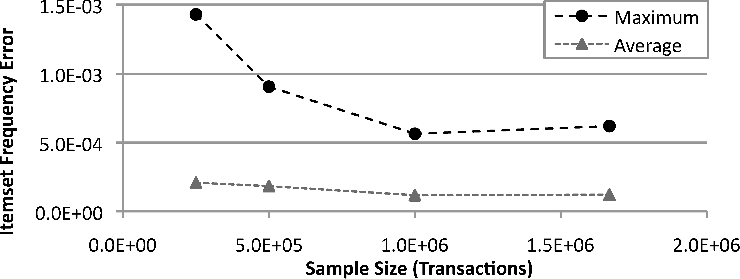
\includegraphics[width=0.75\linewidth]{vcmine/Fig2a}
    \caption{Absolute Itemset Frequency Error, BMS-POS dataset, $d=81$,
    $\theta=0.02$, $\varepsilon=0.01$, $\delta=0.1$.}
    {\label{fig:BMS-POS-absFI}}
  \end{subfigure}

 \begin{subfigure}[b]{\linewidth}
    \centering
    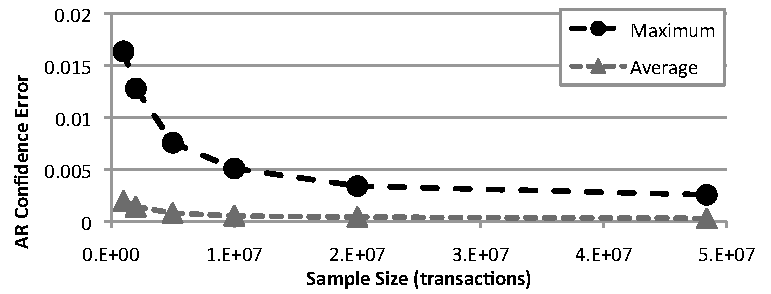
\includegraphics[width=0.75\linewidth]{vcmine/Fig2b}
    \caption{Relative Itemset Frequency Error, artificial dataset, $v=33$,
    $\theta=0.01$, $\varepsilon=0.05$, $\delta=0.1$.}
    \label{fig:artif-relFI}
  \end{subfigure}
  \caption{Absolute / Relative $\varepsilon$-close Approximation to
  $\FI(\Ds,\Itm,\theta)$} 
  \label{fig:fiapprox}
\end{figure}

Evaluating the strictness of the bounds to the sample size was the second goal
of our experiments. In Fig.~\ref{fig:BMS-POS-absFI} we show the behaviour of
the maximum frequency error as function of the sample size in the itemsets
obtained from samples using the method presented in Lemma~\ref{lem:absapproxfi}
(i.e., we are looking for an \emph{absolute} $\varepsilon$-close approximation
to $\FI(\Ds,\Itm,\theta)$). The rightmost plotted point corresponds to the
sample size computed by the theoretical analysis. We are showing the results
for the dataset BMS-POS replicated $40$ times (d-index $d=81$), mined with
$\theta=0.02$. It is clear from the picture that the guaranteed error bounds are
achieved even at sample sizes smaller than what computed by the analysis and
that the error at the sample size derived from the theory (rightmost plotted
point for each line) is one to two orders of magnitude smaller than the maximum tolerable
error $\varepsilon=0.01$. This can be exmplained by the fact that the d-bound
used to compute the sample size is in practice, as we argued in
Sect.~\ref{sec:vcminediscussion} a quite loose upper bound to the real VC-dimension.
%This fact seems to suggest that there is still room for
%improvement in the bounds to the sample size needed to achieve an absolute
%$\varepsilon$-close approximation to $\FI(\Ds,\Itm,\theta)$.
In Fig.~\ref{fig:artif-relFI}
we report similar results for the problem of computing a \emph{relative}
$\varepsilon$-close approximation to $\FI(\Ds,\Itm,\theta)$ for an artificial
dataset whose range space has VC-dimension $v$ equal to the length of the
longest transaction in the dataset, in this case $33$. The dataset contained 100
million transactions. The sample size, given by Lemma~\ref{lem:relapproxfi},
was computed using $\theta=0.01$, $\varepsilon=0.05$, and $\delta=0.1$.
The conclusions we can draw from the results for the behaviour of the
relative frequency error are similar to those we got for the absolute case.
For the case of absolute and relative $\varepsilon$-close approximation to
$\TOPK(\Ds,\Itm,K)$, we observed results very similar to those obtained for
$\FI(\Ds,\Itm,\theta)$, as it was expected, given the closed connection between
the two problems. 

\begin{figure}[htb]
  \centering
  \begin{subfigure}[b]{\linewidth}
    \centering
    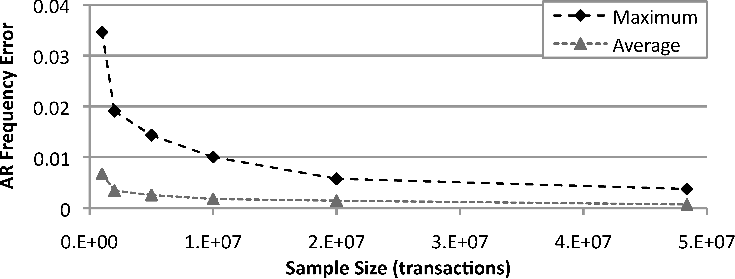
\includegraphics[width=0.75\linewidth]{vcmine/Fig3a}
    \caption{Relative Association Rule Frequency Error}
    \label{fig:artif-relAR-freq}
  \end{subfigure}

  \begin{subfigure}[b]{\linewidth}
    \centering
    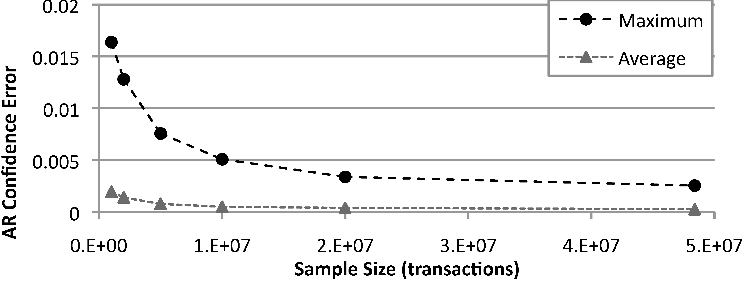
\includegraphics[width=0.75\textwidth]{vcmine/Fig3b}
    \caption{Relative Association Rule Confidence Error}
    \label{fig:artif-relAR-conf}  
  \end{subfigure}
  \caption{ Relative $\varepsilon$-close approximation to
  $\AR(\Ds,\Itm,\theta,\gamma)$, artificial dataset, $v=33$, $\theta=0.01$,
  $\gamma=0.5$, $\varepsilon=0.05$, $\delta=0.1$.} \label{fig:ar}
\end{figure}

The results of the experiments to evaluate our method to extract a relative
$\varepsilon$-close approximation to $\AR(\Ds,\Itm,\theta,\gamma)$ are presented
in Fig.~\ref{fig:artif-relAR-freq}~and~\ref{fig:artif-relAR-conf}. The same
observations as before hold for the relative
frequency error, while it is interesting to note that the relative confidence
error is even smaller than the frequency error, most possibly because the
confidence of an association rule is the ratio between the frequencies of two
itemsets that appear in the same transactions and their sample frequencies will
therefore have similar errors that cancel out when the ratio is computed.
Similar conclusions can be made for the absolute $\varepsilon$-close
approximation case.

From
Fig.~\ref{fig:BMS-POS-absFI},~\ref{fig:artif-relFI},~\ref{fig:artif-relAR-freq},~and~\ref{fig:artif-relAR-conf}
it is also possible to appreciate that, as the sample gets smaller, the maximum
and the average errors in the frequency and confidence estimations increase.
This suggests that using a fixed sampling rate or a fixed sample size can not
guarantee good results for any $\varepsilon$: not only the estimation of the
frequency and/or of the confidence would be quite off from the real value, but
because of this, many itemsets that are frequent in the original dataset may be
missing from the output collection and many spurious (very infrequent) itemsets
may be included in it.

The major motivating intuition for the use of sampling in market basket analysis
tasks is that mining a sample of the dataset is faster than mining the entire
dataset. Nevertheless, the mining time does not only depend on the number of
transactions, but also on the number of frequent itemsets. Given that our
methods suggest to mine the sample at a lowered minimum frequency threshold,
this may cause an increase in running time that would make our method not useful
in practice, because there may be many more frequent itemsets than at the
original frequency threshold. We performed a number of experiments to evaluate
whether this was the case and present the results in Fig.~\ref{fig:runtime}. 
We mined the artificial dataset introduced before for different values of $\theta$,
and created samples of size sufficient to obtain a relative $\varepsilon$-close
approximation to $\FI(\Ds,\Itm,\theta)$, for $\varepsilon=0.05$ and
$\delta=0.1$. Figure~\ref{fig:runtime} shows the time needed to mine the large
dataset and the time needed to create and mine the samples. It is possible to
appreciate that, even considering the sampling time, the speed up achieved by
our method is around the order of magnitude (i.e. 10x speed improvement),
proving the usefulness of sampling. Moreover, given that the sample size, and
therefore the time needed to mine the sample, does not grow with the size of the
dataset as long as the d-bound remains constant, that the d-index computation
can be performed online, and that the time to create the sample can be made
dependent only on the sample size using Vitter's Method D
algorithm~\citep{Vitter87}, our method is very scalable as the dataset grows, and
the speed up becomes even more relevant because the mining time for the large
dataset would instead grow with the size of the dataset.

\begin{figure}[tp]
  \centering
  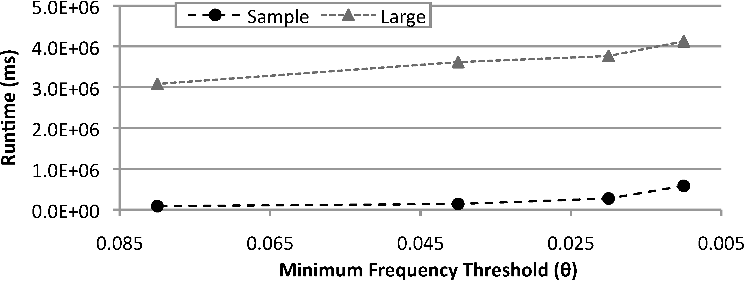
\includegraphics[width=0.75\textwidth]{vcmine/Fig4}
  \caption{Runtime Comparison. The sample line includes the sampling time.
  Relative approximation to FIs, artificial dataset, $v=33$, $\varepsilon=0.05$,
  $\delta=0.1$}
  \label{fig:runtime}
\end{figure}

Comparing our results to previous work we note that the bounds generated by our
technique are always linear in the VC-dimension $v$ associated with the dataset.
As reported in Table~\ref{table:comparsamsizeform}, the best previous
work~\citep{ChakaravarthyPS09} presented bounds that are linear in the maximum
transaction length $\Delta$ for two of the six problems studied here.
Figures~\ref{fig:compareSamSizeTheta} and~\ref{fig:compareSamSizeEpsilon} show
a comparison of the actual sample sizes for relative $\varepsilon$-close
approximations to $\FI(\Ds,\Itm,\theta)$ for as function of $\theta$ and
$\varepsilon$. To compute the points for these figures, we set $\Delta=v=50$,
corresponding to the worst possible case for our method, i.e., when the
VC-dimension of the range space associated to the dataset is exactly equal to
the maximum transaction length. We also fixed $\delta=0.05$ (the two methods
behave equally as $\delta$ changes). For Fig.~\ref{fig:compareSamSizeTheta}, we
fixed $\varepsilon=0.05$, while for Fig.~\ref{fig:compareSamSizeEpsilon} we
fixed $\theta=0.05$. From the Figures we can appreciate that both bounds have
similar, but not equal, dependencies on $\theta$ and $\varepsilon$. More
precisely the bound we present is less dependent on $\varepsilon$
and only slightly more dependent on $\theta$. It also evident that the sample
sizes given by the bound we present are always much smaller than
those presented in~\citep{ChakaravarthyPS09} (the vertical axis has logarithmic
scale). In this comparison we used $\Delta=v$, but almost all real datasets
we encountered have $v\ll\Delta$ as shown in Table~\ref{tab:deltadrealds} which
would result in a larger gap between the sample sizes provided by the two
methods. On the other hand, we should mention that the sample size given
by~\citep{ChakaravarthyPS09} can be slightly optimized by using a stricter
version of the Chernoff bound, but this does not change the fact that it
depends on the maximum transaction length rather than on the VC-Dimension.

\begin{figure}[htb]
  \centering
  \begin{subfigure}[b]{\linewidth}
    \centering
    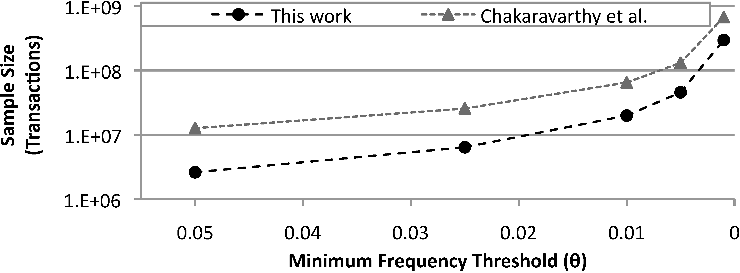
\includegraphics[width=0.75\linewidth]{vcmine/Fig5a}
    \caption{Sample size as function of $\theta$, $\varepsilon=0.05$}
     \label{fig:compareSamSizeTheta}
   \end{subfigure}

  \begin{subfigure}[b]{\linewidth}
    \centering
    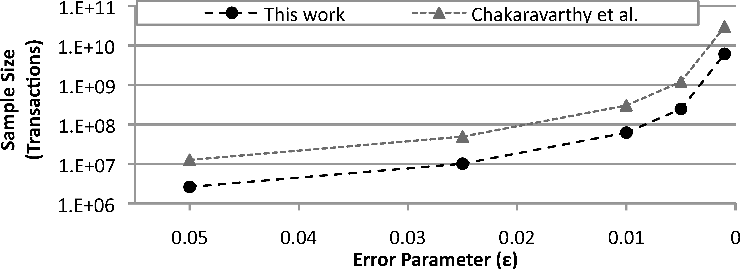
\includegraphics[width=0.75\linewidth]{vcmine/Fig5b}
    \caption{Sample size as function of $\varepsilon$, $\theta=0.05$}
    \label{fig:compareSamSizeEpsilon}
  \end{subfigure}
  \caption{Comparison of sample sizes for relative $\varepsilon$-close approximations to
  $\FI(\Ds,\Itm,\theta)$. $\Delta=v=50$, $\delta=0.05$.}
  \label{fig:compareSamSize}
\end{figure}

\begin{table}[hbt]
\centering
\caption{Values for maximum transaction length $\Delta$ and d-bound $q$ for real datasets}
\label{tab:deltadrealds}

\begin{tabular}{lcccccccc}
  \toprule
  & accidents & BMS-POS & BMS-Webview-1 & kosarak & pumsb* & retail & webdocs \\
  \midrule
  $\Delta$ & 51 & 164 & 267 & 2497 & 63 & 76 & 71472 \\
  $q$ & 46 & 81 & 57 & 443 & 59 & 58 & 2452 \\ 
  \bottomrule
\end{tabular}
\end{table}

\section{Conclusions}\label{sec:vcmineconcl}
In this chapter we presented a novel technique to derive random sample sizes
sufficient to easily extract high-quality approximations of the (top-$K$)
frequent itemsets and of the collection of association rules. The sample size
are linearly dependent on the VC-Dimension of the range space associated to the
dataset, which is upper bounded by the maximum integer $d$ such
that there at least $d$ transactions of length at least $d$ in the dataset. This 
bound is tight for a large family of datasets.  

We used theoretical tools from statistical learning theory to develop a very
practical solution to an important problem in computer science. The practicality
of our method is demonstrated in the extensive experimental evaluation which
confirming our theoretical analysis and suggests that in practice it is possible
to achieve even better results than what the theory guarantees. 
%Moreover, we
%used this method as the basic building block of an algorithm for the
%MapReduce~\citep{DeanS04} distributed/parallel framework of computation.
%PARMA~\citep{RiondatoDFU12}, our MapReduce algorithm, computes an absolute
%$\varepsilon$-approximation of the collection of FIs or ARs by mining a number
%of small random samples of the dataset in parallel and then aggregating and
%filtering the collections of patterns that are frequent in the samples. It
%allows to achieve very high-quality approximations of the collection of interest
%with very high confidence while exploiting and adapting to the available
%computational resources and achieving a high level of parallelism, highlighted 
%by the quasi-linear speedup we measured while testing PARMA.

Samples of size as computed by our methods can be used to mine approximations
of other collection of itemsets, provided that one correctly define the
approximation taking into account the guarantees on the estimation of the
frequency provided by the $\varepsilon$-approximation theorem. For example, one
can can use techniques like those presented in~\citep{MampaeyTV11} on a sample
to obtain a small collection of patterns that describe the dataset as best as
possible.

%We believe that methods and tools developed in the context of computational
%learning theory can be applied to many problems in data mining, and that results
%traditionally considered of only theoretical interest can be used to obtain very
%practical methods to solve important problems in knowledge discovery.

It may be possible to develop procedures that give a stricter upper bound to the
VC-dimension for a given dataset, or that other measures of sample complexity
like the triangular rank~\citep{NewmanR12}, shatter coefficients, or Rademacher
inequalities~\citep{BoucheronBL05}, can suggest smaller samples sizes. 

In the next chapter we build on the results presented here to develop and
analyze a fast and scalable algorithm for approximate FIs and ARs mining that
leverages on the power of the MapReduce distributed/parallel framework to
achieve very high accuracy and confidence while exploiting the available
computational resources.

In Ch.~\ref{ch:realfis} we flip the way we look at the itemsets mining problem
and present a method to avoid the inclusion of \emph{false positives} (itemsets
that are frequent only by chance) in the output.

%\paragraph{Acknowledgements.} The authors are thankful to Luc De Raedt for
%suggesting the connection between itemsets and monotone monomials. We also thank
%the anonymous reviewers for their many suggestions and comments for the
%improvement of this work.


\chapter{PARMA: a parallel randomized algorithm for approximate association
rules mining in MapReduce}\label{ch:parma}

\iffalse
\begin{abstract}
%The task of (top-K) Frequent Itemsets (FI's) and Association Rules (AR's) mining
%is a well-studied problem in computer science. The goal to discover a set of
%inference rules among sets of items that make up transactions in a dataset.
%There have been many algorithms proposed over the years to exactly solve this
%problem, both for sequential and parallel/distributed execution.
%The sequential algorithms suffer from a lack of scalability as the dataset size
%increase while the parallel methods often end up replicating large amounts of
%data in order to make the computation parallel. 
%We present a novel randomized parallel technique for mining Frequent Itemsets
%and Association Rules. Our algorithm, PARMA, achieves
%near-linear speedup while avoiding costly replication of data. PARMA does this
%by creating multiple small random samples of the transactional dataset and running
%a mining algorithm on the samples independently and in parallel. The resulting
%collections of Frequent Itemsets or Association Rules from each sample are aggregated and filtered to
%provide a single collection in output. Because PARMA mines random subsets of the
%dataset, the final result is an approximation of the exact solution. Our
%probabilistic analysis shows that PARMA provides tight guarantees on the quality
%of the approximation. The end user specifies accuracy and confidence parameters
%and PARMA computes an approximation of the collection of interest that satisfies
%these parameters. We formulated and implemented the algorithm in the MapReduce
%parallel computation framework. Our experimental results show that in practice the
%quality of the approximation is even higher than what can be analytically
%guaranteed. We demonstrate the correctness and scalability of PARMA by testing
%it on several synthetic datasets of varying size and complexity. We compare our results
%to two previously proposed exact parallel mining algorithms in MapReduce. 

Frequent Itemsets and Association Rules Mining (FIM) is a key task in knowledge
discovery from data. As the dataset grows, the cost of solving this task is
dominated by the component that depends on the number of transactions in the dataset.
%Part of the cost (\emph{scanning}) is due to the number of transaction in the
%dataset, and increases at least linearly with it. Another part (\emph{mining})
%is due to the number of Frequent Itemsets or Association Rules in the dataset.
%This is a caractheristic of the process that generated the data and of the
%user-speficied frequency and confidence thresholds. If the process and the
%thresholds do not change or change slowly, the number of FI's and AR's does not
%change as the number of transaction in the dataset grows, and so this part of
%the cost does not change. This implies that, as the dataset becomes larger and
%larger, the \emph{scanning} cost becomes dominant over the \emph{mining}
%cost.
%Many algorithms exist to solve the FIM task using different
%approaches, but they do not scale well on  the huge datasets available today as
%the dependency of their running times on the size of the dataset make them
%unsuitable for very large collections of transactions. 
We address this issue by proposing PARMA, a parallel algorithm for the MapReduce
framework, which scales well with the size of the dataset (as number of
transactions) while minimizing data replication and communication cost. PARMA
cuts down the dataset-size-dependent part of the cost by using a random sampling
approach to FIM. Each machine mines a small random sample of the dataset, of
size independent from the dataset size. The results from each machine are then
filtered and aggregated to produce a single output collection. The output will
be a very close approximation of the collection of Frequent Itemsets (FI's) or
Association Rules (AR's) with their
frequencies and confidence levels. The quality of the output is
probabilistically guaranteed by our analysis to be within the user-specified
accuracy and error probability parameters. The sizes of the random samples are
independent from the size of the dataset, as is the number of samples. They
depend on the user-chosen accuracy and error probability parameters and on the
parallel computational model. We implemented PARMA in Hadoop MapReduce and show
experimentally that it runs faster than previously introduced FIM algorithms for
the same platform, while 1) scaling almost linearly, and 2) offering even higher
accuracy and confidence than what is guaranteed by the analysis.
\end{abstract} 
\fi

We now extend the results presented in Chapter~\ref{ch:vcmine} and introduce
PARMA, a randomized parallel algorithm for approximate frequent itemset mining,
that makes the problem of Frequent Itemsets and Association Rules mining (FIM)
embarassingly parallel, thus exhibiting near-linear speedup with the number of
machines. PARMA combines random sampling and parallelization techniques in a
novel fashion.  It mines, in parallel, a set of small random samples and then
filters and aggregates the collections of frequent itemsets or association rules
obtained from each sample.  Our work is orthogonal to other approaches, like
PFP~\citep{LiWZZC08}, which focuses on parallelizing the mining phase in order
to decrease the corresponding component of the cost. Due to the use of random
sampling, the output of PARMA is an approximation of
the collection of FIs or ARs in the dataset, but leveraging on the results
presented in
Chapter~\ref{ch:vcmine}, PARMA offers tight probabilistic guarantees on the
quality of the approximated collections returned in output. In particular it
guarantees that the output is an $\varepsilon$-approximation of the real
collection with probability at least $1-\delta$, where $\varepsilon$ and
$\delta$ are parameters specified by the user (see Section~\ref{sec:parmadef} for
formal definitions). 
PARMA is designed on
MapReduce~\citep{DeanG08}, a novel parallel/distributed architecture that has
raised significant interest in the research and industry communities. MapReduce
is capable of handling very large datasets and efficiently executing parallel
algorithms like PARMA.

To our knowledge PARMA is the first algorithm to exploit the combination of
random sampling and parallelization for the task of Association Rules Mining. 

A number of previous works explored either parallel
algorithms~\citep{BuehrerPTKS07,CongHHP05,EHZaiane06,FangEtAl08,LiuLZT07,OzkuralUA11,JinYA05,Zaki99}
or random
sampling (see Sect.~\ref{sec:vcmineprevwork})
for the FIM task, but the two approaches have been seen somewhat orthogonal
until today. In PARMA, the disadvantages of either approach are evened out by
the advantages of the other. In the spirit of \emph{moving computation to the
data} to minimize communication, we avoid data replication, and preserve the
advantages of parallelization by using of multiple independent small random
samples of the dataset which are mined in parallel and have only their results
aggregated. Similarly, we are not subject to the inherent trade-off between the
size of the random sample and the accuracy of the approximation that can be
obtained from it, as PARMA would only have to mine more samples of the same size
in parallel to get higher quality approximations.

Although PARMA is not the first algorithm to use MapReduce to solve the
FIM task, it differs from and enhances previous
works~\citep{CryansRC10,GhotingKPK11,Hammoud11,LiWZZC08,LiZ11,YangLF10,ZhouZCLF10}
in two crucial aspects. First, it significantly reduces the data that is
replicated and transmitted in the \emph{shuffle} phase of MapReduce.  Second,
PARMA is not limited to the extraction of Frequent Itemsets but can also
directly compute the collection of Association Rules in MapReduce. In previous
works, association rules had to be created sequentially after the Frequent
Itemsets had been computed in MapReduce. 

We conducted an extensive experimental evaluation to test the relative
performance, scalability and accuracy of PARMA across a wide range of
parameters and datasets. Our results suggest that PARMA can
significantly outperform exact mining solutions, has
near-linear speedup, and, as data and nodes are scaled together, is
able to achieve near constant runtimes. Also, our accuracy evaluation
shows that PARMA consistently computes approximated collections
of higher quality than what can be analytically guaranteed.

In this chapter:
\begin{enumerate}
\item We present PARMA, the first randomized MapReduce algorithm for discovering
  approximate collections of frequent itemsets or association rules with
  near-linear speedup.
\item We provide analytical guarantees for the quality of the approximate
  results generated by the algorithm.
\item We demonstrate the effectiveness of PARMA on many datasets and compare
  the performance of our implementation to that of several exact FIM algorithms
  on MapReduce.
\end{enumerate}


\section{Previous Work}
\label{sec:parmarelated}
We already discussed the relevant previous work about general FI mining and the
use of sampling for this task in Sect.~\ref{sec:vcmineprevwork}. We now focus on the
contributions that are relevant for this chapter: the mining of FIs in a
parallel or distributed setting, the MapReduce framework of computation, and its
use to compute FIs and ARs.

The use of parallel and/or distributed algorithms for Association Rules Mining comes from the
impossibility to handle very large datasets on a single machine. Early
contributions in this area are presented in a survey by~\citet{Zaki99}.
In recent years, the focus shifted to exploit architecture advantages as much as
possible, such as shared memory~\citep{JinYA05}, cluster
architecture~\citep{BuehrerPTKS07} or the massive parallelism of
GPUs~\citep{FangEtAl08}. The main goal is to avoid communication
between nodes as much as possible and minimize the amount of data that are moved
across the 
network~\citep{CongHHP05,EHZaiane06,LiuLZT07,OzkuralUA11}.

The MapReduce~\citep{DeanG08} paradigm enjoys widespread success
across both industry and academia. Research communities in many different
fields uses this novel approach to distributed/parallel computation to develop
algorithms to solve important problems in computer
science~\citep{ChierichettiKT10,ChuKLYBNO06,GoodrichSZ11,LinS10,PietracaprinaPRSU12}.
Not only MapReduce can easily perform computation on very large datasets, but it
is also extremely suited in executing embarassingly parallel algorithms which
make a very limited use of communication. PARMA fits in this description so
MapReduce is an appropriate choice for it.

A number of previous
works~\citep{CryansRC10,GhotingKPK11,Hammoud11,LiWZZC08,LiZ11,YangLF10,ZhouZCLF10}
looked at adapting APriori and FP-growth to the MapReduce setting. Somewhat
naively, some authors~\citep{CryansRC10,LiZ11,YangLF10} suggest a distributed/parallel
counting approach, i.e. to compute the support of every itemset in the dataset
in a single MapReduce round. This algorithm necessarily incurs in a huge data
replication, given that an exponential number of messages are sent to the
reducers, as each transaction contains a number of itemsets that is exponential
in its length. A different adaptation of APriori to MapReduce is presented
in~\cite[Chap.4]{Hammoud11}: similarly to the original formulation of APriori,
at each round $i$, the support for itemsets of length $i$ is computed, and those
that are deemed frequent are then used to generate candidate frequent itemsets
of length $i+1$, although outside of the MapReduce environment. Apart from this,
the major downsides of such approach are that some data replication still
occurs, slowing down the shuffling phase, and that the algorithm does not
complete until the longest frequent itemset is found. Given that length is not
known in advance, the running time of the algorithm can not be
computed in advance. Also the entire dataset needs to be scanned at each round, which
can be very expensive, even if it is possible to keep additional data structures
to speed up this phase.  

An adaptation of FP-Growth to MapRreduce called PFP is presented by~\citet{LiWZZC08}. First,
a parallel/distributed counting approach is used to compute the frequent items,
which are then randomly partitioned into groups. Then, in a single MapReduce
round the transactions in the dataset are used to generate group-dependent
transactions. Each group is assigned to a reducer and the corresponding
group-dependent transactions are sent to this reducer which then builds the
local FP-tree and the conditional FP-trees recursively, computing the frequent
patterns. The group-dependent transactions are such that the local FP-trees and
the conditional FP-trees built by different reducers are independent. This
algorithm suffers from a data replication problem: the number of
group-dependent transactions generated for each single transaction is
potentially equal to the number of groups. This means that the dataset may be
replicated up to a number of times equal to the number of groups, resulting in a
huge amount of data to be sent to the reducers and therefore in a slower
synchronization/communication (\emph{shuffle}) phase, which is usually the most
expensive in a MapReduce algorithm.  Another practical downside of PFP is that
the time needed to mine the dependent FP-tree is not uniform across the groups.
An empirical solution to this load balancing problem is presented
by~\citet{ZhouZCLF10}, although with no guarantees and by computing the groups
outside the MapReduce environment. An implementation of the PFP algorithm as
presented in~\citep{LiWZZC08} is included in Apache Mahout
(\url{http://mahout.apache.org}). \citet{GhotingKPK11} present
an high-level library to perform various machine learning and data mining tasks
using MapReduce. They show how to implement the Frequent Itemset Mining task
using their library. The approach is very similar to that in~\citep{LiWZZC08},
and the same observations apply about the performances and downsides of this
approach.


\section{Preliminaries} \label{sec:parmadef}
In this chapter we show how to extract $\varepsilon$-close approximations of the
collection of (top-$k$) Frequent Itemsets and Association Rules using MapReduce. See
Sect.~\ref{sec:vcminepreldm} for definitions about FIs, ARs. We slightly
generalize the definitns of $\varepsilon$-close
approximation of $\FI(\Ds,\Itm,\theta)$ (Def.~\ref{def:vcmineapproxfi}) and of
$\AR(\Ds,\Itm,\theta,\gamma)$ (Def.~\ref{def:vcmineapproxfi}) as follows.

\begin{definition}\label{def:parmaeapproxfi}
  Given two parameters $\varepsilon_1,\varepsilon_2\in(0,1)$, an \emph{absolute}
  (resp.~\emph{relative}) \emph{
  $(\varepsilon_1,\varepsilon_2)$-close approximation} of
  $\FI(\Ds,\Itm,\theta)$ is a set $\mathcal{C}=\{(A, f_A, \mathcal{K}_A) ~:~ A\in 2^\Itm,
  f_A\in\mathcal{K}_A\subseteq[0,1]\}$ of triplets $(A, f_A, \mathcal{K}_A)$ where
  $f_A$ approximates $f_\Ds(A)$ and $\mathcal{K}_A$ is an interval containing
  $f_A$ and $f_\Ds(A)$.
  $\mathcal{C}$ is such that:
  \begin{enumerate}
    \item $\mathcal{C}$ contains all itemsets appearing in
      $\FI(\Ds,\Itm,\theta)$;
    \item $\mathcal{C}$ contains no itemset $A$ with frequency $f_\Ds(A)<\theta -
      \varepsilon_1$ (resp.~ $f_\Ds(A)\le\theta(1-\varepsilon_1$);
    \item For every triplet $(A, f_A,\mathcal{K}_A)\in\mathcal{C}$, it holds
      \begin{enumerate}
       \item $|f_\Ds(A)-f_A|\le\varepsilon_2$ (resp.~
	 $|f_\Ds(A)-f_A|\le\varepsilon_2f_\Ds(A)$).
       \item $f_A$ and $f_\Ds(A)$ belong to $\mathcal{K}_A$.
       \item $|\mathcal{K}_A|\le 2\varepsilon_2$ (resp.~$|\mathcal{K}_A|\le
	 2\varepsilon_2f_\Ds(A)$).
     \end{enumerate}
  \end{enumerate}
  If $\varepsilon_1=\varepsilon_2=\varepsilon$ we refer to $\mathcal{C}$ 
  as an absolute (resp.~relative) $\varepsilon$-close approximation of
  $\FI(\Ds,\Itm,\theta)$.
\end{definition} 

Through~\eqref{eq:topkfiequiv} we have that an absolute (resp.~relative)
$(\varepsilon_1,\varepsilon_2)$-close approximation to
$\FI\left(\Ds,\Itm,f^{(K)}_\Ds\right)$ is an
$(\varepsilon_1,\varepsilon_2)$-approximation to $\TOPK(\Ds,\Itm,K)$.

For association rules, we generalize Def.~\ref{def:vcmineapproxar} as follows.
\begin{definition}\label{def:parmaeapproxar}
  Given two parameters $\varepsilon_1,\varepsilon_2\in(0,1)$ an
  \emph{absolute} (resp.~\emph{relative})
  \emph{$(\varepsilon_1,\varepsilon_2)$-close approximation} of $\AR(\Ds,\Itm,\theta,\gamma)$
  is a set \[\mathcal{C}=\{(W, f_W, \mathcal{K}_W, c_W, \mathcal{J}_W)~|~ 
  \mbox{AR } W, f_W\in\mathcal{K}_W, c_W\in\mathcal{J}_W\}\]
  of tuples $(W, f_W, \mathcal{K}_W, c_W, \mathcal{J}_W)$ where $f_W$ and $c_W$
  approximate $f_\Ds(W)$ and $c_\Ds(W)$ respectively and belong to
  $\mathcal{K}_W\subseteq[0,1]$ and
  $\mathcal{J}_W\subseteq[0,1]$ respectively. $\mathcal{C}$ is such
  that:
  \begin{enumerate}
    \item $\mathcal{C}$ contains all association rules appearing in
      $\AR(\Ds,\Itm,\theta,\gamma)$;
    \item $\mathcal{C}$ contains no association rule $W$ with frequency
      $f_\Ds(W)<\theta-\varepsilon_1$ (resp.~$f_\Ds(W)<\theta(1-\varepsilon_1)$);
    \item For every tuple $(W, f_W,\mathcal{K}_W,
      c_W,\mathcal{J}_W)\in\mathcal{C}$, it holds
      $|f_\Ds(W)-f_W|\le\varepsilon_2$ and $|\mathcal{K}_W|\le 2\varepsilon_2$
      (resp.~$|f_\Ds(W)-f_W|\le\varepsilon_2f_Ds(W)$ and $|\mathcal{K}_W|\le
      2\varepsilon_2f_\Ds(W)$).
    \item $\mathcal{C}$ contains no association rule $W$ with confidence 
      $c_\Ds(W)<\gamma-\varepsilon_1$ (resp.~$c_\Ds(W)<\gamma(1-\varepsilon_1)$);
    \item For every tuple $(W, f_W,\mathcal{K}_W,
      c_W,\mathcal{J}_W)\in\mathcal{C}$, it holds
      $|c_\Ds(W)-c_W|\le\varepsilon_2$ and $|\mathcal{J}_W|\le 2\varepsilon_2$
      (resp.~$|c_\Ds(W)-c_W|\le\varepsilon_2c_Ds(W)$ and $|\mathcal{J}_W|\le
      2\varepsilon_2c_\Ds(W)$).
  \end{enumerate}
    If $\varepsilon_1=\varepsilon_2=\varepsilon$ we refer to $\mathcal{C}$ 
  as an absolute (resp.~relative) $\varepsilon$-close approximation of
  $\AR(\Ds,\Itm,\theta,\gamma)$.
\end{definition}

It is easy to see that it is possible to modify Lemmas~\ref{lem:absapproxfi}, \ref{lem:relapproxfi},
\ref{lem:absapproxtopk}, \ref{lem:relapproxtopk}, \ref{lem:absapproxar}, and
\ref{lem:relapproxar} to return absolute or relative
$(\varepsilon,\varepsilon/2)$-close approximations of the relevant collections
of FIs or ARs.

\subsection{MapReduce}
MapReduce is a programming paradigm and an associated parallel
and distributed implementation for developing and executing parallel algorithms
to process massive datasets on clusters of commodity machines~\citep{DeanG08}.
Algorithms are specified in MapReduce using two functions, $\mathbf{map}$ and
$\mathbf{reduce}$. The input is seen as a sequence of ordered key-value pairs
$(k,v)$. The $\mathbf{map}$ function takes as input one such $(key,value)$ pair
at a time, and can produce a finite multiset of pairs
$\{(k_1,v_1),(k_2,v_2),\cdots\}$. Let $\mathcal{U}$ be the multiset
union of all the multisets produced by the $\mathbf{map}$ function when applied
to all input pairs. We can partition $\mathcal{U}$ into sets
$\mathcal{U}_{\bar{k}}$ indexed by a particular key $\bar{k}$.
$\mathcal{U}_{\bar{k}}$ contains all and only the values $v$ for which there are pairs
$(\bar{k},v)$ with key $\bar{k}$ produced by the function $\mathbf{map}$
($\mathcal{U}_{\bar{k}}$ is a multiset, so a particular value $v$ can appear
multiple times in $\mathcal{U}_{\bar{k}}$). The $\mathbf{reduce}$ function takes as
input a key $\bar{k}$ and the multiset $\mathcal{U}_{\bar{k}}$ and produce another set
$\{(k_1,v_1),(k_2,v_2),\cdots\}$. 
The output of $\mathbf{reduce}$ can be used as
input for another (different) $\mathbf{map}$ function to develop MapReduce
algorithms that complete in multiple \emph{rounds}. 
By definition, the $\mathbf{map}$ function can be executed in parallel for each
input pair. In the same way, the computation of the output of $\mathbf{reduce}$
for a specific key $k^*$ is independent from the computation for any other key $k'\neq
k^*$, so multiple copies of the $\mathbf{reduce}$ function can be executed
in parallel, one for each key $k$. We denote the machines executing the
$\mathbf{map}$ function as \emph{mappers} and those executing the
$\mathbf{reduce}$ function as $\emph{reducers}$. The latter will be indexed by
the key $k$ assigned to them, i.e., reducer $r$ processes the multiset
$\mathcal{U}_r$. The data produced by the mappers are split by key and
sent to the reducers in the so-called \emph{shuffle} step. Some implementations, 
including Hadoop and the one described by Google~\citep{DeanG08}, use sorting in
the shuffle step to perform the grouping of map outputs by key.
The shuffle is transparent
to the algorithm designer but, since it involves the transmission of (possibly very
large amount of) data across the network, can be very expensive.


\section{Algorithm}
\label{sec:parmaparmaalgo}
In this section we describe and analyze PARMA, our algorithm for extracting
$\varepsilon$-approximations of $\FI(\Ds,\Itm,\theta)$,
$\TOPK(\Ds,\Itm,\theta)$, and $\AR(\Ds,\Itm,\theta,\gamma)$ from samples of a dataset
$\Ds$ with probability at least $1-\delta$. In this section we present the
variant for $\FI(\Ds,\Itm,\theta)$. The variants for the cases of $\TOPK(\Ds,\Itm,\theta)$ and
$\AR(\Ds,\Itm,\theta,\gamma)$ can be easily derived from the one
we present here. We outline them in Section~\ref{sec:parmaeapproxtopk}. Detailed
presentations for them will appear in the full version of the paper.

%\subsection{Motivation} 
%As we said in the introduction, we start from the observation that the cost of
%frequent itemsets mining can be split in two independent components: the
%\emph{scanning} cost and the \emph{mining cost}. We can see the cost of a step
%of a mining algorithm as being accounted to either of the scanning or the mining
%component depending on the nature of the step. If the step involves looking, touching, or
%in any way operating on a transaction in the dataset, then it gets
%accounted to the scanning component of the cost. Examples of this type of
%operation include the scanning of the dataset to build the FP-Tree in
%FP-Growth~\cite{HanPY00} or to compute the actual frequencies of candidate frequent
%itemsets in APriori~\cite{AgarwalIS93}. On the other hand, when the algorithm is
%working on computing (candidate) frequent itemsets or their frequencies, then
%the cost is accounted to the mining component. No access to the dataset is
%needed in these steps. This kind of steps include all the operation performed on
%the FP-Tree once it has been generated, and the creation of candidate itemsets
%of length $i+1$ at the end of phase $i$ in APriori. While in APriori operations
%of either type are heavily interleaved, in FP-Growth there is a clear separation
%between the two: the cost of constructing the FP-Tree is accounted to the scanning component,
%while any successive operation is part of the mining component. It is easy to
%see this distinction, as dataset is no longer needed once the FP-Tree has been
%built. Because of this clear separation, in this discussion we will refer to
%FP-Growth, but a similar reasoning can be done for APriori. It is clear that the
%scanning component of the cost is heavily dependent on the number of
%transactions in the dataset, and independent on the other variables of the
%instance of the problems, like the number of items, the number and distribution
%of frequent itemsets, the frequency threshold, and the underlying process that
%generated the transactions. On the other hand, the mining component is
%independent on the dataset size, and instead depends on all the above
%parameters. In particular, notice that if we keep them constant, and just
%increase the dataset size, the mining component will not change. This is clear
%in FP-Growth, as the number of operations performed on the FP-Tree depends on
%the number and distribution of the frequencies of the itemsets, which were
%fixed, but not on the size of the dataset. Because of this, as the dataset
%grows, the scanning component of the cost becomes more and more relevant and
%dominates the mining component. In many practical settings for FIM, the process
%generating the data, and therefore the number and frequency distribution of the
%frequent itemsets grows much slower than the size of the dataset. For example,
%the number of items sold by an e-commerce website grows much slower than the
%number of purchases by customers, each of which corresponds to a transaction.
%Therefore the scanning component grows faster than the mining one, easily
%becoming the dominant. In conclusion, it is of the foremost importance to cut
%down the scanning cost in order to achieve better performances in FIM. This is
%exactly the main design goal of PARMA. PFP~\cite{LiWZZC08} focused instead of
%parallelizing the mining phase in order to decrease the corresponding component
%of the cost.

\subsection{Design}\label{subsec:parmadesign}
We now present the algorithmic design framework on which we developed PARMA and some design
decisions we made for speeding up the computation. 

\paragraph*{Model}When developing solutions for any computational problem,
the algorithm designer must always be aware of the trade-off between the available
computational resources and the performance (broadly defined) of the algorithm.
In the parallel computation setting, the resources are usually modeled through
the parameters $p$ and $m$, representing respectively the number of available
processors that can run in parallel and the amount of local memory available to
a single processor. In our case we will express $m$ in terms of the number of
transactions that can be stored in the main memory of a single machine.
When dealing with algorithms that use random samples of the input, the
performances of the algorithm are usually measured through the parameters
$\varepsilon$ and $\delta$. The former represents the desired accuracy of the
results, i.e., the maximum tolerable error (defined according to some distance
measure) in the solution computed by the algorithm using the random sample
when compared to an exact solution of the computational problem. The parameter
$\delta$ represents the maximum acceptable probability that the previously
defined error in the solution computed by the algorithm is greater than
$\varepsilon$. The measure we will use to evaluate the performances of PARMA in
our analysis is based on the concept of $\varepsilon$-approximation introduced in
Definition~\ref{def:parmaeapproxfi}.

\paragraph*{Trade-offs} We are presented with a trade-off between the parameters
$\varepsilon$, $\delta$, $p$, and $m$. To obtain a $\varepsilon$-approximation
with probability at least $1-\delta$, one must have a certain amount of computational resources,
expressed by $p$ and $m$. On the other hand, given $p$ and $m$, it is possible
to obtain $\varepsilon$-approximations with probability at least
$1-\delta$ only for values of $\varepsilon$ and $\delta$ larger than some
limits. By fixing any three of the parameters, it is possible to find the
best value for the fourth by solving an optimization problem. From
Lemma~\ref{lem:keythmfi} we know that there is a trade-off between
$\varepsilon$, $\delta$, and the size $w$ of a random sample from which it is
possible to extract a $(\varepsilon,\varepsilon/2)$-approximation to
$\FI(\Ds,\Itm,\theta)$ with probability at least $1-\delta$. If $w\le m$, then
we can store the sample in a single machine and compute the
$\varepsilon$-approximation there using Lemma~\ref{lem:keythmfi}. For some
combinations of values for $\varepsilon$ and $\delta$, though, we may have that
$w>m$, i.e. the sample would be too large to fit into the main memory of a single
processor, defeating one of the goals of using random sampling, that is to store
the set of transactions to be mined in main memory in order to avoid expensive disk
accesses. To address the issue of a single sample not fitting in memory, PARMA
works on multiple samples, say $N$ with $N\le p$, each of size $w\le m$ so that
{\bf 1)} each sample fits in the main memory of a single processor and {\bf 2)}
for each sample, it is possible to extract an
$(\varepsilon,\varepsilon/2)$-approximation of $\FI(\Ds,\Itm,\theta)$ from it
with probability at least $1-\phi$, for some $\phi>\delta$. In the first stage,
the samples are created and mined in parallel and the so-obtained collections of
Frequent Itemset are then aggregated in a second stage to compute the final output. This
approach is a perfect match for the MapReduce framework, given the limited
number of synchronization and
communication steps that are needed. Each
stage is performed in a single MapReduce round. The computational and data
workflow of PARMA is presented in Figure~\ref{fig:parmaoverview}, which we
describe in detail in the following paragraphs.

\begin{figure}[htb]
\centering
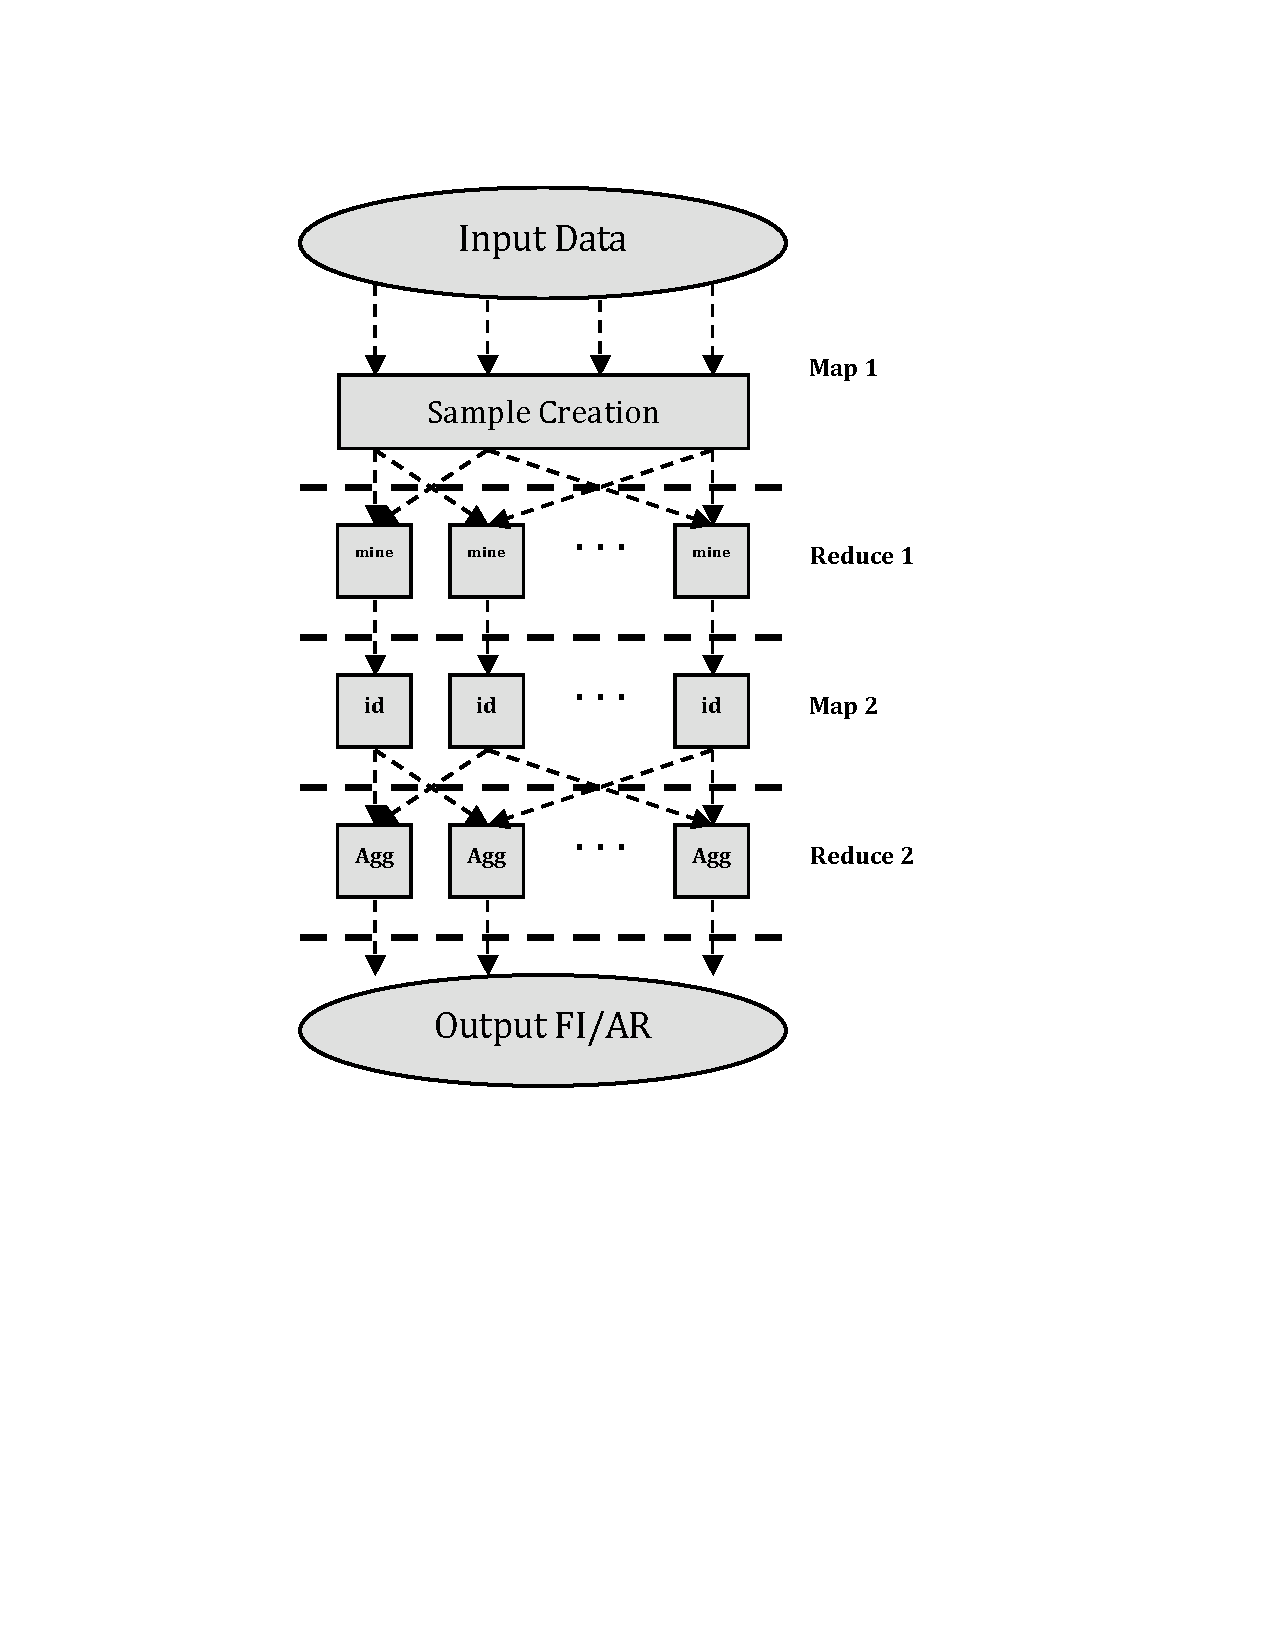
\includegraphics[width=0.3\textwidth]{parma/overview.pdf}
\caption{A system overview of PARMA. Ellipses represent data, squares represent
computations on that data and arrows show the movement of data through the
system.}
\label{fig:parmaoverview}
\end{figure}

  \begin{comment}
  The diagram is broken into 4 main computations which correspond to the
  Map and Reduce phases of the two MapReduce rounds in the algorithm. In
  the Map of Stage 1, a sample is created. In the Reduce of Stage 1, a
  mining algorithm is run on the subset of the sample created in the Map
  phase. This mining algorithm can be either frequent itemset mining or
  association rule mining, and as such is generically labeled mine. In
  the Map phase of Stage 2, the local frequent itemsets are sent to an
  identity mapper, and finally Aggregated in the Stage 2 Reduce to get a
  global set of frequent itemsets or assocation rules, depending on the
  mining algorithm used.
\end{comment}


\paragraph*{Computing $N$ and $w$} From the above discussion it should be clear
that, once $p$, $m$, $\varepsilon$ and $\delta$ have been fixed, there is a
trade-off between $w$ and $N$. In the MapReduce setting, often the most expensive
operation is the movement of data between the mappers and the reducers in the
shuffle phase. In PARMA, the amount of data to be shuffled corresponds to the
sum of the sizes of the samples, i.e., $Nw$, and to the amount of
communication needed in the aggregation stage. This second quantity is dependent
on the number of frequent itemsets in the dataset, and therefore PARMA has no
control over it. PARMA tries to minimize the first quantity when computing $N$ and
$w$ in order to achieve the maximum speed. It is still possible to minimize for
other quantities (e.g. $\varepsilon$ or $\delta$ if they have not been fixed),
but we believe the most effective and natural in the MapReduce setting is the
minimization of the communication.  This intuition was verified in our
experimental evaluation, where communication proved to be the dominant cost. We
can formulate the problem of minimizing $Nw$ as the following Mixed Integer Non
Linear Programming (MINLP) problem:
\begin{itemize}
  \item {\bf Variables:} non-negative integer $N$, real $\phi\in(0,1)$,
  \item {\bf Objective:} minimize $2N/\varepsilon^2 (d+\log(1/\phi))$.
  \item {\bf Constraints:}
    \begin{align}
      &N \le p \label{eq:parmaconstr1}\\
      &\phi \ge e^{-m\varepsilon^2/2 + d} \label{eq:parmaconstr2}\\
      &N(1-\phi)-\sqrt{N(1-\phi)2\log(1/\delta)} \ge N/2 + 1 \label{eq:parmaconstr3}
    \end{align}
\end{itemize}
Note that, because of our requirement {\bf 2)} on $w$, the sample size $w$ is directly
determined by $\phi$ through Lemma~\ref{lem:keythmfi}, so the trade-off is
really between $N$ and $\phi$, while $w$ does not appear in the above problem.
Since $\phi$ is a probability we restrict its
domain to the interval $(0,1)$, but it must also be such that the single sample size
$w$ is at most $m$, as required by {\bf 1)} and expressed by
Constraint~\eqref{eq:parmaconstr2}. The limit to the number of samples $N$ is expressed by
Constraint~\eqref{eq:parmaconstr1}. The last constraint~\eqref{eq:parmaconstr3} is a bit
more technical and the need for it will be evident in the analysis of the
algorithm. Intuitively, it expresses the fact that an itemset must appear in a
sufficiently high fraction (at least 1/2, possibly more) of the collections obtained from the samples in the
first stage in order to be included in the output collection. Due to the integrality constraint on
$N$, this optimization problem is not convex, although when the constraint it is
dropped the feasibility region is convex, and the objective function is convex.
It is then relatively easy and fast to find an integer optimal solution to the
problem using a global MINLP solver like BARON~\cite{baron}. 

%\paragraph{Overview} PARMA builds on a previous work~\cite{RiondatoU12} which
%presented algorithms to probabilistically extract $\varepsilon$-approximations
%of FI's and AR's using a random sample of the dataset, in a sequential setting.
%The size of the sample suggested in~\cite{RiondatoU12} work depends on the
%desidered accuracy and probability of error parameters $\varepsilon$ and
%$\delta$. When extremely accurate approximations are desired with a very low
%probability of error ($\varepsilon$ and $\delta$ are very small), the resulting
%sample may become too large to be easily handled by a single machine. By
%exploiting the parallel/distributed architecture of MapReduce, PARMA allows to
%obtain very high-confidence and extremely accurate approximations by first
%creating and mining a number of smaller samples in parallel using appropriately
%lowered frequency and confidence thresholds. For each sample, the collection
%obtained by mining it is a $(\varepsilon,\varepsilon/2)$-approximation of the
%desired collection of FI's or AR's with probability at least $1-\phi$, where
%$\phi\ge\delta$. In its second phase, PARMA aggregates these collections to
%obtain a single collection to be output. Although it can only offer the same
%analytical guarantees, in practice PARMA can return approximations of higher
%quality than what the sequential approach in~\cite{RiondatoU12} could do, thanks
%to the aggregation of multiple estimations of the frequencies and the
%confidences of the FI's and AR's. The aggregation allows for a decrease in the
%false positives discovery rate in the output collection and in improved accuracy
%in the estimation of the frequencies and of the confidences of FI's and AR's.
%Figure~\ref{fig:parmaoverview} shows a system overview of PARMA. The algorithm is
%described in details in the next few paragraphs.

%\begin{figure}[t]
%\centering
%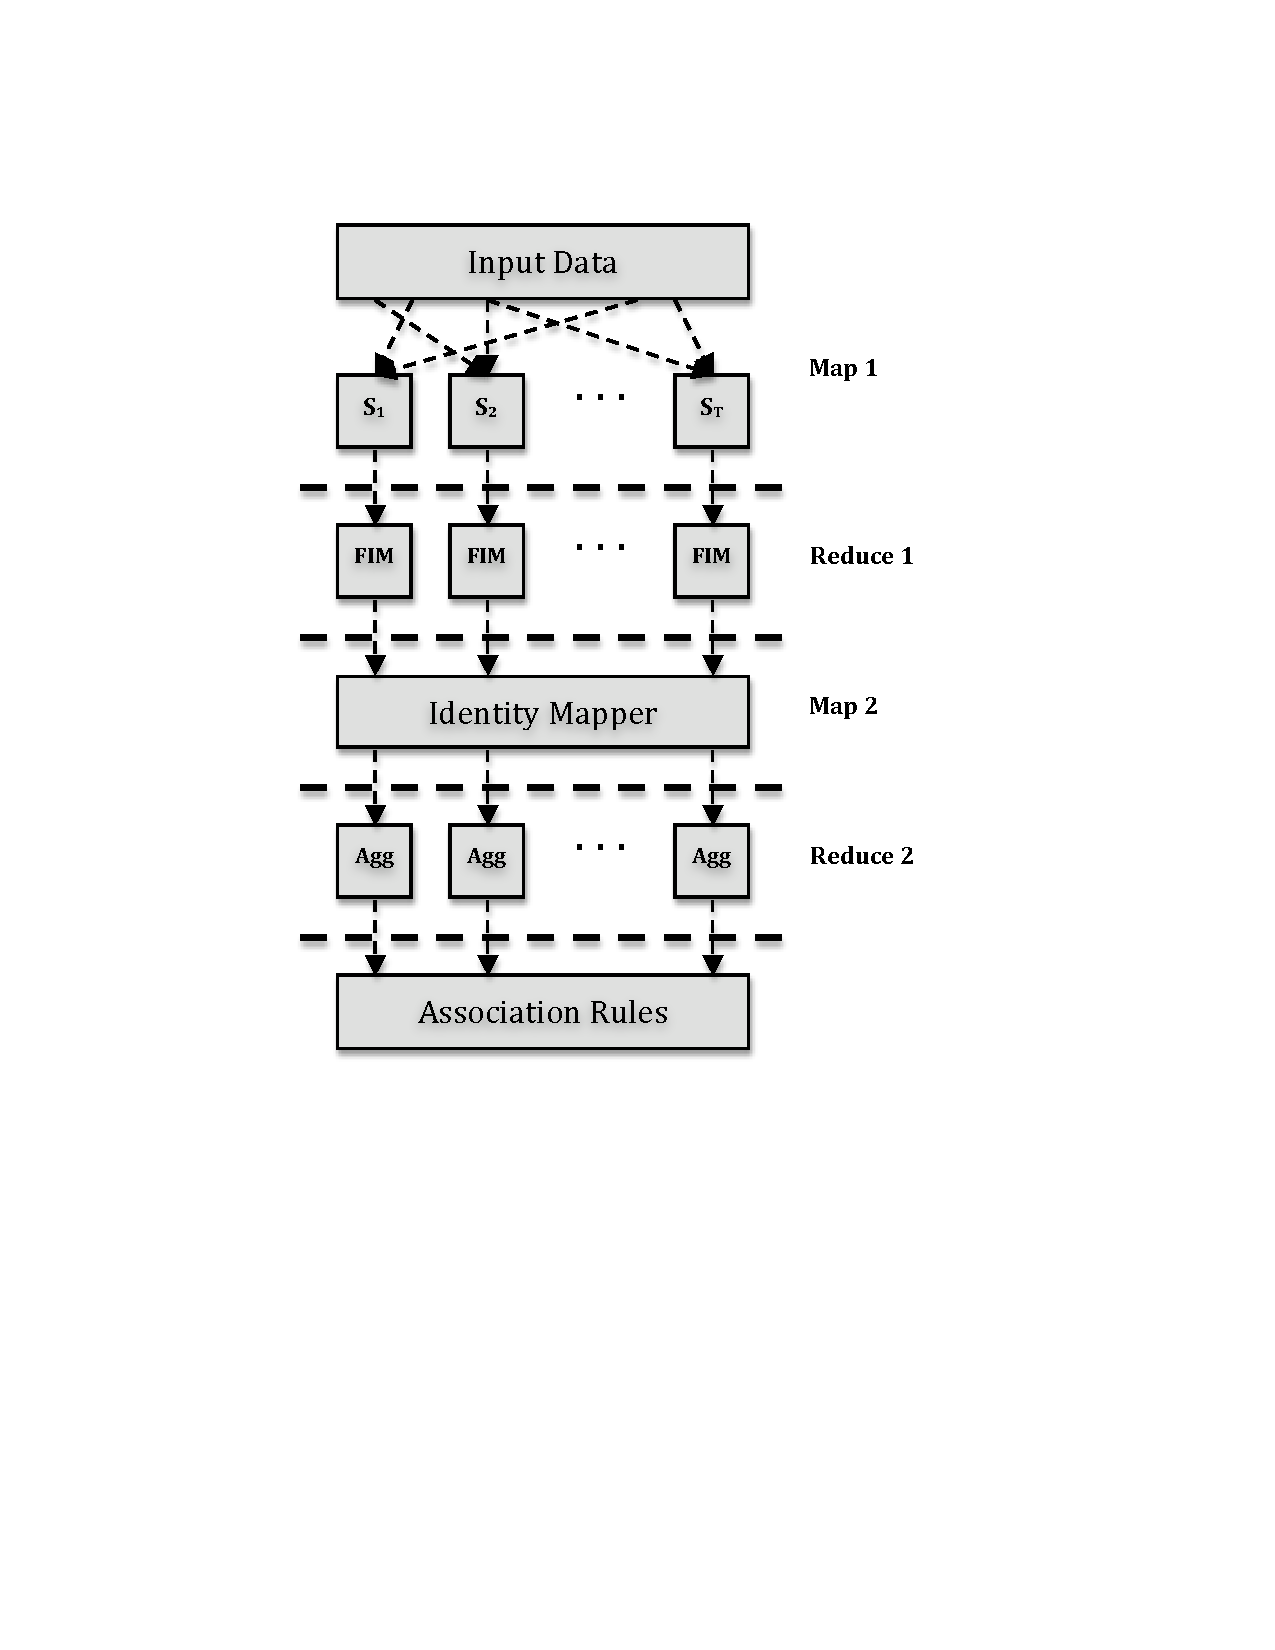
\includegraphics[width=0.45\textwidth]{parmm_overview}
%\caption{A system overview of PARMM.}
%\label{fig:parmaoverview}
%\end{figure}

%\paragraph{Parameters} PARMA has a number of input parameters, in addition
%to the expected parameters describing the ARM task, like the dataset $\Ds$, the
%minimum frequency threshold $\theta$ (or $K$ for Top-$K$ FI's mining) and the
%minimum confidence threshold $\gamma$ (only for mining AR's). The accuracy and
%the probability of error in the output of the algorithm are expressed by the two
%parameters $\varepsilon$ and $\delta$. The algorithm will return an
%$\varepsilon$-approximation of the desired collection of FI's or AR's with
%probability at least $1-\delta$. There are two additional parameters $m$ and $M$
%which control the behaviour of PARMA. They are respectively the maximum sample
%size (in number of transactions) that can be handled by a single machine in the
%MapReduce cluster and the maximum total sample size (i.e. the sum of the single
%sample sizes). The parameters $m$ and $M$ try to capture the computational power
%(more specifically the memory limitations) of the MapReduce cluster running
%PARMA. PARMA will use samples of size $w\le m$ and a number of samples $N$ such
%that $wN \le M$. One last parameter needed by PARMA is $d$,the maximum integer
%such that $\Ds$ has at least $d$ transactions of length at least $d$.

%We denote with $\phi$ the probability that the collection obtained from a
%of the samples is not an $\varepsilon$-approximation to the desired collection.
%For the case of $\FI(\Ds,\Itm,\theta)$, we can express $w$ as function of
%$\phi$, $\varepsilon$, and $d$~\cite{RiondatoU12}: 
%\begin{equation}\label{eq:parmasinglesamplesize}
%w=\frac{2}{\varepsilon^2}\left(d+\log\frac{1}{\phi}\right)
%\end{equation}
%Note how this expression is independent of $\theta$. Similar expressions of $w$
%can be obtained for the case of $\TOPK(\Ds,\Itm,K)$ and
%$\AR(\Ds,\Itm,\theta,\gamma)$~\cite{RiondatoU12}. The values for $\phi$, $w$,
%and $N$ are computed by minimizing the total number of sampled transactions
%$wN$, under some constraints (see below). Note that we will assume that 
%\[ m < \frac{2}{\varepsilon^2}\left(d + \log\frac{1}{\delta}\right)\]
%otherwise we would be able to obtain an $\varepsilon$-approximation with
%probability $1-\delta$ by mining just one sample using Lemma~\ref{lem:keythmfi}.

%\paragraph{Computing $w$ and $N$} One of the goals of PARMA is to minimize the
%amount of data that are sent from mappers to reducers. This is equivalent to minimize
%the total number of sampled transactions $wN$, where $w$ is the size of a single
%sample and $N$ is the number of samples we create. We can formulate the problem
%of minimizing $w$ as the following Mixed Integer Non Linear Programming (MINLP) 
%problem:
%\begin{itemize*}
%  \item {\bf Variables:} non-negative integer $N$, real $\phi\in(0,1)$,
%  \item {\bf Objective:} minimize $2N/\varepsilon^2 (d+\log(1/\phi))$.
%  \item {\bf Constraints:}
%    \begin{align}
%      &\phi \ge e^{-m\varepsilon^2/2 + d} \label{eq:parmaconstr1}\\
%      &2N/\varepsilon^2 (d+\log(1/\phi)) \le M \label{eq:parmaconstr2}\\
%      &N(1-\phi)-\sqrt{N(1-\phi)2\log(1/\delta)} \ge N/2 + 1 \label{eq:parmaconstr3}
%    \end{align}
%\end{itemize*}
%At a first look it may seem that $w$ does not appear in the above optimization
%problem, but it is actually implicitly expressed through $\phi$
%using~\eqref{eq:parmasinglesamplesize}. Since $\phi$ is a probability we define its
%domain to be the interval $(0,1)$, but it must also be such that the single sample size
%$w$ is at most $m$, as expressed by Constraint~\eqref{eq:parmaconstr1}. The upper
%bound to the total number of sampled transaction is expressed by
%Constraint~\eqref{eq:parmaconstr2}. The last constraint is a bit more technical and
%the need for it will be evident in the analysis of the algorithm. Intuitively, it
%expresses the fact that an itemset must appear in the majority of the
%collections obtained from the sample in order to be included in the output
%collection.
%Due to the integrality constraint on $N$, this optimization problem is not
%convex, although when the constraint it is dropped the feasibility region is
%convex, and the objective function is convex. This means that is relatively
%easy to find an integer optimal solution to the problem using a global MINLP
%solver like BARON~\cite{baron}. 

\subsection{Description}
In the following paragraphs we give a detailed description of PARMA. The reader
is also referred to Figure~\ref{fig:parmaoverview} for a schematic representation of
PARMA's data/computational workflow.

\paragraph*{Stage 1: Sampling and Local Mining} Once $\phi$, $w$
and $N$ have been computed, PARMA enters the first MapReduce round to create
the $N$ samples (phase Map 1 in Figure~\ref{fig:parmaoverview}) and mine them (Reduce 1).
We see the input of the algorithm as a sequence
\[
(1,\tau_1),(2,\tau_2),\cdots,(|\Ds|,\tau_{|\Ds|}),\]
where the $\tau_i$ are transactions in $\Ds$.
In the Map phase, the input of the {\bf map} function is a pair $(tid, \tau)$, where
$tid$ is a natural from $1$ to $|\Ds|$ and $\tau$ is a transaction in $\Ds$. The
map function produces in output a pair $(i,(\ell^{(i)}_\tau,\tau))$ for each
sample $\Sam_i$ containing $\tau$. The value $\ell^{(i)}_\tau$ denotes the
number of times $\tau$ appears in $\Sam_i$, $1\le i \le N$. We use random sampling
with replacement and ensure that all samples have size $w$, i.e.,
$\sum_{\tau\in\Ds}\ell^{(i)}_\tau=w$, $\forall i$. This is done by computing
(serially) how many transactions each mapper must send to each sample. In the
Reduce phase, there are $N$ reducers, with associated key $i$, $1\le i \le N$.
The input to reducer $i$ is $(i,\Sam_i)$, $1\le i\le N$. Reducer $i$ mines the
set $\Sam_i$ of transactions it receives using an exact sequential mining
algorithm like Apriori or FP-Growth and a lowered minimum frequency threshold
$\theta'=\theta-\varepsilon/2$ to obtain
$\mathcal{C}_i=\FI(\Sam_i,\Itm,\theta')$. For each itemset $A\in\mathcal{C}_i$
the Reduce function outputs a pair $(A,
(f_{\Sam_i}(A),[f_{\Sam_i}(A)-\varepsilon/2,f_{\Sam_i}(A)+\varepsilon/2])$.

\paragraph*{Stage 2: Aggregation} In the second round of MapReduce, PARMA
aggregates the result from the first stage to obtain a
$\varepsilon$-approximation to $\FI(\Ds,\Itm,\theta)$ with probability at least
$1-\delta$. The Map phase (Map 2 in Figure~\ref{fig:parmaoverview}) is just the identity
function, so for each pair 
\[(A,
(f_{\Sam_i}(A),[f_{\Sam_i}(A)-\varepsilon/2,f_{\Sam_i}(A)+\varepsilon/2])\]
in the input the same pair is produced in the output. In the Reduce phase (Reduce 2) there
is a reducer for each itemset $A$ that appears in at least one of the
collections $\mathcal{C}_j$ (i.e., $\forall A$ such that there is a
$\mathcal{C}_j$ containing a pair related to $A$). The reducer receives as input
the itemset $A$ and the set $\mathcal{F}_A$ of pairs
\[
(f_{\Sam_i}(A),[f_{\Sam_i}(A)-\varepsilon/2,f_{\Sam_i}(A)+\varepsilon/2])\]
for the samples $\Sam_i$ such that $A\in\mathcal{C}_i$.
Now let
\begin{equation}\label{eq:parmaRdef}
R = N(1-\phi)-\sqrt{N(1-\phi)2\log(1/\delta)}.
\end{equation}
The itemset $A$ is declared
\emph{globally frequent} and will be present in the output if and only if
$|\mathcal{F}_A| \ge R$. If this is the case, PARMA computes, during the Reduce
phase of the second MapReduce round, the estimation $\tilde{f}(A)$ for the
frequency $f_\Ds(A)$ of the itemset $A$ in $\Ds$ and the confidence interval
$\mathcal{K}_A$. The computation for $\tilde{f}(A)$ proceeds as follows. Let
$[a_A,b_A]$ be the \emph{shortest} interval such that
there are at least $N-R+1$ elements from $\mathcal{F}_A$ that belong to this
interval. The estimation $\tilde{f}(A)$ for the frequency $f_\Ds(A)$ of the
itemset $A$ is the central point of this interval:
\[ \tilde{f}(A)=a_A+\frac{b_A-a_A}{2}\]
The confidence interval $\mathcal{K}_A$ is defined as
\[ \mathcal{K}_A=\left[a_A-\frac{\varepsilon}{2},b_A+\frac{\varepsilon}{2}\right].\]
The output of the reducer assigned to the itemset $A$ is \[(A,(\tilde{f}(A),\mathcal{K}_A)).\]
The output of PARMA is the union of the outputs from all reducers.

\subsection{Analysis}
We have the following result:
\begin{lemma}\label{lem:multiepsapprox}
 The output of the PARMA is an $\varepsilon$-approximation of
 $\FI(\Ds,\Itm,\theta)$ with probability at least $1-\delta$.
\end{lemma}

\begin{proof}
  For each sample $\Sam_i$, $1\le i\le N$ we define a random variable $X_i$ that
  takes the value $1$ if $\mathcal{C}_i=\FI(\Sam_i,\Itm,\theta')$ is a
  $(\varepsilon,\varepsilon/2)$-approximation of $\FI(\Ds,\Itm,\theta)$, $X_i=0$
  otherwise. Given our choices of $w$ and $\theta'$, we can apply
  Lemma~\ref{lem:keythmfi} and have that $\Pr(X_i=1)\ge 1-\phi$. Let
  $Y=\sum_{r=1}^N X_r$ and let $Z$ be a random variable with binomial
  distribution with parameters $N$ and $1-\phi$. For any constant $Q<N(1-\phi)$ we have
  \[
  \Pr(Y\le Q)\le\Pr(Z\le Q)\le e^{-N(1-\phi)(1-\frac{Q}{N(1-\phi)})^2/2},
  \]
  where the last inequality follows from an application of the Chernoff
  bound~\cite[Chap.~4]{MitzenmacherU05}.
  We then have, for our choice of $\phi$ and $N$ and for $Q=R$
  (defined in Eq.~\eqref{eq:parmaRdef}), that with probability at least $1-\delta$,
  at least $R$ of the collections $\mathcal{C}_i$ are
  $(\varepsilon,\varepsilon/2)$-approximations of $\FI(\Ds,\Itm,\theta)$. Denote
  this event as $\mathcal{G}$. For the rest of the proof we will assume that
  $\mathcal{G}$ indeed occurs.

  Then $\forall A\in\FI(\Ds,\Itm,\theta)$, $A$ belongs to at least $R$ of the
  collections $\mathcal{C}_i$, therefore a triplet
  $(A,\tilde{f}(A),\mathcal{K}_A)$ will be in the output of the algorithm. This
  means that Property 1 from Def.~\ref{def:parmaeapproxfi} holds. 

  Consider now any itemset $B$ such that $f_\Ds(B)<\theta-\varepsilon$. By
  definition of $(\varepsilon,\varepsilon/2)$-approximation we have that $B$ can
  only appear in the collections $\mathcal{C}_i$ that are not
  $(\varepsilon,\varepsilon/2)$-approximations. Given
  that $\mathcal{G}$ occurs, then there are at most  $N-R$ such collections. But
  from Constraint~\eqref{eq:parmaconstr3} and the definition of $R$
  in~\eqref{eq:parmaRdef}, we have that $N-R< R$, and therefore $B$ will not be
  present in the output of PARMA, i.e.~Property 2 from Def.~\ref{def:parmaeapproxfi} holds.

  Let now $C$ be any itemset in the output, and consider the interval
  $S_C=[a_C,b_C]$ as computed by PARMA. $S_C$ contains at least $N-R+1$ of
  the $f_{\Sam_i}(C)$, otherwise $C$ would not be in the output. By our
  assumption on the event $\mathcal{G}$, we have
  that at least $R$ of the $f_{\Sam_i}(C)$'s are such that
  $|f_{\Sam_i}(C)-f_\Ds(C)|\le\varepsilon/2$. Then there is an index $j$ such
  that $|f_{\Sam_j}(C)-f_\Ds(C)|\le\varepsilon/2$ and such that
  $f_{\Sam_j}(C)\in S_C$.
  Given also that $f_{\Sam_j}(C)\ge a_C$, then $f_\Ds(C)\ge
  a_C-\varepsilon/2$, and analogously, given that $f_{\Sam_j}(C)\le b_C$, then
  $f_\Ds(C)\le b_C+\varepsilon/2$. This means that
  \begin{equation}\label{eq:parmasingleepsapproxinterval}
    f_\Ds(C)\in
    \left[a_C-\frac{\varepsilon}{2},
    b_C+\frac{\varepsilon}{2}\right]=\mathcal{K}_C,
  \end{equation}
  which, together with the fact that $\tilde{f}_C\in\mathcal{K}_C$ by
  construction, proves Property 3.b from Def.~\ref{def:parmaeapproxfi}.
  We now give a bound to $|S_C|=b_C-a_C$. From our
  assumption on the event $\mathcal{G}$, there are (at least) $R$ values
  $f_{\Sam_i}(C)$ such that $|f_{\Sam_i}(C)-f_\Ds(C)|\le\varepsilon/2$, then the
  interval $[f_\Ds(C)-\varepsilon/2,f_\Ds(C)+\varepsilon/2]$ contains (at least)
  $R$ values $f_{\Sam_i}(C)$. Its length $\varepsilon$ is an upper bound to
  $|S_C|$. Then the length of the interval
  $\mathcal{K}_C=[a_C-\varepsilon/2,b_C+\varepsilon/2]$ is at most
  $2\varepsilon$, as requested by Property 3.c from
  Def.~\ref{def:parmaeapproxfi}. From this, from ~\eqref{eq:parmasingleepsapproxinterval}, and
  from the fact that $\tilde{f}(C)$ is the center of this interval we have
  $|\tilde{f}(C)-f_\Ds(C)|\le\varepsilon$, i.e., Property 3.a from
  Def.~\ref{def:parmaeapproxfi} holds.
\end{proof}

\subsection{Top-K Frequent Itemsets And Association Rules}\label{sec:parmaeapproxtopk}
The above algorithm can be easily adapted to computing, with probability at
least $1-\delta$, $\varepsilon$-approximations to $\TOPK(\Ds,\Itm,K)$ and to
$\AR(\Ds,\Itm,\theta,\gamma)$. The main difference is in the formula to compute
the sample size $w$ (Lemma~\ref{lem:keythmfi}), and in the process
to extract the local collections from the samples. The case of top-$K$ is
presented in~\cite{RiondatoU12} and is a minor modification of
Lemma~\ref{lem:keythmfi}, while for the association rule case we can use
Lemma~\ref{lem:keythmar}. These are minimal changes to the version of
PARMA presented here, and the modified algorithms guarantee the same levels of
accuracy and confidence.

%main difference is in the formula to compute sample size $w$
%(Eq.~\eqref{eq:parmasinglesamplesize}, which in this case is set to $w=8(d+\log
%1/\phi)/varepsilon^2$, and in the work done by the reducers in the
%first phase: using the algorithm presented in~\cite[Lemma 3]{RiondatoU12}, each
%reducer $r$ computes, with probability at least $1-\phi$, a collection
%$\mathcal{C}_r$ such that if we see $\TOPK(\Ds,\Itm,K)$ as
%$\FI(\Ds,\Itm,f^{(K)}_\Ds)$, $\mathcal{C}_r$ is a
%$(\varepsilon,\varepsilon/2)$-approximation to $\FI(\Ds,\Itm,f^{(K)}_\Ds)$. The
%collections $\mathcal{C}_i$'s are then aggregated in the second MapReduce round
%in the same way as for the case of FI's  described in the previous section. This
%result is formulated in the following Lemma, whose proof will be included in the
%full version of the paper. 
%\begin{lemma}
%   The output of the algorithm is an $\varepsilon$-approximation of
%   $\TOPK(\Ds,\Itm,K)$ with probability at least $1-\delta$.
%\end{lemma}
%
%\subsection{Association Rules}\label{sec:parmaeapproxar}
%The above algorithm can be easily adapted to computing, with probability at
%least $1-\delta$, an $\varepsilon$-approximation to
%$\AR(\Ds,\Itm,\theta,\gamma)$. The main differences are again in how to compute
%the sample size $w$ (see Lemma~\ref{lem:keythmar}) and in the work done by the
%reducers in the first phase. Using the algorithm presented in~\cite[Lemma
%6]{RiondatoU12}, each reducer $r$ computes a collection $\mathcal{C}_r$ such
%that $\mathcal{C}_r$ is a $(\varepsilon,\varepsilon/2)$-approximation to
%$\AR(\Ds,\Itm,\theta,\gamma)$  with probability at least
%$1-\phi$, The collections $\mathcal{C}_r$ are then aggregated in the second
%MapReduce phase as described in the previous section, with the only addition of
%computing an estimate $\tilde{g}(W)$ for the confidence $g_\Ds(W)$ of each
%association rule $W$ in the output, and an interval $\mathcal{J}(W)$. This can be
%done exactly in the same way as computing the estimate $\tilde{f}(W)$ for the
%frequency $f_\Ds(W)$ and the corresponding interval $\mathcal{K}(W)$. The
%properties of the output are formulated in the following Lemma, whose proof will
%be included in the full version of the paper.
%\begin{lemma}
%   The output of the algorithm is an $\varepsilon$-approximation of
%   $\AR(\Ds,\Itm,\theta,\gamma)$ with probability at least $1-\delta$.
%\end{lemma}
%

\section{Implementation} 
\label{sec:parmadesign} 
The entire PARMA algorithm has been written as a Java library for
Hadoop, the popular open source implementation of MapReduce. Because all
experiments were done using Amazon Web Service (AWS) Elastic MapReduce,
the version of Hadoop used was 0.20.205, the highest supported by AWS.
The use of Java makes possible future integration with the Apache Mahout
parallel machine learning library~\cite{Mahout}. Mahout also includes an
implementation of PFP~\cite{LiWZZC08} that we used for our evaluation of
PARMA.

In PARMA, during the mining phase (i.e. during the reducer of stage 1),
any frequent itemset or association rule mining algorithm can be used.
We wanted to compare the performances of PARMA against PFP which only
produces frequent itemsets, therefore we chose to use a frequent itemset
mining algorithm instead of an association rule mining algorithm. Again,
this choice was merely for ease of comparison with existing parallel
frequent itemset mining algorithms as no such algorithms for association
rule mining exist. While there are many frequent itemset mining
algorithms available, we chose the FP-growth implementation provided
by~\cite{Fp}. We chose FP-growth due to its relative performance
superiority to other Frequent Itemsets mining algorithms. Additionally,
since FP-growth is the algorithm that PFP has parallelized and uses
internally, the choice of FP-growth for the mining phase in PARMA is
appropriate for a more natural comparison.

We also compare PARMA against the naive distributed counting algorithm
(DistCount) for computing frequent itemsets. In this approach, there is
only a single MapReduce iteration. The map breaks a transaction $\tau$
into its powerset $\mathcal{P}(\tau)$ and emits key/value pairs in the
form $(A, 1)$ where $A$ is an itemset in $\mathcal{P}(t)$. The reducers
simply count how many pairs they receive for each itemset $A$ and output
the itemsets with frequency above the minimum frequency threshold. This
is similar to the canonical wordcount example for MapReduce. However,
because the size of the powerset is exponential in the size of the
original transaction (specifically $2^{|\tau|}$, where $|\tau|$ denotes
the number of items in a given transaction), this algorithm incurs
massive network costs, even when combiners are used. This is very similar to the
algorithms presented in~\cite{CryansRC10,LiZ11,YangLF10}. We have built our own
implementation of DistCount in Java using the Hadoop API.

\section{Experimental evaluation}
\label{sec:parmaeval}

We evaluate the performance of PARMA using Amazon's Elastic
MapReduce platform. We used instances of type \emph{m1.xlarge}, which
contain roughly 17GB of memory and 6.5 EC2 compute units.
For data, we created artificial dataset using the synthetic data
generator from~\citep{ARTool}. This implementation is based on the
generator described in~\citep{AgrawalS94}, which can be parameterized to generate a wide
range of data. We used two distinct sets of parameters to generate the
datasets: the first set, shown in Table~\ref{tab:param1}, for the experiments
comparing PARMA and the distributed counting algorithm
(DistCount), and the second set, shown in Table~\ref{tab:param2},
for the experiments comparing PARMA and PFP.
The parameters were
chosen to mimic real-world datasets on which PARMA would be run. For a
full description of the relevant parameters, we refer the reader to
\citep{AgrawalS94}.  
The reason we needed two distinct datasets is that DistCount did not scale to
the larger dataset sizes,  as the amount of data it generates in the map phase
grows exponentially with the length of the individual transactions in the
dataset.  We found that DistCount would run out of memory using datasets with
longer transactions, and we had to generate datasets with both shorter and less
transactions for its comparisons. 
%This is a strong
%testament to the lack of scalability of the distributed counting
%algorithm.  

Because PARMA is an approximate algorithm, the choice of accuracy
parameters $\varepsilon$ and $\delta$ are important, as is $\theta$,
the minimum frequency at which itemsets were mined. In all of our
experiments, $\varepsilon = 0.05$ and $\delta = 0.01$. This means that
the collection of itemsets mined by PARMA will be an absolute 0.05-close
approximation with probability 0.99. In practice, we show later that the results
are much more accurate than what this. For all experiments other than the
minimum frequency performance comparison in Figure \ref{fig:parmafrequency} and for
the accuracy comparison in Figures~\ref{fig:parmaabsfreqerr}
and~\ref{fig:parmaconfintwidth}, $\theta$ was kept constant at 0.1.

We focus on three main aspects in the experimental analysis of PARMA. First is the runtime
analysis. In this set of experiments we compare PARMA to PFP and DistCount using several
different datasets of varying size and mined with varying minimum frequency thresholds. We
then break down the runtime of PARMA into the map, reduce and shuffle phases of each of
the two stages. This demonstrates which parts of the algorithm have runtimes that increase
as the data size grows and which parts are relatively data independent. The second aspect
is speedup, to show the scalability of our algorithm. In these experiments, data and
cluster size are varied to determine how PARMA scales. Finally, because the output of
PARMA is an absolute $\varepsilon$-close approximation of the real set of frequent itemsets, we provide
an accuracy analysis to verify that our results are indeed within the desired quality
bounds.

\begin{table}[tb] \centering
\begin{tabular}{ l  r } \hline number of items & 1000 \\ 
average transaction length & 5 \\ 
average size of maximal potentially large itemsets & 5 \\ 
number of maximal potentially large itemsets & 5 \\
correlation among maximal potentially large itemsets & 0.1 \\
corruption of maximal potentially large itemsets & 0.1 \\ \hline
\end{tabular}
  \caption{Parameters used to generate the datasets for the runtime comparison between 
  DistCount and PARMA in Figure \ref{fig:parmaperformance}.}
  \label{tab:param1}
\end{table}

\begin{table}[tb] \centering
\begin{tabular}{ l  r } 
\hline 
number of items & 10000 \\ 
average transaction length & 10 \\ 
average size of maximal potentially large itemsets & 5 \\ 
number of maximal potentially large itemsets & 20 \\
correlation among maximal potentially large itemsets & 0.1 \\
corruption of maximal potentially large itemsets & 0.1 \\ 
\hline
\end{tabular}
  \caption{Parameters used to generate the datasets for the runtime comparison
  between PFP and PARMA in Figure \ref{fig:parmaperformance}.}
  \label{tab:param2}
\end{table}
%Due to space limitations, we do not report the results of the experiments to
%evaluate the performances of PARMA as the parameters of the optimization problem change.

\subsection{Performance analysis} 

For the performance analysis of PARMA, we analyze the relative
performance against two exact FIM algorithms on MapReduce,
\emph{DistCount} and \emph{PFP}, on a cluster of 8 nodes. We also provide a breakdown of the costs
associated with each stage of PARMA.


Figure~\ref{fig:parmaperformance} (top) shows the comparison
between PARMA and DistCount.
As discussed previously, due to
limitations in the scalability of DistCount, we were unable to test on
the larger datasets, so the smaller datasets were generated using
parameters from Table \ref{tab:param1}. 
For DistCount,
longer itemsets affect runtime the most, as
the number of key/value pairs generated from each transaction is
exponential in the size of the transaction. This is not to say that more
transactions does not affect runtime, just that the length of those
transactions also has a significant impact. Because of this, it is
possible to have datasets with fewer transactions but with more ``long''
transactions that take longer to mine. This effect is seen in the first
three datasets (1-3 million). Even though the number of transactions
significantly increases, the relative length of the longest transactions
was actually longer in the 1 million transaction dataset. Indeed, upon
further inspection, we found that the 1 million transaction dataset had
25 transactions over 20 items in length, while the 2 and 3 million
transaction dataset had less than 15. 
Of course, since these datasets
were generated independently and with the same parameters,
this was purely by chance. However, as the number of transactions continues to
increase, the exponential growth in the number of intermediate key/value
pairs is seen by the sharp increase in runtime. While we tried to test
with a dataset with 6 million transaction, DistCount ran out of memory.
The lack of ability to handle either long individual transactions or a
large number of transactions in a dataset limits DistCount's
real-world applicability. The runtime of PARMA is significantly faster
than that of DistCount and, more importantly, nearly constant across
dataset sizes. The reasons for this will be discussed in detail later.

\begin{figure}[htb]
  \centering
    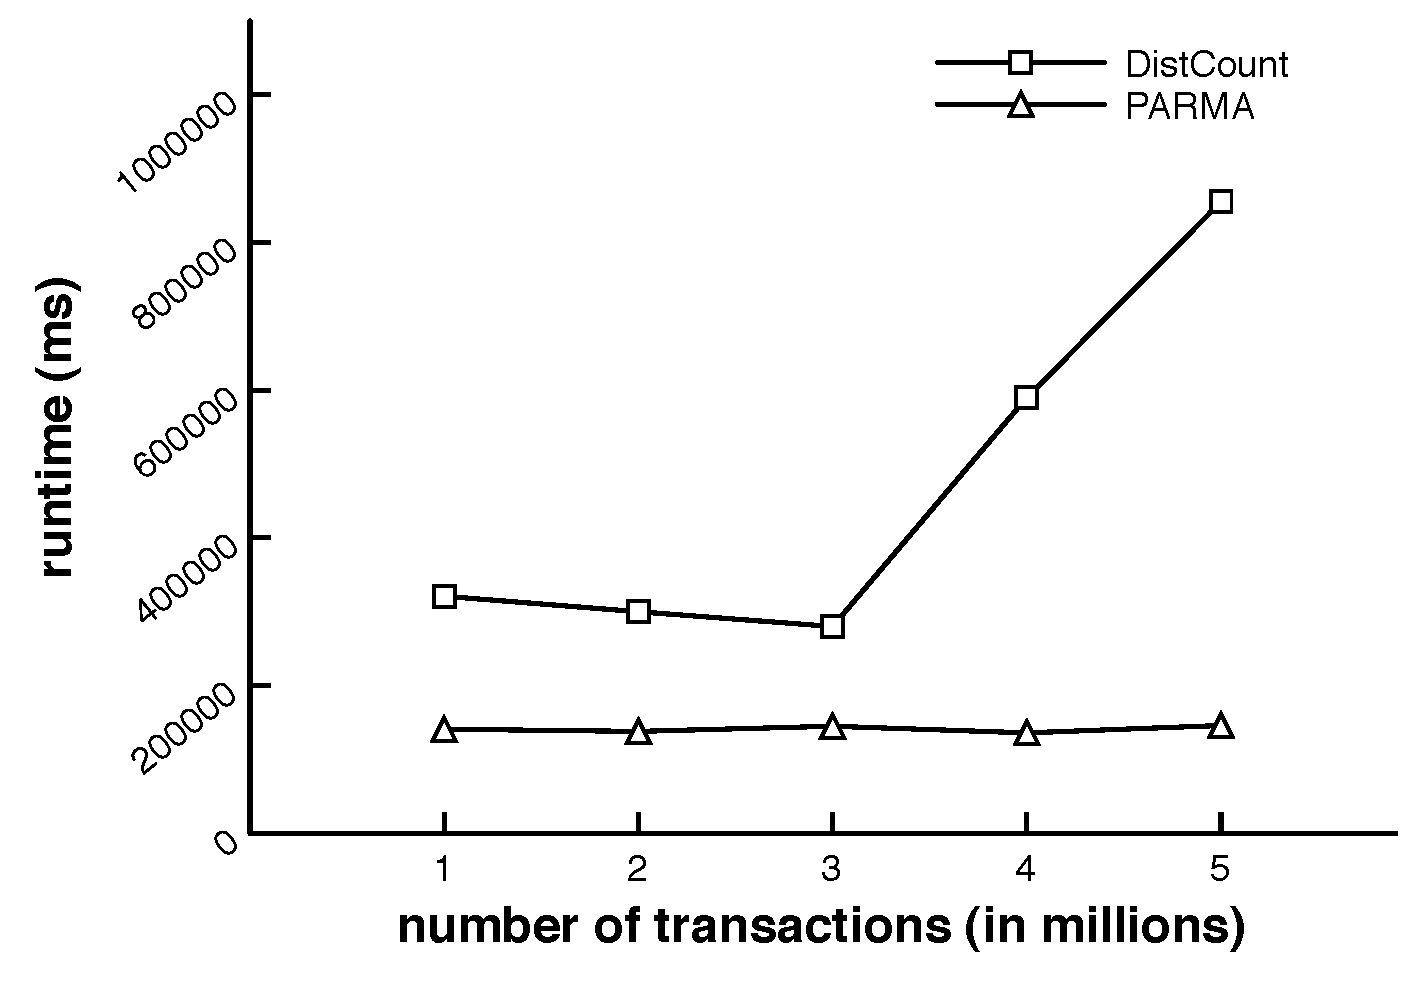
\includegraphics[width=0.49\textwidth]{parma/distributed_counting}
    \hfill
    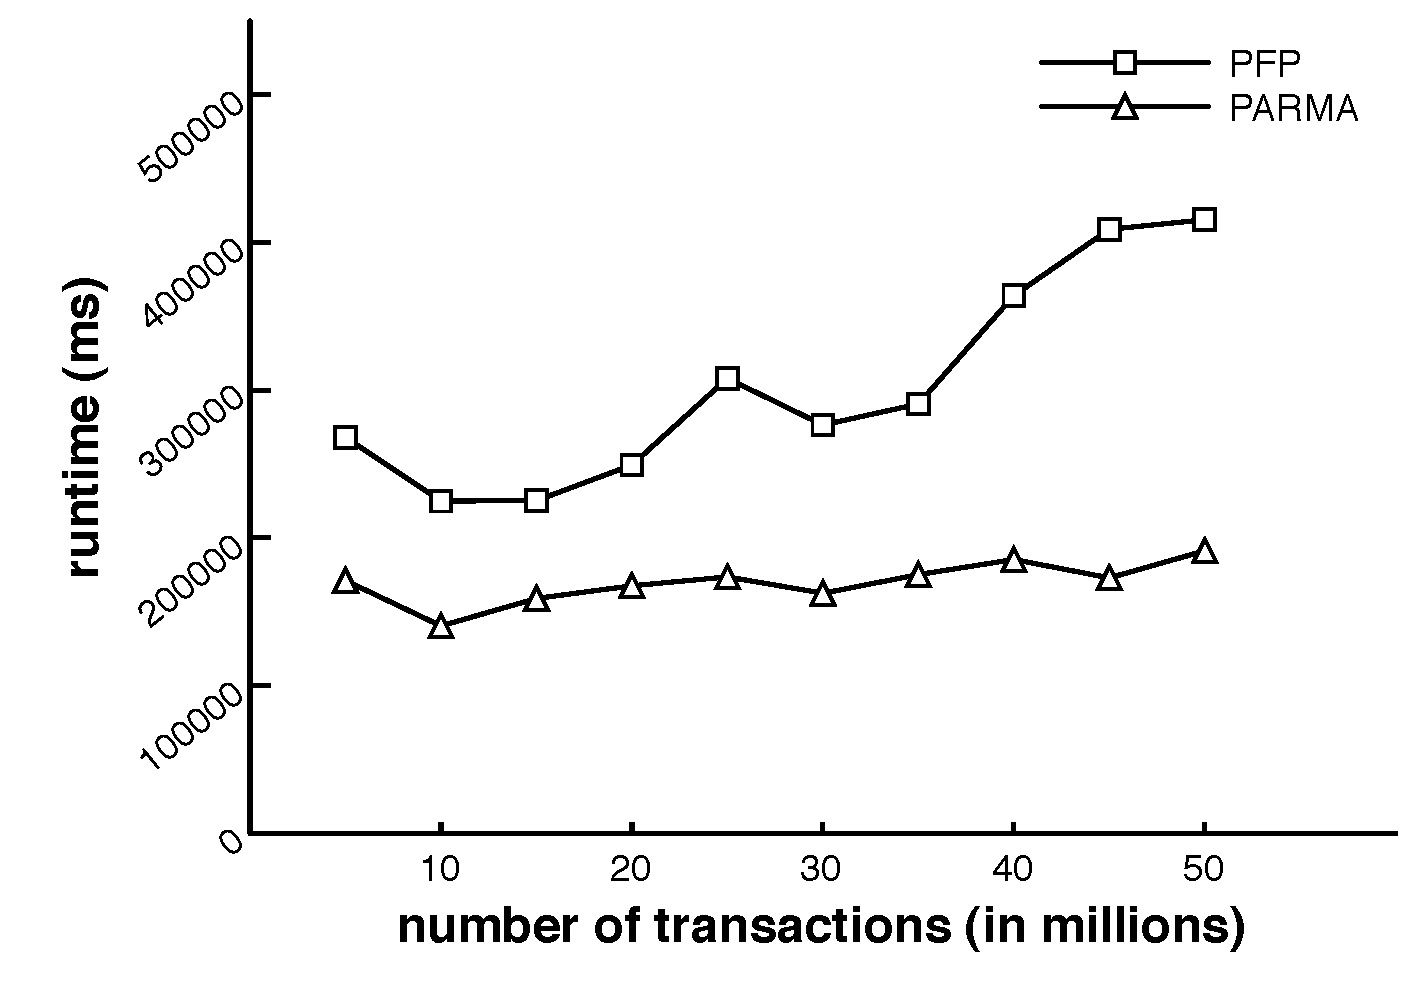
\includegraphics[width=0.49\textwidth]{parma/performance}
  \caption{A runtime comparison of PARMA with DistCount and PFP.}
\label{fig:parmaperformance}
\end{figure}

For the performance comparison with PFP, 10 datasets were generated
using parameter values from Table \ref{tab:param2} and ranging in size
from 10 to 50 million transactions.
The results are shown in
Figure~\ref{fig:parmaperformance} (bottom).
  For every dataset tested, PARMA was able
to mine the dataset roughly 30-55\% faster than PFP. The reason for the
relative performance advantage of PARMA is twofold. The first (and
primary) reason is that for larger datasets the size of the dataset that
PARMA has sampled (and mined) is staying the same, whereas PFP is mining
more and more transactions as the dataset grows. The second reason is
that as the dataset grows, PFP is potentially duplicating more and more
transactions as it assigns transactions to groups. A transaction that
belongs to multiple groups is sent to multiple reducers, resulting in
higher network costs.

The most important aspect of the comparison of PFP to PARMA is that the
runtimes as data grows are clearly diverging due to the reasons
discussed above. While 50 million transactions is very sizable, it is
not hard to imagine real-world datasets with transactions on the order
of billions. Indeed, many point-of-sale datasets would easily break this
boundary. In these scenarios a randomized algorithm such as PARMA would
show increasing performance advantages over exact algorithms such as any
of the standard non-parallel algorithms or PFP, which must mine the
entire dataset. At that scale, even transmitting that data over the
network (several times in the case of PFP) would become prohibitive.

To understand the performance of PARMA it is important to analyze the
runtimes at each of the various stages in the algorithm. To do this, we
have implemented runtime timers at very fine granularities throughout
our algorithm. The timers' values are written to Hadoop job logs for
analysis. This breakdown allows us to not only analyze the overall
runtime, but also the sections of the algorithm whose runtimes are
affected by an increase in data size. In Figure \ref{fig:parmabreakdown1}, a
breakdown of PARMA runtimes is shown for each of the six segments of the
algorithm, which include a map, shuffle and reduce phase for each of the
two stages. 
Due to space limitations, we only show the breakdown for a subset of
the datasets we tested. We observed the same patterns for all datasets.
This breakdown demonstrates several interesting aspects of
PARMA. First, the cost of the mining local frequent itemsets (stage 1,
reduce) is relatively constant. For many frequent itemset mining
implementations, this cost will grow with the size of the input. This is
not the case in PARMA, because local frequent itemset mining is being
done on constant-sized sample of the input. Indeed another interesting
observation, as expected, is that the only cost that increases as sample
size increases is the cost of sampling (stage 1, map). This is because
in order to be sampled the input data must be read, so larger input data
means larger read times. In practice, this cost is minimal and
grows linearly with the input, hence it will never be prohibitive,
especially considering all other current algorithms must read the entire
input data at least once, and in many cases multiple times. 

There is one outlier in the graph, which is the dataset with 5 million
transactions. Because each dataset was independently generated, it is
possible for a dataset to have a larger number of frequent itemsets than
other datasets, even if it has less transactions. This is the case with
the 5 million transaction dataset, which takes longer to run mine for both PARMA and PFP
due to the relatively greater number of frequent itemsets. 

\begin{comment}
To see that this is indeed what is
happening, we refer again to Figure \ref{fig:parmabreakdown1}. As expected,
the sample generation phase (stage 1, map) is smaller relative to the
larger datasets. However, the local frequent itemset mining phase (stage
1, reduce) is longer than any of the larger datasets. This is because
there are more frequent itemsets in that dataset. This can also be seen
in the relatively larger shuffle phase of stage 2, which is in charge of
sending all equivalent local frequent itemsets to the same reducer for
aggregation. Because there are more local itemsets present, this shuffle
stage is larger than for the other datasets. Because the same dataset
was used for the runtime of analysis of PFP and PARMA, and the overall
runtimes of both should increase in a dataset with more frequent
itemsets, we should see a higher runtime on the 5 million transaction
dataset for PFP relative to its the other datasets, which is indeed the
case. The runtime of PFP increases with both the size of the dataset as
well as the number of frequent itemsets present, but it is not until a
dataset of 25 million transactions that the runtime exceeds the runtime
for the 5 million transaction dataset. This outlier is not a flaw with
PARMA or PFP, but is a result of one of the inherent aspects of frequent
itemset mining: it takes longer to mine datasets with more frequent
itemsets.
\end{comment}

\begin{figure}[htb]
\centering
    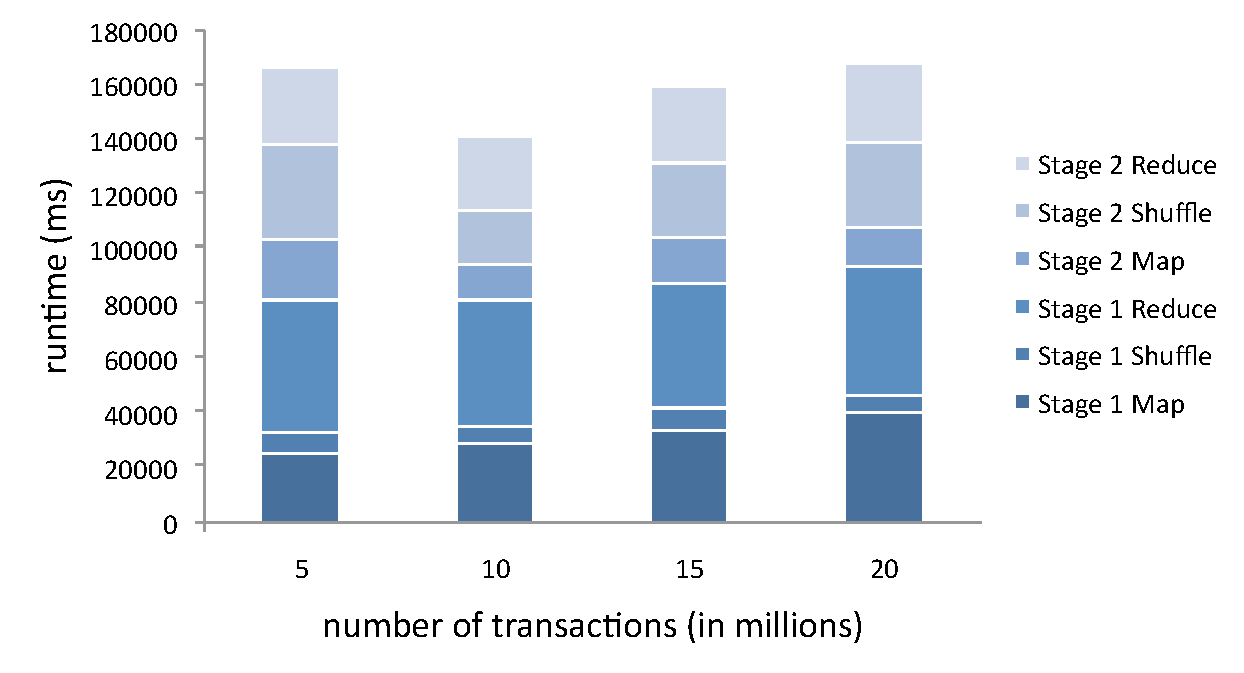
\includegraphics[width=0.75\textwidth]{parma/breakdown1}
  \caption{A comparison of runtimes of the map/reduce/shuffle phases
of PARMA, as a function of number of transactions. Run on
an 8 node Elastic MapReduce cluster.}
\label{fig:parmabreakdown1}
\end{figure}

\begin{figure}[htb]
  \centering
    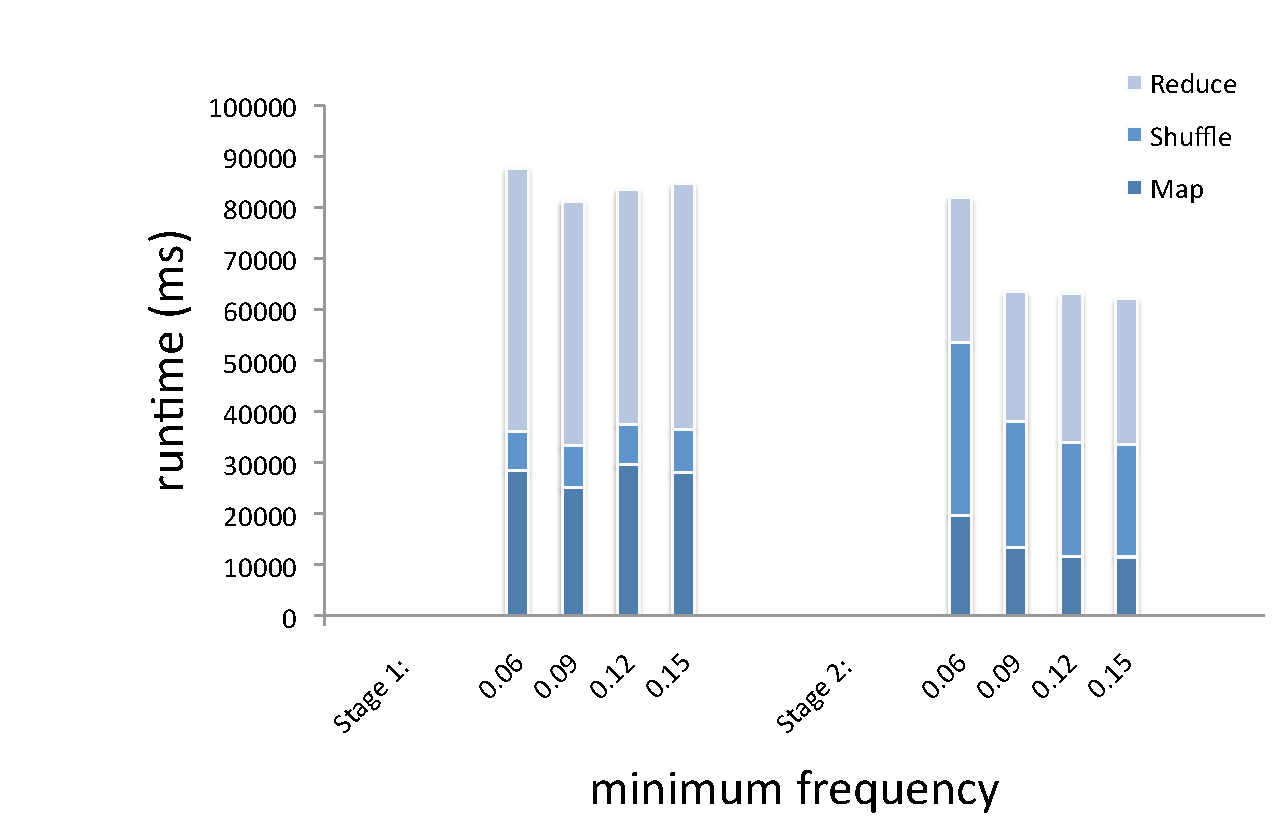
\includegraphics[width=0.75\textwidth]{parma/frequency}
  \caption{A comparison of runtimes of the map/reduce/shuffle phases
of PARMA, as a function of minimum frequency. Clustered by stage. Run
on an 8 node Elastic MapReduce cluster.}
\label{fig:parmafrequency}
\end{figure}

\begin{comment}
In Figure \ref{fig:parmabreakdown2}, a breakdown of total runtimes is shown
clustered by stage. In this view, it is apparent that most of the
phases of the algorithm are nearly constant across data sizes. The
obvious increase is the map of stage 1, which was discussed
above. Another slight runtime increase as data increases occurs in the
shuffle phase of stage 2. Because there are more transactions in the
larger datasets, there will be more frequent itemsets on average. In
stage 2, an identity mapper sends each frequent itemset to the
appropriate reducer for counting. Thus, all this data is being moved
across the network, which is manifested in the shuffle phase of stage
2. The more frequent itemsets, the more data there is to shuffle
across the network, which results in longer runtimes. Also, in
Figure~\ref{fig:parmabreakdown2} we once again notice that the 5 million
transaction dataset is an outlier. The longer than expected phase is
the shuffle phase of stage 2, which again suggests that this dataset
took longer to mine because more frequent itemsets were found.
\begin{figure}[htb]
  \centering
    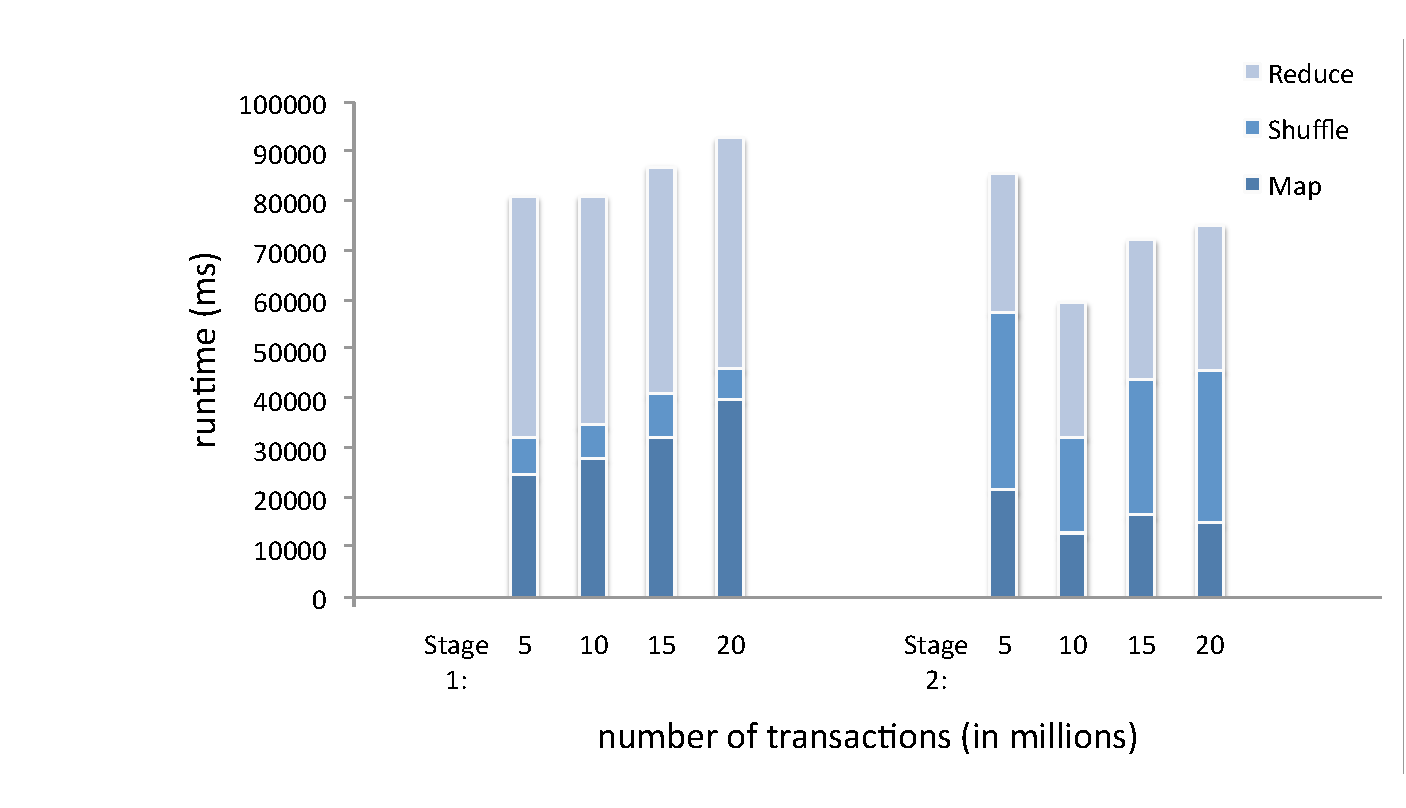
\includegraphics[width=0.4\textwidth]{breakdown2}
  \caption{A Comparison of runtimes of the map/reduce/shuffle phases
of PARMA, as a function of input dataset size. Clustered by stage. Run
on an 8 node Elastic MapReduce cluster.}
\label{fig:parmabreakdown2}
\end{figure}
\end{comment}

Figure \ref{fig:parmafrequency} shows the breakdown of PARMA runtimes as
the minimum frequency at which the data is mined at is changed. Data
size was kept constant at 10 million transactions. Minimum frequency
is used by the local frequent itemset mining algorithm to prune
itemsets; itemsets below the minimum frequency are not considered
frequent, nor is any superset since a superset must, by definition,
contain the not frequent set and therefore cannot be frequent
itself. Intuitively, a lower minimum frequency will mean more frequent
itemsets are produced. Other than a runtime increase in the local
frequent itemset mining phase (stage 1, reduce), the effects of this
can be seen in the stage 2 shuffle phase as well, as there is more
data to move across the network. Still, the added costs of mining with
lower frequencies are relatively small.

%\vspace{-10pt}
\subsection{Speedup and scalability}
To show the speedup of PARMA, we used a two-nodes cluster as the
baseline. Because PARMA is intended to be a parallel algorithm, the choice of a
two-nodes cluster was more appropriate than the standard single node
baseline. For the dataset, we used a 10 million transaction database
generated using the parameters in Table \ref{tab:param2}. The results
are shown in Figure \ref{fig:parmaspeedup}. The three lines on this graph
represent the relative speedup of both stage 1 and stage 2 as well as
the overall PARMA algorithm. The graph indicates that stage 1 is highly
parallelizable and follows a near-ideal speedup for up to 8 nodes,
after which a slight degradation of speedup occurs. There are two
reasons for this slight degradation. In the map phase of stage 1, due
to an implementation decision in Hadoop, the smallest unit of data
that can be split is one HDFS block. As we continue to add more nodes
to the cluster, we may have more available map slots than HDFS data
blocks, resulting in some slots being unused. Theoretically, this
could be fixed by allowing smaller granularity splitting in
Hadoop. Another cause of the slightly sub-ideal speedup in stage 1 is
from the reducer. Because the data in this experiment was held
constant, the slight degradation in speedup as more than 8 nodes were
added was a result of an inefficient over-splitting of transaction
data. If each reducer in stage 1 is mining a very small subset of the
transactions, the overhead of building the FP-tree begins to dominate
the cost of mining the FP-tree. This is because the cost of mining the
FP-tree is relatively fixed. Thus, we can ``over-split'' the data by
forcing the reducer to build a large FP-tree only to mine a small set
of transactions. For larger samples, the size of the cluster where
speedup degradation begins to occur would also increase, meaning PARMA
would continue to scale.

\begin{figure}[thb]
  \centering
  \begin{subfigure}[b]{0.49\textwidth}
    \centering
    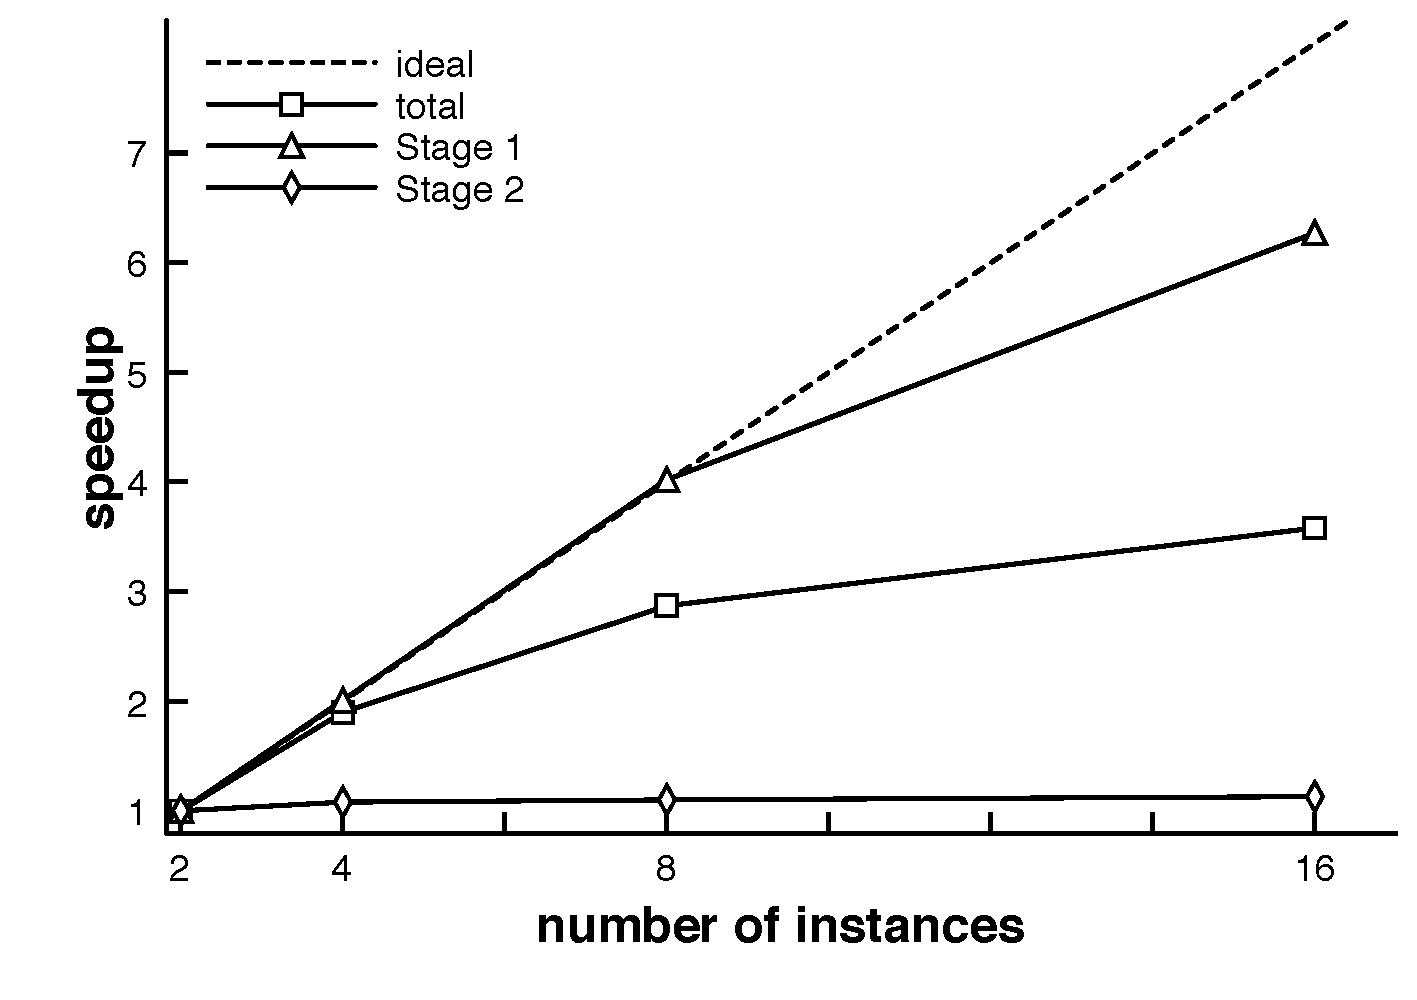
\includegraphics[width=\textwidth]{parma/speedup}
    \caption{Speedup analysis broken down by stages.}
    \label{fig:parmaspeedup}
  \end{subfigure}
  \hfill
  \begin{subfigure}[b]{0.49\textwidth}
    \centering
    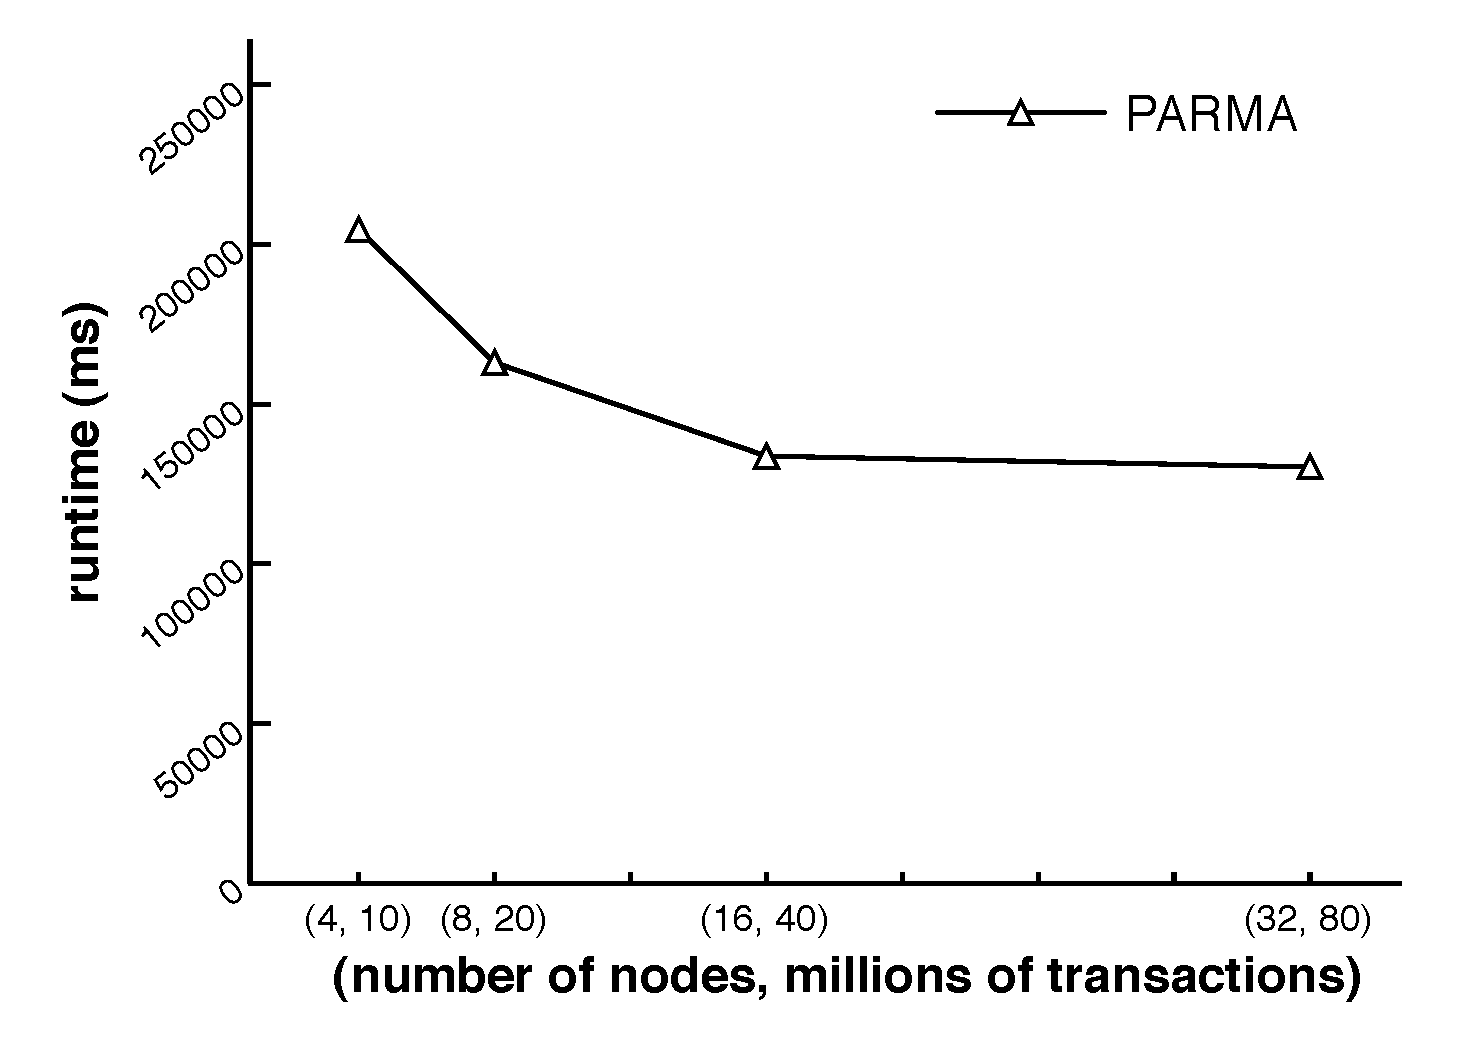
\includegraphics[width=\textwidth]{parma/scalability}
    \caption{Scalability as both data and cluster size are increased.}
    \label{fig:parmascalability}
  \end{subfigure}
  \caption{Speedup and scalability.}
\end{figure}

Also, as is clearly visible in the graph, the sub-ideal overall
speedup is due largely to the poor speedup of stage 2. Stage 2 is
bound almost entirely by the communication costs of transmitting the
local frequent itemsets from stage 1 to the reducers that will do the
aggregation. Because the amount of local frequent itemsets does not
change as more nodes are added, the communication for this stage does
not change. What does change is the number of itemsets each node must
aggregate. During the reduce phase, each node is assigned a set of
keys. All key/value pairs emitted from the map phase are sent to the
reducer assigned their respective key. The reducer is in charge of
aggregating the values and emitting one aggregate value per key assigned
to it. As more reducers are added to the cluster, each reducer will
have fewer keys assigned to it, and therefore must aggregate across
fewer values, resulting in faster aggregation. The small but existent positive
change in the line for stage 2 is a result of this slight speedup of the reduce
phase. 

Figure \ref{fig:parmascalability} depicts the scalability of PARMA as both
the size of the dataset (i.e. number of transactions) and the number of
nodes in the cluster are increased. The data and nodes are scaled
proportionally so that the ratio of data to nodes remains constant
across all experiments. This result shows that as nodes and data are
increased proportionally, the total runtime actually begins to decrease
for larger datasets. This is because as nodes are added to the cluster, the runtime of
the Stage 1 reducer (FIM) is decreased while the relative costs of
the Stage 1 mapper and Stage 2 remain the same. There is a leveling
off of the runtime between the 40M and 80M datasets, which can be
explained using Amdhal's law; because only portions of the algorithm
are parallelizable, there is a theoretical maximum speedup that is
possible. Still, the constant runtime as data is increased
demonstrates PARMA's potential scalability to real-world cluster and
dataset sizes. 

A very important aspect of PARMA that should be stressed again
here is that the size of the sample that will be mined does not depend
directly on size of the original database, but instead on the
confidence parameters $\varepsilon$ and $\delta$. From a practical
perspective, this means that assuming confidence parameters are
unchanged, larger and larger datasets can be mined with very little
increase in overall runtime (the added cost will only be the extra
time spent reading the larger dataset initially during
sampling). Because of this, clusters do not need to scale
with the data, and often a relatively modest cluster size will be
able to mine itemsets in a very reasonable time. 

\subsection{Accuracy}
The output of PARMA is a collection of frequent itemsets which approximates the
collection one can obtain by mining the entire dataset. Although our analysis
shows that PARMA offers solid guarantees in terms of accuracy of the output, we
conducted an extensive evaluation to assess the actual performances of PARMA in
practice, especially in relation to what can be analytically proved.

We compared the results obtained by PARMA with the exact collection of
itemsets from the entire dataset, for different values of the parameters
$\varepsilon$, $\delta$, and $\theta$, and for different datasets. A first important
result is that in all the runs, the collection computed by PARMA was indeed an
absolute $\varepsilon$-close approximation to the real one, i.e., all the properties from
Definition~\ref{def:parmaeapproxfi} were satisfied. This fact suggests that the confidence in
the result obtained by PARMA is actually greater than the level $1-\delta$
suggested by the analysis. This can be explained by considering that we had to
use potentially loose theoretical bounds in the analysis to make it tractable. 

Given that all real frequent itemsets were included in the output, we then
focused on how many itemsets with real frequency in the interval
$[\theta-\varepsilon,\theta)$ were included in the output. It is important to
notice that these itemsets would be \emph{acceptable} false positives, as
Definition~\ref{def:parmaeapproxfi} does not forbid them to be present in the output.
We stress again that the output of PARMA never contained \emph{non-acceptable}
false positives, i.e. itemsets with real frequency less than the minimum
frequency threshold $\theta$. The number of acceptable false positives included in the
output of PARMA depends on the distribution of the real frequencies in the
interval $[\theta-\varepsilon,\theta)$, so it should not be judged in absolute
terms. In Table~\ref{tab:falsepositives} we report, for various values of
$\theta$, the number of real frequent itemsets (i.e., with real frequency at
least $\theta$, the number of acceptable false positives (AFP) contained in the output
of PARMA, and the number of itemsets with real frequency in the interval
$[\theta-\varepsilon,\theta)$, i.e., the maximum number of acceptable false
positives that may be contained in the output of PARMA (Max AFP). These numbers
refers to a run of PARMA on (samples of) the 10M dataset, with
$\varepsilon=0.05$ and $\delta=0.01$. It is evident that PARMA does a very good
job in filtering out even acceptable false positives, especially at lower
frequencies, when their number increases. This is thanks to the fact that  an
itemset is included in the output of PARMA if and only if it appears in the
majority of the collections obtained in the first stage. Itemsets with real frequencies
in $[\theta-\varepsilon,\theta)$ are not very likely to be contained in many of
these collections.

\begin{table}
  \centering
  \begin{tabular}{cccc}
    \hline
    $\theta$ & Real FI's & Output AFP's & Max AFP's \\
    \hline
    $0.06$ & 11016 & 11797 & 201636 \\
    $0.09$ & 2116& 4216& 10723 \\
    $0.12$ & 1367& 335& 1452\\
    $0.15$ & 1053& 299& 415\\
    \hline
  \end{tabular}
  \caption{Acceptable False Positives in the output of PARMA}
  \label{tab:falsepositives}
\end{table}

We conducted an evaluation of the accuracy of two other components of the
output of PARMA, namely the estimated frequencies for the itemsets in the output
and the width of the confidence bounds for these estimations. In
Figure~\ref{fig:parmaabsfreqerr} we show the distribution of the absolute error in
the estimation, i.e. $|\tilde{f}(X)-f_\Ds(X)|$ for all itemsets $X$ in the
output of PARMA, as $\theta$ varies. The lower end of the ``whisker'' indicates the minimum error,
the lower bound of the box corresponds to the first quartile, the segment across
the box to the median, and the upper bound of the box to the third quartile. The
top end of the whisker indicates the maximum error, and the central diamond
shows the mean. This figure (and also Figure~\ref{fig:parmaconfintwidth}) shows the values
for a run of PARMA on samples of the 10M dataset, with $\varepsilon=0.05$ and
$\delta=0.01$. We can see that even the maximum values are one order of
magnitude smaller than the threshold of $0.05$ guaranteed by the analysis, and
many of the errors are two or more orders of magnitude smaller. It is also
possible to appreciate that the distribution of the error would be heavily concentrated in a
small interval if the maximum error were not so high, effectively an outlier.
The fact that the average and the median of the error, together with the entire ``box'' move down as the
minimum frequency threshold decrease can be explained by the fact that at lower
frequencies more itemsets are considered, and this makes the distribution less
susceptible to outliers. Not only this is a sign of the high level of accuracy
achieved by PARMA, but also of its being consistently accurate on
a very large portion of the output.

\begin{figure}[htb]
 \centering
    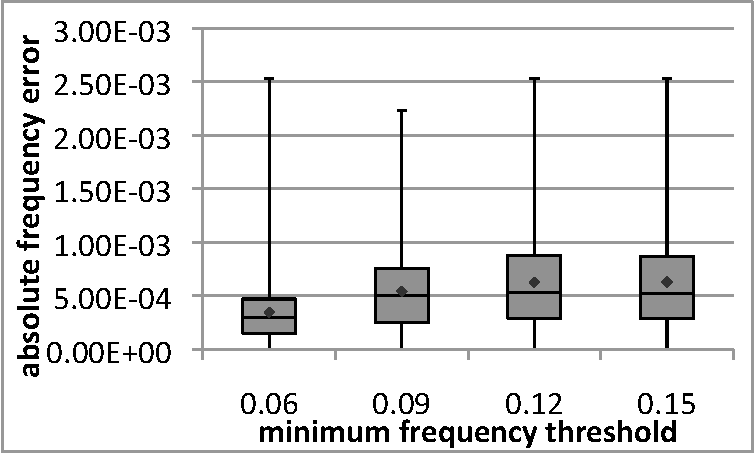
\includegraphics[width=0.75\textwidth]{parma/absfreqerr}
  \caption{Error in frequency estimations as frequency varies.}
  \label{fig:parmaabsfreqerr}
\end{figure}

\begin{figure}[htb]
 \centering
    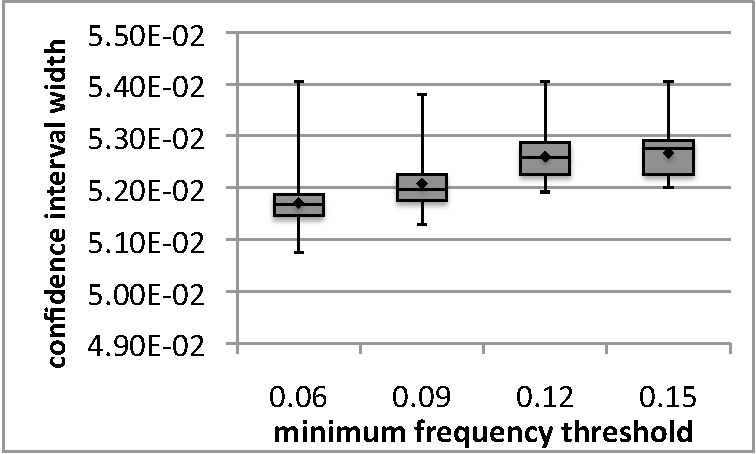
\includegraphics[width=0.75\textwidth]{parma/confintwidth}
  \caption{Width of the confidence intervals as frequency varies.}
  \label{fig:parmaconfintwidth}
\end{figure}

Finally, in Figure~\ref{fig:parmaconfintwidth} we show the distribution of the widths
of the confidence intervals $\mathcal{K}(A)$ for the frequency estimations
$\tilde{f}(A)$ of the itemsets $A$ in the output of PARMA. Given that
$\varepsilon=0.05$, the maximum allowed width was $2\varepsilon=0.1$. It is
evident from the figures that PARMA returns much narrower intervals, of size almost
$\varepsilon$. Moreover, the distribution of the width is very concentrated, as
shown by the small height of the boxes, suggesting that PARMA is extremely
consistent in giving very high quality confidence intervals for the estimations.
We state again that in all runs of PARMA in our tests, all the confidence
intervals contained the estimation and the real frequency, as requested by
Definition~\ref{def:parmaeapproxfi}. As seen in the case of the estimation
error, the distribution of the widths shifts down at lower thresholds $\theta$.
This is motivated by the higher number of itemsets in the output of PARMA at
those frequencies. Their presence makes the distribution more robust to
outliers. We can conclude that PARMA gives very narrow but
extremely accurate confidence intervals across the entirety of its output.

This analysis of the accuracy of various aspects of PARMA's output shows that
PARMA can be very useful in practice, and the confidence of the end user in
the collections of itemsets and estimations given in its output can be even higher
than what is guaranteed by the analysis.


\section{Conclusions}
\label{sec:parmaconc}

In this paper, we have described PARMA, a parallel algorithm for mining
quasi-optimal collections of frequent itemsets and association rules in MapReduce.
We showed through theoretical analysis that PARMA offers provable guarantees on
the quality of the output collections. Through experimentation on a wide range
of datasets ranging in size from 5 million to 50 million transactions,
we have demonstrated a 30-55\% runtime improvement over PFP, the
current state-of-the-art in exact parallel mining algorithms on MapReduce.
Empirically we were able to verify the accuracy of the theoretical bounds, as
well as show that in practice our results are orders of magnitude more accurate
than is analytically guaranteed. Thus PARMA is an algorithm that can scale to
arbitrary data sizes while simultaneously providing nearly perfect results. 

\section{Acknowledgments}
\label{sec:parmaack}
The work of Riondato, DeBrabant, and Upfal was supported in part by NSF award IIS-0905553.


%\bibliographystyle{abbrv}
%\bibliography{fim,mrfim,mr} 
\iffalse
\begin{thebibliography}{10}
\begin{small}

\vspace{7pt}
\bibitem{AgrawalIS93}
R.~Agrawal, T.~Imieli\'{n}ski, and A.~Swami.
\newblock Mining association rules between sets of items in large databases.
\newblock SIGMOD '93.

\bibitem{AgrawalS94}
R.~Agrawal and R.~Srikant.
\newblock Fast algorithms for mining association rules in large databases.
\newblock VLDB '94.

\bibitem{Mahout}
{Apache Mahout}.
\newblock \url{http://mahout.apache.org/}.

\bibitem{BuehrerPTKS07}
G.~Buehrer, S.~Parthasarathy, S.~Tatikonda, T.~Kurc, and J.~Saltz.
\newblock Toward terabyte pattern mining: an architecture-conscious solution.
\newblock PPoPP '07.

\bibitem{ChierichettiKT10}
F.~Chierichetti, R.~Kumar, and A.~Tomkins.
\newblock Max-cover in {Map-Reduce}.
\newblock WWW '10.

\bibitem{ChuKLYBNO06}
C.-T. Chu, S.~K. Kim, Y.-A. Lin, Y.~Yu, G.~R. Bradski, A.~Y. Ng, and
  K.~Olukotun.
\newblock {Map-Reduce} for machine learning on multicore.
\newblock NIPS '06.

\bibitem{Fp}
F.~Coenen.
%\newblock The {LUCS-KDD FP}-growth association rule mining algorithm.
\newblock
\url{http://www.cxc.liv.ac.uk/~frans/KDD/Software/FPgrowth/fpGrowth.html}

\bibitem{CongHHP05}
S.~Cong, J.~Han, J.~Hoeflinger, D.~Padua.
\newblock A sampling-based framework for parallel data mining.
\newblock PPoPP '05.

\bibitem{ARTool}
L.~Cristofor.
\newblock {ART}ool.
\newblock \url{http://www.cs.umb.edu/~laur/ARtool/}, 2006.

\bibitem{CryansRC10}
J.-D. Cryans, S.~Ratt{\'e}, and R.~Champagne.
\newblock Adaptation of {APriori} to {MapReduce} to build a warehouse of
  relations between named entities across the web.
\newblock DBKDA '10.

\bibitem{DeanG08}
J.~Dean and S.~Ghemawat.
\newblock {MapReduce}: Simplified data processing on large clusters.
\newblock {\em CACM}, 51(1):107--113, 2008.

\bibitem{EHZaiane06}
M.~El-Hajj and O.~Zaiane.
\newblock Parallel leap: large-scale maximal pattern mining in a distributed
  environment.
\newblock ICPADS '06.

\bibitem{FangEtAl08}
W.~Fang, K.~K. Lau, M.~Lu, X.~Xiao, C.~K. Lam, Y.~Yang, B.~He, Q.~Luo, P.~V.
  Sander, and K.~Yang.
\newblock Parallel data mining on graphics processors.
\newblock Technical Report~07, The Hong Kong University of Science {\&}
  Technology, 2008.

\bibitem{GhotingKPK11}
A.~Ghoting, P.~Kambadur, E.~Pednault, and R.~Kannan.
\newblock {NIMBLE}: a toolkit for the implementation of parallel data mining
and machine learning algorithms on {MapReduce}.
\newblock KDD '11.

\bibitem{GoodrichSZ11}
M.~T. Goodrich, N.~Sitchinava, and Q.~Zhang.
\newblock Sorting, searching, and simulation in the {MapReduce} framework.
\newblock {\em CoRR}, abs/1101.1902, 2011.

\bibitem{Hammoud11}
S.~Hammoud.
\newblock {\em MapReduce Network Enabled Algorithms for Classification Based on
  Association Rules}.
\newblock PhD thesis, Brunel University, 2011.

\bibitem{HanPY00}
J.~Han, J.~Pei, and Y.~Yin.
\newblock Mining frequent patterns without candidate generation.
\newblock {\em SIGMOD Rec.}, 29:1--12, May 2000.

\bibitem{LiWZZC08}
H.~Li, Y.~Wang, D.~Zhang, M.~Zhang, and E.~Y. Chang.
\newblock {PFP}: Parallel {FP-G}rowth for query recommendation.
\newblock RecSys '08.

\bibitem{LiZ11}
L.~Li and M.~Zhang.
\newblock The strategy of mining association rule based on cloud computing.
\newblock BCGIN '11.

\bibitem{LiG04}
Y.~Li and R.~Gopalan.
\newblock Effective sampling for mining association rules.
\newblock AI '04.

\bibitem{LinS10}
J.~Lin and M.~Schatz.
\newblock Design patterns for efficient graph algorithms in MapReduce.
\newblock  MLG '10.

\bibitem{LiuLZT07}
L.~Liu, E.~Li, Y.~Zhang, Z.~Tang.
\newblock Optimization of frequent itemset mining on multiple-core processor.
\newblock VLDB '07.

\bibitem{MannilaTV94}
H.~Mannila, H.~Toivonen, and I.~Verkamo.
\newblock Efficient algorithms for discovering association rules.
\newblock KDD '94.

\bibitem{MitzenmacherU05}
M.~Mitzenmacher and E.~Upfal.
\newblock {\em Probability and computing}.
\newblock Cambridge University Press, 2005.

\bibitem{OzkuralUA11}
E.~Ozkural, B.~Ucar, and C.~Aykanat.
\newblock Parallel frequent item set mining with selective item replication.
\newblock {\em IEEE Trans. on Paral. and Distrib. Sys.},
  22(10):1632--1640, 2011.

\bibitem{Parthasarathy02}
S.~Parthasarathy.
\newblock Efficient progressive sampling for association rules.
\newblock ICDM '02.

\bibitem{PietracaprinaPRSU11}
A.~Pietracaprina, G.~Pucci, M.~Riondato, F.~Silvestri, and E.~Upfal.
\newblock Space-round tradeoffs for {MapReduce} computations.
\newblock ICS' 12. 

\bibitem{PietracaprinaRUV10}
A.~Pietracaprina, M.~Riondato, E.~Upfal, and F.~Vandin.
\newblock Mining top-{K} frequent itemsets through progressive sampling.
\newblock {\em Data Min.~and Knowl.~Disc}, 21:310--326, 2010.

\bibitem{RiondatoU11}
M.~Riondato and E.~Upfal.
\newblock Efficient discovery of association rules and frequent itemsets
  through sampling with tight performance guarantees.
\newblock {\em CoRR}, abs/1111.6937v3, 2012.

\bibitem{JinYA05}
J.~Ruoming, Y.~Ge, and G.~Agrawal.
\newblock Shared memory parallelization of data mining algorithms: techniques,
  programming interface, and performance.
\newblock {\em IEEE Trans. on Knowl. and Data Engin.}, 17(1):71--89, 2005.

\bibitem{baron}
N.~V. Sahinidis and M.~Tawarmalani.
\newblock {\em {BARON 9.0.4: Global Optimization of Mixed-Integer Nonlinear
  Programs, {\em User's Manual}}}, 2010.

\bibitem{Toivonen96}
H.~Toivonen.
\newblock Sampling large databases for association rules.
\newblock VLDB '96.

\bibitem{YangLF10}
X.~Y. Yang, Z.~Liu, and Y.~Fu.
\newblock {MapReduce} as a programming model for association rules algorithm on
  {Hadoop}.
\newblock ICIS '10.

\bibitem{Zaki99}
M.~Zaki.
\newblock Parallel and distributed association mining: a survey.
\newblock {\em IEEE Concurrency}, 7(4):14 --25, 1999.

\bibitem{ZakiPLO97}
M.~Zaki, S.~Parthasarathy, W.~Li, and M.~Ogihara.
\newblock Evaluation of sampling for data mining of association rules.
\newblock RIDE '97.

\bibitem{ZhouZCLF10}
L.~Zhou, Z.~Zhong, J.~Chang, J.~Li, J.~Huang, and S.~Feng.
\newblock Balanced parallel {FP-Growth} with {MapReduce}.
\newblock YC-ICT '10.

\end{small}
\end{thebibliography}
\fi


%\chapter{A progressive sampling algorithm for efficiently mining frequent
itemsets and association rules}\label{ch:shatterfi}
\chaptermark{Mining frequent itemsets through progressive sampling}

In this chapter we will present an algorithm based on progressive sampling to
extract an approximate collection of the frequent itemsets from a very large
dataset. For an introduction to the problem of frequent itemsets mining, see
Section~\ref{sec:preldm}.

In the setting of frequent itemsets mining, progressive sampling algorithms work
by starting from a small random sample of the dataset, checking for some
condition (stopping rule) which may or may not require the extraction of
frequent itemsets from the sample, and accordingly decide whether to stop and
return the collection of frequent itemsets from the sample or compute a larger
sample according to a predefined or dynamic sample size schedule.

The main issue in developing progressive sampling algorithms is the definition
of the stopping rule. Ideally, it should be efficient to evaluate and it should
suggest to stop the process as soon as possible. Moreover, it should be such
that the collection of frequent itemsets extracted from the last sample should
offer some quality guarantees in order to be a good approximation of the
original collection. 
It is not easy to develop a stopping rule achieving all these goals, and indeed
many stopping rules in the literature do not succeed. They either
require an expensive mining of frequent itemsets from the current
sample, do not offer guarantees on the quality of the approximation, or
both~\citep{BronnimanCDHS03,ChandraB11,ChenHH11,ChenHS02,ChuangCY05,HuY06,HwangK06,JiaG05,MahafzahABAZ09,Parthasarathy02,PietracaprinaRUV10,SchefferW02,WangDC05}.
This is due to the fact that most of them compare the frequencies of the
itemsets in the current sample with those from the previous sample, in order to
understand whether they are converging to their expectations, i.e., to their
frequencies in the dataset. In terms of the sample schedule, \citet{JohnL96}
showed that a geometrically increasing sample schedule is optimal up to a
constant factor.

Our goal is to develop a stopping rule that satisfies all the three goals
mentioned before and potentially an adaptive sampling schedule based on the
stopping rule that can, if not provably, at least experimentally achieve a
stopping sample size smaller than that suggested by the geometric schedule.
The algorithm will not need to mine the frequent itemsets from the current
sample in order to evaluate the stopping rule. To develop and analyze our
stopping rule, we will use \emph{data-dependent bounds} on the deviations of all
the frequencies in the sample from their real values. These bounds, based on
\emph{Rademacher averages} are a recent development in statistical learning
theory~\citep{BoucheronBL05,Kaariainen04,KaariainenME04,KoltchinskiiAADP00,Koltchniskii01}
and have already been successfully employed in a progressive sampling algorithm
for a different problem~\citep{ElomaaK02}. We believe the practicality of these
bounds has not been fully exploited yet. The major difficulty in using these
bounds is the development of an easy-to-compute upper bound to a characteristic
combinatorial quantity of the sample. This upper bound is known as the
\emph{Vapnik-Chervonenkis shatter
coefficient}~\citep{BoucheronBL05,DevroyeGL96}. From an initial study, we
believe that the VC shatter coefficient for the problem at hand will depend on
the distribution of the lengths of the transactions in the sample. We already
saw in Chapter~\ref{ch:vcmine} that the VC-dimension of a dataset is 
bounded above by a quantity, the d-index, that depends on the
distribution of lengths of the longest transactions in the dataset. This,
together with other insights based on the definition of VC shatter coefficient
give us reasons to believe that the ``right'' bound should depend on the entire
distribution. We will conduct an extensive experimental evaluation of our
algorithms on real and artificial dataset, comparing its performances with other
progressive and static sampling algorithms.


\chapter{Controlling false positives in frequent itemsets mining through the
VC-dimension}\label{ch:realfis}
\chaptermark{False positives in frequent itemsets mining}
%\begin{abstract} \small\baselineskip=9pt
   Frequent Itemsets (FIs) mining is a fundamental primitive in data mining. It
   requires to identify %that identifies 
   all itemsets appearing in at least a fraction %at least
   $\theta$ of a transactional dataset $\Ds$. Often though, the ultimate goal
   of mining $\Ds$ is not an analysis of the dataset \emph{per se}, but the
   understanding of the underlying process that generated it. %$\Ds$
   Specifically, in many applications $\Ds$ is a collection of samples obtained from an
   unknown probability distribution $\prob$ on transactions, and by extracting
   the FIs in $\Ds$ one attempts to infer itemsets that are
   frequently (i.e., with probability at least $\theta$) generated by $\prob$, which we call the True Frequent Itemsets
   (TFIs). Due to the inherently stochastic nature of the generative process, the
   set of FIs is only a rough approximation of the set of TFIs, as it %may contain
   often contains
   a huge number of \emph{false positives}, %spurious itemsets, 
   i.e., spurious itemsets that are not among the
   TFIs. In this work we design and analyze an algorithm %method 
   to identify a threshold $\hat{\theta}$ such that the collection of itemsets
   %of $\Ds$ 
   with frequency at least $\hat{\theta}$ in $\Ds$
   contains only TFIs with probability at least $1-\delta$, for
   some user-specified $\delta$. Our method uses %makes use of 
   results from statistical learning theory involving the (empirical) VC-dimension of the
   problem at hand. This allows us to identify %larger fraction of the TFIs
   almost all the TFIs without including any false positive. %(i.e., to achieve higher statistical power) 
   %than what could be done using traditional methods  %multiple hypothesis testing
   %corrections. 
   We also experimentally compare our method with the direct mining of $\Ds$ at
   frequency $\theta$ and with
   techniques based on widely-used standard bounds (i.e., the Chernoff bounds)
   of the binomial distribution, and show that our algorithm outperforms these methods and
   achieves even better results than what is guaranteed by the theoretical
   analysis.
   %s permits the identification of a very large fraction %subset of the TFIs, without reporting any false positive on real datasets.
   %while controlling the probability of reporting spurious itemsets.
     %This allows us to achieve, on the %same data, much stricter bounds
   %on the FWER than what could be done using
   %traditional multiple hypothesis testing corrections, or even using more
   %recent techniques as the hold-out. In our experimental evaluation we show
   %empirically that our test has very high statistical power, i.e., the output
   %collection contains a large fraction of the RFI's, while correctly bounding
   %the FWER.
 \end{abstract}

%{\bf Categories and Subject Descriptors:} H.2.8 [Database Management]: Database Applications -- \emph{Data Mining}

{\bf Keywords:} Frequent itemsets, VC-dimension, False positives,
Distribution-free methods, Frequency threshold identification.


%The extraction of association rules is one of the fundamental primitives in
%data mining and knowledge discovery from large databases~\citep{AgrawalIS93}.
%In its most general definition, the problem can be reduced to identifying
%frequent sets of items, or \emph{frequent itemsets}, appearing in at
%least a fraction  $\theta$ of all transactions in a dataset, where $\theta$ is provided in
%input by the user. Frequent itemsets and association rules are not only of
%interest for classic data mining applications (e.g., market basket analysis), but
%are also useful for further data analysis and mining task, including clustering,
%classification, and indexing~\citep{han2006data,HanCXY07}.

In this chapter we present the task of mining Frequent Itemsets (FIs) from a
different point of view, and show that we can use VC-dimension to avoid the
inclusion of \emph{false positives} in the results of mining. In most
applications, the set of FIs is not interesting \emph{per
se}. %
%one is not interested in mining a dataset to extract the
%frequent itemsets \emph{per se}. 
Instead, the mining results %process is 
are used to infer properties of the \emph{underlying process} that generated the
dataset. Consider for example the following scenario: a researcher would like %wants 
to identify frequent associations (i.e., itemsets) between preferences among
Facebook users. To this end, she sets up an online survey %on Facebook 
which is filled out by a \emph{small fraction} of Facebook users (some users may even
take the survey multiple times). Using this information, the researcher wants to
infer the associations (itemsets) that are frequent for the \emph{entire} Facebook
population. In fact, the %one can 
 whole Facebook population and the online survey define the underlying \emph{process} that
generated the dataset \emph{observed} by the researcher. We are
interested in answering the following question: %and ask 
how can we use the latter (the observed dataset) to identify itemsets that are
frequent in the former (the whole population)?
%from which the dataset observed by the researcher has been
%generated, and wants to use the latter to identify frequent itemsets in the
%former. 
This is a very natural question, as is the underlying assumption that the
observed dataset is \emph{representative} of the generating process. For
example, in market basket analysis, 
%Another example is given by market basket analysis: in this case 
%one uses the %current, 
the observed purchases of customers are used to infer the future
purchase habits %pattern 
of all customers while assuming that %in the future 
the purchase behavior that generated the dataset is representative of the one
that will be followed in the future.
%that generated the current dataset %will be followed).

A natural and general model to describe these concepts %settings 
is to assume that the transactions in the dataset $\Ds$ are \emph{independent
identically distributed} (i.i.d.) samples from an \emph{unknown} probability
distribution $\prob$ defined on all possible transactions built on a set of
items. %with items appearing in $\Ds$. %built on the sets of items appearing $\Ds$. 
Since $\prob$ is fixed, each itemset $A$ has a fixed \emph{probability} $\tfreq(A)$
to appear in a transaction sampled from $\prob$. We call $\tfreq(A)$ the
\emph{true frequency} of $A$ (w.r.t.~$\prob$). The true frequency corresponds
to the fraction of transactions that contain the itemset $A$ among an infinite
set %number 
of transactions. %, that contain the itemset $A$. % and each itemset has a fixed probability to appear in a random transaction from $\prob$. 
The real goal of the mining process is then to identify itemsets that have
true frequency $\tfreq$ at least $\theta$, i.e., the \emph{True Frequent
Itemsets} (TFIs). %to appear in a random transaction drawn from $\prob$, given that for an itemset such
%probability corresponds to the fraction of transactions, among an infinite
%number of transactions, that contain the itemset. 
In the market basket analysis example%above
, $\Ds$ contains %is 
the observed purchases of customers, the \emph{unknown} distribution $\prob$
describes the purchase behavior of the customers as a whole, and we want to
analyze $\Ds$ to find the itemsets that have probability (i.e., true frequency) %$\tfreq$ 
at least $\theta$ to be bought by a customer.

Since $\Ds$ represents only a \emph{finite} sample from $\prob$, the set $F$ of frequent itemsets
of $\Ds$ w.r.t.~$\theta$ %at threshold $\theta$ 
only provides an \emph{approximation} of the True Frequent Itemsets: %, and 
due to the stochastic nature of the generative process %the set 
$F$ %of frequent itemsets of $\Ds
may contain a number of \emph{false positives}, %\emph{spurious (or false) discoveries}
 i.e., itemsets that appear among the frequent itemsets of
 $\Ds$ but whose \emph{true} frequency is smaller than %are not generated with probability at least 
$\theta$. %, may be reported. 
At the same time, some itemsets with true frequency
greater than $\theta$ may have a frequency in $\Ds$ that is \emph{smaller} than
$\theta$ (\emph{false negatives}), and therefore not be in $F$. This implies
that %Given that $\prob$ is not known, on one hand 
one can not aim at identifying \emph{all and only} the itemsets having true frequency %probability 
at least $\theta$.
% in $\prob$.
Even worse, from the data analyst's point of view, % On the other hand, 
there is \emph{no guarantee or bound on the number of false positives} reported
in $F$. %the collection of frequent itemsets of $\Ds$ w.r.t.~$\theta$.
%using the frequent itemsets of $\Ds$ as a proxy for such itemsets does not
%provide any \emph{guarantee on the number of false discoveries}. %that are reported. 
Consider the following scenario as an example. Let $A$ and $B$ be two (disjoint)
sets of pairs of items. The set $A$ contains 1,000 disjoint pairs, while $B$
contains 10,000 disjoint pairs. Let $\prob$ be such that, for any pair $(a,a')\in
A$, we have $\tfreq((a,a'))=0.1$, and for any pair $(b,b')\in B$, we have
$\tfreq((b,b'))=0.09$. Let $\Ds$ be a dataset of 10,000 transactions sampled from
$\prob$. %For example, assume that %in $\prob$ 
%there are two sets $A$ and $B$ of pairs of items:
%the set $A$ of 1000 (disjoint) pairs of items with  probability 0.1 in $\prob$, and
%the set $B$ of 10000 (disjoint) pairs of items with probability 
%0.09 in $\prob$. Assume that all pairs are independent in $\prob$, and we have 
%a dataset $\Ds$ of 10000 transactions from $\prob$ .
%If 
We are interested in finding pairs of items that have true frequency at least %probability 
$\theta=0.095$. %in $\prob$, and
If we extract the pairs of items with frequency at least $\theta$ in $\Ds$,
it is easy to see that in expectation %around 
50 of the 1,000 pairs from $A$ will have frequency in $\Ds$ %appear in $\Ds$ with frequency
\emph{below} $0.095$, and in expectation %around 
400 pairs from $B$ will have frequency in $\Ds$ %appear in $\Ds$ with frequency 
\emph{above} $0.095$.
Therefore, the set of pairs that have frequency at least $\theta$ in $\Ds$ does
\emph{not} contain % are missing 
some of the pairs that have true frequency %probability 
at least $\theta$ %in $\prob$ 
(false negatives), but %and also 
includes a huge number of %some 
pairs that have true frequency smaller than $\theta$ (false positives). %below $\theta$ in $\prob$ (false positives or discoveries).

In general, one would like to avoid false positives and 
at the same time find as many TFIs as possible. These are somewhat contrasting
goals, and care must be taken to achieve a good balance between them.
A na\"ive but \emph{overly conservative} method to avoid false positives
involves the use of \emph{Chernoff and union bounds}~\citep{MitzenmacherU05}.
Given an itemset $A$ in $\Ds$, the quantity $|\Ds|f_\Ds(A)$ is a random variable with
Binomial distribution $\mathcal{B}(|\Ds|,\tfreq(A))$. It is possible to use
standard methods like the Chernoff and the union bounds to bound the deviation
of the frequencies in the dataset of \emph{all} itemsets from their
expectations. These tools can be used to compute a value $\hat\theta$ such that
the probability that a non-true frequent itemset $B$ has frequency
greater or equal to $\hat\theta$ is at most $1-\delta$, for some
$\delta\in(0,1)$. This method has the following serious drawback: in order to
achieve such guarantee, it is \emph{necessary} to bound the deviation of the
frequencies of \emph{all itemsets possibly appearing in the dataset}~\citep{KirschMAPUV12}. This means
that, if the transactions are built on a set of $n$ items, the union bound must
be taken over all $2^n-1$ potential itemsets, even if some or most of them may
appear with very low frequency or not at all in samples from $\prob$. As a
consequence, the chosen value of $\hat\theta$ is extremely \emph{conservative}, despite
being sufficient to avoid the inclusion of false positives in mining results.  %Indeed the 
The collection of itemsets with frequency at least $\hat\theta$ in $\Ds$,
although consisting (probabilistically) only of TFIs, it only contains a
\emph{very small} portion of them, due to the overly conservative choice of
$\hat\theta$. (The results of our experimental evaluation
in Sect.~\ref{sec:experiments} clearly show the limitations of this method.) More
refined algorithms are therefore needed to achieve the correct balance between
the contrasting goals of avoiding false positives and finding as many TFIs as
possible.

%The problem of identifying the itemsets that have true frequency %appear with probability 
%at least $\theta$ with guarantees on the quality of the returned set has
%received scant attention in the literature. 

\paragraph*{Our contributions.}
The contributions we make are the following:
\begin{itemize}
  \item We formally define the problem of mining the \emph{True Frequent
    Itemsets} w.r.t.~a minimum threshold $\theta$, and we develop and analyze an
    algorithm to \emph{identify a value $\hat{\theta}$ such that, with
    probability at least $1-\delta$, all itemsets
with frequency at least $\hat{\theta}$ in the dataset have true frequency
at least $\theta$}. Our method is completely \emph{distribution-free}, i.e., it
does not make \emph{any} assumption about the unknown generative distribution
$\prob$. %We only need to assume that the transactions are independent samples
%from the distribution $\prob$, without any constraint on the properties of
%$\prob$. 
By contrast, existing methods to assess the significance of frequent patterns after their
extraction %This is in contrast with the assumptions that are made by methods that assess
%the significance of the frequent patterns after they have been identified: these
%methods 
require a well specified, limited generative model to characterize the
significance of a pattern. When %Moreover, when %On the other hand, if 
additional information about the distribution $\prob$ is available, it can be
incorporated in our method to obtain even higher accuracy.
\item %mathematical tools 
We analyze our algorithm using results from \emph{statistical learning theory} and \emph{optimization}. %to develop and analyze our algorithm. 
We define a range space associated to a collection of itemsets and give an upper
bound to its (empirical) VC-dimension and a procedure to compute this bound,
showing an interesting connection with the Set-Union
Knapsack Problem (SUKP)~\citep{GoldschmidtNY94}. 
%This generalizes results from~\citet{RiondatoU12}.
To the best of our knowledge, we are the first to apply these
techniques to the field of TFIs, and in general the first application of the
sample complexity bound based on \emph{empirical} VC-dimension
to the field of data mining. 
\item We implemented our algorithm and assessed its performances on simulated
  datasets with properties -- number of items, itemsets frequency distribution,
  etc.-- similar to real datasets. We computed the fraction of TFIs contained in the set of frequent itemsets in
  $\Ds$ w.r.t.~$\hat\theta$, and the number of false positives, if any. The
  results show %We noticed 
  that the algorithm is even \emph{more accurate} than the theory guarantees, since \emph{no
  false positive} %discovery 
is reported in any of the many experiments we performed,
  and moreover allows the \emph{extraction of almost all TFIs}. %: only a very small fraction of the TFIs is not included in the output collection. 
  We also
compared the set of itemsets computed by our method to those obtained with the
``Chernoff and union bounds'' method presented in the introduction, and found
that our algorithm \emph{vastly outperforms} it.
 %of the binomial distribution, and to the results of
%``vanilla'' mining of the dataset $\Ds$ at frequency $\theta$.
\end{itemize}

%In this work %paper 
%we define and address the problem of identifying the \emph{True
%Frequent Itemsets} (TFIs ) with respect to a minimum frequency threshold
%$\theta$ %, that is the itemsets that appear with probability at least $\theta$, % in $\prob$,
%while providing \emph{rigorous probabilistic guarantees} on the number of false
%discoveries, and \emph{without making any assumption} on the generative model of
%the transactions (i.e., on the distribution $\prob$). This makes the method we
%introduce completely \emph{distribution free}. 
%%We develope our methods within the statistical hypothesis testing framewe are
the firstwork: 
%%each itemset has an associated null hypothesis claiming that the itemset has
%%probability less than $\theta$. This hypothesis is tested using information
%%obtained from the dataset, and accepted or rejected accordingly. If the
%%hypothesis is rejected, the itemsets is included in the output collection.
%%in which
%%each itemset is associated with a null hypothesis corresponding to the itemset
%%being generated with probability less than $\theta$.
%
%In particular, we develop and analyze an algorithm to \emph{identify a threshold
%$\hat{\theta}$ such that all itemsets with frequency at least $\hat{\theta}$
%in the dataset have true frequency %probability 
%at least $\theta$}. %in $\prob$; 
%This guarantee is \emph{probabilistic}, in the sense that it holds with probability at
%least $1 - \delta$, for some $\delta\in(0,1)$ specified by the user. (In the
%language of hypothesis testing, we provide a method that returns a set of TFIs
%with Family-Wise Error Rate -- FWER -- bounded by %the user-specified limit
%$\delta$.)
%
%We use results %mathematical tools 
%from \emph{statistical learning theory} and \emph{optimization} to develop and
%analyze our algorithm. We define a range space associated to a collection of
%itemsets and give an upper bound to its (empirical) VC-dimension and a procedure
%to compute this bound, showing an interesting connection with the Set-Union
%Knapsack Problem (SUKP)~\citep{GoldschmidtNY94}. 
%%This generalizes results from~\citet{RiondatoU12}.
%To the best of our knowledge, ours is the first work to apply these
%techniques to the field of TFIs, and in general the first application of the
%sample complexity bound based on \emph{empirical} VC-Dimension and of the SUKP
%to the field of data mining. 
%
%We stress that we do not impose \emph{any restriction} on the generative model of the
%transactions that are observed in the transactional dataset: our algorithm is
%completely \emph{distribution-free}. In fact, we only assume that the
%transactions are independent samples from the distribution $\prob$, without any
%constraint on the properties of $\prob$. This is in contrast with the
%assumptions that are made by methods that assess the significance of the
%frequent patterns after they have been identified. In fact, these methods
%require a well specified, limited generative model to characterize the
%significance of a pattern. On the other hand, if additional information about
%the distribution $\prob$ is available, it can be incorporated in our method to
%obtain even higher accuracy.
%% while this is usually not possible with traditional
%% methods.
%
%We implemented our algorithm and evaluate its performances (on simulated datasets 
%with properties -number of items, itemsets frequency distribution, etc.- similar to 
%real datasets)
%by analyzing
%the set of itemsets with frequency in $\Ds$ at least $\hat{\theta}$: we computed
%the fraction of TFIs contained in it and the number of false discoveries, if
%any. We noticed that the algorithm is even more accurate than the theory
%guarantees and allows the extraction of almost all TFIs: only a very small
%fraction of the TFIs is not included in the output collection. Moreover, no
%false discovery is reported in any of the many experiments we performed. We also
%compared the set of itemsets computed by our method to those obtained with a
%method based on the bounds of the binomial distribution, and to the results of
%``vanilla'' mining of the dataset $\Ds$ at frequency $\theta$.
%%Lastly, we tested whether the frequency in the dataset is a good
%%estimator for the real frequency of a TFI, answering this questions positively.
%%\XXX: only if
%%we include these results. \MR 

\paragraph*{Outline.} %The article is organized as follows. 
In Sect.~\ref{sec:prevwork} we review relevant previous contributions.
Sections ~\ref{sec:prelims} and~\ref{sec:range} contain preliminaries to
formally define the problem and key concepts that we will use throughout the
work. Our proposed algorithm is described and analyzed in Sect.~\ref{sec:main}.
We present the methodology and results of our experimental evaluation %of the test 
in Sect.~\ref{sec:experiments}. Conclusions and future work can be found %are presented 
in Sect.~\ref{sec:concl}. 

\iffalse
This is an example of a statistical test, in which the probability, or $p$-value,
that a measure, or \emph{statistic} (in the example, the frequency of $\{a,b\}$)
is at least as extreme as the value observed in real data is computed under a
\emph{null hypothesis} that captures the properties of spurious discoveries (in
the example, the independence of items). When the $p$-value is small enough, the
itemset is flagged as significant, otherwise the itemset is discarded as a
spurious discovery. A number of different procedures~\citep{SilversteinBM98,MegiddoS98,DuMouchelP01,GionisMMT07,Hamalainen10,KirschMAPUV12} have been proposed
in recent years to control the number of spurious discoveries that are reported
\emph{after} the frequent itemsets are identified. These procedures take into
account the fact that a transactional dataset contains a number of patterns, and
the assessment of their significance therefore is a \emph{multiple
hypothesis testing} problem.


For example, consider
the transactions given by items that are bought together on Amazon; after
observing a certain number of transactions, one is interested in inferring
association between items that are valid for the distribution over \emph{all} possible
purchases, not only for the current, observed set $\Ds$ of purchases that
represents only a partial observation obtained from the distribution that
includes also purchases that have not been recorded in the dataset, or that will
materialize only in the future.

The itemsets
that are not frequent in $p$ but are frequent in $\Ds$ are false discoveries, and are not going to be filtered by
the statistical tests described above, since such tests \emph{assume} that the
itemsets that are frequent in $\Ds$, whose significance they assess, represent the frequent itemsets
in $p$ as well. In fact, these tests define itemsets as spurious by considering
properties of the itemsets other than its frequency. In the example above, the
co-occurrence of $\{a,b\}$ is likely not due to random chance; however, the
probability that $\{a,b\}$ appears with frequency $3\%$  in $\Ds$ while its
frequency in $p$ is $1\%$ is $0.08$, therefore if $\theta=2\%$ then $\{a,b\}$ likely is a false
discovery. As noted by~\citet{LiuZW11}, the phase of assessment of the
significance of the frequent itemsets cannot replace the role played by the minimum support
threshold $\theta$, that is to reflect the level of domain significance, and is to be used
in concert with statistical significance to filter uninteresting patterns that
arise from different sources. Therefore being able to rigorously identify frequent patterns in $p$ 
is crucial in order to obtain high quality patterns.

In this paper we address the problem of
identifying itemsets that appear with probability at least $\theta$ in $p$,
that we call \emph{True Frequent Itemsets} (RFI), while providing rigorous
probabilistic guarantees on the number of false discoveries, without making any
assumption on the particular generative model of the transactions. This makes
our method completely \emph{distribution free}. In particular, we focus on
returning a set of RFI with bounded Family-Wise Error Rate (FWER), that is the
probability that one or more false discovery is reported among the RFI. A
recently proposed alternative to  bound the FWER is to bound the False Discovery
Rate (FDR), that in our case correspond to the proportion of false discoveries
among the RFI. The use of the FDR allows to produce in output a larger number of
patterns, since a small proportion of false discoveries are tolerated in the output;
however, in data mining the number of patterns produced is usually high,
therefore having a smaller number of high quality discoveries is preferable to
reporting a larger number of patterns containing some false discoveries.
\fi

\iffalse
{\bf XXX:} we should explain here what a statistical test is, what the FWER,
what the difference with the FDR, and so on. If we do it well here, we probably
do not need to do it again the preliminaries.

{\bf XXX:} We should really stress that we are not mining ``statistically
significant'' itemsets, as this would imply some kind of underlying model (e.g.,
``items appear independently in transactions'') that instead we do not have. I
believe we should actually somewhat comment on such models, which are clearly
too simplistic to be really useful/meaningful: in real/natural data generation
processes itemsets \emph{clearly} do not appear independently, so comparing the
dataset to such a model is only of limited value. 
\fi



\section{Previous work}\label{sec:prevwork}
Given a sufficiently low minimum frequency threshold, traditional itemsets
mining algorithms can return a collection of frequent patterns so large to
become almost uninformative to the human user. The quest for reducing the number
of patterns given in output has been developing along two different different
directions suggesting non-mutually-exclusive approaches. One of these lines of
research starts from the observation that the information contained in a
set of patterns can be compressed with or without loss to a much smaller
collection. This lead to the definition of concepts like \emph{closed},
\emph{maximal}, \emph{non-derivable} itemsets. This is not the approach taken in
this work and we refer the interested reader to the survey by~\citet{CaldersRB06}.

The intuition at the basis of the second approach to reduce the number of
patterns given in output by traditional itemsets mining algorithms consists in
observing that a large portion of the patterns may be \emph{spurious}, i.e., not
actually \emph{interesting} but only a consequence of the fact that the dataset
is just a sample from the underlying process that generates the data, the
understanding of which is the ultimate goal of data mining. This observation led
to a prolification of interestingness measures. In this work we are interested
in a very specific definition of interestingness that is based on statistical
properties of the patterns. We refer the reader to~\citep[Sect.~3]{HanCXY07}
and~\citep{GengH06} for surveys on different measures.

A number of works explored the idea to use statistical properties of the
patterns in order to assess their interestingness. Most of these works are
focused on association rules, but some results can be applied to itemsets. In
these works, the notion of interestingness is related to the deviation between
the actual support of a pattern in the dataset and its expected support in a
random dataset generated according to a statistical model that can incorporate
prior belief and that can be updated during the mining process to ensure that
the most ``surprising'' patterns are extracted. In many previous works, the
statistical model was a simple independence model: an item belongs to a
transaction independently from other
items~\citep{SilversteinBM98,MegiddoS98,DuMouchelP01,BoltonHA02,GionisMMT07,Hamalainen10,KirschMAPUV12}.
Other works used Bayesian networks to express the prior
belief~\citep{JaroszewiczSS09}. In contrast, our work does not assume any
statistical model for data generation, or better, does not impose any
restriction on the model, with the result that our method is as general as
possible. Moreover, the interestingness of a pattern is determined by its
probability according to the distribution that regulates the generation of
transactions (on which, again, we do not impose any limitation) and whether this
support is greater than a user-specified minimum threshold.  

\citet{KirschMAPUV12} developed a multi-hypothesis
testing procedure to identify the best support threshold such that the number of
itemsets with at least such support deviates significantly from its expectation
in a random dataset of the same size and with the same frequency distribution
for the individual items. In our work, the minimum threshold is an input
parameter fixed by the user, and we return a collection of itemsets such that
they all have a support at least as high as the threshold with respect to the
distribution that generates the sample data.

\citet{BoltonHA02} suggest that, in pattern extraction settings,
it may be more relevant to use methods to bound the False Discovery Rate rather
than the Family-Wise Error Rate, due to the high number of statistical tests
involved. In our experimental evaluation we noticed that the high number of
tests is a problem when using traditional multiple-hypothesis correction
techniques. The method we present does not incur in this issue because it
considers all the itemsets together, without the need to test each of them
singularly. 

\citet{LallichTP06} introduce User Adjusted
Family-Wise Error Rate (UAFWER), a flexible variant of FWER which allows an user
specified number of false discoveries, rather than no false discovery as in the
standard FWER definition. They present a bootstrap-based method to evaluate the
quality of a collection of association rules by comparing their empirical
interestingness with the interestingness in a sequence of random datasets
obtained by resampling the original data. We found that we can easily bound the
FWER, so we have no need to use the UAFWER.

\citet{GionisMMT07} present a method to create random datasets that can act as
samples from a distribution satisfying an assumed generative model. The main
idea is to swap items in a given dataset while keeping the length of the
transactions and the sum over the columns constant. This method is only
applicable if one can actually derive a procedure to perform the swapping in
such a way that the generated datasets are indeed sample. This procedure is
problem dependent and there does not seem to be a way to derive one for the
problem we are interested in.

\citet{Webb07} proposes the use of established statistical techniques to
control the risk of Type-1 errors. One method is based on the Bonferroni and
Holm correction, where the significance level is decreased proportionally to the
number of tested hypotheses and each of them is tested separately. In the second
method (called holdout), the available data are split into two parts: one is
used for pattern discovery, while the second is used to verify the significance
of the discovered patterns, testing one statistical hypothesis at a time. A new
method (layered critical values) to choose the critical values when using a
direct adjustment technique to control the FWER is presented by~\citet{Webb08}
and works by exploiting the itemset lattice. Our method can be used when the
data cannot be split, as can be the case for graphs or spatial data. In our
experimental evaluation we compared the statistical power of the test we propose
with the power of the holdout method, showing that neither is uniformly better
than the other. We tried to apply the method based on the Bonferroni/Holm
correction, and the layered critical value approach, but the very high number of
itemsets to take into consideration makes these methods very inefficient in
practice, to the point of hitting the precision limit of the computing platform.
We refer the interested reader Section~\ref{sec:statpow} for additional details.

\citet{Hanhijarvi11} presents a direct adjustment method to bound
the FWER while taking into consideration the actual number of hypotheses that
one needs to test. The dataset is resampled (using the method
from~\citep{GionisMMT07}) in order to adjust the
p-values in such a way that the FWER is within the desired bounds. 
This can be done in the setting of~\citep{Hanhijarvi11}
because the considered null hypothesis for each itemsets is that the
items in it appear independently from each other in the transactions.
%In our setting, for the problem of RFI's, this method can not be used
%because it is not clear how to sample datasets from the null
%distribution.
 As we already
argued, it is not clear that, in the case of RFI's, it is possible to derive a
procedure to resample the dataset while guaranteeing that the generated datasets
come from the null distribution.

\citet{LiuZW11} conduct an experimental evaluation of methods to
control the false positives that are based on direct corrections, holdout data,
and random permutations. They test the methods on a very specific problem
(association rules for binary classification). 

In contrast with the methods presented in these works,
ours does not need to employ any kind of correction for multiple hypothesis
testing, while using the entire available data to obtain more accurate results,
without the need to resampling it to generate random datasets.  

\citet{JacquemontFS09} presents lower bounds to the size of the
dataset needed to simultaneously guarantee that both the probability of Type-1
and of Type-2 errors are within desired limits. The analysis presented only
consider a single item, so one should apply multiple hypothesis correction in
order to achieve the desired FWER.

\iffalse
{\bf XXX:} To me, this paper
looks flawed because they do derive all the bounds for a single pattern and do
not apply a union bound at the end, which seems necessary to me. They do not
even try to argue that it is not needed, so I guess they overlooked this\ldots
\fi

\citet{TeytaudL01} suggest the use of VC-dimension to bound the risk of
accepting spurious rules extracted from database. Although referring to them as
``association rules'', the rules they focus on involve ranges over domains and
conjuctions of Boolean formulas to express subsets of interest. This is
different than the transactional market basket analysis setting in our work.

\iffalse
{\bf XXX:} Honestly, this paper is terrible. Nothing is explained, definitions
are sloppy or absent, a bound to a VC-dimension of something is thrown in there
without explaination\ldots \emph{Your paper is bad and you should feel bad!}
\fi

%Silverstein et al.~\cite{SilversteinBM98} introduced the idea of using a
%statistical significance test (namely the $\chi^2$ test) to measure the
%dependence between items in an itemsets, and only output association rules
%with independent sides. As pointed out by~\cite{MegiddoS98}
%and~\cite{DuMouchelP01}, the method presented in~\cite{SilversteinBM98} is
%flawed as there is no correction for the testing of multiple hypotheses. 
%
%A number of works suggest measures of significance for an itemset that are
%based on the comparison of its support in the dataset and its expected support
%in a random
%dataset~\cite{SrikantA96,DuMouchelP01,JaroszewiczSS09,GionisMMT07}. 
%XXX say more. 
%
%Megiddo and Srikant~\cite{MegiddoS98} present a method to discover significant
%patterns that is based on the repetition of tests on random datasets sampled
%from a synthetic distribution that ensures that patterns found in the random
%datasets are non-significant. The system then uses this information to make sure
%that only significant patterns are computed from the original data and ensure an
%FDR within user specified limits. A drawback of this method, as observed
%by~\cite{Webb07} is that it does not seem possible to produce a synthetic
%distribution to test each pattern has a probability mass as least as high as a
%fixed minimum threshold. Our work, instead, is focused exactly on this problem,
%with the additional advantage of giving guarantees on the FWER rather than the
%FDR.
%
%Bolton et al.~\cite{BoltonHA02} present a method based on $p$-values to mine
%significant pairs of items. The $p$-value of a pattern is the probability that,
%in random dataset where an item appears in a transactions independently from all
%other items, the pattern has a support at least as high as the observed
%one. If the $p$-value is below a certain threshold, then the pattern is
%significant. The threshold can be aptly chosen to bound the FWER or the FDR, but
%the authors do not provide rigorous methods to set it. One such methods is
%provided by Kirsch et al.~\cite{KirschMAPUV12} who developed a multi-hypoteis
%testing procedure to identify the best support threshold such that the number of
%itemsets with at least such support deviates significantly from its expectation
%in a random dataset of the same size and with the same frequency distribution
%for the individual items. In our work, the minimum threshold is an input
%parameter fixed by the user, and we return a collection of itemsets such that
%they all have a support at least as high as the threshold with respect to the
%distribution that generates the sample data.
%
%Webb~\cite{Webb07,Webb08} proposes the use of established statistical techniques to
%control the risk of type-1 errors. One method is based on the Bonferroni and
%Holm correction, where the significance level is decreased proportionally to the
%number of tested hypotheses and each of them is tested separately. In the second
%method, the available data are split into two parts: one is used for pattern
%discovery, while the second is used to verify the significance of the discovered
%patterns, testing one statistical hypothesis at a time. In contrast, our work
%does not need to employ any direct correction for multiple hypothesis testing
%and at the same time uses the entire available data to obtain more accurate
%results. Liu et al.~\cite{LiuZW11} present an experimental evaluation of methods to
%control the false positives that are based on direct corrections, holdout data,
%and random permutations. Our method does not fall into any of these categories.
%
%An variation of the well-known Apriori algorithm, adapted to mine statistically
%significant association rules is presented in~\cite{Hamalainen10}.
%
%\cite{ShaharaneeHS11} {\bf XXX:} the work presented in this paper (a 7 pages long
%journal paper?) seems too complicated and not very well explained. Even the
%language has issues, so I'm not even sure we really want to reference it.
%
%Jacquemont et al.\cite{JacquemontFS09} presents lower bounds to the size of the
%dataset needed to simultaneously guarantee that both the probability of Type-1
%and of Type-2 errors are within desired limits. {\bf XXX:} To me, this paper
%looks flawed because they do derive all the bounds for a single pattern and do
%not apply a union bound at the end, which seems necessary to me. They do not
%even try to argue that it is not needed, so I guess they overlooked this\ldots


\subsection{The Vapnik-Chervonenkis dimension}
The Vapnik-Chervonenkis dimension was introduced in a seminal
work on the sample complexity needed to approximately learn a classifier from a
given family~\citep{VapnikC71}. It has enjoyed a widespread success and it is
used in very different fields spanning across computer science:
learning~\citep{BlumerEHW89}, computational
geometry~\citep{AlonS08,Chazelle00,Matousek02},
algorithms on graphs~\citep{AbrahamDFGW11,KleinbergSS04}, database
management~\citep{RiondatoACZU11}, and frequent itemsets and association rules
mining~\citep{RiondatoU12}. Over the years, the bound to the sample complexity
has been improved and the current best known bound is by \citet{LiLS01}
(see also~\citep{HarPS11}). Bounds on the sample complexity involving the
empirical VC-Dimension were introduced by \citet{BartlettBL02}.
\citet{BoucheronBL05} present a good survey of the field with
many recent advances.


\section{Preliminaries}\label{sec:prelims}
In this section we introduce the definitions, lemmas, and tools that we will use
throughout the work, providing the details that are needed in later sections.

Given a ground set $\Itm$ of \emph{items}, let $\prob$ be a
probability distribution on $2^{\Itm}$. A \emph{transaction} $\tau\subseteq\Itm$
is a single sample drawn from $\prob$. The \emph{length} $|\tau|$ of
a transaction $\tau$ is the number of items in $\tau$.
A \emph{dataset}
$\Ds$ is a bag of $n$ transactions $\Ds=\{\tau_1,\dots,\tau_n ~:~
\tau_i\subseteq\Itm\}$, i.e., of $n$
\emph{independent identically distributed} (i.i.d.) samples from $\prob$. We
call a subset of $\Itm$ an \emph{itemset}. For any itemset $A$, let
$T(A)=\{\tau\subseteq\Itm ~:~ A\subseteq \tau\}$ be the \emph{support set}
of $A$. %The members of the set $T(A)$ are all the transactions built on $\Itm$
%that contain the itemset $A$. 
%For each itemset $A\subseteq\Itm$, 
We define the
\emph{true frequency} $\tfreq(A)$ of $A$ with respect to $\prob$ as the
probability that a transaction sampled from $\prob$ contains $A$:
\[
\tfreq(A) = \sum_{\tau\in T(A)}\prob(\tau)\enspace.
\]

%Overloading the namespace a little, we say that $r$ is a function on
%\emph{itemsets}, which are just members of $2^{\Itm}$. The
%difference between itemsets and transactions is that a transaction $\tau$ contains
%multiple itemsets $A_1,A_2,\dots,A_{2^{|\tau|}-1}$ (all $\tau$'s non-empty subsets
%are itemsets). Given an itemset $A$ we call $r_p(A)$ the \emph{real frequency} of
%$A$.

Analogously, given a (observed) dataset $\Ds$, let $T_\Ds(A)$ denote
the set of transactions in $\Ds$ containing $A$. As we saw in previous chapters,
the \emph{frequency} of $A$ in $\Ds$ is the fraction of transactions in $\Ds$
that contain $A$: $f_\Ds(A)= |T_\Ds(A)|/|\Ds|$. It is easy to see that
$f_\Ds(A)$ is the \emph{empirical average} (and an \emph{unbiased estimator})
for $\tfreq(A)$: ${\mathbf E}[f_\Ds(A)]=\tfreq(A)$.

%Traditionally, the interest has been on extracting the set
%of \emph{Frequent Itemsets} (FIs) from $\Ds$ with respect to a minimum frequency
%threshold $\theta\in(0,1]$~\citep{AgrawalIS93}, that is, the set 
%\[
%\FI(\Ds,\Itm,\theta)=\{A\subseteq\Itm ~:~ f_\Ds(A)\ge\theta\}\enspace.\]

In most applications the final goal of data mining is to gain a better
understanding of the \emph{process generating the data}, i.e., of the
distribution $\prob$, through the true frequencies $\tfreq$, which are
\emph{unknown} and only approximately reflected in the dataset $\Ds$. Therefore, %in this work, 
we are interested in finding the itemsets with \emph{true} frequency
$\tfreq$ at least $\theta$ for some $\theta\in(0,1]$. We call these itemsets the
\emph{True Frequent Itemsets} (TFIs) and denote their set as %the set they form as
\[
\TFI(\prob,\Itm,\theta)=\{A\subseteq\Itm ~:~ \tfreq(A)\ge\theta\}\enspace.\]

%{\bf FV: changed. I think that if we define the problem only based on the distribution, it will not be clear where the problem is.}
%begin{definition}\label{def:mineprobthreshold}
%  Given a set of items $\Itm$, a dataset $\Ds$ of i.i.d. samples from a
%  probability distribution $\prob$ on the transactions
%  built on $\Itm$, and a \emph{minimum true frequency threshold} $\theta\in(0,1]$,
%  the \emph{TFI's mining task with respect to $\theta$} consists of finding all itemsets
%  with true frequency at least $\theta$, i.e., the set 
%  \[ \RFI(p,\Itm,\theta)=\{A ~:~ A \in 2^\Itm \mbox{ and } r_p(A)\ge
%  \theta\}.\]
%\end{definition}
%Note that the definition of the set of TFIs mining task does not depend on the
%observed dataset $\Ds$, but only on $p,\Itm$, and $\theta$.
%It should be clear that, i
If one is only given a \emph{finite} number of random
samples (the dataset $\Ds$) from $\prob$ as it is usually the case, one can not
aim at finding the exact set $\TFI(\prob,\Itm,\theta)$: no assumption can be
made on the set-inclusion relationship between $\TFI(\prob,\Itm,\theta)$ and
$\FI(\Ds,\Itm,\theta)$,
because an itemset $A\in\TFI(\prob,\Itm,\theta)$ may not appear in
$\FI(\Ds,\Itm,\theta)$, and vice versa. One can instead try
to \emph{approximate} the set of TFIs, which is what we aim at.
%This is what we are interested in this chapter.

\paragraph{Goal.} Given an user-specified
parameter $\delta\in(0,1)$, we aim at providing a threshold
$\hat{\theta}\ge\theta$ such that $\mathcal{C}=\FI(\Ds,\Itm,\hat{\theta})$
\emph{well approximates} $\TFI(\prob,\Itm,\theta)$, in the sense that 
\begin{enumerate}
  \item With probability at least $1-\delta$, $\mathcal{C}$ does not contain any
    false positive: %discovery% that is not True Frequent:
  \[
  \Pr(\exists A\in\mathcal{C} ~:~ \tfreq(A)<\theta)<\delta\enspace.\]
\item $\mathcal{C}$ contains as many TFIs as possible.
%(i.e.,
  %$\hat{\theta}-\theta$ is as small as possible, while guaranteeing 1.)

  \end{enumerate}
%At the same time, we want to maximize the size of $\mathcal{C}$, i.e., finding
%as many TFIs as possible. 
%In this work we present methods to identify a collection %a large
%number of the TFIs. 
The %These 
method we present does not make \emph{any} assumption about %assume \emph{anything} about %limitation on 
$\prob$. It uses information from $\Ds$, and guarantees a small probability of
false positives while achieving a high success rate.
%method to extract a collection of itemsets for which we can give probabilistic
%guarantees to only include RFI's.

%Traditionally, the interest has been on extracting the set of \emph{Frequent
%Itemsets} (FI's) from $\Ds$, given a minimum frequency threshold $\theta$.
%\begin{definition}\label{def:minefreqthreshold}
%  Given a dataset $\Ds$ with transactions built on a ground set $\Itm$, and a
%  \emph{minimum frequency threshold} $\theta$, $0<\theta\le 1$, the \emph{FI's
%  mining task with respect to $\theta$} consist of finding all itemsets with
%  frequency $\geq\theta$, i.e., the set 
%  \[ \FI(\Ds,\Itm,\theta)=\{A ~:~ A \in 2^\Itm \mbox{ and } f_{\Ds}(A)\ge
%  \theta\}.\]
%\end{definition}
%Given that $\Ds$ is a set of independent random samples from $p$, no
%assumption can be made on the set-inclusion relationship between
%$\RFI(p,\Itm,\theta)$ and $\FI(\Ds,\Itm,\theta)$, that is an itemset $A$ in $\RFI(p,\Itm,\theta)$ may 
%not appear in $\FI(\Ds,\Itm,\theta)$, and the opposite may happen as well.

%While previous work has focused on identifying the FIs, in this work we consider the problem of finding the RFI's instead,
%as 
%We believe that the final goal of market basket analysis is to gain a better
%understanding of the \emph{process generating the data}, i.e., of the true 
%frequency $\tfreq$, which is only partially and noisily captured by the
%dataset $\Ds$. Thi

%We believe that the collection of RFI's is more interesting than the set of
%FI's, as the final goal of market basket analysis is to gain a better
%understanding of the \emph{process generating the data}, i.e., of the real
%frequency function $r_p$, which is only partially and noisily captured by the
%dataset $\Ds$.

%We give here one additional definition that we will use in the analysis of our
%method.
%
%\begin{definition}\label{def:negborder}
%  Given a collection $S\subseteq 2^{\Itm}$ of itemsets closed with respect to the
%  set inclusion relation, the \emph{negative border} $\mathcal{B}^-(S)$ consists
%  of the minimal (i.e., smallest) itemsets from $2^{\Itm}$ that are not in $S$.
%\end{definition}
%The collections of TFIs and of FIs are always closed with respect to set
%inclusion, thanks to the \emph{antimonotonicity} property of $\tfreq$ and
%$f_\Ds$. In these cases, the negative border consists of all the non (true)
%frequent itemsets such that all their subsets are (true) frequent itemsets.


\iffalse
\subsection{Statistical hypothesis testing}\label{sec:stat_tests}
We develope our methods to identify the True Frequent Itemsets within the
framework of \emph{statistical
hypothesis testing}. In statistical hypothesis testing, one uses some data
$Y$ to evaluate a \emph{null hypothesis} $H$, whose rejection corresponds to claiming
the identification of a significant phenomenon. A \emph{test statistic} $t_H(Y)$ associated
to the hypothesis is computed from the data. If the $t_H(Y)$ belongs to a predefined
\emph{acceptance region} (a subset of the domain of $t_H$), then $H$ is
accepted, otherwise it is rejected. The acceptance region is defined a priori
in such a way that the probability of a \emph{false positive}, i.e., the
probability of accepting a true null hypothesis (corresponding to a non significant 
phenomenon), is at most some \emph{critical
value} $\alpha$. Accepting a true null hypothesis is also called a ``Type-1
error''. Often, defining an acceptance region as function of $\alpha$ is done
implicitly, and instead of verifying whether the statistics belongs to it, one
evaluates the associated \emph{$p$-value}, that is, the probability that the
statistic $t_H$ is at least as extreme as the value observed on the given data,
conditioning on the null hypothesis being true, and reject $H$ if the $p$-value
is not larger than $\alpha$. Another important factor for a
statistical test is its \emph{power}, that is the probability that the test
correctly rejects the null hypothesis when the null hypothesis is false (also
defined as $1-\Pr[\text{Type-2 error}]$, where a ``Type-2 error'' consists in
non rejecting a false null hypothesis).

In our scenario, the na\"{i}ve method to employ statistical hypothesis testing
to find the TFIs is to define a null hypothesis $H_A$ for every itemset $A$,
with $H_A =$ ``$\tfreq(A) < \theta$'', and to compute the $p$-value for such null
hypothesis using $f_\Ds (A)$ as statistic. In particular, the $p$-value is given
by the probability that the frequency of $A$ in a random dataset (with the same
number of transactions of $\Ds$) sampled from $\prob$ is $\ge f_\Ds (A)$
\emph{conditioning} on the event ``$\tfreq(A)< \theta$''. This is easy to
compute given that the number of transactions in a dataset that contain $A$ has
a Binomial distribution whose parameters are the size of the dataset and the
true frequency of $A$ (\emph{Binomial test}). If the $p$-value is ``small enough'', the
null hypothesis is rejected, that is $A$ is flagged as a TFI. The issue, in
our case, is that we are considering a number of itemsets, that is we are facing a
\emph{multiple hypothesis testing} problem~\cite{LiuZW11}. In this case, one is
interested in controlling the probability of false discoveries among all the
hypotheses tested, i.e., in controlling the \emph{Family-Wide Error Rate}.

\begin{definition}\label{def:FWER}
  The Family-Wise Error Rate (FWER) of a statistical test is the probability of reporting
  at least one false discovery.
\end{definition}

In order to achieve the desired FWER, one must define a sequence of critical
values for the individual hypotheses, that is, implicitly define a sequence of
acceptance region for the test statistics. The \emph{Bonferroni
correction}~\citep{DudoitSB03} is a widely-employed method to define such a
sequence. In its simplest form, the Bonferroni correction suggests to compare
the $p$-value of each hypothesis to the critical value $\alpha/m$, where $\alpha$ is the
desired FWER, and $m$ is the number of hypotheses to be tested.  The Bonferroni
correction is not a good choice to identify TFIs,
%as it is known to be
l%oose when the hypotheses are correlated, which is indeed the case
fo%r TFIs.  Moreover, 
since the statistical power of methods that use the Bonferroni
correction decreases with the number of hypotheses tested. In practical cases
there would be hundreds or thousands of TFIs, making the use of the Bonferroni
correction impractical if one wants to achieve high statistical power.
\fi

%If we were to use the same critical
%value $\alpha$ as in the single case, we could potentially produce a number
%of spurious discoveries~\cite{LiuZW11}. In order to avoid this issue, a multiple
%hypothesis correction is employed, like the Bonferroni
%correction~\citep{DudoitSB03} %(see Section~\ref{sec:statpow}).

%When only one hypothesis is considered,
%the null hypothesis is rejected when the $p$-value is at most $\alpha$, with
%$\alpha$ usually set to $0.05$ or $0.01$. This guarantees that the
%\emph{significance level}, that is the probability of incorrectly flagging an
%itemset as True Frequent (Type-1 error), is bounded by $\alpha$.

%In our scenario, since we are considering a number of itemsets, we are facing a
%\emph{multiple hypothesis testing} problem. If we were to use the same
%procedure as the single hypothesis case, we could potentially produce a number
%of spurious discoveries~\cite{LiuZW11}. In order to avoid this issue, a multiple
%hypothesis correction is employed, like the Bonferroni
%correction~\citep{DudoitSB03} %(see Section~\ref{sec:statpow}).

%\begin{definition}\label{def:FWER}
%  The Family-Wise Error Rate (FWER) of a statistical test is the probability that at
%  least one false positive is reported as significant.
%\end{definition}

%The Bonferroni correction guarantees that the FWER is bounded by $\alpha$.  A
%recently proposed alternative to  bound the FWER is to bound the False Discovery
%Rate (FDR), that in our case correspond to the proportion of false discoveries
%among the TFI. The use of the FDR allows to produce in output a larger number of
%patterns, since a small proportion of false discoveries are tolerated in the output;
%however, in frequent itemset mining mining the number of patterns produced is usually high,
%therefore having a smaller number of high quality discoveries is preferable to
%reporting a larger number of patterns containing some false discoveries.

%\iffalse
%\begin{definition}\label{def:FDR}
% The False Discovery Rate~\citep{BenjaminiH95} (FDR) is the expected proportion of
% false positives among all itemsets that are reported as significant.
%\end{definition}
%\fi

%We focus in this work on identifying a highly reliable collections of high
%quality itemsets, and therefore aim to identify True Frequent Itemsets while
%bounding the FWER of our method, that is we bound the probability that the
%collection of itemsets reported by our method contains \emph{any} spurious
%discovery (any itemeset that is not True Frequent) 
%
%Another important factor for a statistical test is its \emph{power}, that is the
%probability that the test correctly rejects the null hypothesis when the null
%hypothesis is false (also defined as $1-\Pr[\text{Type-2 error}]$).


\section{Finding the True Frequent Itemsets}\label{sec:main}
In this section we present an algorithm that receives in input a dataset $\Ds$,
a minimum frequency threshold $\theta$, and a confidence parameter
$\delta\in(0,1)$ and identifies a threshold $\hat{\theta}$ such
that, with probability at least $\delta$, all itemsets with frequency at least
$\hat{\theta}$ in $\Ds$ are True Frequent Itemsets with respect to $\theta$. %
%In other words, we present an algorithm 
The threshold $\hat{\theta}$ can be used to find a collection
$\mathcal{C}=\FI(\Ds,\Itm,\hat\theta)$ of itemsets such that $\Pr(\exists
A\in\mathcal{C} \mbox{ s.t.~} \tfreq(A)<\theta)<\delta$.
%so that each part is still
%a collection of i.i.d.~samples from the data-generating distribution $\prob$. On
%the other hand, splitting the dataset may not always be possible \XXX: Why?\MR
%and we developed a second test for TFIs to handle this situation.

%The intuition behind our method is as follows. 
%MATTEO PLEASE ADD INTUITION
\iffalse
It starts by building a set
$\mathcal{G}$ of ``candidates TFIs''. For each itemset
$A\in\mathcal{G}$ we evaluate the probability that $\tfreq(A)$ is less than $\theta$
by considering the probability that  $f(A)$ of $A$ in
the dataset is observed when $\tfreq(A) < \theta$. If
the frequency falls into the \emph{acceptance region} %$\Delta=[0,\theta+\varepsilon)$
$[0,\theta+\varepsilon)$, where $\varepsilon$ is a function of $\delta$ and
$\mathcal{G}$ computed by our methods,
then $H_A$ is \emph{accepted}, otherwise $H_A$ is \emph{rejected}
and $A$ is flagged as True Frequent and included in the output collection
$\mathcal{C}$. Any
itemset not in $\mathcal{G}$ is not considered and will not
be reported in output. It should be clear that the definition of the acceptance
region is critical for the method to have the desired FWER at most
$\delta$: one needs to compute an $\varepsilon$ such that 
\[ 
\Pr\left(\exists A\in\mathcal{C}\mbox{ s.t. } \tfreq(A)<\theta\right)=\Pr\left(\exists A\in\mathcal{G} \mbox{ s.t. } \tfreq(A)<\theta \mbox{ and }
f(A)\ge\theta+\varepsilon\right)\le\delta\enspace.\]
\fi


%The two methods we present differ in the definition of $\mathcal{G}$ and in the
%computation of $\varepsilon$, but both use the tools we developed in
%Sect.~\ref{sec:range}.


\section{Experimental evaluation}\label{sec:experiments}
\begin{table}[htb]
  \centering
    \small
  \begin{tabular}{llrrr}
\toprule
Dataset & Freq.~$\theta$ & TFIs & Times FPs & Times FNs\\
\midrule
\texttt{accidents} & 0.2 & 889883 & 100\% & 100\% \\
%& 0.8 & 149 & 0 & 0 & 0.0 & 0 & 0 & 0 & 0.0 & 0 \\
% & 0.7 & 529 & 1 & 0 & 0.1 & 2 & 4 & 0 & 0.7 & 7 \\
% & 0.6 & 2074 & 7 & 0 & 1.75 & 14 & 4 & 0 & 0.5 & 7 \\
% & 0.5 & 8057 & 20 & 0 & 8.05 & 19 & 8 & 0 & 3.65 & 17 \\
% & 0.45 & 16123 & 28 & 1 & 10.1 & 20 & 14 & 1 & 6.35 & 20 \\
% & 0.4 & 32528 & 70 & 4 & 26.55 & 20 & 46 & 2 & 16.55 & 20 \\
% & 0.35 & 68222 & 160 & 14 & 59.85 & 20 & 94 & 9 & 39.0 & 20 \\
% & 0.3 & 149545 & 313 & 16 & 132.4 & 20 & 180 & 10 & 79.15 & 20 \\
% & 0.25 & 346525 & 761 & 73 & 319.75 & 20 & 378 & 33 & 189.3 & 20 \\
% & 0.2 & 889883 & 1988 & 184 & 837.5 & 20 & 961 & 81 & 470.55 & 20 \\
% & 0.15 & 2676381 & 6370 & 0 & 2194.6 & 16 & 1786945 & 364 & 358398.9 & 20 \\
\midrule
\texttt{BMS-POS} & 0.005 & 4240 & 100\% & 100\% \\
%\multirow{6}{*}{\texttt{BMS-POS}} & 0.05 & 59 & 0 & 0 & 0.0 & 0 & 1 & 0 & 0.3 & 6 \\
% & 0.03 & 134 & 1 & 0 & 0.05 & 1 & 0 & 0 & 0.0 & 0 \\
% & 0.02 & 308 & 2 & 0 & 0.85 & 14 & 2 & 0 & 0.2 & 3 \\
% & 0.01 & 1099 & 4 & 1 & 1.45 & 20 & 6 & 3 & 3.85 & 20 \\
% & 0.0075 & 1896 & 10 & 2 & 4.85 & 20 & 13 & 4 & 7.7 & 20 \\
% & 0.005 & 4240 & 16 & 3 & 8.85 & 20 & 31 & 11 & 20.95 & 20 \\
\midrule
\texttt{chess} & 0.6 & 254944 & 100\% & 100\% \\
%\multirow{4}{*}{\texttt{chess}} %& 0.95 & 77 & 0 & 0 & 0.0 & 0 & 0 & 0 & 0.0 & 0 \\
% %& 0.9 & 622 & 1 & 0 & 0.05 & 1 & 0 & 0 & 0.0 & 0 \\
% & 0.8 & 8227 & 0 & 0 & 0.0 & 0 & 23 & 0 & 7.45 & 17 \\
% & 0.75 & 20993 & 0 & 0 & 0.0 & 0 & 131 & 12 & 68.25 & 40 \\
% & 0.65 & 111239 & 192 & 9 & 72.4 & 20 & 181 & 0 & 16.55 & 15 \\
% & 0.6 & 254944 & 193 & 1 & 45.5 & 20 & 875 & 1 & 155.1 & 20 \\
% & 0.5 & 1272932 & 80 & 0 & 13.1 & 9 & 4767 & 1481 & 2815.0 & 18 \\
\midrule
\texttt{connect} & 0.85 & 142127 & 100\% & 100\% \\
%\multirow{3}{*}{\texttt{connect}} %& 0.975 & 327 & 0 & 0 & 0.0 & 0 & 2 & 0 & 0.8 & 8 \\
% %& 0.95 & 2201 & 12 & 0 & 2.5 & 11 & 8 & 0 & 2.8 & 10 \\
% & 0.9 & 27127 & 64 & 0 & 12.8 & 10 & 96 & 0 & 28.6 & 16 \\
% & 0.875 & 65959 & 240 & 0 & 63.6 & 18 & 208 & 0 & 62.4 & 19 \\
%& 0.85 & 142127 & 384 & 16 & 145.6 & 20 & 328 & 32 & 182.0 & 20 \\
\midrule
\texttt{kosarak} & 0.015 & 189 & 45\% & 55\% \\
%\multirow{6}{*}{\texttt{kosarak}} & 0.04 & 42 & 0 & 0 & 0.0 & 0 & 0 & 0 & 0.0 & 0 \\
% & 0.035 & 50 & 0 & 0 & 0.0 & 0 & 0 & 0 & 0.0 & 0 \\
% & 0.03 & 65 & 1 & 0 & 0.3 & 6 & 0 & 0 & 0.0 & 0 \\
% & 0.025 & 82 & 1 & 0 & 0.05 & 1 & 0 & 0 & 0.0 & 0 \\
% & 0.02 & 121 & 1 & 0 & 0.4 & 8 & 0 & 0 & 0.0 & 0 \\
% & 0.015 & 189 & 1 & 0 & 0.45 & 9 & 1 & 0 & 0.55 & 11 \\
% & 0.0075 & 676 & 4 & 0 & 1.45 & 16 & 5 & 0 & 1.8 & 19 \\
% & 0.005 & 1618 & 6 & 1 & 2.75 & 20 & 8 & 0 & 3.75 & 19 \\
% & 0.002 & 1619 & 5 & 0 & 2.0 & 18 & 8 & 0 & 4.0 & 19 \\
% & 0.0015 & 1619 & 5 & 0 & 2.0 & 18 & 8 & 0 & 4.0 & 19 \\
% & 0.001 & 1619 & 5 & 0 & 2.0 & 18 & 8 & 0 & 4.0 & 19 \\
\midrule
\texttt{pumsb*} & 0.45 & 1913 & 5\% & 80\% \\
%\multirow{5}{*}{\texttt{pumsb*}} & 0.55 & 305 & 0 & 0 & 0.0 & 0 & 4 & 0 & 0.6 & 3 \\
% & 0.5 & 679 & 0 & 0 & 0.0 & 0 & 0 & 0 & 0.0 & 0 \\
% & 0.49 & 804 & 23 & 0 & 9.25 & 13 & 5 & 0 & 0.75 & 5 \\
% & 0.475 & 1050 & 0 & 0 & 0.0 & 0 & 1 & 0 & 0.28 & 6 \\
% & 0.45 & 1913 & 96 & 0 & 4.8 & 1 & 25 & 0 & 13.7 & 16 \\
% & 0.4 & 27354 & 59 & 0 & 16.9 & 9 & 18 & 0 & 3.6 & 8 \\
% & 0.35 & 116787 & 377 & 1 & 161.05 & 20 & 424 & 40 & 136.45 & 20 \\
% & 0.32 & 239691 & 615 & 1 & 136.0 & 20 & 381 & 104 & 169.2 & 20 \\
% & 0.3 & 432698 & 1081 & 1 & 320.85 & 20 & 2377 & 219 & 1190.05 & 20 \\
\midrule
\texttt{retail} & 0.0075 & 277 & 10\% & 20\% \\
%\multirow{6}{*}{\texttt{retail}} & 0.03 & 32 & 0 & 0 & 0.0 & 0 & 0 & 0 & 0.0 & 0 \\
% & 0.025 & 38 & 0 & 0 & 0.0 & 0 & 0 & 0 & 0.0 & 0 \\
% & 0.0225 & 46 & 0 & 0 & 0.0 & 0 & 0 & 0 & 0.0 & 0 \\
% & 0.02 & 55 & 0 & 0 & 0.0 & 0 & 0 & 0 & 0.0 & 0 \\
%% & 0.015 & 84 & 0 & 0 & 0.0 & 0 & 0 & 0 & 0.0 & 0 \\
% & 0.01 & 159 & 1 & 0 & 0.05 & 1 & 1 & 0 & 0.2 & 4 \\
% & 0.0075 & 277 & 2 & 0 & 0.5 & 9 & 2 & 0 & 0.25 & 4 \\
\bottomrule
\end{tabular}
\caption{Fractions of times that $\FI(\Ds,\Itm,\theta)$ contained false positives
and missed TFIs (false negatives) over 20 datasets from the same ground truth.}
\label{table:fp}
\end{table}

\begin{algorithm}[htb]
  \SetKwInOut{Input}{Input}
  \SetKwInOut{Output}{Output}
  \SetKwComment{Comment}{\quad// }{}
  \SetKwFunction{SolveAntichainSUKP}{solveAntichainSUKP}
   \DontPrintSemicolon
   \Input{Dataset $\Ds$, freq.~threshold $\theta\in(0,1)$, confidence
   $\delta\in(0,1)$}
  \Output{Freq.~threshold $\hat{\theta}$
  s.~t.~$\FI(\Ds,\Itm,\hat{\theta})$ contains only TFIs with prob.~at least
  $1-\delta$.}
  $\delta_1,\delta_2\leftarrow 1-\sqrt{1-\delta}$ \Comment{$\delta_1$ and $\delta_2$ do not need to have the same value}
  $d_1'\leftarrow$ upper bound to $\VC(\range(2^\Itm))$ (e.g., $|\Itm|-1$)\;
  $\varepsilon_1' \leftarrow \sqrt{\frac{c}{|\Ds|}\left(d_1' + \log\frac{1}{\delta_1}\right)}$\; 
  $d_1''\leftarrow$ upper bound to $\EVC(\range(2^\Itm),\Ds)$ \Comment{i.e., d-index of
  $\Ds$ (see Ch.~\ref{ch:vcmine})}
  $\varepsilon_1'' \leftarrow 2\sqrt{\frac{2d_1''\log(|\Ds|+1)}{|\Ds|}}+\sqrt{\frac{2\log\frac{2}{\delta}}{|\Ds|}}$\;
  $\varepsilon_1\leftarrow\min\{\varepsilon_1',\varepsilon_1''\}$\;
  $\mathcal{C}_1=\FI(\Ds,\Itm,\theta-\varepsilon_1)$\;
  $\mathcal{G}=\{A\subseteq\Itm ~:~ \theta-\varepsilon_1\le
f_\Ds(A)<\theta+\varepsilon_1\}$\;
  $\mathcal{W}\leftarrow$ negative border of $\mathcal{C}_1$\;
  $\mathcal{F}=\mathcal{G}\cup\mathcal{W}$\;
  $U\leftarrow\{a\in\Itm : \exists A\in\mathcal{F} \mbox{ s.t. } a\in A\}$\;
  $b_2'\leftarrow$ \SolveAntichainSUKP{$U,\mathcal{F},|U|$}\;
  $d_2'\leftarrow\lfloor\log_2b_2'\rfloor+1$\;
  $\varepsilon_2' \leftarrow \sqrt{\frac{c}{|\Ds|}\left(d_2' + \log\frac{2}{\delta_2}\right)}$\; 
  $\ell_1,\dotsc,\ell_w\leftarrow$ transaction lengths of $\Ds$ \Comment{see
  Sect.~\ref{sec:computvc}}
  $L_1,\dotsc,L_w\leftarrow$ the maximum number of
transactions in $\Ds$ that have length at least $\ell_i$, $1\le i\le w$, and
such that for no two $\tau'$, $\tau''$ of them we have either
$\tau'\subseteq\tau''$ or $\tau''\subseteq\tau'$\;
  $i\leftarrow 0$\;
  \While{True}
  {
  $b_2''\leftarrow$ \SolveAntichainSUKP{$U,\mathcal{F},\ell_i$}\;
  $d_2''\leftarrow\lfloor\log_2b_2''\rfloor+1$\;
  \uIf{$d_2''< L_i$}
  {
  break\;
  }\Else{
  $i\leftarrow i+1$\;
  }
  }
  $\varepsilon_2'' \leftarrow 2\sqrt{\frac{2d_2''\log(|\Ds|+1)}{|\Ds|}}+\sqrt{\frac{2\log\frac{2}{\delta}}{|\Ds|}}$\;
  $\varepsilon_2\leftarrow\min\{\varepsilon_2',\varepsilon_2''\}$\;
  \Return{$\theta+\varepsilon_2$}
  \caption{Compute freq.~threshold $\hat{\theta}$
  s.~t.~$\FI(\Ds,\Itm,\hat{\theta})$ contains only TFIs with prob.~at least
  $1-\delta$.}
  \label{alg:vcfull}
\end{algorithm}

We conducted an extensive evaluation to assess the performances of the algorithm
we propose. In particular, we used it %our algorithm 
to compute values $\hat\theta$
for a number of frequencies $\theta$ on different datasets, and compared the
collection of FIs w.r.t.~$\hat\theta$ with the collection of TFIs, measuring
the number of false positives %discoveries 
and the fraction of TFIs that were found.

%practical applicability and
%the statistical power of the methods we propose. In the following sections we
%describe the methodology and present the results. 
%Due to space limitations,
%only a portion of our experimental results are reported here. The full report,
%including evaluations of the computational efficiency of the methods is
%available in the full version of the paper~\citep{RiondatoV13}.



%\subsection{Implementation.}\label{sec:implementation}
\paragraph*{Implementation.}
We implemented the algorithm in Python 3.3. %, except for the FIs
%mining algorithm and the optimization problem solver, as the methods are
%agnostic to these choices. 
To mine the FIs, we used the C implementation by Grahne
and Zhu~\citep{GrahneZ03}. %(written in C) available from the FIMI'03 implementation repository\footnote{\url{http://fimi.ua.ac.be/src/}}.
Our solver of choice for the SUKPs was IBM\textsuperscript{\textregistered}
ILOG\textsuperscript{\textregistered} CPLEX\textsuperscript{\textregistered}
Optimization Studio 12.3. %, called through the Python 2.7 API. 
We run the experiments on a number of machines with x86-64 processors running
GNU/Linux 3.2.0.

\paragraph*{Datasets generation.}\label{sec:dsgen}
We evaluated the algorithm using pseudo-artificial datasets generated by taking the datasets from the FIMI'04
repository\footnote{\url{http://fimi.ua.ac.be/data/}} as the \emph{ground truth} for the true frequencies
$\tfreq$ of the itemsets. We considered the following datasets:
\texttt{accidents}, %~\citep{GeurtsWBV03}, 
\texttt{BMS-POS}, \texttt{chess},
\texttt{connect}, \texttt{kosarak}, \texttt{pumsb\textsuperscript{*}}, and
\texttt{retail}. %~\citep{BrijsSVW99}. 
These datasets differ in size, number of
items, and, more importantly for our case, distribution of the frequencies of the
itemsets~\citep{GoethalsZ04}. We
created a dataset by \emph{sampling 20 million transactions uniformly at random} from a FIMI
repository dataset. In this way the 
the true frequency of an itemset is its frequency in the
original FIMI dataset. Given that our method to find the TFIs is
distribution-free, this is a valid procedure to establish a ground truth. We used
these enlarged datasets in our experiments, and use the original name of the
datasets in the FIMI repository to annotate the results for the datasets we generated.

\iffalse
\begin{table}[htb]
  \centering
  \begin{tabular}{llrcccccc}
    \toprule
    & & & \multicolumn{4}{c}{Reported TFIs (Average Fraction)} \\
    \cmidrule(l){4-7}
    & & & \multicolumn{2}{c}{``Vanilla'' (no info)} &
    \multicolumn{2}{c}{Additional Info} &
    \multicolumn{2}{c}{$\varepsilon_2\times 10^{6}$ (This Work)}\\
    \cmidrule(l){4-5} \cmidrule(l){6-7}  \cmidrule(l){8-9}
    Dataset & Freq.~$\theta$ & TFIs & CU Method & This Work & CU Method & This
    Work & ``Vanilla'' & Add.~Info\\
\midrule
\multirow{8}{*}{\texttt{accidents}} & 0.8 & 149 & 0.838& \bf 0.981
& 0.853& \bf 0.981 & 547 & 547\\
 & 0.7 & 529 & 0.925& \bf 0.985& 0.935& \bf 0.985 & 547 & 547\\
 & 0.6 & 2074 & 0.967& \bf 0.992& 0.973& \bf 0.992 & 569 & 569\\
 & 0.5 & 8057 & 0.946& \bf 0.991& 0.955& \bf 0.991 & 569 & 569\\
 & 0.45 & 16123 & 0.948& \bf 0.992& 0.955& \bf 0.992 & 590 & 599\\
 & 0.4 & 32528 & 0.949& 0.991& 0.957& \bf 0.992 & 611 & 611\\
 %& 0.35 & 68222 & 0.951297235 &  & 0.957897013 & 0.990999238 \\
 & 0.3 & 149545 & & & 0.957& \bf 0.989 & & 631\\
 %& 0.25 & 346525 & 0.952457687 &  & 0.958788688 & 0.989381718 \\
 & 0.2 & 889883 & &  & 0.957& \bf 0.987 & & 670\\
\midrule
\multirow{6}{*}{\texttt{BMS-POS}} & 0.05 & 59 & 0.845& \bf 0.938&
0.851& \bf 0.938 & 590 & 590\\
 & 0.03 & 134 & 0.879& \bf 0.992& 0.895& \bf 0.992 & 611 & 611 \\
 & 0.02 & 308 & 0.847& \bf 0.956& 0.876& \bf 0.956 & 631 & 631 \\
 & 0.01 & 1099 & 0.813& 0.868& 0.833& \bf 0.872 & 688 & 670\\
 & 0.0075 & 1896 & &  & 0.826& \bf 0.854 & & 670\\
 & 0.005 & 4240 & &  & 0.762& \bf 0.775 & & 631\\
\midrule
\multirow{5}{*}{\texttt{chess}} & 0.8 & 8227 & 0.964& \bf 0.991&
0.964& \bf 0.991 & 547 & 547\\
 & 0.775 & 13264 & 0.957 & \bf 0.990 & 0.957 & \bf 0.990 & 569 & 569\\
 & 0.75 & 20993 & 0.957& \bf 0.983& 0.957& \bf 0.983 & 569 & 569\\
 %& 0.7 & 48731 & 0.970328949 &  & 0.970328949 & 0.993779114 \\
 & 0.65 & 111239 & &  & 0.972& \bf 0.991 & & 611\\
 & 0.6 & 254944 & &  & 0.970& \bf 0.989 & & 631\\
\midrule
\multirow{5}{*}{\texttt{connect}} & 0.95 & 2201 & 0.802& \bf 0.951&
0.802& \bf 0.951 & 547 & 547 \\
 & 0.925 & 9015 & 0.881& \bf 0.975& 0.881& \bf 0.975 & 569 & 569\\
 & 0.9 & 27127 & 0.893& \bf 0.978& 0.893& \bf 0.978 & 591 & 591\\
 & 0.875 & 65959 & &  & 0.899& \bf 0.974 & & 611 \\
 & 0.85 & 142127 & &  & 0.918& \bf 0.974 & & 631\\
\midrule
\multirow{4}{*}{\texttt{kosarak}} & 0.04 & 42 & 0.738& \bf 0.939&
0.809& \bf 0.939 & 688 & 688\\
 & 0.035 & 50 & 0.720& \bf 0.980& 0.780& \bf 0.980 & 706 & 688\\
% & 0.03 & 65 & 0.646153846 &  & 0.738461538 & 0.923076923 \\
 & 0.025 & 82 & &  & 0.682& \bf 0.963 & & ''\\
 & 0.02 & 121 & &  & 0.650& \bf 0.975 & & ''\\
 & 0.015 & 189 & &  & 0.641& \bf 0.933 & & ''\\
\midrule
\multirow{5}{*}{\texttt{pumsb*}} & 0.55 & 305 & 0.791& \bf 0.926&
0.859& \bf 0.926 & 611 & 611\\
 & 0.5 & 679 & 0.929& \bf 0.998& 0.957& \bf 0.998 & '' & ''\\
 & 0.49 & 804 & 0.858& \bf 0.984& 0.907& \bf 0.984 & '' & ''\\
 & 0.475 & 1050 & &  & 0.942& \bf 0.996 & & ''\\
 & 0.45 & 1913 & &  & 0.861& \bf 0.976 & & ''\\
\midrule
\multirow{5}{*}{\texttt{retail}} & 0.03 & 32 & 0.625& \bf 1.00&
0.906& \bf 1.00 & 670 & 670\\
 & 0.025 & 38 & 0.842& \bf 0.973& 0.972& \bf 0.973 & 688 & ''\\
 & 0.0225 & 46 & 0.739& 0.934& 0.869& \bf 0.935 & 724 & ''\\
 & 0.02 & 55 & &  & 0.882& \bf 0.945 & & ''\\
 & 0.01 & 159 & &  & 0.902& \bf 0.931 & & ''\\
 & 0.0075 & 277 & &  & 0.811& \bf 0.843 & & ''\\
 \bottomrule
 \end{tabular}
  \caption{Recall. Average fraction (over 20 runs) of reported TFIs
  in the output of an algorithm using Chernoff and Union bound and of the one
  presented in this work. For each algorithm we present two versions, one
  (Vanilla) which uses no information about the generative process, and one
  (Add.~Info) in which we assume the knowlegde that the process will not
  generate any transaction longer than twice the size of the longest transaction
  in the original FIMI dataset. In bold, the best result (highest reported
  fraction). The two rightmost columns report the value of
  $\varepsilon_2$ computed by our algorithm in the two cases.}
\label{table:power}
\end{table}
\fi

\begin{table}[htb]
  \small
  \centering
  \begin{tabular}{llrcccc}
    \toprule
    & & & \multicolumn{4}{c}{Reported TFIs (Average Fraction)} \\
    \cmidrule(l){4-7}
    & & & \multicolumn{2}{c}{``Vanilla'' (no info)} &
    \multicolumn{2}{c}{Additional Info}\\
    \cmidrule(l){4-5} \cmidrule(l){6-7}
    Dataset & Freq.~$\theta$ & TFIs & CU Method & This Work & CU Method & This Work\\
\midrule
\multirow{8}{*}{\texttt{accidents}} & 0.8 & 149 & 0.838& \bf 0.981
& 0.853& \bf 0.981\\
 & 0.7 & 529 & 0.925& \bf 0.985& 0.935& \bf 0.985\\
 & 0.6 & 2074 & 0.967& \bf 0.992& 0.973& \bf 0.992\\
 & 0.5 & 8057 & 0.946& \bf 0.991& 0.955& \bf 0.991\\
 & 0.45 & 16123 & 0.948& \bf 0.992& 0.955& \bf 0.992\\
 & 0.4 & 32528 & 0.949& 0.991& 0.957& \bf 0.992\\
 %& 0.35 & 68222 & 0.951297235 &  & 0.957897013 & 0.990999238 \\
 & 0.3 & 149545 & & & 0.957& \bf 0.989\\
 %& 0.25 & 346525 & 0.952457687 &  & 0.958788688 & 0.989381718 \\
 & 0.2 & 889883 & &  & 0.957& \bf 0.987\\
\midrule
\multirow{6}{*}{\texttt{BMS-POS}} & 0.05 & 59 & 0.845& \bf 0.938&
0.851& \bf 0.938\\
 & 0.03 & 134 & 0.879& \bf 0.992& 0.895& \bf 0.992\\
 & 0.02 & 308 & 0.847& \bf 0.956& 0.876& \bf 0.956\\
 & 0.01 & 1099 & 0.813& 0.868& 0.833& \bf 0.872\\
 & 0.0075 & 1896 & &  & 0.826& \bf 0.854\\
 & 0.005 & 4240 & &  & 0.762& \bf 0.775\\
\midrule
\multirow{5}{*}{\texttt{chess}} & 0.8 & 8227 & 0.964& \bf 0.991&
0.964& \bf 0.991\\
 & 0.775 & 13264 & 0.957 & \bf 0.990 & 0.957 & \bf 0.990 \\
 & 0.75 & 20993 & 0.957& \bf 0.983& 0.957& \bf 0.983\\
 %& 0.7 & 48731 & 0.970328949 &  & 0.970328949 & 0.993779114 \\
 & 0.65 & 111239 & &  & 0.972& \bf 0.991\\
 & 0.6 & 254944 & &  & 0.970& \bf 0.989\\
\midrule
\multirow{5}{*}{\texttt{connect}} & 0.95 & 2201 & 0.802& \bf 0.951&
0.802& \bf 0.951\\
 & 0.925 & 9015 & 0.881& \bf 0.975& 0.881& \bf 0.975 \\
 & 0.9 & 27127 & 0.893& \bf 0.978& 0.893& \bf 0.978\\
 & 0.875 & 65959 & &  & 0.899& \bf 0.974\\
 & 0.85 & 142127 & &  & 0.918& \bf 0.974\\
\midrule
\multirow{4}{*}{\texttt{kosarak}} & 0.04 & 42 & 0.738& \bf 0.939&
0.809& \bf 0.939\\
 & 0.035 & 50 & 0.720& \bf 0.980& 0.780& \bf 0.980\\
% & 0.03 & 65 & 0.646153846 &  & 0.738461538 & 0.923076923 \\
 & 0.025 & 82 & &  & 0.682& \bf0.963\\
 & 0.02 & 121 & &  & 0.650& \bf 0.975\\
 & 0.015 & 189 & &  & 0.641& \bf 0.933\\
\midrule
\multirow{5}{*}{\texttt{pumsb*}} & 0.55 & 305 & 0.791& \bf 0.926&
0.859& \bf 0.926\\
 & 0.5 & 679 & 0.929& \bf 0.998& 0.957& \bf 0.998\\
 & 0.49 & 804 & 0.858& \bf 0.984& 0.907& \bf 0.984\\
 & 0.475 & 1050 & &  & 0.942& \bf 0.996\\
 & 0.45 & 1913 & &  & 0.861& \bf 0.976\\
\midrule
\multirow{5}{*}{\texttt{retail}} & 0.03 & 32 & 0.625& \bf 1.00&
0.906& \bf 1.00\\
 & 0.025 & 38 & 0.842& \bf 0.973& 0.972& \bf 0.973\\
 & 0.0225 & 46 & 0.739& 0.934& 0.869& \bf 0.935\\
 & 0.02 & 55 & &  & 0.882& \bf 0.945\\
 & 0.01 & 159 & &  & 0.902& \bf 0.931\\
 & 0.0075 & 277 & &  & 0.811& \bf 0.843\\
 \bottomrule
 \end{tabular}
  \caption{Recall. Average fraction (over 20 runs) of reported TFIs
  in the output of an algorithm using Chernoff and Union bound and of the one
  presented in this work. For each algorithm we present two versions, one
  (Vanilla) which uses no information about the generative process, and one
  (Add.~Info) in which we assume the knowlegde that the process will not
  generate any transaction longer than twice the size of the longest transaction
  in the original FIMI dataset. In bold, the best result (highest reported
  fraction).}
\label{table:power}
\end{table}
%\begin{table}[tb]
%\centering
%\begin{tabular}{llrcccccc}
%\toprule
%  & & & & & & & \multicolumn{2}{c}{Reported TFIs (\%)} \\
%  \cmidrule(l){8-9}
%%& & & \multicolumn{4}{c}{Reported TFIs(\%)} \\
%%\cmidrule(l){4-7}
%%& & & \multicolumn{2}{c}{Split dataset} & \multicolumn{2}{c}{Full dataset} \\
%%\cmidrule(l){4-5} 
%%\cmidrule(l){6-7} 
%%Dataset & $\theta$ & TFIs & Holdout & Method 1 & Bonferroni & Method 2\\
%Dataset & $\theta$ & TFIs & Avg FPs & Times FPs & Avg FNs & Times FNs & Bonferonni
%& Method 1 \\
%\midrule
%\multirow{6}{*}{\texttt{accidents}} & 
%0.8 & 149 & 0.0 & 0 & 0.0 & 0 & 83.893 & \bf 95.974 \\
%& 0.7 & 529 & 0.1 & 2 & 0.7 & 7 & 92.439&\bf 98.488\\
%& 0.6 & 2074 & 1.75 & 14 & 0.5 & 7& 96.625&\bf 99.132 \\
%& 0.5 & 8057 & 8.05 & 19 & 3.65 & 17 & 94.551&\bf 99.081\\
%& 0.45 & 16123 & 10.1 & 20 & 6.35 & 20 & 94.691&\bf 99.076\\
%& 0.4 & 32528 & 26.55 & 20 & 16.55 & 20 & 94.774&\bf 98.970\\
%%0.8& 149&  94.631& \bf 97.987& 83.893 & \bf 95.973\\
%%& 0.7& 	529&    97.543&\bf 98.488 & 92.439&\bf 98.488 \\
%%& 0.6& 	2074&   98.505&\bf 98.987& 96.625&\bf 99.132 \\
%%& 0.5& 	8057&   98.349&\bf 99.007& 94.551&\bf 99.081\\
%%& 0.45& 16123&  98.177&\bf 98.915& 94.691&\bf 99.076\\
%%& 0.4& 	32528&  98.032&\bf 98.761& 94.774&\bf 98.970\\
%%& 0.35&	68222&  98.140& \bf 98.666& \\
%%& 0.3& 	149545& 98.033& \bf 98.529& \\
%%& 0.25&	346525& 98.165& \bf 98.382& \\
%%& 0.2& 	889883& 97.995& \bf 98.057& \\
%\midrule
%\multirow{4}{*}{\texttt{BMS-POS}} & 
%0.05 & 59 & 0.0 & 0 & 0.3 & 6 & 84.746&\bf 93.220\\
%& 0.03 & 134 & 0.05 & 1 & 0.0 & 0 & 88.060&\bf 99.254\\
%& 0.02 & 308 & 0.85 & 14 & 0.2 & 3 & 84.740&\bf 95.455\\
%& 0.01 & 1099 & 1.45 & 20 & 3.85 & 20 & 81.620&\bf 88.171\\
%%0.05& 59&\bf 98.305& 93.220& 84.746&\bf 93.220\\
%%& 0.03&	   134&\bf 99.254&\bf 99.254& 88.060&\bf 99.254\\
%%& 0.02&	   308&\bf 98.377& 95.130& 84.740&\bf 95.455\\
%%& 0.01&	  1099&\bf 95.814& 85.805& 81.620&\bf 88.171\\
%%& 0.0075& 1896&\bf 96.097& 82.331& & \\
%%%& 0.005&  4240&\bf 94.410& 72.004& & \\
%\midrule
%\multirow{2}{*}{\texttt{chess}} & 
%0.8 & 8227 & 0.0 & 0 & 7.45 & 17& 96.475&\bf 99.198\\
%& 0.75 & 20993 & 0.0 & 0 & 68.25 & 20 & 95.756&\bf 98.418\\
%%0.8& 8227& 97.265&\bf 98.918& 96.475&\bf 99.198\\
%%& 0.75&	20993&   96.375&\bf 98.042& 95.756&\bf 98.418\\
%%& 0.7&	48731&   97.613&\bf 99.001& \\
%%& 0.6&	254944&  97.243&\bf 98.464& \\
%%& 0.5&	1272932& 97.352&\bf 98.293& \\
%\midrule
%%\multirow{3}{*}{\texttt{connect}} & 0.9& 27127& 93.217&\bf 97.213& 89.369&\bf 97.921\\
%\texttt{connect} & 
%0.9 & 27127 & 12.8 & 10 & 28.6 & 16 & 89.369 & \bf 97.921\\
%%0.9& 27127& 93.217&\bf 97.213& 89.369&\bf 97.921\\
%%& 0.875 & 65959& 94.481& \bf 96.040& \\
%%& 0.85&	142127& 94.242&\bf 96.882& \\
%%& 0.8&	533975& 95.047&\bf 97.464& \\
%\midrule
%\multirow{2}{*}{\texttt{kosarak}} & 
%0.04 & 42 & 0.0 & 0 & 0.0 & 0 & 73.810&\bf 95.238\\
%& 0.035 & 50 & 0.0 & 0 & 0.0 & 0 & 72.000&\bf 98.000\\
%%0.04& 42&\bf 97.620&\bf 97.620& 73.810&\bf 95.238\\
%%& 0.035&   50&\bf 100&    98.000& 72.000&\bf 98.000\\
%%& 0.03&	   65&\bf 96.923& 93.846& \\
%%& 0.025&   82&\bf 98.780& 97.561& \\
%%& 0.02&	  121&\bf 100&    97.521& \\
%%& 0.015&  189&\bf 98.942& 93.122& \\
%%& 0.01&	  383&\bf 96.606& 86.945& \\
%%& 0.005& 1618&\bf 96.415& 74.351& \\
%\midrule
%\multirow{3}{*}{\texttt{pumsb\textsuperscript{*}}} & 
%0.55 & 305 & 0.0 & 0 & 0.6 & 3 & 80.984&\bf 95.401\\
%& 0.5 & 679 & 0.0 & 0 & 0.0 & 0 & 92.931&\bf 99.853 \\
%& 0.49 & 804 & 9.25 & 13 & 0.75 & 5 & 86.692&\bf 98.756\\
%%0.55& 305& 92.131&\bf 94.426& 80.984&\bf 95.401\\
%%& 0.5& 	679&    \bf 99.853&\bf  99.853& 92.931&\bf 99.853 \\
%%& 0.49&	804&    97.637&\bf 98.507& 86.692&\bf 98.756\\
%%& 0.45&	1913&   96.968&\bf  97.909& \\
%%& 0.4& 	27354&  98.183&\bf  99.101& \\
%%& 0.35&	116787& 96.435&\bf  96.972& \\
%%& 0.3& 	432698& 96.567&\bf  97.326& \\
%\midrule
%\multirow{3}{*}{\texttt{retail}} & 
%0.03 & 32 & 0.0 & 0 & 0.0 & 0 & 62.500&\bf  100\\
%& 0.025 & 38 & 0.0 & 0 & 0.0 & 0 & 84.211&\bf 97.368\\
%& 0.02 & 55 & 0.0 & 0 & 0.0 & 0 & 72.340&\bf 95.745\\
%%0.03& 32&\bf  100&\bf  100& 62.500&\bf  100\\
%%& 0.025& 38&\bf   100&    97.368& 84.211&\bf 97.368\\
%%& 0.02&	 55&\bf   100&    94.545& 72.340&\bf 95.745\\
%%& 0.015& 84&\bf   100&    95.238& \\
%%& 0.01&	 159&\bf  99.371& 93.082& \\
%%& 0.005& 580&\bf  96.552& 79.655& \\
%\bottomrule
%\end{tabular}
%\caption{Statistical power of various methods to extract the True Frequent
%Itemsets while controlling the FWER ($\delta=0.1$). In bold the best result for
%each setting (split or full dataset).}
%\label{table:power}
%\end{table}

\paragraph*{False positives and false negatives in
$\FI(\Ds,\Itm,\theta)$.}
%\subsection{Existence of false positives and false negatives}
In the first set of experiments we evaluated the performances, in terms of
inclusion of false positives and false negatives in the output, of mining the
dataset at frequency $\theta$. Table~\ref{table:fp} reports  
the fraction of times (over 20 datasets from the same
ground truth) that the set $\FI(\Ds,\Itm,\theta)$ contained false positives
(FP) and was missing TFIs (false negatives (FN)). In most cases, especially when there are
many TFIs, the inclusion of false positives when mining at frequency $\theta$
should be expected. This highlights a need for methods like the one presented in
this work, as there is no guarantee that $\FI(\Ds,\Itm,\theta)$
only contains TFIs. On the other hand,
the fact that some TFIs have frequency in the dataset \emph{smaller} than
$\theta$ (false negatives) points out how one can not aim to extract all and
only the TFIs by using a fixed threshold approach (as the one we present).

\paragraph*{Control of the false positives (Precision).}\label{sec:fwer}
%We evaluated the capability of our methods to control the FWER by first creating
%a number of enlarged datasets, %with 20 million transactions
%%each as described in Section~\ref{sec:dsgen}
%and then run our methods to extract a collection of TFIs from thee dataset.
In this set of experiments we evaluated how well the threshold $\hat\theta$
computed by our algorithm allows to avoid the inclusion of false negatives in
$\FI(\Ds,\Itm,\hat\theta)$. %, i.e., itemsets with true frequency lower than the minimum frequency threshold.
To this end, we used a wide range of values for the minimum true frequency
threshold $\theta$ (see Table~\ref{table:power}) and fixed $\delta=0.1$. We
repeated each experiment on 20 different enlarged datasets generated from the
same original FIMI dataset. %distribution, for each original distribution. 
In all the \emph{hundreds} of runs of our algorithms, %the returned collection of itemsets 
$\FI(\Ds,\Itm,\hat\theta)$ \emph{never} contained \emph{any false
positive}, i.e., \emph{always contained only TFIs}. In other words, the
\emph{precision} of the output was 1.0 in all our experiments. Not %This means that not 
only our
method can give a frequency threshold to extract only TFIs, but %that 
it is more
\emph{conservative}, in terms of including false positives, than what the
theoretical analysis guarantees. %is guaranteed by the theoretical analysis.%, since
%the returned collection
%never contained any false positive even if the upper bound $\delta$ to the
%probability of such event was set to $0.1$. This is expected as the
%(empirical) b-index is not always a tight bound to the (empirical) VC-dimension.

%\subsection{Statistical power and comparison with other methods}
%\subsection{Power of the algorithm}
\paragraph*{Inclusion of TFIs (Recall).}
%The power of a statistical test is the probability that the test will reject the
%null hypothesis when the null hypothesis is false. In the case of TFIs, this
%corresponds to the probability of including a TFI in the output collection. 
%It
%is often difficult to
%analytically quantify the statistical power of a test, especially
%in multiple hypothesis testing settings with correlated hypotheses.
%This is indeed our case, and we therefore conducted an empirical evaluation of
%the statistical power of our methods by
In addition to avoid false positives in the results, one wants to include as many TFIs
as possible in the output collection. To this end, we assessed what fraction of
the total number of TFIs is reported in $\FI(\Ds,\Itm,\hat\theta)$. Since there
were no false positives, this is corresponds to evaluating the \emph{recall} of
the output collection. We fixed $\delta=0.1$, and considered different values
for the minimum true frequency threshold $\theta$ (see Table~\ref{table:power}).
For each frequency threshold, we repeated the experiment on 20 different
datasets sampled from the same original FIMI dataset, %on different datasets,
%generated as described in Sect.~\ref{sec:dsgen}
and found very small variance in the results.  %In order to evaluate the performances of our algorithm, 
We compared the fraction of TFIs that our algorithm included in output with that
included by the ``Chernoff and Union bounds'' (CU) method we presented in
Introduction. We compared two variants of the algorithms: one
(``vanilla'') which makes no assumption on the generative distribution $\prob$,
and another (``additional info'') which assumes that the process will not
generate any transaction longer than twice the longest transaction found in the
original FIMI dataset. Both algorithms can be easily modified to include this
information. In Table~\ref{table:power} we report the average fraction of TFIs
contained in $\FI(\Ds,\Itm,\hat\theta)$. 
%\textcolor{Red}{We also report the
%values of $\varepsilon_2$ used to compute $\hat\theta=\theta+\varepsilon_2$ in
%our method (see Sect.~\ref{sec:main})}. 
We can see that the amount of TFIs
found by our algorithm is always very high: only a \emph{minimal}
fraction (often less than $3\%$) %number 
of TFIs do not appear in the output. This is explained by the fact that the
value $\varepsilon_2$ computed in our method (see Sect.~\ref{sec:main}) is
always smaller than $10^{-4}$. Moreover our solution
\emph{uniformly outperforms} the CU method, often by a huge margin, since
 our algorithm does not have to take into account all
possible itemsets when computing $\hat\theta$. % 
%The fraction of reported TFIs was always very high (Table~\ref{table:power})
%In the two rightmost columns of Table~\ref{table:power} we can see the results
%for two variants of our algorithm: in the ``Vanilla'' variant, we assume no
%additional knowledge about the unknown generative distribution $\prob$, while in
%the ``Additional info'' variant we assume to know that $\prob$ will not generate
%transactions longer than twice the longest transaction in the original dataset.
%We can see that the recall of our method is very high in general in both cases,
%but the inclusion of additional knowledge improves the practical usefulness of
%our algorithm and, in some cases, allows to achieve higher recall. 
Only partial results are reported for the ``vanilla'' variant because of the
very high number of items in the considered datasets: the mining of the
dataset is performed at frequency threshold $\theta-\varepsilon_1$  and if there
are many items, then the value of $\varepsilon_1$ becomes very high because the
bound to the VC-dimension of $\range(2^\Itm)$ is $|\Itm|-1$, and as a
consequence we have $\theta-\varepsilon_1\le 0$. %which drives the value of
%$\varepsilon_1$ very high, and limits the applicability of our method. 
We stress, though, that assuming no knowledge about the distribution $\prob$ is not realistic, and
usually additional information, especially regarding the length of the
transactions, is available and can and should be used. The use of 
additional information gives flexibility to our method and improves its
practicality. Moreover, in some cases, it allows to find an even larger fraction
of the TFIs.

%We also wanted to compare the performances of our algorithm %methods 
%with that of a baseline method to control false positives. %established techniques to identify TFI's.
%can control the probability of Type-1
%errors. 
%To
%this end we adapted the holdout technique proposed by~\citet{Webb07} to the TFIs
%problem and compared its power with that of Method 1.
%The goal of the holdout method is to reduce the search space
%with the goal of mitigating the correction necessary for the multiple hypothesis
%testing.
%In this technique, the dataset is randomly split into two portions, an
%\emph{exploratory} part and an \emph{evaluation} part. First the frequent
%itemsets w.r.t.~$\theta$ are extracted from the exploratory part. Then,
%each of the null hypotheses of these itemsets is tested using a Binomial test on
%the frequency of the itemsets in the evaluation dataset, with critical value
%$\delta/k$, where $k$ is the number of patterns found in the first step. 
%We implemented the holdout method using the Bonferroni
%correction and compared the power of this method with that of our statistical
%test. 
%To evaluate the power of Method 2, which does not need to split the
%dataset, we compared its results with the power of a method that uses the
%In Bonferroni correction over all possible itemsets to test, with a Binomial test,
%the FIs w.r.t.~$\theta$ obtained from the entire dataset.

%The statistical power evaluation and the comparison with the
%The average (over 20 runs) fraction of TFI's reported by the two methods are
%presented in Table~\ref{table:power}, in the three rightmost columns.
%holdout technique are presented in Table~\ref{table:power}, where we reported
%the average over 20 runs for each experiment. 
%We highlighted in bold the
%best result for each experiment and each of the two setting (split or full
%dataset).
%Only partial results are reported
%for the full dataset approaches because of issues with the amount of
%computational resources required by this method when there is a very high
%number of itemsets in the negative border.
%It is possible to appreciate that
%The power of our algorithm is very high in general, for all the tested datasets
%and values for $\theta$. We can notice
%The comparison of Method 1 with the
%holdout technique shows that the relative performances of these methods are
%dataset specific: the statistical power seems to depend heavily on the
%true frequency distribution of the itemsets. From the table it is possible to
%see that Method 1 performs better than the holdout technique when the number
%of TFIs is high, while the opposite is true when the minimum threshold frequency
%$\theta$ is very low. We conjecture that this is due to the fact that the value
%for $\theta$ is not taken in consideration when computing the $\varepsilon$ to
%define the acceptance region $[0,\theta+\varepsilon]$ in Method 1, as the
%computation of $\varepsilon$ in Thms.~\ref{thm:eapprox}
%and~\ref{thm:eapproxempir} does not depend on $\theta$. In future work, we plan to
%investigate whether it is possible to include $\theta$ as part of the
%computation of $\varepsilon$. On the other hand the direct correction applied
%in the holdout technique becomes less and less powerful as the number of TFIs
%increases because it does not take into account the many correlations between the
%itemsets. Given that in common applications the number of frequent itemsets of
%interest is large, we believe that in real scenarios Method 1 can be more
%effective in extracting the True Frequent Itemsets while rigorously controlling
%the probability of false discoveries. 
%One can see that our algorithm performs much better than the %For the full dataset case, we can see
%that Method 2 performs much better than the 
%CU (Chernoff+Union bounds) method in all cases, thanks to the fact that it does
%not need to take into consideration all possible itemsets when computing the
%threshold $\hat\theta$. %when computing the acceptance region, all possible hypotheses. 
%One can also compare Method 1 and Method 2 to each other, given that Method 2 can be used in cases where Method 1
%can. Method 2 manages to achieve higher statistical power than Method 1 in
%almost all cases, but we must stress that this is at the expense of a longer
%running time and an higher amount of required memory.

%\subsection{Runtime evaluation}
%We found our methods to be quite efficient in practice in terms of time needed
%to compute the output collection. The running time is dominated by the time
%needed to compute the negative border (only for Method 2) and to solve the
%SUKPs. Various optimizations and shortcuts can be implemented to substantially
%speed up our methods (see also the discussion in Sect.~\ref{sec:range}). Due
%to space restrictions, we defer the presentation of the runtime evaluation to
%the full version of the paper. 

%\subsection{Estimation of the True Frequency}\label{sec:freqest}
%\XXX I'd put this only if we actually have the space. \MR
%
%Recalling the definition of an $\varepsilon$-approximation to a range set
%$R$ (Def.~\ref{def:eapprox}) one may ask how close the frequency of
%an RFI in the sample is to its real frequency in the distribution. It is
%important to note, though, that the error bound expressed in the definition of
%an $\varepsilon$-approximation is only valid for the members of $R$. In the case
%of the RFI's, the itemsets $A$ such that $T(A)\in
%R_{\mathcal{B}^-(\RFI(p,\Itm,\theta))}$ are \emph{not} RFI's. Therefore, provided
%the dataset is an $\varepsilon''$-approximation, none of them will be included
%in the output collection of itemsets computed by our method. This implies that
%our method can not guaranteed any bound on the error $|f_\Ds(X)-r_p(X)|$ for the
%itemsets included in the output. Nevertheless, the frequencies in the sample are
%very close to the real frequencies, orders of magnitude closer than
%$\varepsilon$. In Table~\ref{table:freqapprox} we report the maximum and the
%average error $|f_\Ds(X)-r_p(X)|$ for the same datasets we used in the
%evaluation of the statistical power of our method, with $\delta=0.1$.
%%
%\begin{table}[tb]
%  \centering
%% \subfloat[Absolute frequency error]{\label{table:freqapprox}
%\begin{tabular}{lccc}
%\toprule
%  & & \multicolumn{2}{c}{Real frequency estimation error} \\
% \cmidrule(l){3-4}
%Dataset  & $\theta$ & maximum & average \\
%\midrule
%\texttt{accidents} & 0.4 & $4.3\cdot10^{-4}$ &  $9.2\cdot10^{-5}$ \\
%\texttt{BMS-POS} & 0.01 & $2.1\cdot10^{-4}$ & $2.4\cdot10^{-5}$ \\
%\texttt{kosarak} & 0.04 & $2.1\cdot10^{-4}$ & $4.6\cdot10^{-5}$ \\
%\texttt{pumsb\textsuperscript{*}} & 0.45 & $3.7\cdot10^{-4}$ & $9.7\cdot10^{-5}$ \\
%\texttt{retail} &  0.022 & $2.3\cdot10^{-4}$ & $4.0\cdot 10^{-5}$ \\
%\bottomrule
%\end{tabular}
%}
%\caption{Real frequency estimation error}
%\label{table:freqapprox}
%\end{table}


\section{Conclusions}\label{sec:concl}

In this work we consider the problem of mining Real Frequent Itemsets (RFI's), 
that are itemsets whose probability of appearing in a transaction sampled from a
distribution is at least $\theta$, where $\theta$ is a user-specified parameter,
given only a transactional dataset that is a collection of independent
identically distributed samples from the distribution. Since every transactional 
dataset represents only a finite observation from the process for which
knowledge is inferred using the mining task, this is a fundamental
problem in data mining, but has received scant attention in the literature.

In this paper we present an algorithm to mine a collection of RFI's while providing guarantees on the quality of the returned collection. 
In particular, our method
guarantees that the probability of any spurious discovery (i.e., an itemset in the collection whose probability is below $\theta$)
 is within the user-specified parameter $\delta$. Our method is orthogonal to the numerous methods that have been  previously proposed in the literature to control false discoveries
 among the frequent itemsets, since such methods focus on the itemsets that are frequent in the dataset, assuming that they reflect the RFI's.
 
To identify a high quality collection of real frequent itemsets, we use results from statistical learning theory. We define a range set associated to the problem of mining RFI's,  and give an
upper bound to its (empirical) VC-dimension, showing an interesting connection
with a variant of the knapsack optimization problem.
To the best of our knowledge, ours is the first work to apply techniques from statistical learning theory to the field of RFI's, and in general the first application of the sample complexity
bound based on empirical VC-Dimension to the field of data mining. We
implemented our test and evaluated its performances on large datasets generated
from available transactional datasets. We found that it is very efficient on
multiple metrics. Our method can control the FWER even better than what is
guaranteed by the theoretical analysis. We evaluated its statistical power and
compared it to the power of other available statistical tests adapted to the
discovery of RFI's, and found it not only very high in absolute terms, but also
comparable or even better than the power of state-of-the-art tests.

There are a number of directions for further research, including how to improve the power of methods to identify RFI's, and studying lower bounds to the VC-dimension of the range set we define to mine RFI's.
Moreover, while this work focuses on itemsets mining, further research is needed for the extraction of more structured (e.g., sequences, graphs) real frequent patterns.
 


%\begin{thebibliography}{33}
\providecommand{\natexlab}[1]{#1}
\providecommand{\url}[1]{\texttt{#1}}
\providecommand{\urlprefix}{}

\bibitem[{Agrawal et~al.(1993)Agrawal, Imieli\'{n}ski, and Swami}]{AgrawalIS93}
Agrawal, R., Imieli\'{n}ski, T., Swami, A.: Mining association rules between
  sets of items in large databases.
\newblock SIGMOD Rec. 22, 207--216 (1993)%,
  %\urlprefix\url{http://doi.acm.org/10.1145/170036.170072}

\bibitem[{Alon and Spencer(2008)}]{AlonS08}
Alon, N., Spencer, J.H.: The Probabilistic Method.
%\newblock Interscience Series in Discrete Mathematics and Optimization, John
%  Wiley {\&} Sons, Hoboken, NJ, USA, third edn. (2008)
\newblock Wiley, third edn. (2008)

\iffalse
\bibitem[{Bolton et~al.(2002)Bolton, Hand, and Adams}]{BoltonHA02}
Bolton, R.J., Hand, D.J., Adams, N.M.: Determining hit rate in pattern search.
%\newblock In: Pattern Detection and Discovery. Lecture Notes in Computer
%  Science, vol. 2447, pp. 36--48 (2002)
\newblock In: Pattern Detection and Discovery. LNCS, vol. 2447, pp. 36--48 (2002)
\fi

\bibitem[{Boucheron et~al.(2005)Boucheron, Bousquet, and
  Lugosi}]{BoucheronBL05}
Boucheron, S., Bousquet, O., Lugosi, G.: Theory of classification : A survey of
  some recent advances.
\newblock {ESAIM}: Probab.~and Statistics 9, 323--375 (2005)%,
  %\urlprefix\url{http://cat.inist.fr/?aModele=afficheN\&\#38;cpsidt=17367966}

  \iffalse
\bibitem[{Brijs et~al.(1999)Brijs, Swinnen, Vanhoof, and Wets}]{BrijsSVW99}
Brijs, T., Swinnen, G., Vanhoof, K., Wets, G.: Using association rules for
  product assortment decisions: A case study.
%\newblock In: Fayyad, U.M., Chaudhuri, S., Madigan, D. (eds.) KDD. pp.
%  254--260. ACM (1999)
\newblock KDD'99 (1999)
\fi

\iffalse
\bibitem[{Dudoit et~al.(2003)Dudoit, Shaffer, and Boldrick}]{DudoitSB03}
Dudoit, S., Shaffer, J., Boldrick, J.: Multiple hypothesis testing in
  microarray experiments.
\newblock Statistical Science 18(1), 71--103 (2003)
\fi

\bibitem[{DuMouchel and Pregibon(2001)}]{DuMouchelP01}
DuMouchel, W., Pregibon, D.: Empirical {B}ayes screening for multi-item
  associations.
%\newblock In: Proceedings of the seventh ACM SIGKDD international conference on
%  Knowledge discovery and data mining. pp. 67--76. KDD '01, ACM, New York, NY,
%  USA (2001), %\urlprefix\url{http://doi.acm.org/10.1145/502512.502526}
\newblock KDD'01 (2001)

\bibitem[{Geng and Hamilton(2006)}]{GengH06}
Geng, L., Hamilton, H.J.: Interestingness measures for data mining: A survey.
%\newblock ACM Computing Surveys 38(3) (2006),
\newblock ACM Comp.~Surv.~38(3) (2006)%,
  %\urlprefix\url{http://doi.acm.org/10.1145/1132960.1132963}

  \iffalse
\bibitem[{Geurts et~al.(2003)Geurts, Wets, Brijs, and Vanhoof}]{GeurtsWBV03}
Geurts, K., Wets, G., Brijs, T., Vanhoof, K.: Profiling of high-frequency
  accident locations by use of association rules.
\newblock Transp.~Res.~Rec.: J.~of the Transp.~Res.~Board 1840, 123--130 (2003)
\fi

\bibitem[{Gionis et~al.(2007)Gionis, Mannila, Mielik\"{a}inen, and
  Tsaparas}]{GionisMMT07}
Gionis, A., Mannila, H., Mielik\"{a}inen, T., Tsaparas, P.: Assessing data
  mining results via swap randomization.
%\newblock ACM Transactions on Knowledge Discovery from Data 1(3) (Dec 2007),
\newblock ACM Trans.~on Knowl.~Disc.~from Data 1(3) (2007)%,
  %\urlprefix\url{http://doi.acm.org/10.1145/1297332.1297338}

\bibitem[{Goethals and Zaki(2004)}]{GoethalsZ04}
Goethals, B., Zaki, M.J.: Advances in frequent itemset mining implementations:
  report on {FIMI'03}.
  %\newblock SIGKDD Explor. Newsl. 6(1), 109--117 (Jun 2004),
\newblock SIGKDD Explor. Newsl. 6(1), 109--117 (2004)%,
  %\urlprefix\url{http://doi.acm.org/10.1145/1007730.1007744}

\bibitem[{Goldshmidt et~al.(1994)Goldshmidt, Nehme, and Yu}]{GoldschmidtNY94}
Goldshmidt, O., Nehme, D., Yu, G.: Note: On the set-union knapsack problem.
\newblock Naval Research Logistics 41(6), 833--842 (1994)

\bibitem[{Grahne and Zhu(2003)}]{GrahneZ03}
Grahne, G., Zhu, J.: Efficiently using prefix-trees in mining frequent
  itemsets.
%\newblock In: Goethals, B., Zaki, M.J. (eds.) FIMI. CEUR Workshop Proceedings,
%  vol.~90. CEUR-WS.org (2003)
\newblock FIMI'03 (2003)

\bibitem[{H{\"a}m{\"a}l{\"a}inen(2010)}]{Hamalainen10}
H{\"a}m{\"a}l{\"a}inen, W.: {StatApriori}: an efficient algorithm for searching
  statistically significant association rules.
%\newblock Knowledge and Information Systems 23(3), 373--399 (2010)
\newblock Knowl.~and Inf.~Sys.~23(3), 373--399 (2010)

\bibitem[{Han et~al.(2007)Han, Cheng, Xin, and Yan}]{HanCXY07}
Han, J., Cheng, H., Xin, D., Yan, X.: Frequent pattern mining: current status
  and future directions.
\newblock Data Min.~and Knowl.~Disc.~15, 55--86 (2007),
  %\urlprefix\url{http://dx.doi.org/10.1007/s10618-006-0059-1}

\bibitem[{Han et~al.(2006)Han, Kamber, and Pei}]{han2006data}
Han, J., Kamber, M., Pei, J.: Data mining: concepts and techniques.
\newblock Morgan Kaufmann (2006)

\bibitem[{Hanhij{\"a}rvi(2011)}]{Hanhijarvi11}
Hanhij{\"a}rvi, S.: Multiple hypothesis testing in pattern discovery.
%\newblock In: Discovery Science. Lecture Notes in Computer Science, vol. 6926,
%  pp. 122--134 (2011)
\newblock DS'11 (2011)

\bibitem[{Har-Peled and Sharir(2011)}]{HarPS11}
Har-Peled, S., Sharir, M.: Relative $(p,\varepsilon)$-approximations in
  geometry.
\newblock Discr.~\& Comput.~Geom.~45(3), 462--496 (2011)
  %\urlprefix\url{http://dx.doi.org/10.1007/s00454-010-9248-1}

\iffalse
\bibitem[{Jacquemont et~al.(2009)Jacquemont, Jacquenet, and
  Sebban}]{JacquemontFS09}
Jacquemont, S., Jacquenet, F., Sebban, M.: A lower bound on the sample size
  needed to perform a significant frequent pattern mining task.
\newblock Patt.~Recog.~Lett.~30(11), 960--967 (2009),
  %\urlprefix\url{http://www.sciencedirect.com/science/article/pii/S0167865509000968}
\fi

\iffalse
\bibitem[{Jaroszewicz et~al.(2009)Jaroszewicz, Scheffer, and
  Simovici}]{JaroszewiczSS09}
Jaroszewicz, S., Scheffer, T., Simovici, D.A.: Scalable pattern mining with
  bayesian networks as background knowledge.
%\newblock Data Mining and Knowledge Discovery 18(1), 56--100 (2009)
\newblock Data Min.~and Knowl.~Disc.~18(1), 56--100 (2009)
\fi

\bibitem[{Kirsch et~al.(2012)Kirsch, Mitzenmacher, Pietracaprina, Pucci, Upfal,
  and Vandin}]{KirschMAPUV12}
Kirsch, A., Mitzenmacher, M., Pietracaprina, A., Pucci, G., Upfal, E., Vandin,
  F.: An efficient rigorous approach for identifying statistically significant
  frequent itemsets.
\newblock J.~ACM 59(3), 12:1--12:22 ( 2012)
  %\urlprefix\url{http://doi.acm.org/10.1145/2220357.2220359}

\iffalse
\bibitem[{Lallich et~al.(2006)Lallich, Teytaud, and Prudhomme}]{LallichTP06}
Lallich, S., Teytaud, O., Prudhomme, E.: Statistical inference and data mining:
  false discoveries control.
%\newblock In: Compstat 2006 - Proceedings in Computational Statistics. pp.
%  325--336 (2006)
\newblock Compstat'06 (2006)
\fi

\iffalse
\bibitem[{Li et~al.(2001)Li, Long, and Srinivasan}]{LiLS01}
Li, Y., Long, P.M., Srinivasan, A.: Improved bounds on the sample complexity of
  learning.
\newblock J.~of Comp.~and Sys.~Sci.~62(3), 516--527 (2001)
  %\urlprefix\url{http://www.sciencedirect.com/science/article/B6WJ0-45B65MX-H/2/3b0f2dd50a30dcee8b995d701959f15f}
\fi

\bibitem[{Liu et~al.(2011)Liu, Zhang, and Wong}]{LiuZW11}
Liu, G., Zhang, H., Wong, L.: Controlling false positives in association rule
  mining.
\newblock VLDB'11 (2011)
%\newblock Proc.~of the VLDB Endow.~5(2), 145--156 (2011),
  %\urlprefix\url{http://dl.acm.org/citation.cfm?id=2078324.2078330}

\bibitem[{L\"{o}ffler and Phillips(2009)}]{LofflerP09}
L\"{o}ffler, M., Phillips, J.M.: Shape fitting on point sets with probability
  distributions.
\newblock ESA'09 (2009)
%\newblock In: Fiat, A., Sanders, P. (eds.) Algorithms - ESA 2009, Lecture Notes
%  in Computer Science, vol. 5757, pp. 313--324. Springer, Berlin / Heidelberg
%  (2009), %\urlprefix\url{http://dx.doi.org/10.1007/978-3-642-04128-0_29}

\bibitem[{Megiddo and Srikant(1998)}]{MegiddoS98}
Megiddo, N., Srikant, R.: Discovering predictive association rules.
%\newblock In: Agrawal, R., Stolorz, P.E., Piatetsky-Shapiro, G. (eds.)
%  Proceedings of the Fourth International Conference on Knowledge Discovery and
%  Data Mining (KDD'98). pp. 274--278. AAAI Press, New York, NY, USA (1998)
\newblock KDD'98 (2008)

\bibitem[{Mizenmacher and Upfal(2005)}]{MitzenmacherU05}
  Mitzenmacher, M., Upfal, E.: Probability and Computing,  
  \newblock Cambridge University Press, second edn. (2005)

\bibitem[{Riondato and Upfal(2012)}]{RiondatoU12}
Riondato, M., Upfal, E.: Efficient discovery of association rules and frequent
  itemsets through sampling with tight performance guarantees.
%\newblock In: Flach, P.A., De~Bie, T., Cristianini, N. (eds.) Machine Learning
%  and Knowledge Discovery in Databases - European Conference, ECML PKDD 2012,
%  Bristol, UK, September 24-28, 2012. Proceedings, Part I. Lecture Notes in
% Computer Science, vol. 7523, pp. 25--41. Springer, Berlin / Heidelberg (2012)
\newblock \emph{To appear in} ACM Trans.~on Knowl.~Disc.~from Data  (2014)

\ifarxiv
\bibitem[{Riondato and Vandin(2014)}]{RiondatoV14}
Riondato, M., Vandin, F.: Finding the True Frequent Itemsets.
\newblock SDM'14 (2014)
\else
\bibitem[{Riondato and Vandin(2014)}]{RiondatoV14-full}
Riondato, M., Vandin, F.: Finding the True Frequent Itemsets.
\newblock CoRR abs/1301.1218v3 (2014).
\urlprefix\url{http://arxiv.org/pdf/1301.1218v3}
\fi

\bibitem[{Silverstein et~al.(1998)Silverstein, Brin, and
  Motwani}]{SilversteinBM98}
Silverstein, C., Brin, S., Motwani, R.: Beyond market baskets: Generalizing
  association rules to dependence rules.
\newblock Data Min.~and Knowl.~Disc.~2(1), 39--68 (1998)%,
  %\urlprefix\url{http://dx.doi.org/10.1023/A:1009713703947}

\iffalse
\bibitem[{Teytaud and Lallich(2001)}]{TeytaudL01}
Teytaud, O., Lallich, S.: Contribution of statistical learning to validation of
  association rules (2001)%, extended version of "Bornes unformes en extraction
 % de r\`{e}gles d'association", proceedings of CAp 2001
 \fi

\bibitem[{Vapnik and Chervonenkis(1971)}]{VapnikC71}
Vapnik, V.N., Chervonenkis, A.J.: On the uniform convergence of relative
  frequencies of events to their probabilities.
%\newblock Theory of Prob.~and its Appl.~16(2), 264--280 (1971)
\newblock Th.~Prob.~Appl.~16(2), 264--280 (1971)

\bibitem[{Webb(2007)}]{Webb07}
Webb, G.I.: Discovering significant patterns.
\newblock Mach.~Learn.~68(1), 1--33 (2007)

\bibitem[{Webb(2008)}]{Webb08}
Webb, G.I.: Layered critical values: a powerful direct-adjustment approach to
  discovering significant patterns.
\newblock Mach.~Learn.~71, 307--323 (2008)

\end{thebibliography}




\chapter[Approximating Betweenness Centrality]{Approximating Betweenness Centrality\protect\nomarkfootnote{This chapter is an extended version of
a work that originally appeared in the proceedings of WSDM'14
as~\citep{RiondatoK14}.}}\label{ch:centrsampl}

Centrality indices are fundamental metrics for network analysis. They express the
relative importance of a vertex in the network. Some of them, e.g., degree
centrality, reflect local properties of the underlying graph, while others,
like betweenness centrality, give information about the global network
structure, as they are based on shortest path computation and counting~\citep{Newman10}. In
this work we are interested in \emph{betweenness
centrality}~\citep{Anthonisse71,Freeman77}, that is, for every vertex in the
graph, the fraction of shortest paths that goes through that vertex (see
Section~\ref{sec:centrsamplgraphprelims} for formal definitions)
\ifproof
, and on some variants of it~\citep{OpsahlAS10,BorgattiE06,Brandes08}. %
\else
. %
\fi
Betweenness centrality has been used to analyze social and protein interaction
networks, to evaluate traffic in communication networks, and to identify
important intersections in road networks~\citep{Newman10,GeisbergerSS08}. There
exist polynomial-time algorithms to compute the exact betweenness
centrality~\citep{Brandes01}, but they are not practical for the analysis of the
very large networks that are of interest these days. Graphs representing online
social networks, communication networks, and the web graph have millions of
nodes and billions of edges, making a polynomial-time algorithm too expensive in
practice. Given that data mining is exploratory in nature, approximate results
are usually sufficient, especially if the approximation error is guaranteed to
be within user-specified limits. In practice, the user is interested in the
relative ranking of the vertices according to their betweenness, rather than the
actual value of the betweenness, so a very good estimation of the value of each
vertex is sufficiently informative for most purposes. It is therefore natural to
develop algorithms that trade off accuracy for speed and efficiently compute
high-quality approximations of the betweenness of the vertices.  Nevertheless,
in order for these algorithms to be practical it is extremely important that
they scale well and have a low runtime dependency on the size of the network
(number of vertices and/or edges).

\paragraph*{Our contributions} 
We present two randomized algorithms to approximate the betweenness centrality
(and some of its variants) of the vertices of a graph. The first algorithm
guarantees that the estimated betweenness values for all vertices are within an
\emph{additive} factor $\varepsilon$ from the real values, with probability at
least $1-\delta$. The second algorithm focuses on the top-$K$ vertices with
highest betweenness and returns a \emph{superset} of the top-$K$,
while ensuring that the estimated betweenness for all returned vertices is
within a \emph{multiplicative} factor $\varepsilon$ from the real value, with
probability at least $1-\delta$. This is the first algorithm to reach such a
high-quality approximation for the set of top-$K$ vertices. The algorithms are
based on random sampling of shortest paths. The analysis to derive the
sufficient sample size is novel and uses notions and results from VC-dimension
theory. We define a range space associated with the problem at hand and prove strict
bounds to its VC-dimension. The resulting sample size \emph{does not
depend on the size of the graph}, but only on the maximum number of vertices
in a shortest path, a \emph{characteristic quantity} of the graph that we call
the \emph{vertex-diameter}. For some networks, we show that the VC-dimension is
actually
at most a constant and so the sample size depends \emph{only on the approximation
parameters} and not on any property of the graph, a somewhat surprising fact
that points out interesting insights. Thanks to the lower runtime dependency on
the size of the network, our algorithms are \emph{much faster and more scalable}
than previous contributions~\citep{JacobKLPT05,BrandesP07,GeisbergerSS08}, while
offering the same approximation guarantees. Moreover, the amount of work
performed by our algorithms per sample is also less than that of others algorithms.
We extensively evaluated our methods on real graphs and compared their
performances to the exact algorithm for betweenness centrality~\citep{Brandes01}
and to other sampling-based approximation
algorithms~\citep{JacobKLPT05,BrandesP07,GeisbergerSS08}, showing that our
methods achieve a huge speedup (3 to 4 times faster) and scale much better as
the number of vertices in the network grows.

\paragraph{Outline.} We present related work in
Sect.~\ref{sec:centrsamplprevwork}. Section~\ref{sec:centrsamplgraphprelims}
introduces the definitions and concepts that we use throughout the
capter. A range space for the problem at hand and the bounds to its VC-dimension
are presented in Sect.~\ref{sec:centrsamplrangeset}. Based on these results we develop and
analyze algorithms for betweenness estimation that we present in
Sect.~\ref{sec:centrsamplalgo}. % 
\ifproof
Extensions of our methods to various variants of the problem are presented in
Sect.~\ref{sec:centrsamplvariants}. %
\fi 
Section~\ref{sec:centrsamplexper} reports the methodology and
the results of our extensive experimental evaluation.


\section{Related work}\label{sec:centrsamplprevwork}
Over the years, a number of centrality measures have been
defined~\citep{Newman10}. We focus on betweenness centrality and some of its variants. 

Betweenness centrality was introduced in the sociology
literature~\citep{Anthonisse71,Freeman77}. \citet{Brandes08} presents a number
of minor variants. A particularly interesting one, $k$-bounded-distance
betweenness, limits the length of the shortest paths considered when computing
the centrality~\citep{BorgattiE06,Brandes08,PfefferC12}. This is not to be
confused with $k$-path betweenness centrality defined
by~\citet{KourtellisASIT12}, which considers simple random walks that are not
necessarily shortest paths. \citet{DolevEP10} present a generalization of
betweenness centrality which takes into account routing policies in the network. %
\ifproof
\citet{OpsahlAS10} define a new distance function between pair of vertices in
order to penalize paths with a high number of hops in a weighted network. This
function induces a generalized and parametrized definition of betweenness.
\fi

The need of fast algorithms to compute the betweenness of vertices in a graph
arose as large online social networks started to appear. \citet{Brandes01} presents the
first efficient algorithm for the task, running in time $O(nm)$ on
unweighted graphs and $O(nm+n^2\log n)$ on weighted ones. The
algorithm computes, for each vertex $v$, the shortest path to every other vertex
and then traverses these paths backwards to efficiently compute the contribution
of the shortest paths from $v$ to the betweenness of other vertices. For very
large networks, the cost of this algorithm would still be prohibitive in
practice, so many approximation algorithms were
developed~\citep{JacobKLPT05,BrandesP07,BaderKMM07,GeisbergerSS08,MaiyaBW10,LimMRTB11}.
The use of random sampling was one of the more natural approaches to speed up
the computation of betweenness. Inspired by the work of~\citet{EppsteinW04},
\citet{JacobKLPT05} and independently \citet{BrandesP07} present an algorithm
that mimics the exact one, with the difference that,
instead of computing the contribution of all vertices to the betweenness of the
others, it only considers the contributions of some vertices sampled uniformly
at random. To guarantee that all estimates are within $\varepsilon$ from their
real value with probability at least $1-\delta$, the algorithm
from~\citep{JacobKLPT05,BrandesP07} needs $O(\log(n/\delta)/\varepsilon^2)$
samples. The analysis for the derivation of the sample size uses Hoeffding bounds~\citep{Hoeffding63} 
and the union bound~\citep{MitzenmacherU05}. 
\citet{GeisbergerSS08} noticed that this can lead
to an overestimation of the betweenness of vertices that are close to the
sampled ones and introduced different unbiased estimators that are
experimentally shown to have smaller variance and do not suffer from this
overshooting. Our algorithm is different from these because we sample, each
time, a single random shortest path. %between two randomly chosen nodes. 
This leads to a much smaller sample size and less work done for each sample,
resulting in a much faster way to compute approximations of the betweenness with
the same probabilistic guarantees. 
\ifproof
Although existing algorithms \citep{BrandesP07,JacobKLPT05,GeisbergerSS08} can be extended to return a
superset of the top-$K$ vertices with highest betweenness, they only offer an
\emph{additive} approximation guarantee, while our algorithm for the top-$K$
vertices offers a \emph{multiplicative} factor guarantee, which is much
stricter. 
\fi
We delve more in the comparisons with these algorithms in
Sect.~\ref{sec:centrsampldiscussion} and~\ref{sec:centrsamplexper}. 

A number of works explored
the use of adaptive sampling, in contrast with the previous algorithms (and
ours) which use a fixed sample size. \citet{BaderKMM07} present an adaptive
sampling algorithm which computes good estimations for the betweenness of
high-centrality vertices, by keeping track of the partial contribution of each
sampled vertex, obtained by performing a single-source shortest paths
computation to all other vertices. \citet{MaiyaBW10} use concepts from expander
graphs to select a connected sample of vertices. They estimate the betweenness
from the sample, which includes the vertices with high centrality. They build
the connected sample by adding the vertex which maximizes the number of
connections with vertices not already in the sample. Modified versions
of this algorithm and an extensive experimental evaluation appeared
in~\citep{LimMRTB11}. The algorithm does not offer any guarantee on the quality
of the approximations. Compared to these adaptive sampling approaches, our
methods ensure that the betweenness of all (or top-$K$) vertices is well
approximated, while using a fixed, predetermined amount of samples.
\citet{SaryuceSKC13} present an algorithm that pre-processes the network in
multiple ways by removing degree-1 vertices and identical vertices, and splits it
in separate components where the computation of betweenness can be performed
independently and then aggregated. They do not present an analysis of the
complexity of the algorithm. 

\citet{KranakisKRUW97} present a number of results on the VC-dimension of
various range spaces for graphs (stars, connected sets of vertices, sets of
edges), but do not deal with shortest paths. \citet{AbrahamDFGW11} use
VC-dimension to speed up shortest path computation but their range space is
different from the one we use: their ground set is the set of vertices while
ours is defined on shortest paths.

%\ifproof
%The present work extends substantially the preliminary
%version~\citep{RiondatoK14WSDM}. The proof of all the theorems and lemmas are
%presented here for the first time. Examples of betweenness centrality and of the
%concept of VC-dimension have been added to Sect.~\ref{sec:centrsamplprelims}. A major new
%contribution is a tighter analysis of the algorithm from~\citep{BrandesP07},
%presented in Sect.~\ref{sec:centrsampldiscussion}. We also discuss many other variants of
%betweenness, including edge betweenness in Sect.~\ref{sec:centrsamplvariants}, where we
%also present a new tighter analysis of the algorithm for $k$-path betweenness
%centrality by~\citep{KourtellisASIT12}.  %An expanded
%%motivation for the top-$k$ algorithm opens Sect.~\ref{sec:centrsampltopk}. 
%%Finally, we report many additional
%%results of our experimental evaluation, including results on the top-$k$
%%algorithm, in Sect.~\ref{sec:centrsamplexper}.
%\fi


\section{Graphs and betweenness centrality}\label{sec:centrsamplgraphprelims}
We now formally define the concepts we use in this chapter.

Let $G=(V,E)$ be a graph, where $E\subseteq V\times V$, with $n=|V|$ vertices
and $m=|E|$ edges. The graph $G$ can be directed or undirected. We assume that
there are no self-loops from one vertex to itself and no multiple edges between
a pair of vertices. Each edge $e\in E$ has a non-negative weight
$\mathsf{w}(e)$. Given a pair of distinct vertices $(u,v)\in V\times V$,
$u\neq v$, a \emph{path $p_{uv}\subseteq V$ from $u$ to $v$} is an ordered sequence of
vertices $p_{uv}=(w_1,\dotsc,w_{|p_{uv}|})$ such that $w_1=u$, $w_{|p_{uv}|}=v$ and
for each $1\le i < |p_{uv}|$, $(w_i,w_{i+1})\in E$. The vertices $u$ and $v$ are
called the \emph{end points} of $p_{uv}$ and the vertices in
$\mathsf{Int}(p_{uv})=p_{uv}\setminus\{u,v\}$ are the \emph{internal vertices of
$p_{uv}$}. The \emph{weight}
$\mathsf{w}(p_{uv})$ of a path $p_{uv}=(u=w_1,w_2,\cdots,w_{p_{|uv|}}=v)$ from
$u$ to $v$ is the sum of the weights of the edges composing the path:
$\mathsf{w}(p_{uv})=\sum_{i=1}^{|p_{uv}|-1}\mathsf{w}((w_i,w_{i+1}))$. We denote with
$|p_{uv}|$ the number of vertices composing the path and call this the
\emph{size of the path $p_{uv}$}. Note that if the weights are not all unitary,
it is not necessarily true that $\mathsf{w}(p_{uv})=|p_{uv}|-1$. A special and
degenerate path is the \emph{empty path} $p_{\emptyset}=\emptyset$, which by
definition has weight $\mathsf{w}(p_\emptyset)=\infty$, no end points, and
$\mathsf{Int}(p_\emptyset)=\emptyset$.

Given two distinct vertices $(u,v)\in V\times V$, the \emph{shortest path distance}
$d_{uv}$ between $u$ and $v$ is the weight of a path with minimum weight 
between $u$ and $v$ among all paths between $u$ and $v$. If there is no path
between $u$ and $v$, $d_{uv}=\infty$. We call a path between $u$ and $v$ with
weight $d_{uv}$ a \emph{shortest path between $u$ and $v$}. There can be
multiple shortest paths between $u$ and $v$ and we denote the set of these paths
as $\mathcal{S}_{uv}$ and the number of these paths as
$\sigma_{uv}=|\mathcal{S}_{uv}|$. If there is no path between $u$ and $v$, then
$\mathcal{S}_{uv}=\{p_\emptyset\}$\footnote{Note that even if
$p_\emptyset=\emptyset$, the set $\{p_\emptyset\}$ is not empty. It contains
one element.}.
%By definition, $\mathcal{S}_{vv}=\emptyset$.
We denote with $\mathbb{S}_G$ the union of all the $\mathcal{S}_{uv}$'s, for all
pairs $(u,v)\in V\times V$ of distinct nodes $u\neq v$: 
\[ \mathbb{S}_G=\bigcup_{\substack{(u,v)\in V\times V \\ u\neq v}}\mathcal{S}_{uv}\enspace.\]

We now define a characteristic quantity of a graph that we will use throughout
the paper.
\begin{definition}\label{def:centrsamplvertexdiam}
  Given a graph $G=(V,E)$, the \emph{vertex-diameter $\VD(G)$ of $G$} is the
  size of the shortest path in $G$ with maximum size:
  \[
  \VD(G) = \max\left\{|p| ~:~ p\in \mathbb{S}_G\right\}\enspace.\]
\end{definition}
The vertex-diameter is the maximum number of vertices among all shortest paths
in $G$. If all the edge weights are unitary, then $\VD(G)$ is equal to
$\mathsf{diam}(G)+1$, where $\mathsf{diam}(G)$ is the number of edges composing
the longest shortest path in $G$. 
%\XXX Shall we make an example with a figure?

Given a vertex $v$, let $\mathcal{T}_v\subseteq\mathbb{S}_G$ be the set of all
shortest paths that $v$ is \emph{internal} to:
\[
\mathcal{T}_v=\{p\in\mathbb{S}_G ~:~ v\in\mathsf{Int}(p)\}\enspace.
\]
In this work we are interested in the \emph{betweenness centrality} of the
vertices of a graph.

%\begin{definition}[\citep{Anthonisse71,Freeman77}]\label{def:centrsamplbetwenness}
\begin{definition}\label{def:centrsamplbetwenness}
  \citep{Anthonisse71,Freeman77} Given a graph $G=(V,E)$, the \emph{betweenness
  centrality of a vertex $v\in V$} is defined as\footnote{We use the normalized
  version of betweenness as we believe it to be more suitable for presenting
  approximation results.}
  \[
  \betw(v)=\frac{1}{n(n-1)}\sum_{p_{uw}\in\mathbb{S}_G}\frac{\mathds{1}_{\mathcal{T}_v}(p)}{\sigma_{uv}}%=\frac{1}{n(n-1)}\sum_{p_{uw}\in\mathcal{T}_v}\frac{1}{|\mathcal{S}_{uw}|}
  \enspace.
  \]
\end{definition} 

\ifproof
Figure~\ref{fig:centrsamplexample-betw} shows an example of betweenness values for the
vertices of a (undirected, unweighted) graph. It is intuitive, by looking at the
graph, that vertices $\mathrm{b}$ and $\mathrm{g}$ should have higher
betweenness than the others, given that they somehow act as bridges between two
sides of the network, and indeed that is the case.
\begin{figure}[ht]
  \centering
  \begin{subfigure}[c]{0.2\linewidth}
    \centering
    \begin{tikzpicture}
      \GraphInit[vstyle=Classic]
      \tikzset{VertexStyle/.append style = { minimum size = 2 pt }}
      \Vertex[Lpos=-90]{a}
      \NO[Lpos=90](a){h}
      \EA[Lpos=-90](a){b}
      \EA[Lpos=90](h){g}
      \EA[Lpos=90](g){f}
      \EA[Lpos=90](f){e}
      \EA[Lpos=-90](b){c}
      \EA[Lpos=-90](c){d}
      \Edge(a)(b)
      \Edge(b)(h)
      \Edge(h)(g)
      \Edge(b)(g)
      \Edge(b)(f)
      \Edge(g)(f)
      \Edge(g)(c)
      \Edge(c)(d)
      \Edge(d)(e)
      \Edge(e)(f)
    \end{tikzpicture}
    %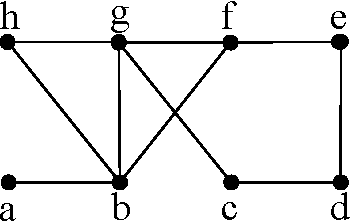
\includegraphics[width=1.0\textwidth,keepaspectratio]{centrsampl/figures/eps/example-betw}
    \caption{Example graph}
  \end{subfigure}
 \hfill
  \begin{subtable}[c]{0.7\textwidth}
  \centering
    \begin{tabular}{ccccccccc}
      \toprule
      Vertex & $\mathrm{a}$ & $\mathrm{b}$ &$\mathrm{c}$ &$\mathrm{d}$ &$\mathrm{e}$ &$\mathrm{f}$ &$\mathrm{g}$ &$\mathrm{h}$ \\
      \midrule
      $\betw(v)$ & 0 & 0.250 & 0.125 & 0.036 & 0.054 & 0.080 & 0.268 & 0 \\
      \bottomrule
    \end{tabular}
    \caption{Betweenness values}
  \end{subtable}
  \caption{Example of betweenness values}
  \label{fig:centrsamplexample-betw}
\end{figure}
\fi

It is easy to see that $\betw(v)\in[0,1]$. \citet{Brandes01} presented an
algorithm to compute the betweenness centrality for all $v\in V$ in time
$O(nm)$ for unweighted graphs and $O(nm + n^2 \log n)$ for weighted graphs. 

\ifproof
We present many variants of betweenness in Sect.~\ref{sec:centrsamplvariants}.
\else
A ``local'' variant of betweenness, called \emph{$k$-bounded-distance
betweenness}\footnote{Bounded-distance betweenness is also known as
$k$-betweenness. We prefer the former denomination to avoid confusion with
$k$-path betweenness.} only considers
the contribution of shortest paths of size up to $k+1$~\citep{BorgattiE06,Brandes08}.
For $k>1$ and any pair of distinct vertices $u,v\in V$, $u\neq V$, let
$\mathcal{S}^{(k)}_{uv}\subseteq\mathcal{S}_{uv}$ be the set of shortest paths
from $u$ to $v$ of size at most $k+1$, with
$\sigma^{(k)}_{uv}=|\mathcal{S}^{(k)}_{uv}|$, and let $\mathbb{S}^{(k)}_G$ be the
union of all the $\mathcal{S}^{(k)}_{uv}$. Let
$\mathcal{T}^{(k)}_v\subseteq\mathcal{T}_v$ be the set of all shortest paths
\emph{of size up to $k$} that $v$ is internal to, for each $v\in V$.

%\begin{definition}[\citep{BorgattiE06,Brandes08}]\label{def:centrsamplkboundbetweenness}
\begin{definition}\label{def:centrsamplkboundbetweenness}
  \citep{BorgattiE06,Brandes08} Given a graph $G=(V,E)$ and an integer $k>1$,
  the \emph{$k$-bounded-distance betweenness centrality of a vertex $v\in V$} is
  defined as
  \[
  %\betw(v)=\sum_{(u,w)\in V\times
  %V}\sum_{p\in\mathcal{S}_{uw}}\frac{\mathds{1}_{\mathcal{T}_v}(p)}{|\mathcal{S}_{uw}|}\enspace.
  %\betw(v)=\sum_{p_{uw}\in\mathbb{S}_G}\frac{\mathds{1}_{\mathcal{T}_v}(p)}{|\mathcal{S}_{uw}|}\enspace.
  \kboundbetw^{(k)}(v)=\frac{1}{n(n-1)}\sum_{p_{uw}\in\mathbb{S}^{(k)}_G}\frac{\mathds{1}_{\mathcal{T}^{(k)}_v}(p)}{\sigma^{(k)}_{uw}}
  %=\frac{1}{n(n-1)}\sum_{p_{uw}\in\mathcal{T}^{(k)}_v}\frac{1}{\left|\mathcal{S}^{(k)}_{uw}\right|}
  \enspace.
  \]
\end{definition}
Other variants of centrality are presented in the extended
version~\citep{RiondatoK13}.
\fi


\section{A range space of shortest paths}\label{sec:centrsamplrangeset}
We now define a range space of the shortest paths of a graph $G=(V,E)$, and present 
a strict upper bound to its VC-dimension. %We show that this upper bound is strict. 
We use the range space and the bound in the analysis of our algorithms for estimating
the betweenness centrality of vertices of $G$.

The range space $\range_G$ is defined on the set $\mathbb{S}_G$ of all shortest
paths between vertices of $G$. It contains, for each vertex $v\in V$, the set
$\mathcal{T}_v$ of shortest paths that $v$ is internal to:
\[
\range_G = \{\mathcal{T}_v ~:~ v\in V\}\enspace.
\]

\begin{lemma}\label{lem:vcdimuppbound}
  %Given a graph $G=(V,E)$ with vertex-diameter $\Delta_G$, the range space
  %$\range_G$ associated to the shortest paths in $G$ has VC-dimension
  $\VC(\range_G)\le\lfloor\log_2(\VD(G)-2)\rfloor+1$.
\end{lemma}

\begin{proof}
%\begin{IEEEproof}
Let $\ell>\lfloor\log_2(\VD(G)-2)\rfloor+1$ and assume for the sake of contradiction
that $\VC(\range_G)=\ell$. From the definition of the VC-dimension there is a set
$Q\subseteq\mathbb{S}_G$ of size $\ell$ that is shattered by $\range_G$. Let $p$ be
an element of $Q$. There are  $2^{\ell-1}$ non-empty subsets of
$Q$ containing the path $p$. Let us label these non-empty subsets of $Q$ containing $p$ as
$S_1,\dotsc,S_{2^{\ell-1}}$, where the labelling is arbitrary.
Given that $Q$ is shattered, for each set $S_i$ there must be a range $R_i$ in
$\range_G$ such that $S_i=Q\cap R_i$. Since all the $S_i$'s are
different from each other, then all the $R_i$'s must be different from each
other. Given that $p$ belongs to each $S_i$, then $p$ must also belong to each
$R_i$, that is, there are $2^{\ell-1}$ distinct ranges in $\range_G$ containing
$p$. But $p$ belongs only to the ranges corresponding to internal vertices of
$p$, i.e., to vertices in $\mathsf{Int}(p)$. This means that the number of ranges
in $\range_G$ that $p$ belongs to is equal to $|p|-2$. But $|p|\le\VD(G)$, by
definition of $\VD(G)$, so $p$
can belong to at most $\VD(G)-2$ ranges from $\range_G$. Given that
$2^{\ell-1}>\VD(G)-2$, we reached a contradiction and there cannot be $2^{\ell-1}$
distinct ranges containing $p$, hence not all the sets $S_i$ can be expressed as
$Q\cap R_i$ for some $R_i\in\range_G$. Then $Q$ cannot be shattered and
$\VC(\range_G)\le\lfloor\log_2(\VD(G)-2)\rfloor+1$.%\qed
\end{proof}
%\end{IEEEproof}

\paragraph{Unique shortest paths}\label{sec:centrsamplrangeunique}
In the restricted case when the graph is undirected and
every pair of distinct vertices has either none or a unique shortest path
between them, the VC-dimension of $\range_G$ reduces %collapses 
to a \emph{constant}. This is a
somewhat surprising result with interesting consequences. From a theoretical
point of view, it suggests that there should be other characteristic
quantities of the graph different from the vertex diameter that control the
VC-dimension of the range space of shortest paths, and these quantities are
constant on graph with unique shortest paths between vertices. From a more
practical point of view, we will see in Sect.~\ref{sec:centrsamplalgo} that this result has an
impact on the sample size needed to approximate %for approximating 
the betweenness centrality of
networks where the unique-shortest-path property is satisfied or even enforced,
like road networks~\citep{GeisbergerSS08}. In particular, the resulting sample
size will be \emph{completely independent} from any characteristic of the
network, and will only be a function of the parameters controlling the desired
approximation guarantees. We are currently investigating whether this result can
be extended to the case of directed graphs.
\ifproof
\else
Due to space constraints, we defer the proof to the extended online version of
the paper~\citep{RiondatoK13}.
\fi

\begin{lemma}\label{lem:vcdimuppboundunique}
  Let $G=(V,E)$ be an undirected graph with $|\mathcal{S}_{uv}|\le1$ for all
  pairs $(u,v)\in V\times V$. Then $\VC(\range_G)\le 3$.
%  Given an undirected
%  graph $G=(V,E)$ such that $|\mathcal{S}_{uv}|\le1$ for all
%  pairs $(u,v)\in V\times V$, the range space $\range_G$ of the
%  shortest paths in $G$ has VC-Dimension $\VC(\range_G)\le3$.
\end{lemma}

\ifproof
\begin{proof}
%\begin{IEEEproof}
  First of all, notice that in this restricted setting, if two different
  shortest paths $p_1$ and $p_2$ meet at a vertex $u$, then they either go on
  together or %at a certain point 
  they separate never to meet again at any other
  vertex $v\neq u$. This is easy to see: if they could separate at $u$ and then
  meet again at some $v$, then there would be two distinct shortest paths
  between $u$ and $v$, which is a contradiction of the hypothesis. Let us denote
  this fact as $\mathsf{F}$.

  Assume now that $\VC(\range_G)>3$, then there must be a set
  $Q=\{p_1,p_2,p_3,p_4\}$ of four shortest paths that can be shattered by
  $\range_G$. Then there is a vertex $w$ such that $\mathcal{T}_w\cap Q=Q$, i.e.,
  all paths in $Q$ go through $w$. Let $x$ be the farthest predecessor of $w$
  along $p_1$ that $p_1$ shares with some other path from $Q$, and let $y$ be
  the farthest successor of $w$ along $p_1$ that $p_1$ shares with some other
  path from $Q$. It is easy to see that if either $x$ or $y$ (or both) do not
  exist, then $Q$ cannot be shattered, as we would incur in a contradiction of
  fact $\mathsf{F}$. 
  
  Let us then assume that both $x$ and $y$ exist.
  Let $Q_x=\mathcal{T}_x\cap Q$ and $Q_y=\mathcal{T}_y\cap Q$.
  Because of fact $\mathsf{F}$, all paths in $Q_x$ must go through the same vertices
  between $x$ and $w$ and all paths in $Q_y$ must go through the same vertices
  between $w$ and $y$. This also means that all paths in $Q_x\cap Q_y$ must go
  through the same vertices between $x$ and $y$. If $Q_x\cup Q_y\neq Q$, let
  $p^*\in Q\setminus(Q_x\cup Q_y)$. Then from the definition of $x$ and $y$ and
  from fact $\mathsf{F}$ we have that there is no vertex $v$ such that
  $\mathcal{T}_v\cap Q=\{p_1,p^*\}$, which implies that $Q$ can not be
  shattered. 
  
  Suppose from now on that $Q_x\cup Q_y=Q$.  If $Q_x\cap Q_y=Q$, then
  all the paths in $Q$ go through the same vertices between $x$ and $y$. From
  this and the definition of $x$ and $y$ we have that there is no vertex $v$
  such that, for example, $\mathcal{T}_v\cap Q=\{p_1,p_2\}$, hence $Q$ cannot be
  shattered. Suppose instead that $Q_x\cap Q_y\neq Q$ and let $S=(Q_x\cap
  Q_y)\setminus\{p_1\}$. If $S\neq\emptyset$ then there is at least a path
  $p'\in S$ which, from the definition of $S$ and fact $\mathsf{F}$, must go
  through all the same vertices as $p_1$ between $x$ and $y$. Moreover, given
  that $Q_x\cap Q_y\neq Q$, there must be a path $p^*\in Q\setminus\{p_1\}$
  different from $p_1$ such that $p^*\notin S$. Then, from the definition of
  $x$, $y$, and $S$, and from the existence of $p'$, there can be no vertex $v$
  such that $\mathcal{T}_v\cap Q=\{p_1,p^*\}$, hence $Q$ cannot be shattered.
  Assume now that $S=\emptyset$ and consider the case $Q_x=\{p_1,p_2,p_3\}$,
  $Q_y=\{p_1,p_4\}$ (all other cases follow by symmetry with this case).
  Consider the set $\{p_1,p_3\}$. From the definition of $x$ and $Q_x$, and from
  fact $\mathsf{F}$ we have that there can not be a vertex $v$ between the end
  point of $p_1$ before $x$ and $w$ such that $\mathcal{T}_v\cap Q=\{p_1,p_3\}$.
  At the same time, from the definition of $y$ and from fact $\mathsf{F}$, we
  have that such a $v$ can not be between $w$ and the end point of $p_1$ after
  $y$. This implies that $Q$ can not be shattered.

  We showed that in all possible cases we reached a contradiction and $Q$,
  which has size $4$, can not be shattered by $\range_G$. Hence $\VC(\range_G)\le
  3$.
%\end{IEEEproof}
\end{proof}
\fi

\ifproof
\else
%\subsection{Variants}\label{sec:centrsamplrangevariants}
\paragraph{Bounded-distance betweenness}
For the case of $k$-bounded-distance betweenness, if we let
$\range_G^{(k)}=\{\mathcal{T}_v^{(k)}~:~ v\in V\}$, it is easy to bound
$\VC(\range_G^{(k)})$ following the same reasoning as in
Lemma~\ref{lem:vcdimuppbound}.
\begin{lemma}\label{lem:vcdimuppboundk}
$\VC(\range_G^{(k)})\le\lfloor\log_2(k-1)\rfloor+1$.
\end{lemma}
\fi

\subsection{Tightness}\label{sec:centrsampltightness}
The bound presented in Lemma~\ref{lem:vcdimuppbound} is strict in the sense that
for each $d\ge 1$ we can build a graph $G_d$ with vertex-diameter
$\VD(G_d)=2^d+1$ and such that the range space $\range_{G_d}$ associated to the set of
shortest paths of $G_d$ has VC-dimension exactly
$d=\lfloor\log_2(\VD(G_d)-2)\rfloor+1$. 
%For the sake of clarity, we will discuss
%only the case of undirected graphs with equal edge weights, but all we say can
%be easily adapted to the general case.

\ifproof
We now introduce a class $\mathcal{G}=(G_d)_{d\ge 1}$ of graphs indexed by $d$.
The graphs in $\mathcal{G}$ are the ones for which we can show the tightness of
the bound to the VC-dimension of the associated range space.
We call the graph $G_d\in\mathcal{G}$ the \emph{$d$\textsuperscript{th} concertina graph}.
Figure~\ref{fig:centrsampltightgraphs} shows $G_1$, $G_2$, $G_3$, and $G_4$. The
generalization to higher values of $d$ is be straightforward.
By construction, $\VD(G_d)=2^d+1$, so that
$\lfloor\log_2(\VD(G_d)-2)\rfloor+1=d$. The $3(2^{d-1})$ vertices of $G_d$ can
be partitioned into three classes, \emph{top}, \emph{bottom}, and \emph{middle},
according to their location in a drawing of the graph similar to those in
Fig.~\ref{fig:centrsampltightgraphs}. $G_d$ has $2^{d-1}-1$ top vertices, $2^{d-1}-1$ bottom vertices, and
$2^{d-1}+2$ middle vertices. For each top vertex $v$, let $\mathsf{f}(v)$ be the
\emph{corresponding bottom vertex}, i.e., the bottom vertex $u$ whose neighbors
are the same middle vertices that are neighbors of $v$. Among the middle
vertices, the two with degree 1 are special and are called the \emph{end
vertices} of $G_d$ and denoted as $v_\ell$ and $v_\mathrm{r}$, where the
labels can be arbitrarily assigned. We now build a set $Q$ of $d$
shortest paths from $v_\ell$ to $v_\mathrm{r}$ and show that it is
shattered by $\range_{G_d}$, therefore proving that $\VC(\range_{G_d})\ge d$.
This fact, together with Lemma~\ref{lem:vcdimuppbound}, allows us to conclude
that $\VC(\range_{G_d})=d$. 
\else
There is a class $\mathcal{G}=(G_d)_{d\ge 1}$ of graphs indexed by d, such that
the graphs in $\mathcal{G}$ are the ones for which we can show the tightness of
the bound to the VC-dimension of the associated range space. We call the graph
$G_d\in\mathcal{G}$ the \emph{$d$-th concertina graph}.
Figure~\ref{fig:centrsampltightgraphs} shows $G_1$, $G_2$, $G_3$, and $G_4$. The
generalization to higher values of $d$ should be straightforward. Each graph
$G_d$ has $3(2^{d-1}$ vertices and vertex-diameter $d$.
\fi
\begin{lemma}\label{lem:vcdimlowbound}
  $\VC(\range_{G_d})=d$.
\end{lemma}
\ifproof
\begin{proof}
%\begin{IEEEproof}
  As we said, the $d$ paths in $Q$  go from $v_\ell$ to $v_\mathrm{r}$.
  From this and the definition of $G_d$ it should be clear that they must go through
  all the middle vertices of $G_d$. Consider now the set
  $S=2^Q\setminus\{Q,\emptyset\}$. We now build a map $\mathsf{r}$
  from the elements of $S$ to the set of top and bottom vertices of $G_d$. We can
  partition $S$ in two sets $A$ and $B$ as follows: %such that $A\cap
  %B=\emptyset$ and $A\cup B=Q$ in the following way: 
  for each unordered pair $(s',s'')$ of
  elements in $S$ such that $s'\cap s''=\emptyset$ and $s'\cup s''=Q$
  we put $s'$ in $A$ and $s''$ in $B$. It is
  easy to see that the size of $A$ ($|A|=2^{d-1}-1$) equals the number of top
  vertices of $G_d$, and analogously for $B$ and the number of bottom vertices.
  The bijection $\mathsf{r}$ will map the
  elements of $A$ to the top vertices of $G_d$ and the elements of $B$ to the
  bottom vertices. For each $s'\in A$, let $\mathsf{c}(s')$ be the unique element $s''$
  of $B$ such that $s'\cap s''=\emptyset$ and $s'\cup s''=Q$ (i.e.,
  $\mathsf{c}(s')=Q\setminus s'$). 
  Let $\mathsf{r}_A$ be an arbitrary one-to-one map from the elements of $A$ to
  the top vertices of $G_d$. Consider now the inverse map $\mathsf{r}^{-1}_A$
  from the top vertices to the elements of $A$. We can create another map
  $\mathsf{r}_B$ from $B$ to the
  bottom vertices of $G_d$ that maps the element
  $\mathsf{c}(\mathsf{r}^{-1}_A(v))$ of $B$ to the bottom vertex $\mathsf{f}(v)$
  corresponding to $v$, for each top vertex $v$. A path $p\in Q$ goes through
  a top vertex $v$ if and only if $p\in\mathsf{r}^{-1}_A(v)$. Analogously, $p$
  goes through a bottom vertex $u$ if and only if $p\in\mathsf{r}^{-1}_B(u)$.
  It is easy to see that, if we combine $\mathsf{r}_A$ and
  $\mathsf{r}_B$, we obtain a map $\mathsf{r}$ from $S$ to the set of
  top and bottom vertices of $G_d$. An example of a possible $\mathsf{r}$ for
  $G_3$ is presented in Fig.~\ref{fig:centrsamplmapexample}.

  \begin{figure}[ht]
    \centering
    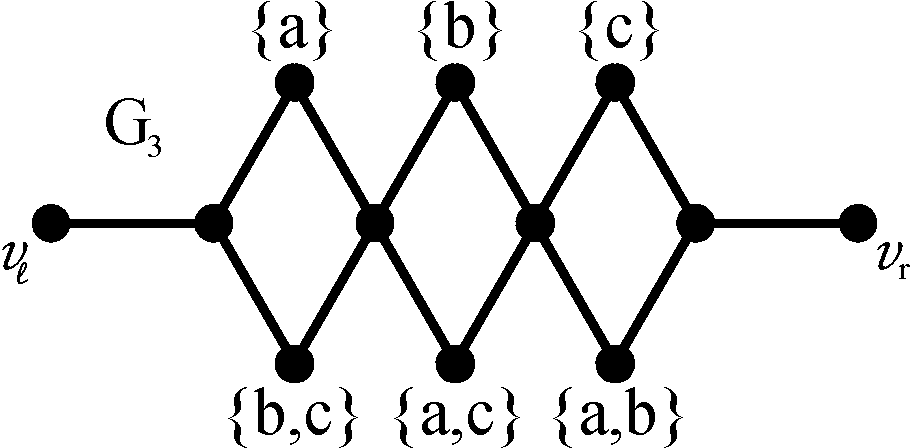
\includegraphics[scale=0.4]{centrsampl/figures/eps/tight-mapexample}
    \caption{An example of the $\mathsf{r}$ map for $G_3$. The set next to
    each top and bottom vertex $u$ is the set $s$ such that $\mathsf{r}(s)=u$.}
    \label{fig:centrsamplmapexample}
  \end{figure}
  
  We now show that for each $s\in S$, $s=Q\cap\mathcal{T}_{\mathsf{r}(s)}$. This
  is easy to see as $\mathsf{r}(s)$ is internal to all paths in $s$, by
  definition of $\mathsf{r}(s)$ and of the paths in $Q$. On the other end, no
  path from $\mathsf{c}(s)$ goes through $\mathsf{r}(s)$ because it goes through
  the corresponding vertex of $\mathsf{r}(s)$ (top if $\mathsf{r}(s)$ is a
  bottom vertex, bottom otherwise). It is also straightforward to see that,
  if we let $v_Q$ be any arbitrary middle vertex different from $v_\ell$
  or $v_\mathrm{r}$, we have $Q=Q\cap\mathcal{T}_{v_Q}$, given that all paths in
  $Q$ go through all the middle vertices. Also, given that $v_\ell$ is not
  internal to any path, we have $\emptyset=Q\cap\mathcal{T}_{v_\ell}$. Then all
  subsets of $Q$ can be expressed as the intersection between $Q$ and a range
  from $\range_{G_d}$, which means that $Q$ can be shattered and therefore
  $\VC(\range_{G_d})\ge d$.

  From Lemma~\ref{lem:vcdimuppbound} we know that $\VC(\range_{G_d})\le d$, so
  it must be $\VC(\range_{G_d})=d$.
%\end{IEEEproof} 
\end{proof}
\else
Due to space constraints, we defer the proof to the extended online version of
the paper~\citep{RiondatoK13}.
\fi

\begin{figure}[th]
  \centering
  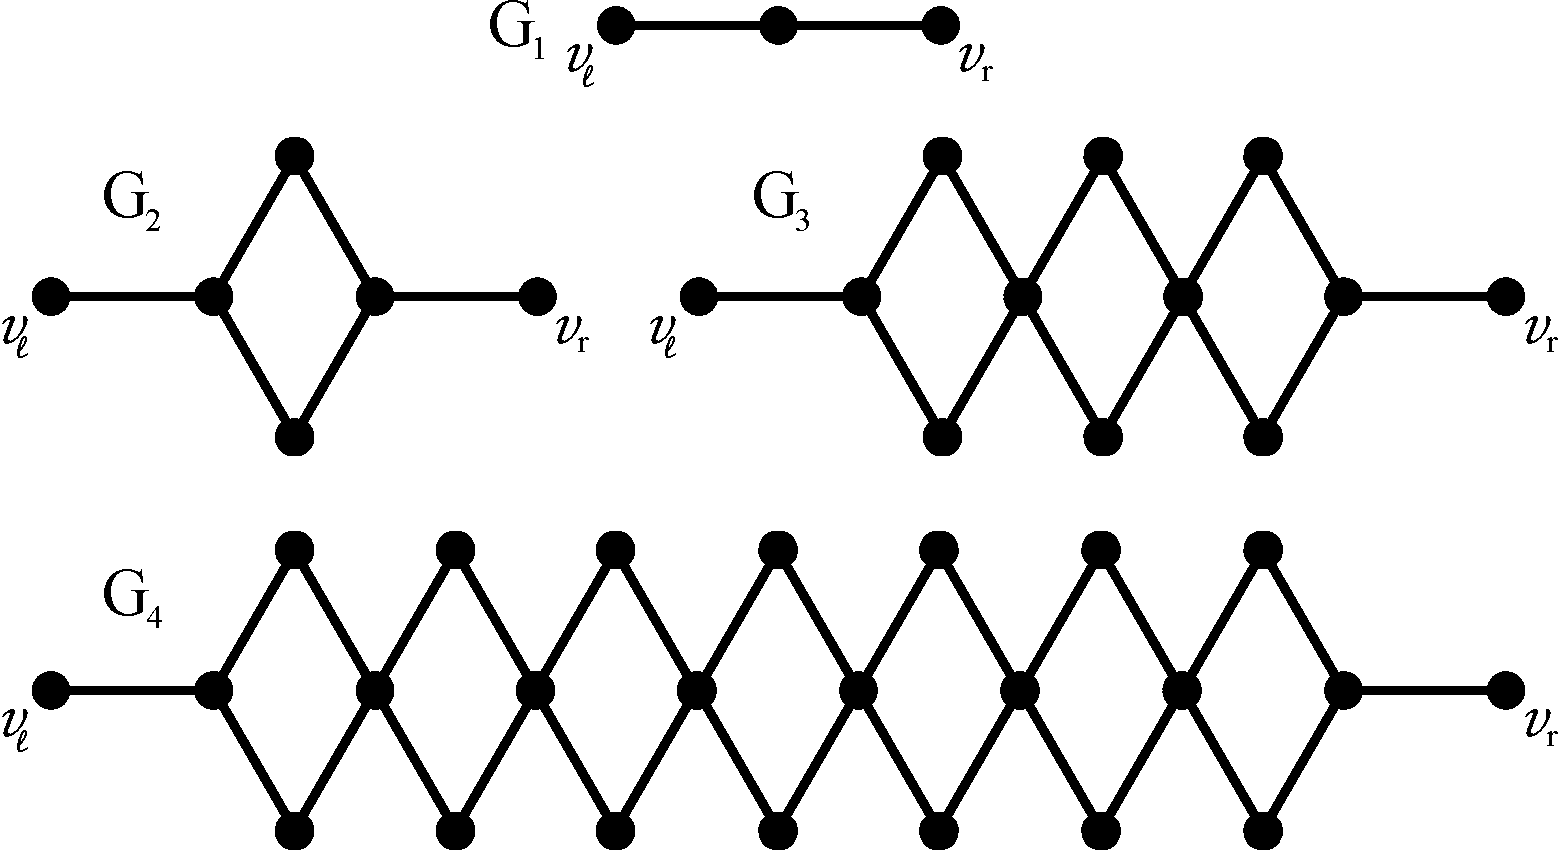
\includegraphics[scale=0.3]{centrsampl/figures/eps/tight}
  \caption{Examples of concertina graphs $G_d$ for $d=1,2,3,4$.}
  \label{fig:centrsampltightgraphs}
\end{figure}

The upper bound presented in Lemma~\ref{lem:vcdimuppboundunique}  for the case
of unique shortest paths is also strict in the same sense.
\ifproof
\else
The proof can be found in the extended online version of the
paper~\citep{RiondatoK13}.
\fi

\begin{lemma}\label{lem:vcdimlowboundunique}
  There is a graph $G=(V,E)$ with $|\mathcal{S}_{uv}|\le1$ for all
  pairs $(u,v)\in V\times V$ such that the range space $\range_G$ associated to the
  shortest paths in $G$ has VC-Dimension exactly $3$.
\end{lemma}

\ifproof
\begin{figure}[ht]
  \centering
  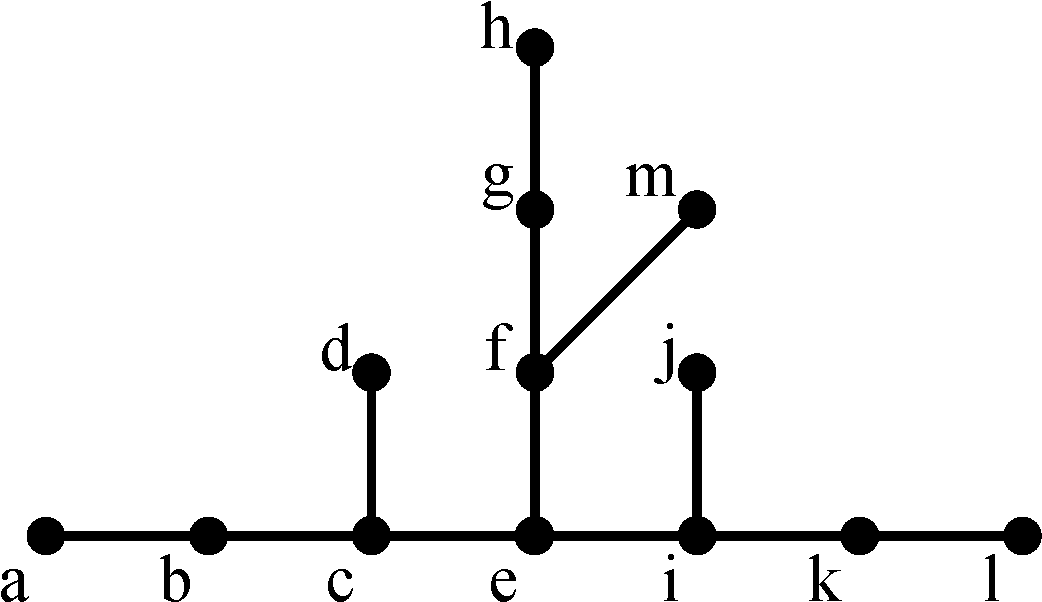
\includegraphics[scale=0.35]{centrsampl/figures/eps/uniqueshortestpathtight}
  \caption{Graph $G$ with $\VC(\range_G)= 3$.}
  \label{fig:centrsampluniquetight}
\end{figure}

\begin{proof}
%\begin{IEEEproof}
  Consider the graph $G$ in Fig.~\ref{fig:centrsampluniquetight}.
  Let $p_1=(a,b,c,e,i,j)$, $p_2=(m,f,e,i,k,l)$, $p_3=(d,c,e,f,g,h)$ be three
  paths. We now show that $Q=\{p_1,p_2,p_3\}$ can be shattered by $\range_G$, which
  implies $\VC(\range_G)\ge 3$. We have $\emptyset=Q\cap\mathcal{T}_a$,
  $\{p_1\}=Q\cap\mathcal{T}_b$, $\{p_2\}=Q\cap\mathcal{T}_k$,
  $\{p_3\}=Q\cap\mathcal{T}_g$, $\{p_1,p_2\}=Q\cap\mathcal{T}_i$,
  $\{p_1,p_3\}=Q\cap\mathcal{T}_c$, $\{p_2,p_3\}=Q\cap\mathcal{T}_f$,
  $\{p_1,p_2,p_3\}=Q\cap\mathcal{T}_e$,  
  Hence all subsets of $Q$ can be expressed as the intersection between $Q$ and
  some range in $\range_G$ which means that $Q$ can be shattered and
  $\VC(\range_G)\ge 3$. Lemma~\ref{lem:vcdimuppboundunique} gives us an upper
  bound $\VC(\range_G)\le3$, so we can conclude that $\VC(\range_G)=3$.
%\end{IEEEproof}
\end{proof}
\fi


\section{Algorithms}\label{sec:centrsamplalgo}
In this section we present our algorithms to compute a set of approximations for the
betweenness centrality of the (top-$K$) vertices in a graph through sampling,
with probabilistic guarantees on the quality of the approximations.

\subsection{Approximation for all the vertices}\label{sec:centrsamplallvertapprox}
The intuition behind the algorithm to approximate the betweenness values of all
vertices is the following. Given a graph $G=(V,E)$
with vertex-diameter $\VD(G)$ and two parameters $\varepsilon,\delta\in(0,1)$
we first compute a sample size $r$ using~\eqref{eq:vceapprox} with
\[d=\lfloor\log_2(\VD(G)-2)\rfloor+1\enspace.\]
The resulting sample size is
\begin{equation}\label{eq:centrsamplsamplesize}
r=\frac{c}{\varepsilon^2}\left(\lfloor\log_2(\VD(G)-2)\rfloor+1+\ln\frac{1}{\delta}\right)\enspace.
\end{equation}
This is sufficient to achieve the desired accuracy
(expressed through $\varepsilon$) with the desired confidence (expressed through
$1-\delta$). The algorithm repeats the following steps $r$ times:
\emph{1.}~it samples a pair $u,v$ of distinct vertices uniformly at random,
\emph{2.}~it
computes the set $\mathcal{S}_{uv}$ of all shortest paths between $u$ and $v$,
\emph{3.}~it selects a path $p$ from $\mathcal{S}_{uv}$ uniformly at random,
\emph{4.}~it increases by $1/r$ the betweenness estimation of each vertex in
$\mathsf{Int}(p)$. Note that if the sampled vertices $u$ and $v$ are not
connected, we can skip steps 3 and 4 because we defined
$\mathcal{S}_{uv}=\{p_\emptyset\}$. Denoting with $S$ the set of the sampled
shortest paths, the \emph{unbiased} estimator $\tilde\betw(w)$ for the betweenness
$\betw(w)$ of a vertex $w$ is the sample average 
\[
\tilde\betw(w) = \frac{1}{r}\sum_{p\in S}
\mathds{1}_{\mathsf{Int}(p)}(w) = \frac{1}{r}\sum_{p\in S}
\mathds{1}_{\mathcal{T}_w}(p)\enspace.
\]

There are two crucial steps in this algorithm: the computation of $\VD(G)$ and
the sampling of a path uniformly at random from $\mathcal{S}_{uv}$. We first
deal with the latter, and then present a linear-time constant-factor approximation algorithm for $\VD(G)$.
%in Sect.~\ref{sec:centrsampldiam}. 
Algorithm~\ref{alg:algorithm} presents the pseudocode of the algorithm,
including the steps to select a random path.  The
\texttt{computeAllShortestPaths(}$u,v$\texttt{)}  on
line~\ref{algline:shortestpaths} is a call to a modified Dijkstra's (or BFS)
algorithm to compute the set $\mathcal{S}_{uv}$, with the same modifications
as~\citep{Brandes01}. The \texttt{getDiameterApprox()} procedure computes an approximation for $\VD(G)$. % (see Sect.~\ref{sec:centrsampldiam} for details).

\paragraph{Unique shortest paths.} 
When, for each pair $(u,v)$ of vertices of $G$, either there is a unique
shortest path from $u$ to $v$ or $v$ is unreachable from $u$, 
%When each pair $(u,v)$ of vertices of $G$ has a unique shortest path connecting them or
%When there is an unique shortest
%path between each pair of vertices of $G$, 
 then one can apply Lemma~\ref{lem:vcdimuppboundunique} and obtain a smaller
sample size
\[
  r= \frac{c}{\varepsilon^2}\left(3+\ln\frac{1}{\delta}\right)
\]
to approximate the betweenness values of all the vertices. 
This is an interesting result: the number of samples needed to compute a good
approximation to all vertices is a \emph{constant} and completely
\emph{independent from $G$}. Intuitively, this means that the algorithm is
extremely fast on graphs with this property. Unique shortest paths are common or
even enforced in road networks by slightly perturbing the edge weights or having
a deterministic tie breaking policy~\citep{GeisbergerSS08}.

\paragraph{Sampling a shortest path.}
Our procedure to select a random shortest path from $\mathcal{S}_{uv}$ is
inspired by the dependencies accumulation procedure used in Brandes' exact
algorithm~\citep{Brandes01}. Let $u$ and $v$ be the vertices sampled by our algorithm
(Step~\ref{algline:samplevertices} of Alg.~\ref{alg:algorithm}). We assume that $u$ and
$v$ are connected otherwise the only possibility is to select the empty path
$p_\emptyset$. Let $y$ be any vertex belonging to at least one shortest path
from $u$ to $v$. Following~\citet{Brandes01}, we can compute $\sigma_{uy}$ and
$\mathcal{S}_{uy}$ while we compute the set $\mathcal{S}_{uv}$ of all the
shortest paths from $u$ to $v$. We can then use this information to select a
shortest path $p$ uniformly at random from $\mathcal{S}_{uv}$ as follows. For each vertex
$w$ let $P_u(w)$ be the subset of neighbors of $w$ that are \emph{predecessors}
of $w$ along the shortest paths from $u$ to $w$. Let $p^*=\{v\}$. Starting from
$v$, we select one of its predecessors $z\in P_u(v)$ using weighted random
sampling: each $z\in P_u(v)$ has probability $\sigma_{uz}/\sum_{w\in
P_u(v)}\sigma_{uw}$ of being sampled. We add $z$ to $p^*$ and then repeat the
procedure for $z$. That is, we select one of $z$'s predecessors from $P_u(z)$
using weighted sampling and add it to $p^*$, and so on until we reach $u$. Note
that we can update the estimation of the betweenness of the internal vertices
along $p^*$ (the only ones for which the estimation is updated) as we compute
$p^*$.

\begin{lemma}\label{lem:samplpath}
  The path $p^*$ built according to the above procedure is selected uniformly at
  random among the paths in $\mathcal{S}_{uv}$.
\end{lemma}

\begin{proof}
  The probability of sampling $p^*=(u,z_1,\dotsc,z_{|p^*|-2},v)$ equals to the
  product of the probabilities of sampling the vertices internal to $p^*$, hence
  \[
  \Pr(p^*)=\frac{\sigma_{uz_{|p^*|-2}}}{\sigma_{uv}}\frac{\sigma_{uz_{|p^*|-3}}}{\sigma_{uz_{|p^*|-2}}}\dotsb
  \frac{1}{\sigma_{uz_2}}=\frac{1}{\sigma_{uv}}
  \]
  where we used \citep[Lemma3]{Brandes01} which tells us that for $w\neq u$,
  \[
  \sigma_{uw}=\sum_{j\in P_u(w)}\sigma_{uj}
  \]
  and the fact that for $z_1$, which is a neighbor of $u$, $\sigma_{uz_1}=1$.
\end{proof}

\begin{algorithm}[ht]
  \SetKwInOut{Input}{Input}
  \SetKwInOut{Output}{Output}
  \SetKwComment{Comment}{//}{}
  \SetKwFunction{VertexDiameter}{getVertexDiameter}
  \SetKwFunction{SamplePair}{sampleUniformVertexPair}
  \SetKwFunction{SampleUniform}{sampleUniformPath}
  \SetKwFunction{PairShortestPaths}{computeAllShortestPaths}
   \DontPrintSemicolon
  \Input{Graph $G=(V,E)$ with $|V|=n$, $\varepsilon,\delta\in(0,1)$}
  \Output{A set of approximations of the betweenness centrality of the vertices
  in $V$}
  \ForEach{$w\in V$}
  {
  $\tilde\betw(v)\leftarrow 0$
  }
  $\VD(G)\leftarrow$\VertexDiameter{G}\label{alg:diamcomp}\; 
  $r\leftarrow (c/\varepsilon^2)(\lfloor\log_2(\VD(G)-2)\rfloor+\ln(1/\delta))$\;
  \For{$i\leftarrow 1$ to $r$}
  {\label{algline:forloop}
  $(u,v)\leftarrow$\SamplePair{$V$}\label{algline:samplevertices}\;
  $\mathcal{S}_{uv}\leftarrow$\PairShortestPaths{$u,v$}\label{algline:shortestpaths}\;
  \If{$\mathcal{S}_{uv}\neq\{p_\emptyset\}$}
  {
  \Comment{Random path sampling and estimation update}
  $j\leftarrow v$\;
  $s\leftarrow v$\;
  $t\leftarrow v$\;
  \While{$t \neq u$} {
  sample $z\in P_s(t)$ with probability $\sigma_{uz}/\sigma_{us}$\;
  \If{$z\neq u$} {
  $\tilde\betw(z) \leftarrow \tilde\betw(z)+1/r$\;
  $s\leftarrow t$\;
  $t\leftarrow z$\;
  }
  }
  }
  } % end For
  \Return{$\{(v,\tilde\betw(v)), v\in V\}$}
  \caption{Computes approximations $\tilde\betw(v)$ of the betweenness
  centrality $\betw(v)$ for all vertices $v\in V$.}
  \label{alg:algorithm}
\end{algorithm}

\paragraph{Approximating the vertex-diameter.}%\label{sec:centrsampldiam}
The algorithm presented in the previous section requires the value of the
vertex-diameter $\VD(G)$ of the graph $G$ (line
\ref{alg:diamcomp} of Alg.~\ref{alg:algorithm}). 
Computing the exact value of $\VD(G)$ could be done by solving the All Pair
Shortest Paths (APSP) problem, and taking the shortest path with the maximum size.
Algorithms for exactly solving APSP problem such as Johnson's which runs in
$O(V^2\log V+VE)$ or Floyd-Warshall's ($\Theta(V^3)$), would defeat our
purposes: once we have all the shortest paths for the computation of
the diameter, we could as well compute the betweenness of all the vertices exactly. 
Given that Thm.~\ref{thm:eapprox} (and Thm.~\ref{thm:eapprox})  only
requires an upper bound to the VC-dimension of the range set, an approximation
of the vertex-diameter would be sufficient for our purposes. Several refined
algorithms for approximating the diameter are
known~\citep{AingwordCIM99,BoitmanisFL06,RodittyW12}, with various running times
and quality of approximations. We briefly present a well-known and simple
approximation algorithm that has the right balance of accuracy and speed
for our purposes.

Let $G=(V,E)$ be an \emph{undirected} graph where \emph{all the edge weights are
equal}.
It is a well-known result that one can obtain a $2$-approximation
$\widetilde\VD(G)$ of the vertex-diameter $\VD(G)$ of $G$ in time $O(V+E)$ in
the following way: 1.~select a vertex $v\in V$ uniformly at random, 2.~compute
the shortest paths from $v$ to all other vertices in $V$, and 3.~finally take
$\widetilde\VD(G)$ to be the sum of the lengths of the two shortest paths with
maximum size (which equals to the two longest shortest paths) from $v$ to two
distinct other nodes $u$ and $w$. The approximation guarantee follows from the next lemma.

\begin{lemma}\label{lem:diam}
  $\VD(G)\le\widetilde\VD(G)\le 2\VD(G)$.
\end{lemma}
\begin{proof}
  Let $v\in V$ be a vertex that we choose uniformly at random from the set $V$.
  Let also $u,w\in V$ be the two vertices such that the sum of the sizes of the
  shortest paths $p_{vu}$ and $p_{vw}$ is maximized among all the shortest paths
  that have $v$ as a source.  We have $\widetilde\VD(G)\le 2\VD(G)$ because
  $|p_{vu}|,|p_{vw}|\le\VD(G)$, so $|p_{vu}|+|p_{vw}|\le 2\VD(G)$. To see
  that $\widetilde\VD(G)\ge\VD(G)$, consider a pair of vertices $x$ and $z$ such
  that the length of a shortest path between $x$ and $z$ is equal to $\VD(G)$.
  Let $p_{xv}$ be a shortest path between $x$ and $v$ and let $p_{vz}$ be a
  shortest path between $v$ and $z$. 
  From the properties of the shortest paths $p_{vu}$, $p_{vw}$ we have
  $|p_{vu}|+|p_{vw}|\geq |p_{vx}|+|p_{vz}|$. Since the graph is undirected
  $|p_{s,t}|=|p_{t,s}|$ for every $s,t\in V$.
  Therefore:
  \[
    \widetilde\VD(G) = |p_{vu}|+|p_{vw}|\geq |p_{vx}|+|p_{vz}| =
    |p_{xv}|+|p_{vz}|\ge\VD(G)\enspace. 
  \]
  For the last inequality we used the fact that since $\VD(G)$ is the size of
  the shortest path from $x$ to $z$, then every other path (in this case
  $p'_{xz}$ which is the merge of $p_{xv}$ and $p_{vz}$) has greater or equal
  length from $p_{x,z}$.
\end{proof}
In case we have multiple connected components in $G$, we compute an upper bound
to the vertex diameter of each component separately by running the above
algorithm on each component, and then taking the maximum. 
The connected components can be computed in $O(n+m)$ by traversing the graph in
a Breadth-First-Search (BFS) fashion starting from a random $v$.
%Let $\tilde\Delta_{G_{1}},\tilde\Delta_{G_{2}}, \ldots , \tilde\Delta_{G_{k}}$
%be the approximations of the diameter for each of the $k$ connected components
%of $G$ as if they were separate graphs.
%The output of the approximation for the graph $G$, is the maximum of the values
%$\tilde\Delta_{G_{1}},\tilde\Delta_{G_{2}}, \ldots , \tilde\Delta_{G_{k}}$.
The time complexity of the approximation algorithm in the case of multiple
connected components is again $O(n+m)$ since the sum of the vertices of
individual components is $n$ and the sum of edges is $m$. 

The use of the above $2$-approximation in the computation of the
sample size from line~\ref{algline:forloop} of Alg.~\ref{alg:algorithm} results
in at most $c/\varepsilon^2$ additional samples than if we
used the exact value $\VD(G)$. The computation of $\widetilde\VD(G)$
does not affect the running time of our algorithm: for the construction of
the first sample we can reuse the shortest paths from the sampled
vertex $v$ that we used to obtain the approximation. Specifically, we can sample
a new vertex $u\neq v$ and then choose with uniform probability one of the
(already computed) shortest paths between $v$ and $u$.

If the graph is directed and/or not all edge weights are equal, the computation
of a good approximation to $\VD(G)$ becomes more problematic. In particular,
notice that there is no relationship between $\VD(G)$ and $\mathsf{diam}(G)$
when $G$ is weighted, as the shortest path with maximum size may not be the
shortest path with maximum weight. In these cases, one can use the size (number
of vertices) of the largest Weakly Connected Component (WCC), as a loose upper
bound to $\VD(G)$. The WCC's can again be computed in $O(n+m)$ using BFS.  This
quantity can be as high as $n$ but for the computation of the sample size we use
its logarithm, mitigating the crudeness of the bound. In this case our sample
size is comparable to that proposed by~\citet{BrandesP07}. %when there is a
%single WCC, as it would depend on $\log n$,
Nevertheless the amount of work done per sample by our algorithm is still much
smaller (see Sect.~\ref{sec:centrsampldiscussion} and~\ref{sec:centrsamplexper} for more
details). In practice, it is possible that the nature of the network suggests a
much better upper bound to the vertex-diameter of the graph, resulting in a
smaller sample size. %than what suggested by the worst case we just presented.  

\paragraph{Analysis.}\label{sec:centrsamplanalysis}
%The algorithm we described and presented in 
Algorithm~\ref{alg:algorithm} offers
probabilistic guarantees on the quality of all approximations of the betweenness
centrality.
\begin{lemma}\label{lem:correctness}
  With probability at least $1-\delta$, all the approximations computed by the
  algorithm are within $\varepsilon$ from their real value:
  \[
  \Pr\left(\exists v\in V \mbox{ s.t. }
  |\betw(v)-\tilde\betw(v)|>\varepsilon\right)<\delta\enspace .
  \]
\end{lemma}

\begin{proof}
%\begin{IEEEproof}
  For each $p_{uv}\in\mathbb{S}_G$ let
  \[
  \pi_G(p_{uv})=\frac{1}{n(n-1)}\frac{1}{\sigma_{uv}}\enspace.
  \]
  It is easy to see that $\pi_G$ is a probability distribution and
  $\pi_G(p_{uv})$ is the probability of sampling the path $p_{uv}$ during an
  execution of the loop on line~\ref{algline:forloop} in
  Alg.~\ref{alg:algorithm}, given the way that the vertices $u$ and $v$ are
  selected and Lemma~\ref{lem:samplpath}.
  
  Consider the range set $\range_G$ and the probability distribution $\prob_G$.
  Let $S$ be the set of paths sampled during the execution of the algorithm.
  For $r$ as in~\eqref{eq:centrsamplsamplesize}, Thm.~\ref{thm:eapprox} tells us that the sample $S$ is a
  $\varepsilon$-approximation to $(\range_G,\prob_G)$ with probability at least
  $1-\delta$. Suppose that this is indeed the case, then from
  Def.~\ref{def:eapprox} and the definition of $\range_G$ we have that
  \[
  \left|\prob_G(\mathcal{T}_v) - \frac{1}{r}\sum_{p\in
  S}\mathds{1}_{\mathcal{T}_v}(p)\right|=\left|\prob_G(\mathcal{T}_v) -
  \tilde\betw(v)\right|\le\varepsilon, \forall v\in
  V\enspace.
  \]
  From the definition of $\prob_G$ we have
  \[
  \prob_G(\mathcal{T}_v)=\frac{1}{n(n-1)}\sum_{p_{uw}\in\mathcal{T}_v}\frac{1}{\sigma_{uw}}=\betw(v),
  \]
  which concludes the proof.
%\end{IEEEproof}
\end{proof}

\ifproof
\paragraph{Time and space complexity.} Clearly the runtime of the algorithm is
dominated by the computation of the shortest path at each step, which takes time
$O(|V|+|M|)$ if the graph is unweighted (BFS algorithm) and time
$O(|E|+|V|\log|V|)$ otherwise (Dijkstra's algorithm with Fibonacci heap).
This time must then be multiplied by $r$ as in~\eqref{eq:centrsamplsamplesize} to obtain
the final time complexity. The space requirements are dominated by the amount of
memory needed to store the graph, so they are either $O(|V|^2)$ if using an
adjacency matrix, or $O(|V|+|E|)$ if using $|V|$ adjacency lists.
\fi

\subsection{High-quality approximation of the top-$K$ betweenness
vertices}\label{sec:centrsampltopk}
%\XXX It would be great to look at the paper by Ezra, ``Small-Size Relative
%$(p,\varepsilon)$-Approximations for Well-Behaved Range Spaces'', 2012,
%available on the arXiv. She presents a smaller bound to the sample size for a
%relative $(p,\varepsilon$-approximation if the range set is ``well-behaved''. We
%should check whether ours is. (Warning: the paper is not exactly an example of
%clarity\ldots)

Very often in practice one is interested only in identifying the vertices with
the highest betweenness centrality, as they are the ``primary actors'' in the
network. We present here an algorithm to compute a very high-quality
approximation of the set $\TOPK(K,G)$ of the top-$K$ betweenness vertices in a graph
$G=(V,E)$. Formally, let $v_1,\dotsc,v_n$ be a labelling of the vertices in $V$
such that $\betw(v_i)\ge\betw(v_j)$ for $1\le i<j\le n$. Then $\TOPK(K,G)$ is
defined as the set of vertices with betweenness at least $\betw(v_K)$:
\[
\TOPK(K,G)=\{(v,\betw(v)), ~:~ v\in V \mbox{ and } \betw(v)\ge\betw(v_K)\}\enspace.
\]
Note that $\TOPK(K,G)$ may contain more than $K$ vertices. 
%This is in line with
%the definition of the set of top-$k$ Frequent Itemsets in the market basket
%analysis setting \XXX add reference.

Our algorithm works in two phases. Each phase is basically a run of the
algorithm for approximating the betweenness of all vertices. %presented in the previous section. 
The two phases differ in the way they compute the number of paths to sample and
the additional operations at the end of each phase. In the first
phase, we compute a lower bound $\ell'$ to $\betw(v_K)$. In the second phase we
use $\ell'$ to compute the number of samples $r$ needed to obtain a relative
$(\ell',\varepsilon)$-approximation to $(\range_G,\pi_G)$. We use $r$ samples to approximate the betweenness of all vertices again, and
return a collection of vertices that is, with high probability, a superset of
$\TOPK(K,G)$.

Let $\widetilde\VD(G)$ be an upper bound to the vertex-diameter of $G$. Given
$\varepsilon,\delta\in(0,1)$, let $\delta',\delta''$ be two positive reals such
that $(1-\delta')(1-\delta'')\ge(1-\delta)$. Let
\[
r'=\frac{c}{\varepsilon^2}\left(\lfloor\log_2(\widetilde\VD(G)-2)\rfloor+1+\log\frac{1}{\delta'}\right)\enspace.
\]
Let $\tilde\betw'_k$ be the $K$-th highest estimated betweenness obtained using
Algorithm~\ref{alg:algorithm} where $r=r'$, and let
%\[
  $\ell'=\tilde\betw_K-\varepsilon$, %.
%\]
%Let
and
\[
r''=\frac{c'}{\varepsilon^2\ell'}\left((\lfloor\log_2(\widetilde\VD(G)-2)\rfloor+1)\log\frac{1}{\ell'}+\log\frac{1}{\delta''}\right)\enspace.
\]
We run Algorithm~\ref{alg:algorithm} with $r=r''$ and let $\tilde\betw''_K$ be
the so-obtained $K$-th highest estimated betweenness. Let
$\ell''=\min\{\tilde\betw''(v) / (1+\varepsilon) ~:~ v\in V \mbox{ s.t. }
\tilde\betw''(v)\ge\tilde\betw''_K\}$. We
return the collection $\widetilde\TOPK(K,G)$ of vertices $v$ such that
$\tilde\betw''(v)*(1+\varepsilon)/(1-\varepsilon)\ge\ell''$:
\[
\widetilde\TOPK(K,G)= \left\{v\in V ~:~
\tilde\betw''(v)\frac{1+\varepsilon}{1-\varepsilon}\ge\ell''\right\}\enspace.
\]
\ifproof
The pseudocode of the algorithm is presented in Algorithm~\ref{alg:topk}.

\begin{algorithm}[ht]
  \SetKwInOut{Input}{Input}
  \SetKwInOut{Output}{Output}
  \SetKwComment{Comment}{//}{}
  \SetKwFunction{VertexDiameter}{getVertexDiameter}
  \SetKwFunction{SamplePair}{sampleUniformVertexPair}
  \SetKwFunction{SampleUniform}{sampleUniformPath}
  \SetKwFunction{PairShortestPaths}{computeAllShortestPaths}
   \DontPrintSemicolon
  %\dontprintsemicolon
  \Input{a graph $G=(V,E)$ with $|V|=n$, a positive integer $K\le n$, real
  values $\varepsilon,\delta\in(0,1)$}
  \Output{a superset of $\TOPK(K,G)$, with high-quality estimation of the
  betweenness for the vertices in the returned set.}
  $\delta',\delta''\leftarrow$ two positive reals such that
  $(1-\delta')(1-\delta'')\ge(1-\delta)$\;
  $\widetilde\VD(G)\leftarrow$ upper bound to $\VD(G)$\;
  \Comment{First phase}
  $r'\leftarrow\frac{c}{\varepsilon^2}\left(\lfloor\log_2(\widetilde\VD(G)-2)\rfloor+1+\log\frac{1}{\delta''}\right)$\;
  $B'=\{(v,\tilde\betw'(v)) ~:~ v\in V\}\leftarrow$ output of Algorithm~\ref{alg:algorithm} with $r=r'$\;
  $\tilde\betw_K'\leftarrow$ $K$-th highest betweenness value from $B'$, ties
  broken arbitrarily\;
  $\ell'\leftarrow\tilde\betw_K'-\varepsilon$\;
  $r''\leftarrow\frac{c'}{\varepsilon^2\ell'}\left((\lfloor\log_2(\widetilde\VD(G)-2)\rfloor+1)\log\frac{1}{\ell'}+\log\frac{1}{\delta''}\right)$\;
  \Comment{Second phase}
  $B''=\{(v,\tilde\betw''(v)) ~:~ v\in V\}\leftarrow$ output of
  Algorithm~\ref{alg:algorithm} with $r=r''$\;
  $\tilde\betw_K''\leftarrow$ $K$-th highest betweenness value from $B''$, ties
  broken arbitrarily\;
  $\ell''\leftarrow\min\{\tilde\betw''(v)/(1+\varepsilon) ~:~ v \mbox{ s.t. }
  \tilde\betw''(v)\ge\tilde\betw_K''\}$\;
  \Return $\{(v,\tilde\betw''(v)) ~:~ v\in V \mbox{ s.t. }
  \tilde\betw''(v)\frac{1+\varepsilon}{1-\varepsilon}\ge\ell''\}$\;
  \caption{High-quality approximation of the top-$K$ betweenness vertices}
  \label{alg:topk}
\end{algorithm}

\paragraph{Analysis.}
The following lemma shows the properties of the collection $\widetilde\TOPK(K,G)$.
\fi

\begin{lemma}
  With probability at least $1-\delta$, 
  \begin{enumerate}
    \item $\TOPK(K,G)\subseteq \widetilde\TOPK(K,G)$, and
    \item for all $v\in\TOPK(K,G)$ we have
      $|\tilde\betw''(v)-\betw(v)|\le\varepsilon\betw(v)$, and
    \item no vertex $u\in\widetilde\TOPK(K,G)\setminus\TOPK(K,G)$ has an estimated
      betweenness greater than $\ell'(1+\varepsilon)$.
  \end{enumerate}
\end{lemma}
\ifproof
\begin{proof}
%\begin{IEEEproof}
  We start by proving 1. From Thm.~\ref{thm:eapprox} we know that, with probability at least
  $1-\delta'$, a sample of size $r'$ is a $\varepsilon$-approximation to
  $(\range_G,\pi_G)$ and from Thm.~\ref{thm:releapprox} we have that with
  probability at least $1-\delta''$ a sample of size $r''$ is a relative
  $(\ell',\varepsilon)$-approximation to $(\range_G,\pi_G)$. Suppose both these
  events occur, which happens with probability at least $1-\delta$. Then it is
  easy to see that $\ell'\le\betw(v_K)$, as there must be at least $K$ vertices
  with exact betweenness greater or equal to $\ell'$.  Consider now $\ell''$.
  Following the same reasoning as for $\ell'$, it should be clear that
  $\ell''\le\betw(v_K)$. The vertices included in $\widetilde\TOPK(K,G)$ are all and
  only those vertices that \emph{may} have exact betweenness at least $\ell''$,
  which implies that all vertices that have exact betweenness at least
  $\betw(v_K)$ are included in $\widetilde\TOPK(K,G)$. 
  Points 2 and 3 in the thesis follow from the properties of the relative
  $(\ell',\varepsilon)$-approximation (Def.~\ref{def:releapprox}).
%\end{IEEEproof}
\end{proof}
\else
We refer the reader interested in the proof to the extended online version of
the paper~\citep{RiondatoK13}.
\fi

The advantage of using our algorithm to approximate the collection of top-$K$
betweenness vertices consists in the very high-quality approximation of the
betweenness values for the returned set of vertices: they are all within a
multiplicative factor $\varepsilon$ from their exact values. By reverse-sorting
them according to the approximated betweenness, one can obtain a ranking that is
very similar to the original exact one. Previous algorithms could not achieve such a
good ranking as they were only able to approximate the betweenness values to
within an additive error $\varepsilon$. The cost of computing the high quality
approximation for the top-$K$ vertices is the cost of an additional run of our
algorithm to compute good approximations for all the vertices.

\subsection{Discussion}\label{sec:centrsampldiscussion}
\citet{JacobKLPT05} and independently~\citet{BrandesP07} present a
sampling-based algorithm to approximate the betweenness centrality of all the
vertices of the graph. The algorithm (which we call \textsf{BP}) creates a
sample $S=\{v_1,\dotsc,v_r\}$ of $r$ vertices drawn uniformly at random and
computes all the shortest paths between each $v_i$ to all other vertices in the
graph. Their estimation $\tilde\betw_\mathsf{BP}(u)$ for $\betw(u)$ is
\[ 
\tilde\betw_\mathsf{BP}(u)= \frac{1}{(n-1)r}\sum_{v_i\in S}\sum_{\substack{w\neq
v_i\\w\neq
u}}\sum_{p\in\mathcal{S}_{v_iw}}\frac{\mathds{1}_{\mathsf{Int}(p)}(u)}{|\mathcal{S}_{v_iw}|}\enspace.
\]
As it was for Algorithm~\ref{alg:algorithm}, the key ingredient to ensure a correct
approximation for the betweenness centrality is the computation of the sample
size $r$. Inspired by the work of~\citet{EppsteinW04}, \citet{BrandesP07} 
%rely
%on the following classical result by~\citet{Hoeffding63} for their computation
%of $r$.
%\begin{theorem}[\citep{Hoeffding63}]
%  Let $X_1,X_2,\dotsc,X_r$ be a sequence of independent random variables
%  such that $a_i\leq X_i\leq b_i$. Then for any $\xi > 0$
%  \begin{align}\label{eq:centrsamplhoeffding}
%    \begin{split}
%      \Pr&\left(\left|\frac{|\sum_{i=1}^rX_i|}{r}-\mathbf{E}\left[\frac{|\sum_{i=1}^rX_i|}{r}\right]\right|\geq
%    \xi\right)\le \\
%      &\leq 2e^{-2r^2\xi^2/\sum_{i=1}^{r}(b_{i}-a_{i})^2}\enspace.
%    \end{split}
%  \end{align}
%\end{theorem}
%
%\citet{BrandesP07} use this result to compute a sample size $r$ sufficient to ensure that, for
%a fixed vertex $u$,
%\[ 
%\Pr\left(|\betw(u)-\tilde\betw'(u)|>\varepsilon\right)<\frac{\delta}{n}\enspace.
%\]
%In their setting $\xi=\varepsilon$ and there is a variable $X_i$ for
%each vertex $v_i$ in the sample:
%\[ 
%X_i=\frac{1}{n-1}\sum_{w\neq v_i,w\neq
%u}\sum_{p\in\mathcal{S}_{v_iw}}\frac{\mathds{1}_{\mathsf{Int}(p)}(u)}{|\mathcal{S}_{v_iw}|}\enspace
%.
%\]
%It is easy to see that $0\le X_i\le 1$. Moreover,
%\[
%  \mathbf{E}\left[\frac{|\sum_{i=1}^r X_i}{r}\right] = \betw(u)\enspace.
%\]
%%\begin{align*}
%%\mathbf{E}\left[\frac{|X_1+\dotsb+X_r|}{r}\right] &=
%%\frac{1}{r(n-1)}\mathbf{E}\left[\sum_{v_i\in S}\sum_{w\neq v_i,w\neq
%%u}\sum_{p\in\mathcal{S}_{v_iw}}\frac{\mathds{1}_{\mathsf{Int}(p)}(u)}{|\mathcal{S}_{v_iw}|}\right]
%%=\frac{1}{r(n-1)}\sum_{v\in V}\mathbf{E}\left[Y_v\sum_{w\neq v,w\neq
%%u}\sum_{p\in\mathcal{S}_{vw}}\frac{\mathds{1}_{\mathsf{Int}(p)}(u)}{|\mathcal{S}_{vw}|}\right] =
%%\\
%%&=\frac{1}{r(n-1)}\sum_{v\in V}\mathbf{E}[Y_v]\sum_{w\neq v,w\neq
%%u}\sum_{p\in\mathcal{S}_{vw}}\frac{\mathds{1}_{\mathsf{Int}(p)}(u)}{|\mathcal{S}_{vw}|}
%%=\frac{1}{r(n-1)}\sum_{v\in V}\frac{r}{n}\sum_{w\neq v,w\neq
%%u}\sum_{p\in\mathcal{S}_{vw}}\frac{\mathds{1}_{\mathsf{Int}(p)}(u)}{|\mathcal{S}_{vw}|}
%%= \betw(u),
%%\end{align*}
%%where $Y_v$ is a Bernoulli random variable taking value 1 if $v\in S$, and 0
%%otherwise, so $\mathbf{E}[Y_v]=\Pr(Y_v=1)=r/n$.
%Plugging these values in~\eqref{eq:centrsamplhoeffding}, we have
%\[
%\Pr\left(|\betw(u)-\tilde\betw'(u)|>\varepsilon\right)\leq
%2e^{-2r\epsilon^2}\enspace.
%\]
%We want this probability to be at most $\delta/n$, so we need a sample of size
%They
prove that, to obtain good (within $\varepsilon$) estimations for the
betweenness of all vertices with probability at least $1-\delta$, it must be
\[
r\geq \frac{1}{2\varepsilon^2}\left(\ln n + \ln 2 +\ln\frac{1}{\delta}\right)\enspace.
\]
%An application of the union bound over the $n$ vertices ensures a uniform
%(simultaneous) guarantee on the quality of
%all the estimation, with probability at least $1-\delta$.
From this expression it should be clear that this sample size is usually much
larger than ours, as in practice $\VD(G)\ll n$. For the same reason, this
algorithm would not scale well as the network size increases (see also
Sect.~\ref{sec:centrsamplexper}).

Another interesting aspect in which our algorithm and \textsf{BP} differ is the
\emph{amount of work done per sample}. Our algorithm computes a single set
$\mathcal{S}_{uv}$ for the sampled pair of vertices $(u,v)$: it performs a run
of Dijkstra's algorithm (or of BFS) from $u$, stopping when $v$ is reached.
\textsf{BP} instead computes all the sets $\mathcal{S}_{uw}$ from the sampled
vertices $u$ to all other vertices, again with a single run of Dijkstra or BFS,
but without the ``early-stopping condition'' that we have when we reach $v$.
Although in the worst case the two computations have the same time
complexity\footnote{It is a well-known open problem whether there is an
algorithm to perform a single $s,t$-shortest path computation between a pair of
vertices with smaller worst-case time complexity than the Single Source Shortest
Path computation.}, in practice we perform many fewer operations, as we can
expect $v$ not to always be very far from $u$ and therefore we can terminate
early. This fact has a huge impact on the running time. Our algorithm also
touches \emph{many fewer} edges than \textsf{BP}. The latter can touch all the
edges in the graph \emph{at every sample}, while our computation exhibits a much
higher \emph{locality}, exploring only a neighborhood of $u$ until $v$ is
reached. The results of our experimental evaluation presented in
Sect.~\ref{sec:centrsamplexper} highlights this and other advantages of our method over
the one from~\citep{JacobKLPT05,BrandesP07}. 
It would be interesting to explore the %In the future, we plan to
%investigate 
the possibility of using \emph{bidirectional A$^*$
search}~\citep{Pohl69,KaindlK97} to further speed up the computation for each
sample of our algorithms.

The analysis of Algorithm 1 allow us to obtain a tighter analysis for the
algorithm by~\citet{BrandesP07} and~\citet{JacobKLPT05}.

\begin{lemma}\label{lem:variance}
  Fix $r>0$ and let $w\in V$. Let $\tilde\betw_\mathsf{BP}(w)$ be the estimation
  of the betweenness $\betw(w)$ computed by \textsf{BP} using $r$ samples, and
  let $\tilde\betw(w)$ be the estimation computed by
  Algorithm~\ref{alg:algorithm} using $r$ samples. The estimator
  $\tilde\betw_\mathsf{BP}(w)$ is \emph{uniformly better} than the estimator
  $\tilde\betw(w)$. I.e., for any value of $\betw(w)$ and $r$, we have
  \[
  \var[\tilde\betw_\mathsf{BP}(w)]\le\var[\tilde\betw(w)]\enspace.
  \]
\end{lemma}

\begin{proof}
  Consider the quantity
  \[
  \var[\tilde\betw(w)]-\var[\tilde\betw_\mathsf{BP}(w)]\enspace.\]
  We will show that the above quantity is greater than or equal to 0, proving
  the thesis.
  Since
  $\expectation[\tilde\betw(w)]=\expectation[\tilde\betw_\mathsf{BF}(w)]=\betw(w)$
  and using the definition of variance, we only need to show 
  \begin{equation}\label{eq:centrsamplinequal}
    \expectation[(\tilde\betw(w))^2]-\expectation[(\tilde\betw_\mathsf{BF}(w))^2]\ge
    0\enspace.
  \end{equation}

  Let start from computing $\expectation[(\tilde\betw_\mathsf{BF}(w))^2]$. For every
  vertex $v$, we define $\alpha_v$ as
  \[
  \alpha_v=\frac{1}{n-1}\sum_{\substack{u\in V
  \\u\neq
  v}}\sum_{p\in\mathcal{S}_{vu}}\frac{\mathds{1}_{\mathsf{Int}(p)}(w)}{\sigma_{vu}}\enspace.
  \]
  Note that 
  \begin{equation}\label{eq:centrsamplbetwalpha}
    \betw(w)=\frac{1}{n}\sum_{v\in V}\alpha(v)\enspace.
  \end{equation}
  Consider, for $1\le i \le r$, the contribution $X_i$ to $\tilde\betw_\mathsf{BP}(w)$
  of the paths computed from the $i$\textsuperscript{th} sampled vertex. $X_i$
  is a random variable that takes value $\alpha_v$ with probability $1/n$, for
  all $v\in V$. We have
  \begin{equation}\label{eq:centrsamplxiexpvar}
    \expectation[X_i]=\sum_{v\in V}\frac{1}{n}\alpha_v=\betw(w) \mbox{ and }
    \expectation[X_i^2]=\frac{1}{n}\sum_{v\in V}\alpha_v^2, \forall 1\le i\le r\enspace.
  \end{equation}
  Clearly
  \[
  \tilde\betw_\mathsf{BP}(w)=\frac{1}{r}\sum_{i=1}^r X_i\enspace.
  \]
  The variables $X_i$'s are independent and identically distributed so
  \begin{align}\label{eq:centrsamplexpxisquared}
    \expectation[(\tilde\betw_\mathsf{BP}(w))^2]&=\frac{1}{r^2}\expectation\left[\left(\sum_{i=1}^rX_i\right)^2\right]=\frac{1}{r^2}\sum_{i=1}^r\left(\expectation[X_i^2]+\sum_{j=i+1}^r(\expectation[X_i]\expectation[X_j])\right)
    \nonumber\\
    &=\frac{1}{r}\frac{1}{n}\sum_{v\in V}\alpha_v^2+\frac{r-1}{r}(\betw(w))^2,
\end{align}
where we used~\eqref{eq:centrsamplxiexpvar}.

We now compute $\expectation[(\tilde\betw(w))^2]$. 
Consider the contribution $Y_i$ to $\tilde\betw(w)$ of the
$i$\textsuperscript{th} sampled path by Algorithm 1, for $1\le i\le r$. $Y_i$ is a random variable that takes value
$\mathds{1}_{\mathsf{Int}(p)}(w)$ with probability $\pi(p)$, for every shortest
path $p\in\mathbb{S}_G$. We have
\begin{equation}\label{eq:centrsamplyiexpvar}
  \expectation[Y_i]=\expectation[Y_i^2]=\betw(w), \forall 1\le i \le r\enspace.
\end{equation}
By definition, 
\[
\tilde\betw(w)=\frac{1}{r}\sum_{i=1}^rY_i\enspace.
\]
The random variables $Y_i$ are independent and identically distributed so
\begin{align}\label{eq:centrsamplexpyisquared}
  \expectation[(\tilde\betw(w))^2]&=\frac{1}{r^2}\expectation\left[\left(\sum_{i=1}^r
  Y_i\right)^2\right]=\frac{1}{r^2}\sum_{i=1}^r\left(\expectation[Y_i^2]+\sum_{j=i+1}^r\expectation[Y_i]\expectation[Y_j]\right)\nonumber\\
  &=\frac{1}{r}\betw(w)+\frac{r-1}{r}(\betw(w))^2,
\end{align}
where we used~\eqref{eq:centrsamplyiexpvar}.

We can now rewrite the left side of~\eqref{eq:centrsamplinequal} using
~\eqref{eq:centrsamplbetwalpha},~\eqref{eq:centrsamplexpxisquared},~and~\eqref{eq:centrsamplexpyisquared}:
\begin{align*}
  \expectation[(\tilde\betw(w))^2]-\expectation[(\tilde\betw_\mathsf{BF}(w))^2] &=
  \frac{1}{r}\betw(w)+\frac{r-1}{r}(\betw(w))^2 - \frac{1}{r}\frac{1}{n}\sum_{v\in
    V}\alpha_v^2
   -\frac{r-1}{r}(\betw(w))^2 \\
   &= \frac{1}{r}\frac{1}{n}\sum_{v\in V}(\alpha_v - \alpha_v^2)\enspace. 
\end{align*}
Since $\alpha_v\in[0,1]$, we have $\alpha_v-\alpha_v^2\ge 0$ for all $v$, and our proof
is complete.
\end{proof}

The following lemma is an easy consequence of the above.

\begin{lemma}\label{lem:MSE}
  \textsf{BP} has lower expected Mean Squared Error than Algorithm~1:
  \[
  \expectation[\mse_\mathsf{BP}]\le \expectation[\mse]\enspace.
  \]
\end{lemma}

\begin{proof}
  We have
  \[ 
  \expectation[\mse_\mathsf{BP}] = \expectation\left[\frac{1}{n}\sum_{v\in
  V}\left(\tilde\betw_\mathsf{BP}(w)-\betw(v)\right)^2\right]=\frac{1}{n}\sum_{v\in
  V}\expectation\left[\left(\tilde\betw_\mathsf{BP}(w)-\betw(v)\right)^2\right]=\frac{1}{n}\sum_{v\in
  V}\var[\tilde\betw_\mathsf{BP}(w)],
  \]
  where we used the linearity of expectation and the fact that the estimator
  $\tilde\betw_\mathsf{BP}(w)$ is unbiased for $\betw(w)$ ($\expectation[\tilde\betw_\mathsf{BP}(w)]=\betw(w)]$).
  Analogously for Algorithm~1:
  \[
  \expectation[\mse] = \frac{1}{n}\sum_{v\in V}\var[\tilde\betw(w)]\enspace.
  \]
  Hence
  \[
  \expectation[\mse]-\expectation[\mse_\mathsf{BP}]=\frac{1}{n}\sum_{v\in
  V}\left(\var[\tilde\betw(w)]-\var[\tilde\betw_\mathsf{BP}(w)]\right),
  \]
  and from Lemma~\ref{lem:variance} we have that each addend of the sum is
  non-negative and so is the above expression, concluding our proof.
\end{proof}

%\begin{lemma}
%  Let $G=(V,E)$ be a graph, and $\varepsilon,\delta\in(0,1)$. Let
%  \[
%  r =
%  \frac{c}{\varepsilon^2}\left(\lfloor\log_2(\mathsf{VD}(G)-2\rfloor+1+\ln\frac{1}{\delta}\right)\enspace.
%  \]
%  and let $S$ be a set of vertices of $G$ sampled uniformly at random with
%  replacement from $V$. Let $\tilde\betw_{\mathsf{BP}}(w)$ be the estimated
%  value for $\betw(w)$ computed by \textsf{BP} using $S$. Then
%  \[
%  \Pr(\exists w\in V \mbox{ s.t. }
%  |\tilde\betw_{\mathsf{BP}}(w)-\betw(w)|>\varepsilon)<\delta\enspace.
%  \]
%  %If Algorithm 1 computes an $(\varepsilon,\delta)$-approximation with $r$
%  %samples, then the algorithm by~\citet{BrandesP07} does the same with the same
%  %number of samples.
%\end{lemma}
%
%\begin{proof}
%  Consider a simple coupling of the executions of Algorithm 1 and \textsf{BP}
%  for $r$ samples: when Algorithm 1 samples a shortest path from a vertex $v$ to a vertex $u$,
%  \textsf{BP} samples the vertex $v$. 
%
%Consider an execution of the algorithms and let $X_v$ be the number of times
%that vertex $v$ is the starting point of a sampled path. 
%
%The estimation for the betweenness of vertex $w$ computed by \textsf{BP} is
%\[
%\tilde\betw_{\mathsf{BP}}(w)=\frac{1}{r}\sum_{v\in V}
%X_v\underbrace{\left(\frac{1}{n-1}\sum_{\substack{u\in V \\u\neq
%v}}\sum_{p\in\mathcal{S}_{vu}}\frac{\mathds{1}_{\mathsf{Int}(p)}(w)}{|\mathcal{S}_{vu}|}\right)}_{Y_v(w)}\enspace.
%\]
%The estimation for the betweenness of vertex $w$ computed by Algorithm 1
%is
%\[
%\tilde\betw_{\mathrm{A1}}(w)=\frac{1}{r}Z_w,
%\]
%where $Z_w$ is the number of times that a path containing the vertex $w$ gets
%sampled. Now, for each $v$ and for $1\le i\le X_v$, let $p_v^{(i)}$ be the path
%sampled the $i$\textsuperscript{th} time that the sampled path had $v$ as
%starting vertex, and let $A_v^{(i)}(w)=1$ if $w\in\mathsf{Int}(p_v^{(i)}$, and
%$A_v^{(i)}(w)=0$ otherwise. Then it is clear that 
%\[
%\tilde\betw_{\mathrm{A1}}(w)=\frac{1}{r}\sum_{v\in V}
%X_v\frac{\sum_{i=1}^{X_v}A^{(i)}_v(w)}{X_v}\enspace.
%\]
%We claim that
%\[
%\mathbb{E}\left[\left.\frac{\sum_{i=1}^{X_v}A^{(i)}_v(w)}{X_v}\right|X_v\right]=Y_v(w),\]
%where the expectation is taken over the choice of the paths, which are sampled
%according to the distribution $\pi$.
%To see this, consider $\mathbb{E}[A_v^{(i)}(w) ~|~ X_v]$. It
%is clear that $A^{(i)}(w)$ and $X_v$ are independent, for $1\le i\le X_v$. From
%this and the definition of expectation we have 
%\[
%\mathbb{E}\left[\left.A_v^{(i)}(w)\right|X_v\right] =
%\mathbb{E}\left[A_v^{(i)}(w)\right]=\frac{1}{n-1}\sum_{\substack{u\in V
%\\u\neq
%v}}\sum_{p\in\mathcal{S}_{vu}}\frac{\mathds{1}_{\mathsf{Int}(p)}(w)}{|\mathcal{S}_{vu}|}
%=Y_v(w)\enspace.
%\]
%This expression does not depend on $i$.
%
%The claim then follows easily from the linearity of expectation:
%\[
%\mathbb{E}\left[\left.\frac{\sum_{i=1}^{X_v}A^{(i)}_v(w)}{X_v}\right|X_v\right] =
%\sum_{i=1}^{X_v}\mathbb{E}\left[\left.\frac{A^{(i)}_v(w)}{X_v}\right|X_v\right]=\sum_{i=1}^{X_v}\frac{1}{X_v}\mathbb{E}\left[A_v^{(i)}(w)\right]=\mathbb{E}\left[A_v^{(1)}(w)\right]=Y_v(w)\enspace.
%\]
%Recall from Lemma~\ref{lem:variance} that the estimator
%$\tilde\betw_{\mathsf{BP}}(w)$ has lower variance than the estimator
%$\tilde\betw(w)$, for all vertices $w$. 
%
%\XXX: The following is not actually true \MR. Since both estimators have
%the same expectation $\betw(w)$, this means that for any $a\in[0,1]$ we have
%\[
%\Pr\left(|\tilde\betw_{\mathsf{BP}}(w)-\betw(w)|>a\right)\le\Pr(\left(|\tilde\betw(w)-\betw(w)|>a\right)\enspace.
%\]
%
%This means that for every collection of $r$ samples for which Algorithm 1 computes estimates
%$\tilde\betw(w)$ such that
%\begin{equation}\label{eq:centrsampledapprox}
%|\tilde\betw(w)-\betw(w)|\le\varepsilon, \forall w\in W,
%\end{equation}
%so would \textsf{BP} using the $r$ samples according to the coupling. For
%Algorithm $1$ the event in~\eqref{eq:centrsampledapprox} occurs with probability at least
%$1-\delta$ over the choice of samples, and so would be for \textsf{BP},
%concluding our proof.
%\end{proof}
%

The estimator $\tilde\betw_{\mathsf{BP}}(w)$ has lower variance and MSE than
$\tilde\betw(w)$, which means that it can give better estimations of the
betweenness values in practice using the same number of samples. Before always
opting for \textsf{BP} (or for the algorithm by~\citet{GeisbergerSS08}, whose
estimators have even lower variance than those of \textsf{BP}) with a number of
samples equal to the one in~\eqref{eq:centrsamplsamplesize}, one should
nevertheless take into account two facts. Firstly, we do not currently have a
proof that \textsf{BP} (or the algorithm from~\citep{GeisbergerSS08}) can
compute, with a number of samples as in~\eqref{eq:centrsamplsamplesize},
a good (within $\pm\varepsilon$) approximation of the betweenness of all
vertices with probability at least $1-\delta$. We conjecture this fact could be
proven using pseudodimension~\citep[Chap.~11]{AnthonyB99}. %
%\footnote{We conjecture that this is true and are currently working on a
%proof.}
Secondly we already argued that per sample, the computation of
$\tilde\betw_{\mathsf{BP}}(w)$ requires more time than the one for
$\tilde\betw_{\mathrm{A1}}(w)$. The difference would be even larger if
Algorithm~\ref{alg:algorithm} can be adapted to use bidirectional
search~\citep{KaindlK97,Pohl69}. 

We can conclude this discussion stating that Algorithm~\ref{alg:algorithm},
\textsf{BP}, and the algorithm by~\citet{GeisbergerSS08} share the same design
principles, but choose different trade-offs between accuracy and speed.  


\ifproof
%\section{Edge Betweenness and Variants of Vertex Betweenness}\label{sec:centrsamplvariants}
\section{Variants of betweenness centrality}\label{sec:centrsamplvariants}
In this section we discuss how to extends our results to some variants of
betweenness centrality.

\subsection{$k$-bounded-distance betweenness}
A ``local'' variant of betweenness, called \emph{$k$-bounded-distance
betweenness}\footnote{Bounded-distance betweenness is also known as
$k$-betweenness. We prefer the former denomination to avoid confusion with
$k$-path betweenness from~\citep{KourtellisASIT12}.} only considers
the contribution of shortest paths of size up to $k+1$~\citep{BorgattiE06,Brandes08}.
For $k>1$ and any pair of distinct vertices $u,v\in V$, $u\neq V$, let
$\mathcal{S}^{(k)}_{uv}\subseteq\mathcal{S}_{uv}$ be the set of shortest paths
from $u$ to $v$ of size at most $k+1$, with
$\sigma^{(k)}_{uv}=|\mathcal{S}^{(k)}_{uv}|$, and let $\mathbb{S}^{(k)}_G$ be the
union of all the $\mathcal{S}^{(k)}_{uv}$. Let
$\mathcal{T}^{(k)}_v\subseteq\mathcal{T}_v$ be the set of all shortest paths
\emph{of size up to $k$} that $v$ is internal to, for each $v\in V$.

%\begin{definition}[\citep{BorgattiE06,Brandes08}]\label{def:centrsamplkboundbetweenness}
\begin{definition}\label{def:centrsamplkboundbetweenness}
  \citep{BorgattiE06,Brandes08} Given a graph $G=(V,E)$ and an integer $k>1$,
  the \emph{$k$-bounded-distance betweenness centrality of a vertex $v\in V$} is
  defined as
  \[
  %\betw(v)=\sum_{(u,w)\in V\times
  %V}\sum_{p\in\mathcal{S}_{uw}}\frac{\mathds{1}_{\mathcal{T}_v}(p)}{|\mathcal{S}_{uw}|}\enspace.
  %\betw(v)=\sum_{p_{uw}\in\mathbb{S}_G}\frac{\mathds{1}_{\mathcal{T}_v}(p)}{|\mathcal{S}_{uw}|}\enspace.
  \kboundbetw^{(k)}(v)=\frac{1}{n(n-1)}\sum_{p_{uw}\in\mathbb{S}^{(k)}_G}\frac{\mathds{1}_{\mathcal{T}^{(k)}_v}(p)}{\sigma^{(k)}_{uw}}
  %=\frac{1}{n(n-1)}\sum_{p_{uw}\in\mathcal{T}^{(k)}_v}\frac{1}{\left|\mathcal{S}^{(k)}_{uw}\right|}
  \enspace.
  \]
\end{definition}

For the case of $k$-bounded-distance betweenness, if we let
$\range_G^{(k)}=\{\mathcal{T}_v^{(k)}~:~ v\in V\}$, it is easy to bound
$\VC(\range_G^{(k)})$ following the same reasoning as in
Lemma~\ref{lem:vcdimuppbound}.
\begin{lemma}\label{lem:vcdimuppboundk}
$\VC(\range_G^{(k)})\le\lfloor\log_2(k-1)\rfloor+1$.
\end{lemma}

Given this result, the sample size on line~\ref{algline:forloop}
of Alg.~\ref{alg:algorithm} can be reduced to 
\[ 
  r= \frac{c}{\varepsilon^2}\left(\lfloor\log_2(k-1)\rfloor + 1 +\ln\frac{1}{\delta}\right)
\]
and the computation of the shortest paths on line~\ref{algline:shortestpaths}
can be stopped after we reached the vertices that are $k$ ``hops'' far from $u$.

\subsection{$\alpha$-weighted betweenness}
\citet{OpsahlAS10} defined a parametric variant of betweenness centrality for
weighted networks that can be seen as a generalization of the classical 
definition. The goal behind this new definition is to give the analyst the
possibility of ``penalizing'' shortest paths with many vertices, given the
intuition that there is a cost to be paid to have a message go through a vertex.
The core of the new definition is a different weight function of a path
$p_{uv}=(w_1=u,w_2,\dotsc,w_{|p_{uv}|}=v)$ between two vertices $(u,v)$,
parametrized by a real parameter $\alpha\ge 0$:
\begin{equation}\label{eq:centrsamplgeneralizeddistance}
d_{\alpha,uv}=\sum_{i=1}^{|p_{uv}|-1}(\mathsf{w}((w_i,w_{i+1})))^\alpha\enspace. 
\end{equation}
Clearly for $\alpha=0$, the weights are considered all equal to $1$, and for
$\alpha=1$, the definition falls back to $d_{uv}$. For $0<\alpha<1$, paths with
fewer vertices and higher weights are favored over longer paths with lighter
edges\citep{OpsahlAS10}. The definition of shortest path distance, shortest
path, and of betweenness centrality follow as before
from~\eqref{eq:centrsamplgeneralizeddistance}. Dijkstra's shortest paths algorithm can be
adapted to compute shortest paths according to the distance function
in~\eqref{eq:centrsamplgeneralizeddistance}. To avoid confusion, we call the betweenness
centrality computed using the shortest paths according to the distance function
in~\eqref{eq:centrsamplgeneralizeddistance}, the \emph{$\alpha$-weighted betweenness} and
denote it with $\betw_\alpha(w)$. 

For $\alpha$-weighted betweenness we have that the VC-dimension of the range set
defined on the shortest paths according to the distance
from~\eqref{eq:centrsamplgeneralizeddistance} is still bounded by
$\lfloor\log_2(\VD(G)-1)\rfloor+1$. Clearly, the vertex-diameter $\VD(G)$ is now
defined as the maximum number of vertices in a shortest path according
to~\eqref{eq:centrsamplgeneralizeddistance}.

No special arrangements are needed to obtain an approximation of
$\alpha$-weighted betweenness for all vertices. The sample size is the same as in~\eqref{eq:centrsamplsamplesize}.

\subsection{$k$-path betweenness}
Another interesting variant of betweenness centrality does not consider
\emph{shortest} paths, but rather \emph{simple random walks} of size up to
$k+1$, expressing the intuition that information in a network does not
necessarily spread across shortest paths but has a high probability of ``fading
out'' after having touched at most a fixed number of vertices.

\begin{definition}[\citep{KourtellisASIT12}]\label{def:centrsamplkpathbetweenness}
 Given a graph $G=(V,E)$ and a positive integer $k$, the \emph{$k$-path
 centrality} $\kpathbetw^{(k)}(v)$ of $v\in V$ is defined as the average\footnote{We take the
 average, rather than the sum, as defined in the original work
 by~\citet{KourtellisASIT12}, to normalize the value so that it belongs to the interval
 $[0,1]$. This has no consequences on the results.}, over all possible source
 vertices $s$, of the probability that a simple random walk originating from
 $s$ and extinguishing after having touched (at most) $k+1$ vertices ($s$
 included) goes through $v$.
\end{definition}

We can define another range set $\range_G^{\mathrm{p},k}$ if we are interested
in $k$-path betweenness. The domain $B$ of the range set now is the set of all
simple random walks starting from any vertex of and of size up to $k+1$. For
each vertex $v\in V$, the range $R_v$ is the subset of $B$ containing all and
only the random walks from $B$ that have $v$ as internal vertex. It is easy to
see that $\VC(\range_G^{\mathrm{p},k})$ is at most $\lfloor\log_2(k-1)+1$
following the same reasoning as in Lemma~\ref{lem:vcdimuppbound} and
Lemma~\ref{lem:vcdimuppboundk}.

For the case of $k$-path betweenness, the algorithm is slightly different:
for 
\[
  r= \frac{c}{\varepsilon^2}\left(\lfloor\log_2(k-1)\rfloor + 1 +\ln\frac{1}{\delta}\right)
\]
iterations, rather than sampling a pair of vertices $(uv)$, computing
$\mathcal{S}_{uv}$, and then sampling a shortest path between them, we first sample a
single vertex and an integer $\ell$ uniformly at random from $[1,k+1]$. We then
sample a simple random walk touching $\ell$ vertices, while updating the estimated
betweenness of each touched vertex by adding $1/r$ to its estimation. The method
to sample a simple random walk is described in~\citep{KourtellisASIT12}.

\citet{KourtellisASIT12} show that this algorithm can estimate, with probability
at least $1-1/n^2$, all the $k$-path betweenness values to within an additive
error $n^{-1/2+\alpha}/(n-1)$ using $2n^{1-2\alpha}k^2\ln n$ samples, for
$\alpha\in[-1/2,1/2]$. We can obtain the same guarantees with a \emph{much
lower} number $r$ of samples, precisely
\[
r=2n^{1-2\alpha}\left(\ln n+\frac{\lfloor\log_2(k-1)\rfloor+1}{2}\right)\enspace.
\]
In conclusion, we presented a tighter analysis of the algorithm
by~\citet{KourtellisASIT12}.

\subsection{Edge betweenness}
Until now we focused on computing the betweenness centrality of vertices. It is
also possible to define a betweenness centrality index for \emph{edges} of a
graph $G=(V,E)$~\citep{Anthonisse71,Brandes08}. Edge betweenness is useful, for
example, to develop heuristics for community detection~\citep{NewmanG04}. Given
$e\in E$, the edge betweenness $\mathsf{eb}(e)$ of $e$ is defined as the
fraction of shortest paths that \emph{contain} $e$, meaning that if $e=(u,v)$,
then a path $p$ contains $e$ if $u$ and $v$ appear consecutively in $p$.
Formally,
\[
\mathsf{eb}(e)=\frac{1}{n(n-1)}\sum_{p_{uv}\in\mathbb{S}_G}\frac{\mathds{1}_{p_{uv}}(e)}{\sigma_{uv}}, \forall e\in E\enspace.
\]

We can then define a range space $\mathcal{ER}_G$ that contains $|E|$ ranges $R_e$, one
for each $e\in E$, where $R_e$ is the set of shortest paths containing the edge
$e$. By following the same reasoning as Lemma~\ref{lem:vcdimuppbound} we have that
$\VC(\mathcal{ER}_G)\le\lfloor(\log_2(\VD(G) - 1)\rfloor + 1$. Using this result we can
adapt the sample sizes for Alg.~\ref{alg:algorithm} and~\ref{alg:topk} to
compute good approximations of betweenness for the (top-$k$) edges.

\fi


\begin{figure}[htb]
  \centering
  \begin{subtable}[b]{\linewidth}
    \centering
    \begin{tabular}{cccccc}
      \toprule
      &  & & &  \multicolumn{2}{c}{$\frac{\mbox{Time}_\mathsf{BP}}{\mbox{Time}_\mathsf{VC}}$} \\
      \cmidrule(r){5-6}
      & \multicolumn{3}{c}{Graph Properties} & \multicolumn{2}{c}{diam-2approx} \\
      \cmidrule(r){2-4} \cmidrule(r){5-6}
      Graph & $|V|$ & $|E|$ & $\VD(G)$ & min & max \\
      \midrule
      oregon1-010331 & 10,670 & 22,002 & 9 & 4.39 & 4.75\\  % [1ex] adds vertical space
      oregon1-010526 & 11,174 & 23,409 & 10 & 4.26 & 4.73 \\
      ca-HepPh & 12,008 & 237,010 & 13 & 3.06 & 3.33\\
      ca-AstroPh & 18,772 & 396,160  & 14 & 3.26 & 3.76\\
      ca-CondMat & 23,133 & 186,936 & 15 & 3.75 & 4.08\\
      email-Enron & 36,692 & 421,578 & 12 & 3.60 & 4.16\\
      \bottomrule
    \end{tabular}
  \caption{Undirected graphs}
  \label{tab:expUndir}
  \end{subtable}

  \begin{subtable}[b]{\linewidth}
    \centering
    \begin{tabular}{cccccccc}
      \toprule
      & & & & \multicolumn{4}{c}{$\frac{\mbox{Time}_\mathsf{BP}}{\mbox{Time}_\mathsf{VC}}$} \\
      \cmidrule(r){5-8}
      & \multicolumn{3}{c}{Graph Properties} & \multicolumn{2}{c}{diam-exact} &
      \multicolumn{2}{c}{diam-UB} \\
      \cmidrule(r){2-4} \cmidrule(r){5-6} \cmidrule(r){7-8}
      Graph & $|V|$ & $|E|$ & $\VD(G)$ & min & max & min & max \\
      \midrule
      wiki-Vote & 7,115 & 103,689  & 7 & 3.35 & 3.69 & 1.05 & 1.27 \\
      p2p-Gnutella25 & 22,687 & 54,705 & 11 & 5.45 & 5.78 & 1.94 & 2.09 \\
      cit-HepTh & 27,770 & 352,807 & 14 & 3.58 & 3.83 & 1.39 & 1.61 \\
      cit-HepPh & 34,546 & 421,578 & 12 & 4.91 & 5.01 & 1.60 & 1.71 \\ 
      p2p-Gnutella30 & 36,682 & 88,328 & 10 & 5.02 & 5.46 & 2.08 & 2.22\\
      soc-Epinions1 & 75,879 & 508,837 & 13 & 4.20 & 4.25 & 1.35 & 1.38\\
      \bottomrule
    \end{tabular} 
  \caption{Directed graphs}
  \label{tab:expDir}
  \end{subtable}
  \caption{Graph properties and running time ratios.}
  \label{fig:centrsampltables}
\end{figure}

\section{Experimental evaluation}\label{sec:centrsamplexper}
We conducted an experimental evaluation of our algorithms, with two major
driving goals in mind: study the behavior of the algorithms presented in this
paper and compare it with that of other related
algorithms~\citep{Brandes01,BrandesP07,JacobKLPT05,GeisbergerSS08}, in terms of
accuracy of the estimation, execution time, work performed, and scalability as
function of the network size.

\paragraph{Implementation and environment.}
We implemented our algorithms, the one presented in~\citep{BrandesP07,JacobKLPT05}
and the linear scaling version from~\citep{GeisbergerSS08} in C, by extending
the implementation of the exact algorithm~\citep{Brandes01} contained in
igraph~\citep{igraph}\footnote{The implementations are available at
\url{http://cs.brown.edu/~matteo/centrsampl.tar.bz2}.}. The implementations are similarly engineered, given that
they are based on the same subroutines for the computation of the shortest path
(Dijkstra's algorithm for weighted graphs, BFS for unweighted ones), and they
received similar amounts of optimization. We exposed our implementations through
Python 3.3.1, which was used for running the simulations. We run the experiments
on a quad-core AMD Phenom\texttrademark II X4 955 Processor with 16GB of RAM,
running Debian \emph{wheezy} with a Linux kernel version 3.2.0.

\paragraph{Datasets.} In our evaluation we used a number of graphs from the
Stanford Large Network Dataset
Collection\footnote{\url{http://snap.stanford.edu/data/index.html}}. These are
all real world datasets including online social networks, communication (email)
networks, scientific citation and academic collaboration networks, road
networks, Amazon frequent co-purchased product networks, and more. Basic
information about the graphs we used are reported in the two leftmost columns 
of Figs.~\ref{tab:expDir} and~\ref{tab:expUndir}. We refer the
reader to the SLNDC website for additional details about each dataset. 
To evaluate scalability we also created a number of artificial graphs of
different sizes (1,000 to 100,000 vertices) using the Barab\'asi-Albert
model~\citep{BarabasiA99} as implemented by igraph~\citep{igraph}. 
%\XXX Are there parameters of the Barabasi-Albert model we should mention?

\paragraph{Diameter approximation.}
As we discussed in the previous sections the number of samples that the proposed
algorithm requires depends on the vertex-diameter of the graph. 
For the computation of the vertex-diameter in case of undirected graphs we used
the 2-approximation algorithm that we briefly described in Sect.~\ref{sec:centrsamplalgo}.
We denote this as ``diam-2-approx'' when reporting results in this section. For
directed graphs, we computed the number of samples using both the exact value of
the vertex-diameter (indicated as diam-exact) as well as the trivial upper bound
$|V|-2$ (indicated as diam-UB). 


%\begin{table*}[ht]
%  \centering   
%  \begin{small}
%    \begin{tabular}{cccccc}
%      \toprule
%      & \multicolumn{3}{c}{Graph Properties} & \multicolumn{2}{c}{$\frac{\mbox{Time}_\mathsf{BP}}{\mbox{Time}_\mathsf{VC}}$} \\
%      \cmidrule(r){2-4} \cmidrule(r){5-6}
%      Graph & $|V|$ & $|E|$ & $\VD(G)$ & min & max \\
%      \midrule
%      oregon1-010331 & 10,670 & 22,002 & 9 & 4.39 & 4.75\\  % [1ex] adds vertical space
%      oregon1-010526 & 11,174 & 23,409 & 10 & 4.26 & 4.73 \\
%      ca-HepPh & 12,008 & 237,010 & 13 & 3.06 & 3.33\\
%      ca-AstroPh & 18,772 & 396,160  & 14 & 3.26 & 3.76\\
%      ca-CondMat & 23,133 & 186,936 & 15 & 3.75 & 4.08\\
%      email-Enron & 36,692 & 421,578 & 12 & 3.60 & 4.16\\[1ex] % inserting body of the table
%      \bottomrule
%    \end{tabular}
%  \end{small}
%  \caption{Graph properties for undirected graphs and ratios between running times
%for $\varepsilon=$\XXX and $\delta=0.1$.}
%  \label{tab:expUndir}
%\end{table*}

%  \begin{small}
%\begin{tabular}{|c c c c |c c |c  c |} % centered columns (5 columns)
%\hline\hline %inserts double horizontal lines
%Graph & Node & Edges & Diameter  & \multicolumn{2}{|c|}{$\frac{\varepsilon\mbox{-Edges-BP}}{ \varepsilon\mbox{-Edges-VC}}$} & \multicolumn{2}{c|}{$\frac{\varepsilon\mbox{-Time-BP}}{\varepsilon\mbox{-Time-VC}}$}\\ [0.5ex] % inserts table 
%\hline
%&  &  & &\multicolumn{4}{|c|}{diam-2-approx} \\
%\hline
%&  &  & & min & max & min & max\\
%%heading
%\hline % inserts single horizontal line
%%\multirow{6}{35mm}{\begin{sideways}\parbox{15mm}{Undirected\\ diam-approx}\end{sideways}}\\
%oregon1-010331 & 10,670 & 22,002 & 9 & 3.69 & 3.73 & 4.39 & 4.75\\  % [1ex] adds vertical space
%oregon1-010526 & 11,174 & 23,409 & 10 &  3.53 & 3.74 & 4.26 & 4.73 \\
%ca-HepPh & 12,008 & 237,010 & 13  & 2.43 & 2.49 & 3.06 & 3.33\\
%ca-AstroPh & 18,772 & 396,160  & 14  & 2.81 & 2.95 & 3.26 & 3.76\\
%ca-CondMat & 23,133 & 186,936 & 15  & 3.24 & 3.26 & 3.75 & 4.08\\
%email-Enron & 36,692 & 421,578 & 12  & 2.98 & 3.18 & 3.60 & 4.16\\[1ex] % inserting body of the table
%\hline %inserts single line


%\begin{table*}[ht]
%  \centering
%  \begin{small}
%    \begin{tabular}{cccccccc}
%      \toprule
%      & & & & \multicolumn{4}{c}{$\frac{\mbox{Time}_\mathsf{BP}}{\mbox{Time}_\mathsf{VC}}$} \\
%      \cmidrule(r){5-8}
%      & \multicolumn{3}{c}{Graph Properties} & \multicolumn{2}{c}{diam-exact} &
%      \multicolumn{2}{c}{diam-UB} \\
%      \cmidrule(r){2-4} \cmidrule(r){5-6} \cmidrule(r){7-8}
%      Graph & $|V|$ & $|E|$ & $\VD(G)$ & min & max & min & max \\
%      \midrule
%      wiki-Vote & 7,115 & 103,689  & 7 & 3.35 & 3.69 & 1.05 & 1.27 \\
%      p2p-Gnutella25 & 22,687 & 54,705 & 11 & 5.45 & 5.78 & 1.94 & 2.09 \\
%      cit-HepTh & 27,770 & 352,807 & 14 & 3.58 & 3.83 & 1.39 & 1.61 \\
%      cit-HepPh & 34,546 & 421,578 & 12 & 4.91 & 5.01 & 1.60 & 1.71 \\ 
%      p2p-Gnutella30 & 36,682 & 88,328 & 10 & 5.02 & 5.46 & 2.08 & 2.22\\
%      soc-Epinions1 & 75,879 & 508,837 & 13 & 4.20 & 4.25 & 1.35 & 1.38\\ 
%      \bottomrule
%    \end{tabular} 
%  \end{small}
%  \caption{\XXX}
%  \label{tab:expDir} % is used to refer this table in the text
%\end{table*}

%\begin{tabular}{|c c c c | c c | c c | c c | c c | c c | c c|} % centered columns (5 columns)
%\hline\hline %inserts double horizontal lines
%Graph & Node & Edges & Diameter  & \multicolumn{2}{|c|}{$\frac{\varepsilon\mbox{-Edges-BP}}{ \varepsilon\mbox{-Edges-VC}}$} & \multicolumn{2}{c|}{$\frac{\varepsilon\mbox{-Time-BP}}{\varepsilon\mbox{-Time-VC}}$} & \multicolumn{2}{c|}{$\frac{\varepsilon\mbox{-Edges-BP}}{ \varepsilon\mbox{-Edges-VC}}$} & \multicolumn{2}{c|}{$\frac{\varepsilon\mbox{-Time-BP}}{\varepsilon\mbox{-Time-VC}}$} & \multicolumn{2}{c|}{$\frac{\varepsilon\mbox{-Edges-BP}}{ \varepsilon\mbox{-Edges-VC}}$} & \multicolumn{2}{c|}{$\frac{\varepsilon\mbox{-Time-BP}}{\varepsilon\mbox{-Time-VC}}$}\\ [0.5ex] % inserts table 
%\hline
%&  &  & &\multicolumn{4}{|c|}{diam-exact}  &  \multicolumn{4}{c|}{diam-UB} & \multicolumn{4}{c|}{Top-K}\\
%%heading
%\hline % inserts single horizontal line
%&  &  & &min & max & min & max&min & max & min & max &min & max & min & max\\
%\hline % inserts single horizontal line
%%\multirow{6}{13mm}{\begin{sideways}\parbox{15mm}{Directed}\end{sideways}}\\
%wiki-Vote & 7,115 & 103,689  & 7 & 2.99 & 3.10 & 3.35 & 3.69 & 1.04 & 1.06 &1.05 & 1.27 & - & - & - & -\\
%p2p-Gnutella25 & 22,687 & 54,705 & 11 & 5.02 & 5.46 & 5.45 & 5.78 & 1.85& 1.94& 1.94 & 2.09 & - & - & - &-\\
%cit-HepTh & 27,770 & 352,807 & 14  & 2.71 & 2.86 & 3.58 & 3.83 & 1.17 & 1.21 & 1.39 & 1.61 & - & -  & - & -\\
%cit-HepPh & 34,546 & 421,578 & 12 & 3.51 & 3.68 & 4.91 & 5.01 & 1.20 & 1.25& 1.60 & 1.71 & - & -  &-  &-\\ % inserting body of the table
%p2p-Gnutella30 & 36,682 & 88,328 & 10  & 5.33 & 5.63 & 5.02 & 5.46 & 1.92 & 1.99 & 2.08 & 2.22 & - & - & - & -\\
%soc-Epinions1 & 75,879 & 508,837 & 13  & 3.06&  3.11 & 4.20 & 4.25 & 1.00 & 1.03 & 1.35 & 1.38 & - &  - & - & -\\ [1ex] % [1ex] adds vertical space
%\hline %inserts single line
%\end{tabular}
%\end{small}
%\caption{\XXX
%%For each graph efficiency measures generated  for a given input  as the average of 5 runs for a  pair of given values $\varepsilon,\delta$.
%%The value of $\delta$ was 0.1 and $\varepsilon$ took values 0.01, 0.015, 0.02, 0.04, 0.06, 0.08, 0.1.
%%Among the 6 data points that produced with varied $\varepsilon$ we present the minimum and maximum ratios of the Brandeis-Pitch method over VC-dimension method for the number of touched edges during the execution and time.
%%In both undirected and directed graphs the exact value of the diameter was used. For each ($\varepsilon,\delta$) the experiment was repeated 5 times and the average was recorded.
%}
%\label{tab:expDir} % is used to refer this table in the text
%\end{table*}
\subsection{Accuracy}\label{sec:centrsamplaccuracy}
Our theoretical results from Sect.~\ref{sec:centrsamplalgo} guarantee that, with probability
at least $1-\delta$, all estimations of the betweenness values for all vertices
in the graph are within $\varepsilon$ for their real value. %, that is
%\[
%\Pr(\exists v\in V \mbox{ s.t. }
%|\betw(v)-\tilde\betw(v)|>\varepsilon)<\delta\enspace.
%\]
We run Algorithm~\ref{alg:algorithm} five times for each graph and each value of
$\varepsilon$ in $\{0.01, 0.015, 0.02, 0.04, 0.06, 0.08, 0.1\}$. The parameter
$\delta$ was fixed to $0.1$ and we used $c=0.5$ in~\eqref{eq:vceapprox} to
compute the sample size, as suggested by~\citet{LofflerP09}. As far as the
\emph{confidence} is concerned, we report that in all the hundreds of runs we
performed, the guarantee on the quality of approximation was \emph{always} satisfied, not just
with probability $1-\delta$ ($=0.9$). We evaluated how good the estimated values
are by computing the average \emph{estimation error} $(\sum_{v\in
V}|\betw(v)-\tilde\betw(v)|)/|V|$ across five runs of our algorithm and taking
the average and the standard deviation of this measure, for different values of
$\varepsilon$. We also compute the maximum error $|\betw(v)-\tilde\betw(v)|$
overall. The results are reported in Fig.~\ref{fig:centrsamplgnutella:error} for the directed
graph p2p-Gnutella30, %
\ifproof
in Fig.~\ref{fig:centrsamplHepPh:error} for the directed graph ca-HepPh, in
Fig.~\ref{fig:centrsamplEpinions:error} for the undirected graph soc-Epinions1, %
\fi
and in Fig.~\ref{fig:centrsamplemail:error} for the undirected graph
email-Enron. %
\ifproof
\else
Results for other graphs are similar~\citep{RiondatoK13}. %
\fi
It is
evident that the maximum error is an error of magnitude smaller than the
guaranteed value of $\varepsilon$ and that the average error is almost two
orders of magnitude smaller than the guarantees, and the \texttt{Avg+Stddev}
points show that the estimation are quite concentrated around the
average. We can conclude that in practice the algorithm performs even \emph{better
than guaranteed}, achieving higher accuracy and confidence than what the
theoretical analysis indicates. This is due to a number of factors, like the
fact that we use an \emph{upper bound} to the VC-dimension of the range set. 
%Morev the inherent looseness of the formula of the sample size~\eqref{eq:centrsamplvceapprox}.

\begin{figure}[htb]
  \centering
  \begin{subfigure}[b]{0.49\textwidth}
    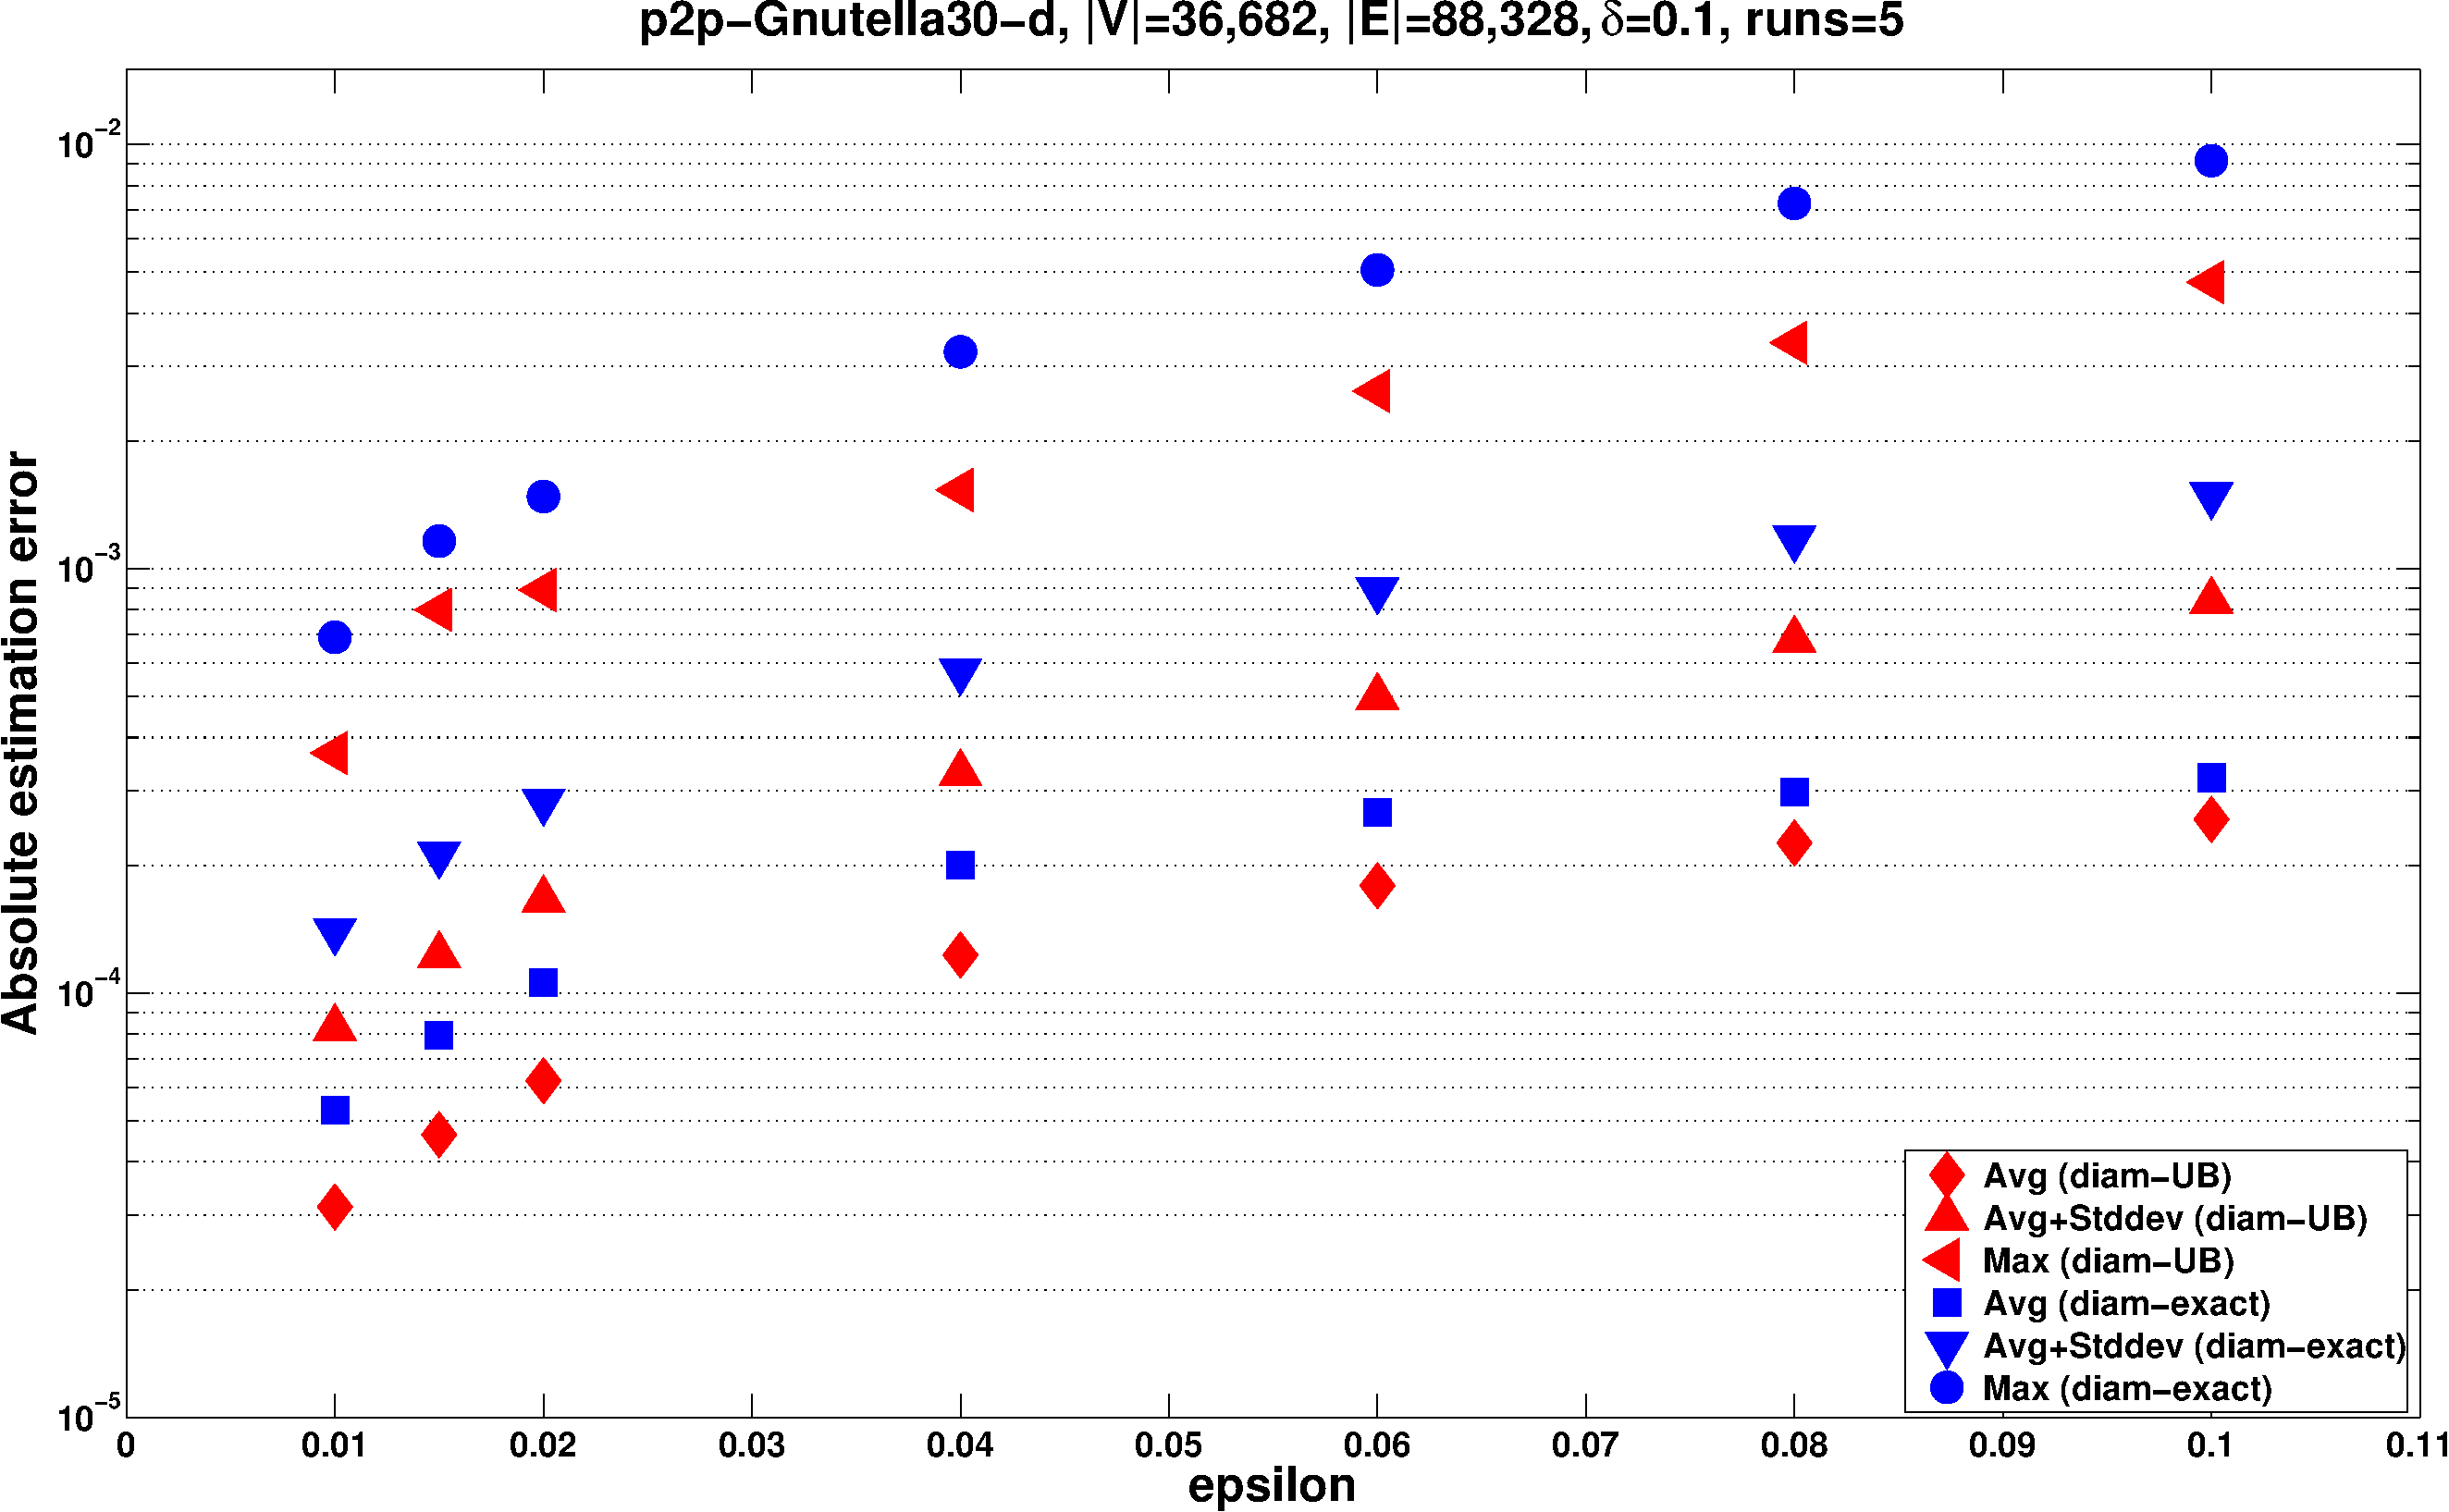
\includegraphics[width=\textwidth]{centrsampl/figures/eps/p2p-Gnutella30-error}
    \caption{p2p-Gnutella30 (directed)}
    \label{fig:centrsamplgnutella:error}
  \end{subfigure}
  \ifproof
  \hfill
  \begin{subfigure}[b]{0.49\textwidth}
    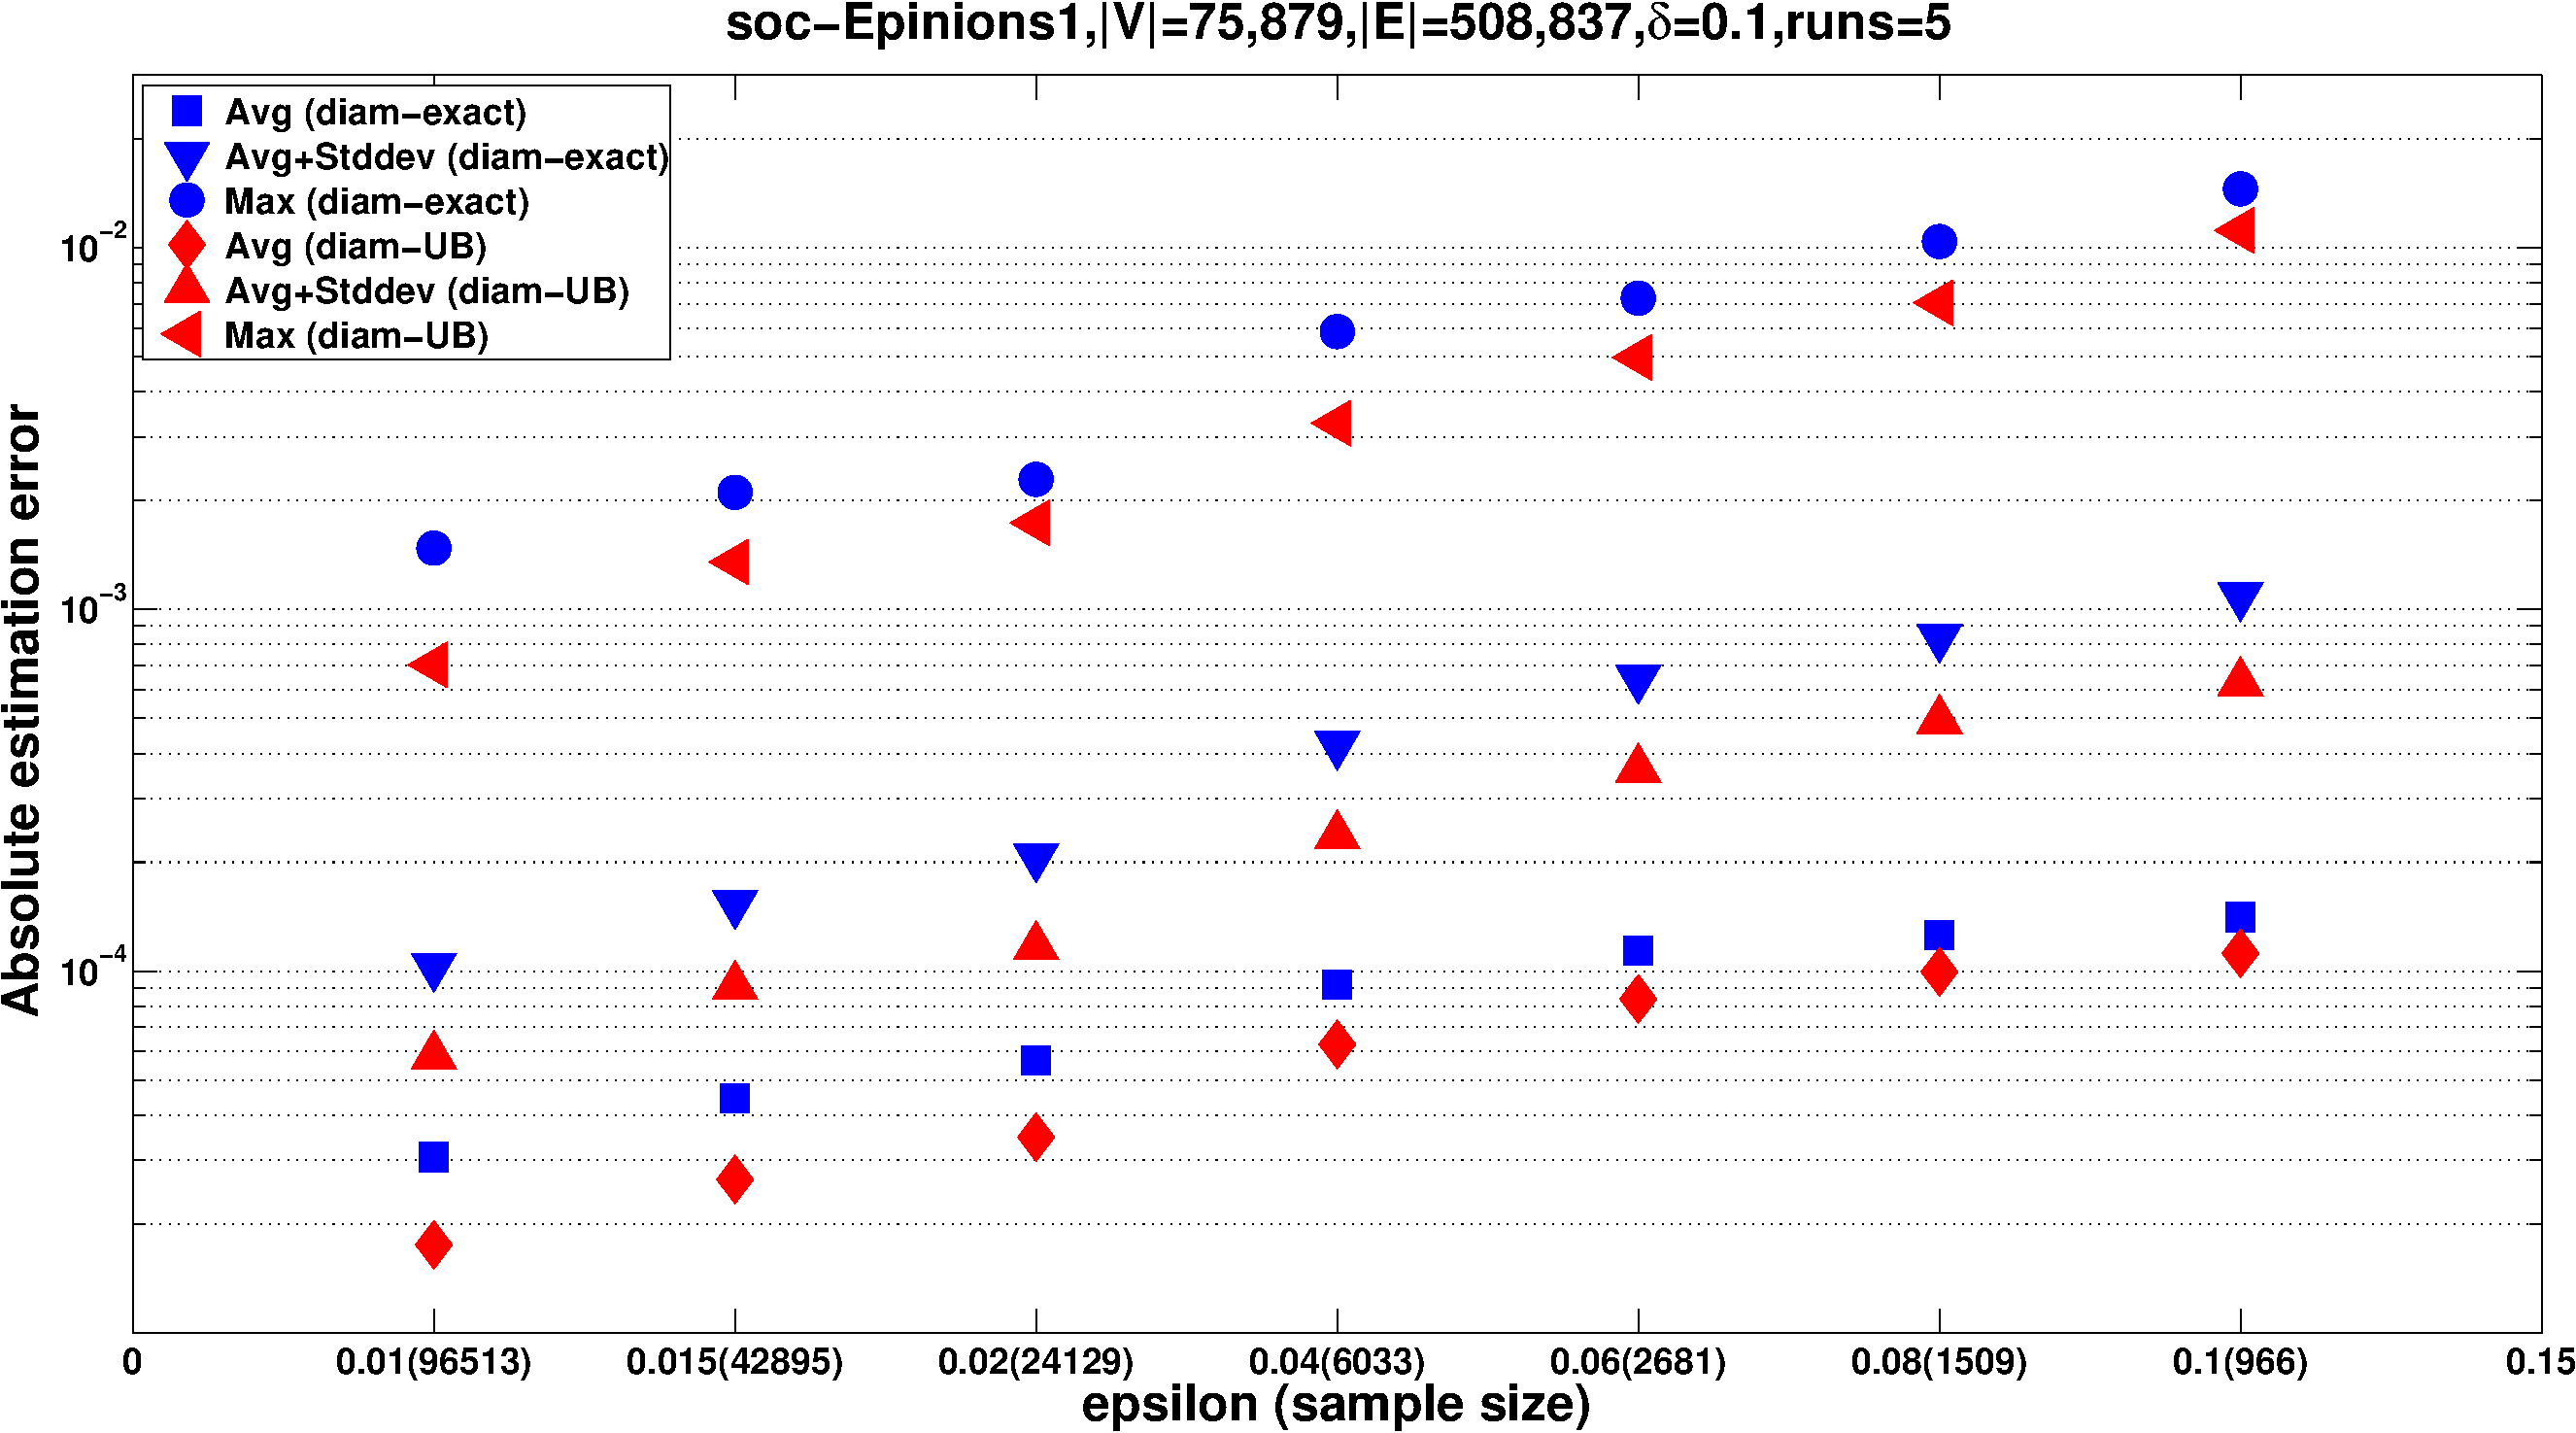
\includegraphics[width=\textwidth]{centrsampl/figures/eps/soc-Epinions1-error}
    \caption{soc-Epinions1 (directed)}
    \label{fig:centrsamplEpinions:error}
  \end{subfigure}

  \begin{subfigure}[b]{0.49\textwidth}
    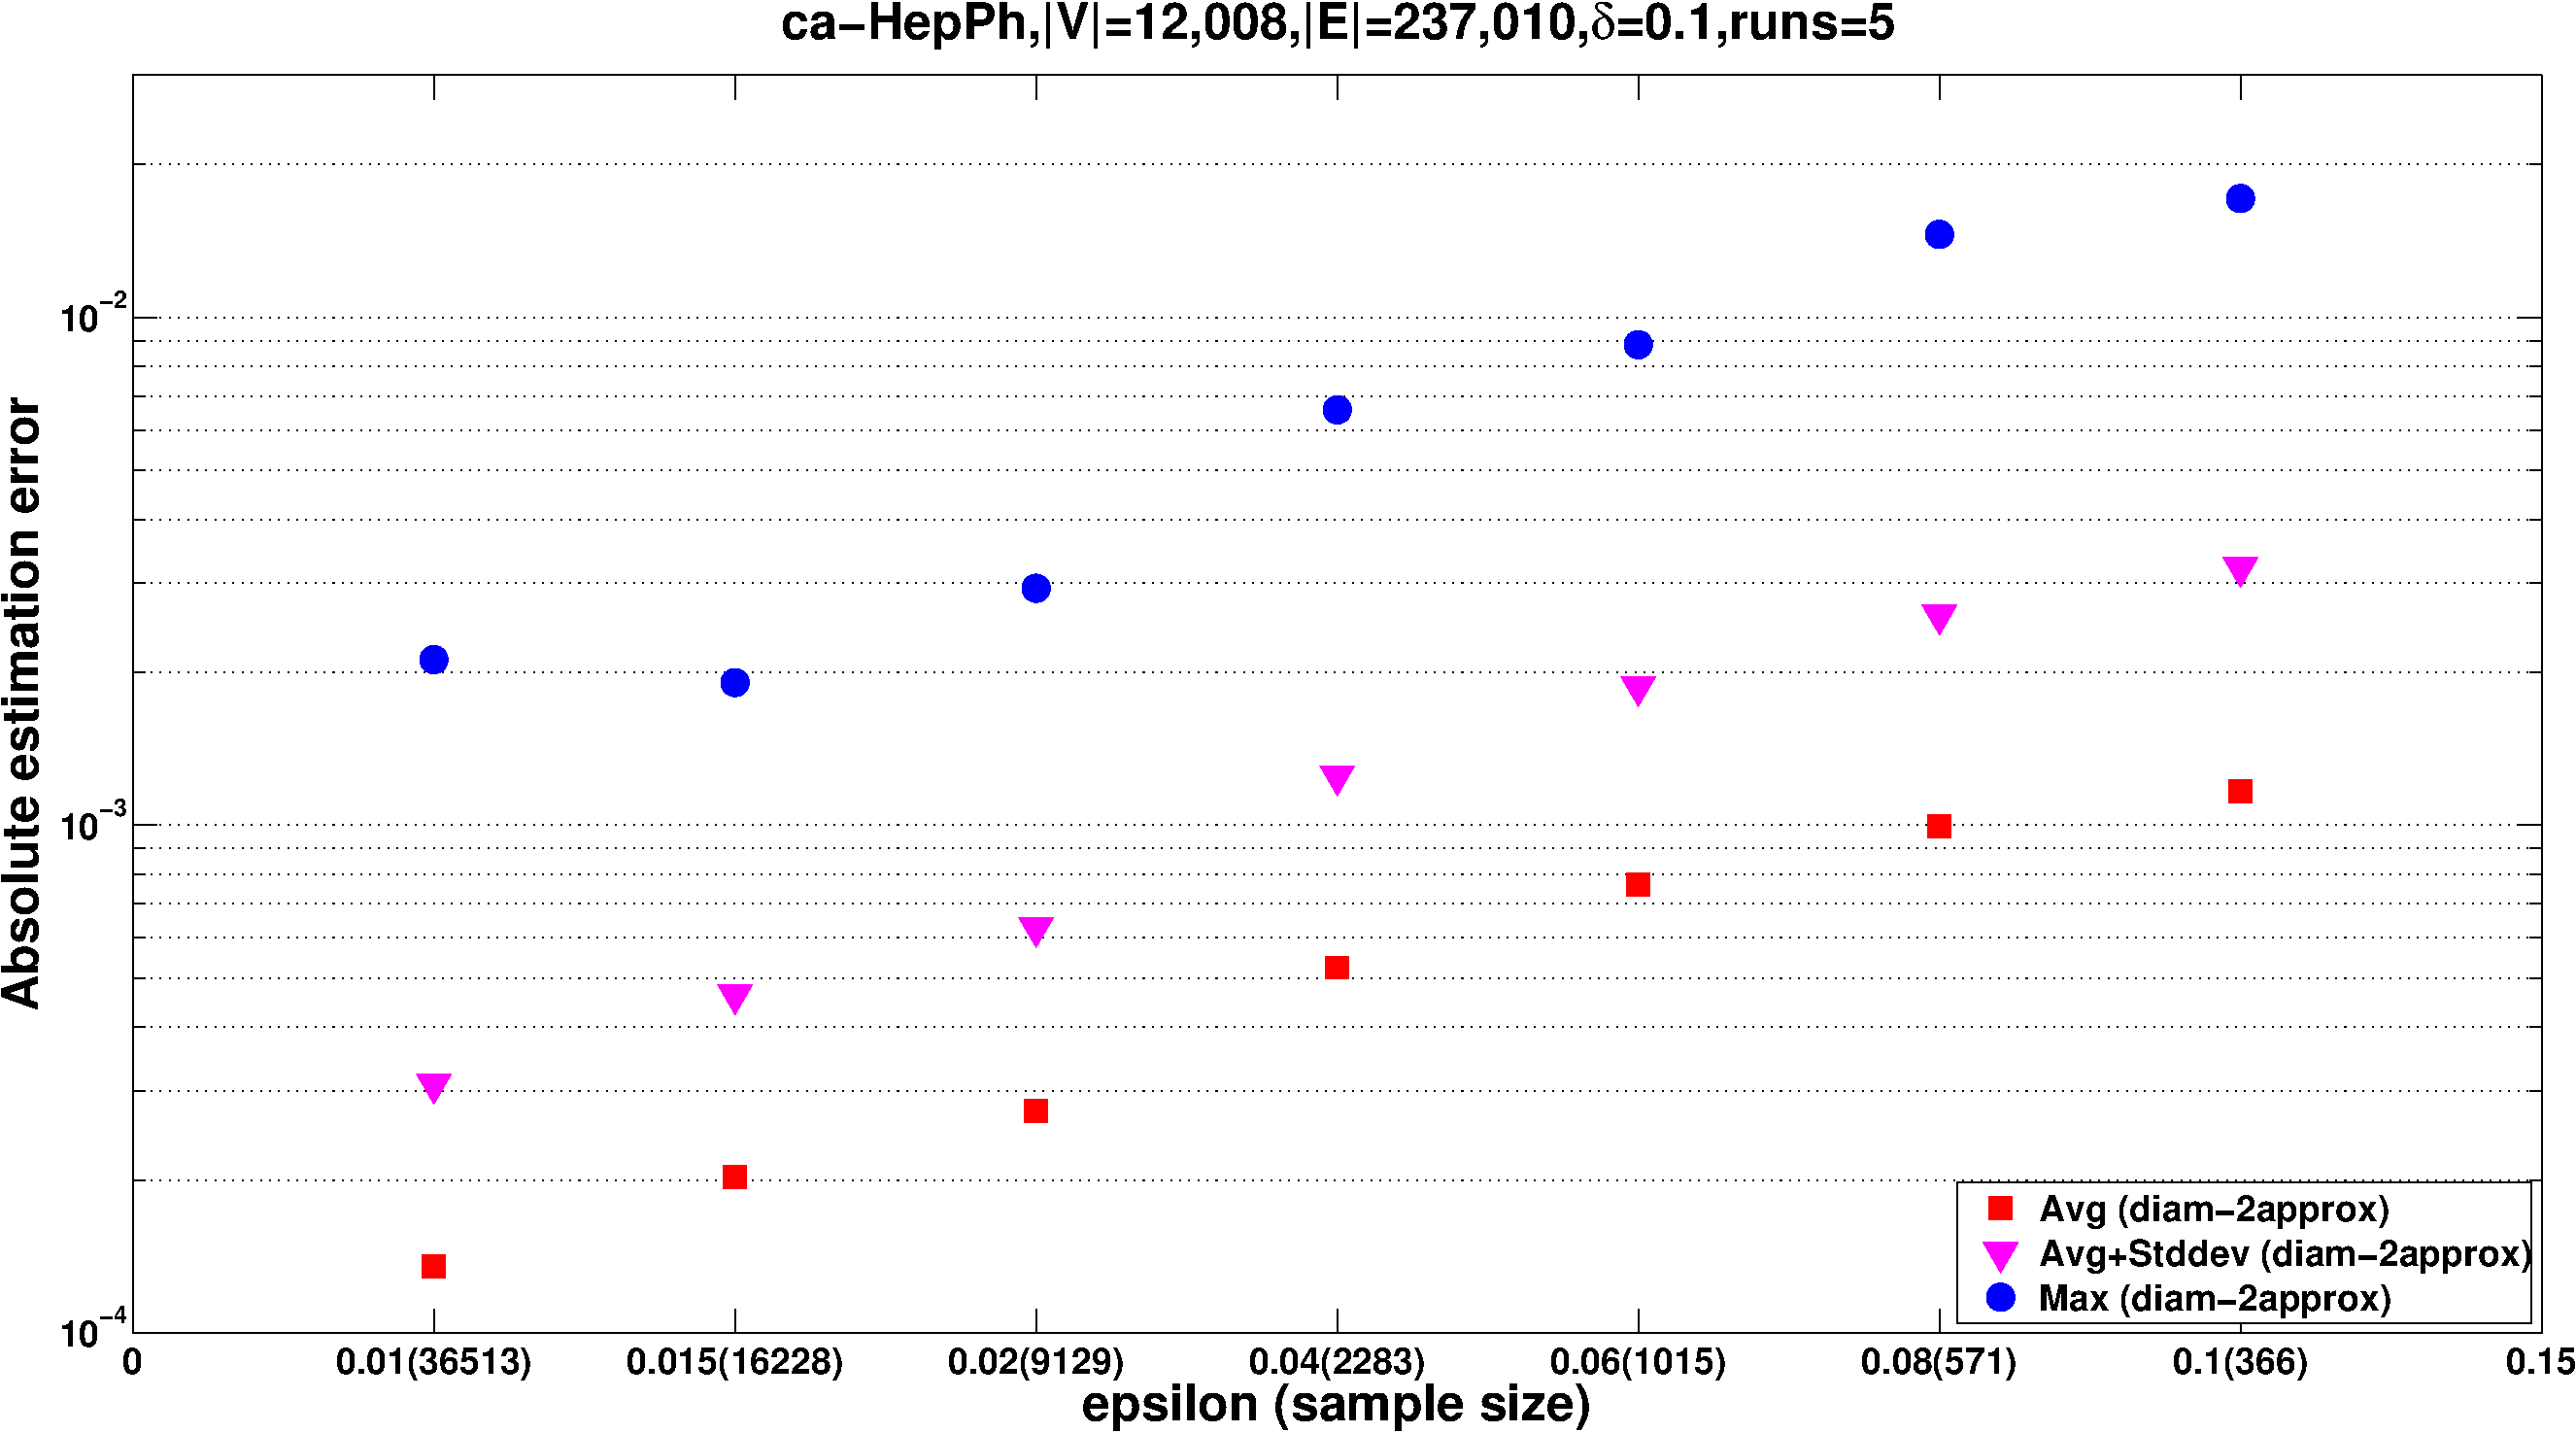
\includegraphics[width=\textwidth]{centrsampl/figures/eps/ca-HepPh-error}
    \caption{ca-HepPh (directed)}
    \label{fig:centrsamplHepPh:error}
  \end{subfigure}
  \fi
  \hfill
  \begin{subfigure}[b]{0.49\textwidth}
    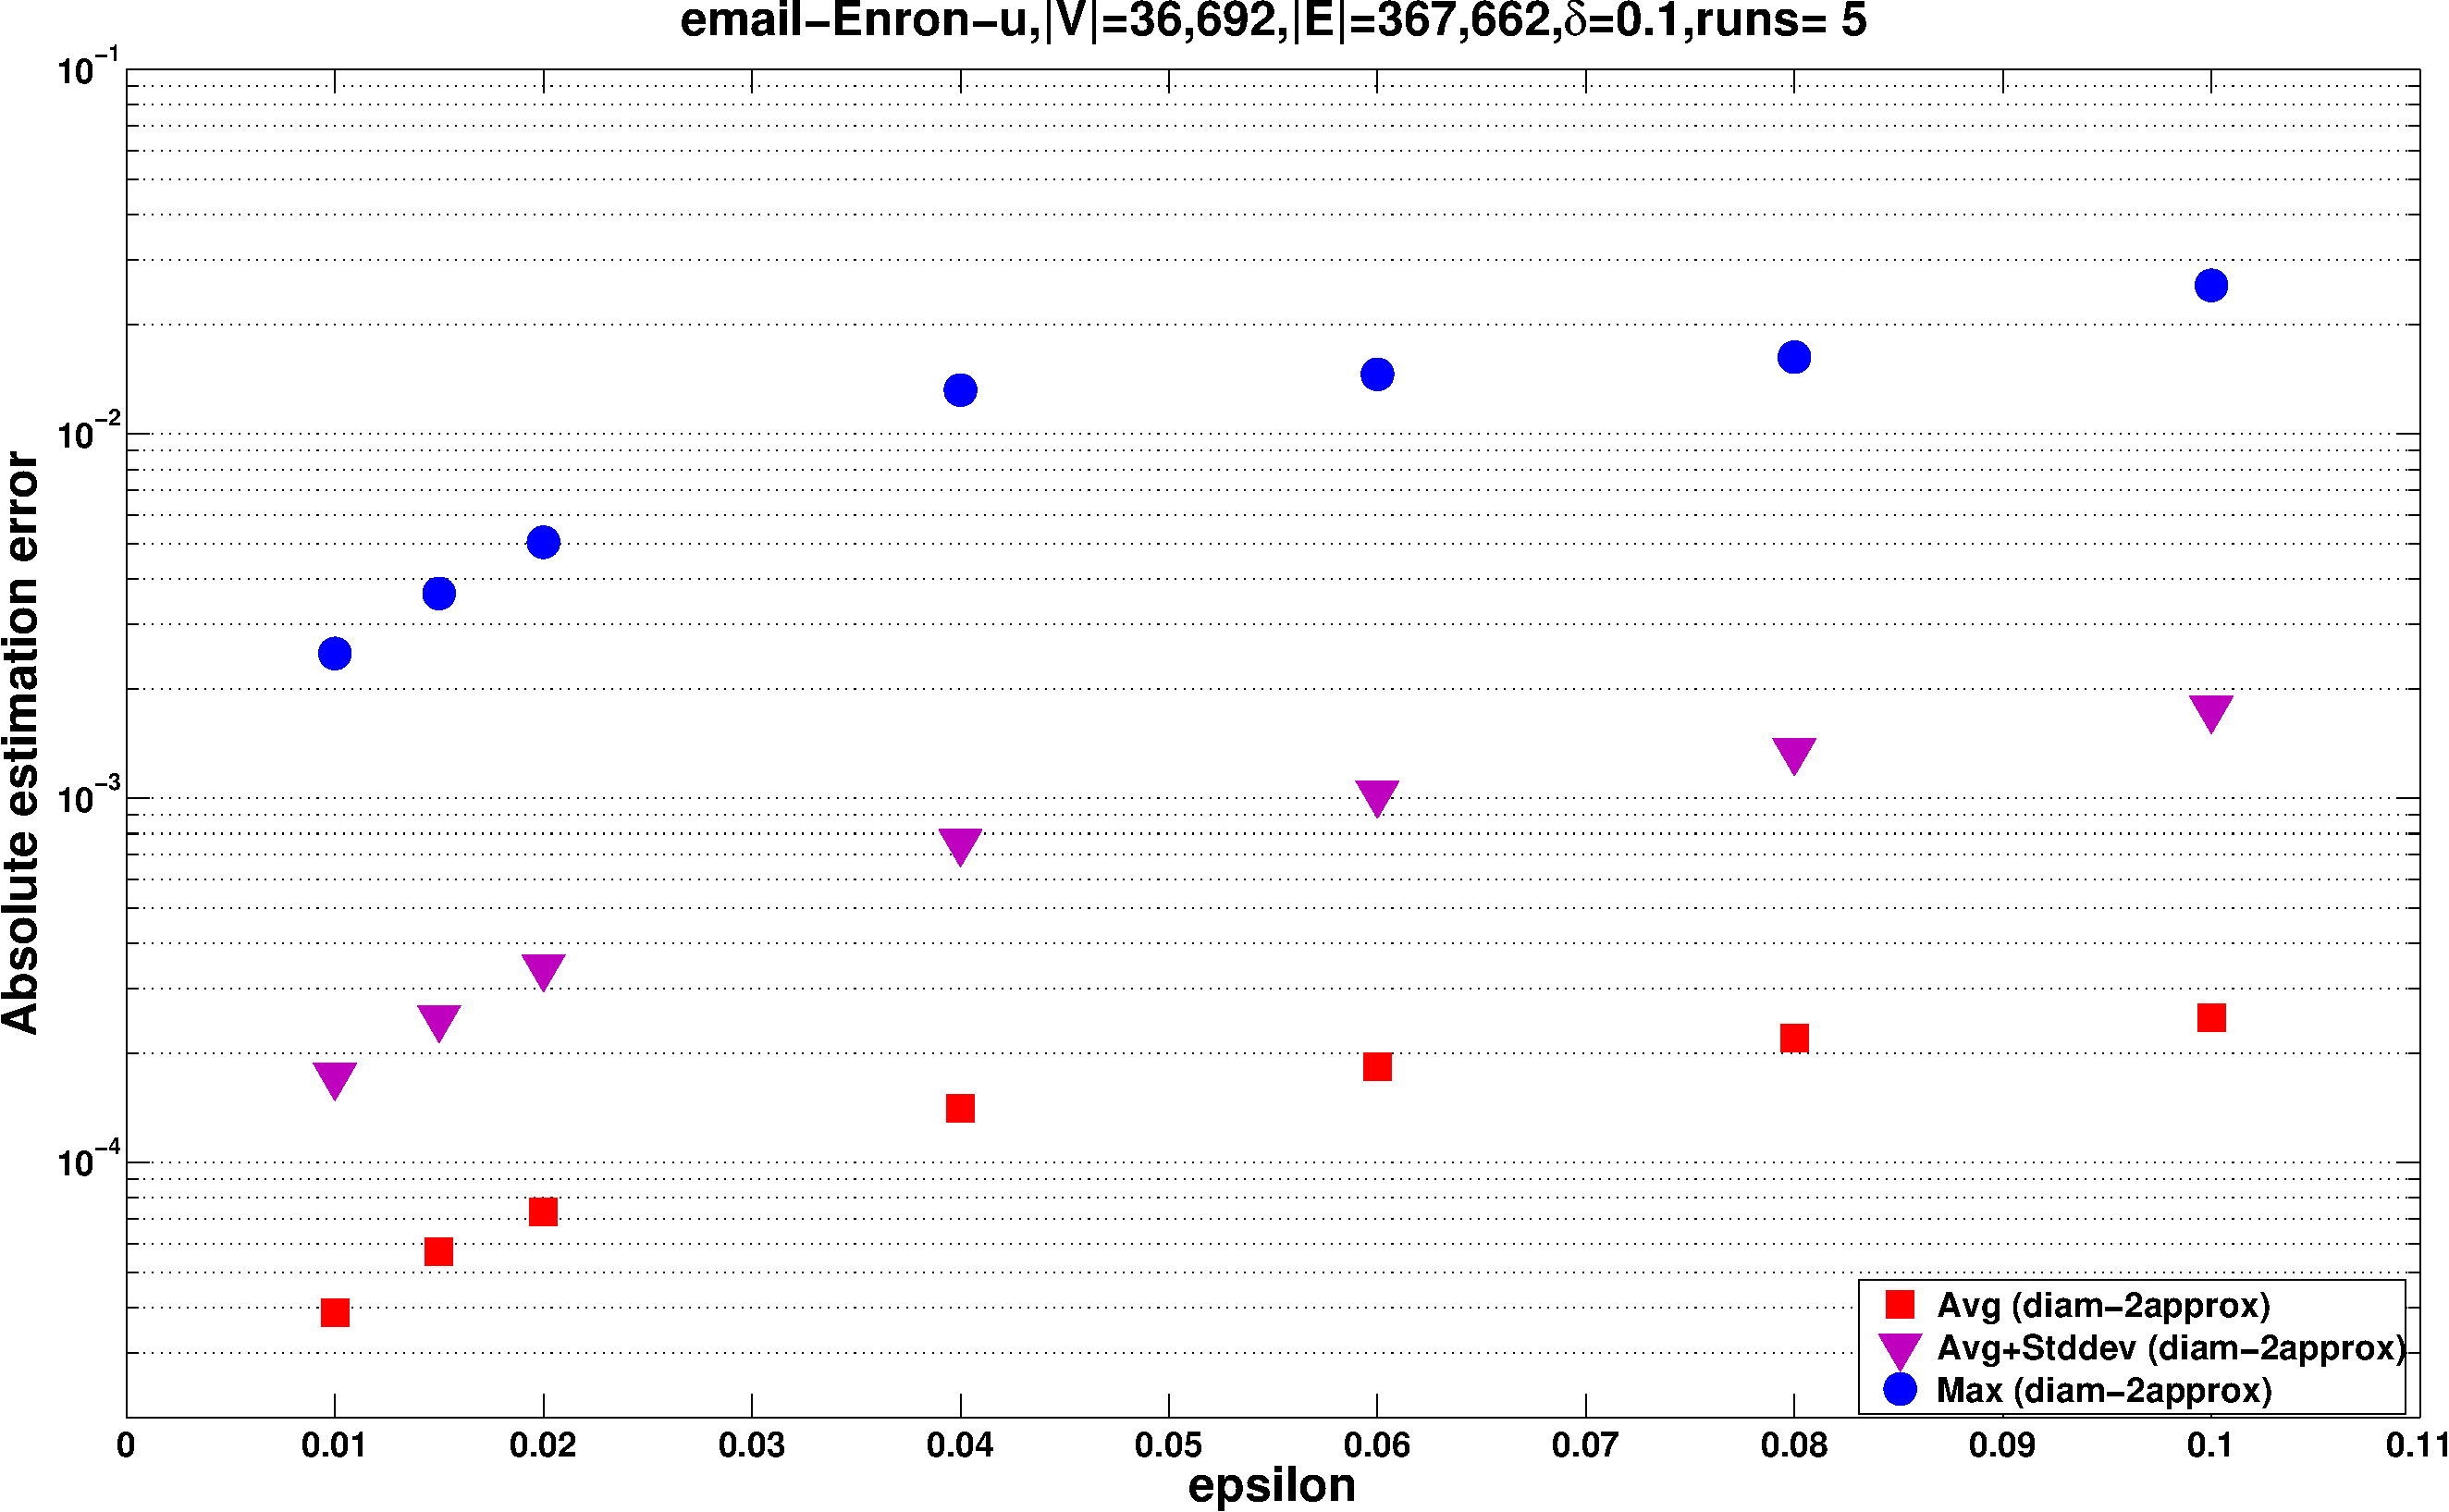
\includegraphics[width=\textwidth]{centrsampl/figures/eps/email-Enron-error}
    \caption{email-Enron (undirected)}
    \label{fig:centrsamplemail:error}
  \end{subfigure}
  \caption{Betweenness estimation error $|\tilde\betw(v)-\betw(v)|$ evaluation for directed and undirected graphs} 
  \label{fig:centrsamplerror}
\end{figure}

\begin{figure}[ht]
  \centering
  \begin{subfigure}[b]{0.49\textwidth}
    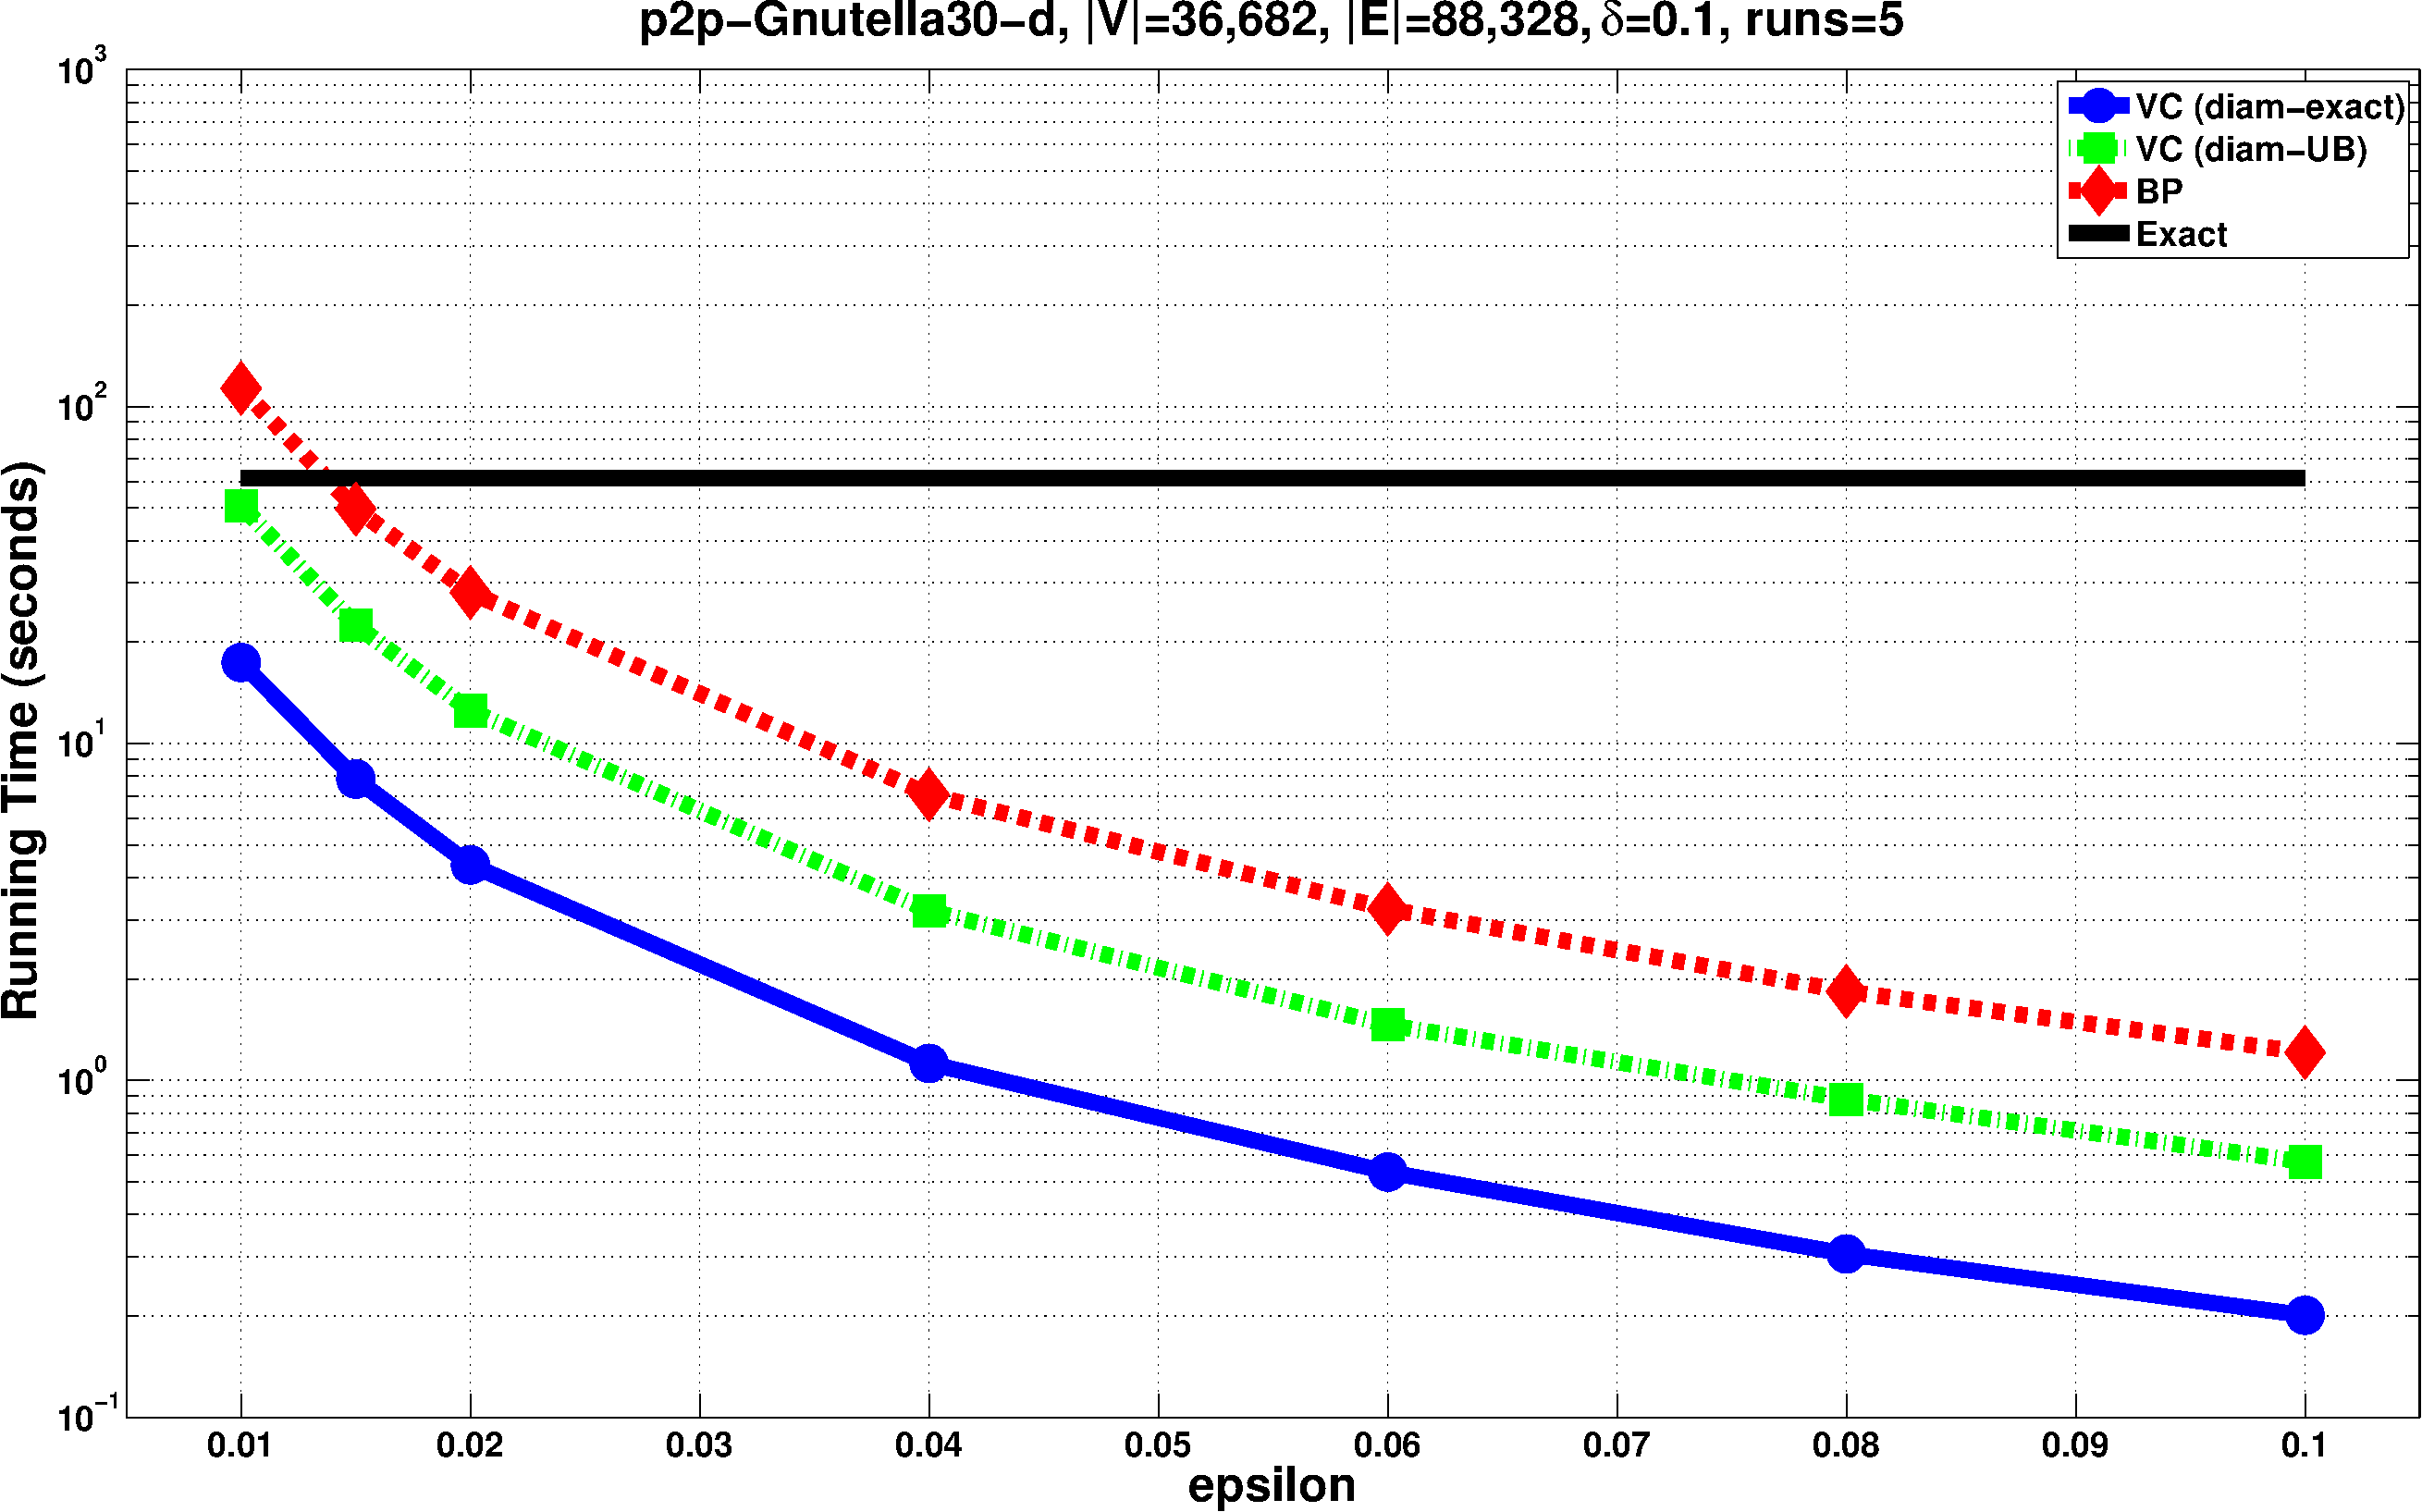
\includegraphics[width=\textwidth]{centrsampl/figures/eps/p2p-Gnutella30-time}
    \caption{p2p-Gnutella30 (directed)}
    \label{fig:centrsamplgnutella:time}
  \end{subfigure}
  \ifproof
  \hfill
  \begin{subfigure}[b]{0.49\textwidth}
    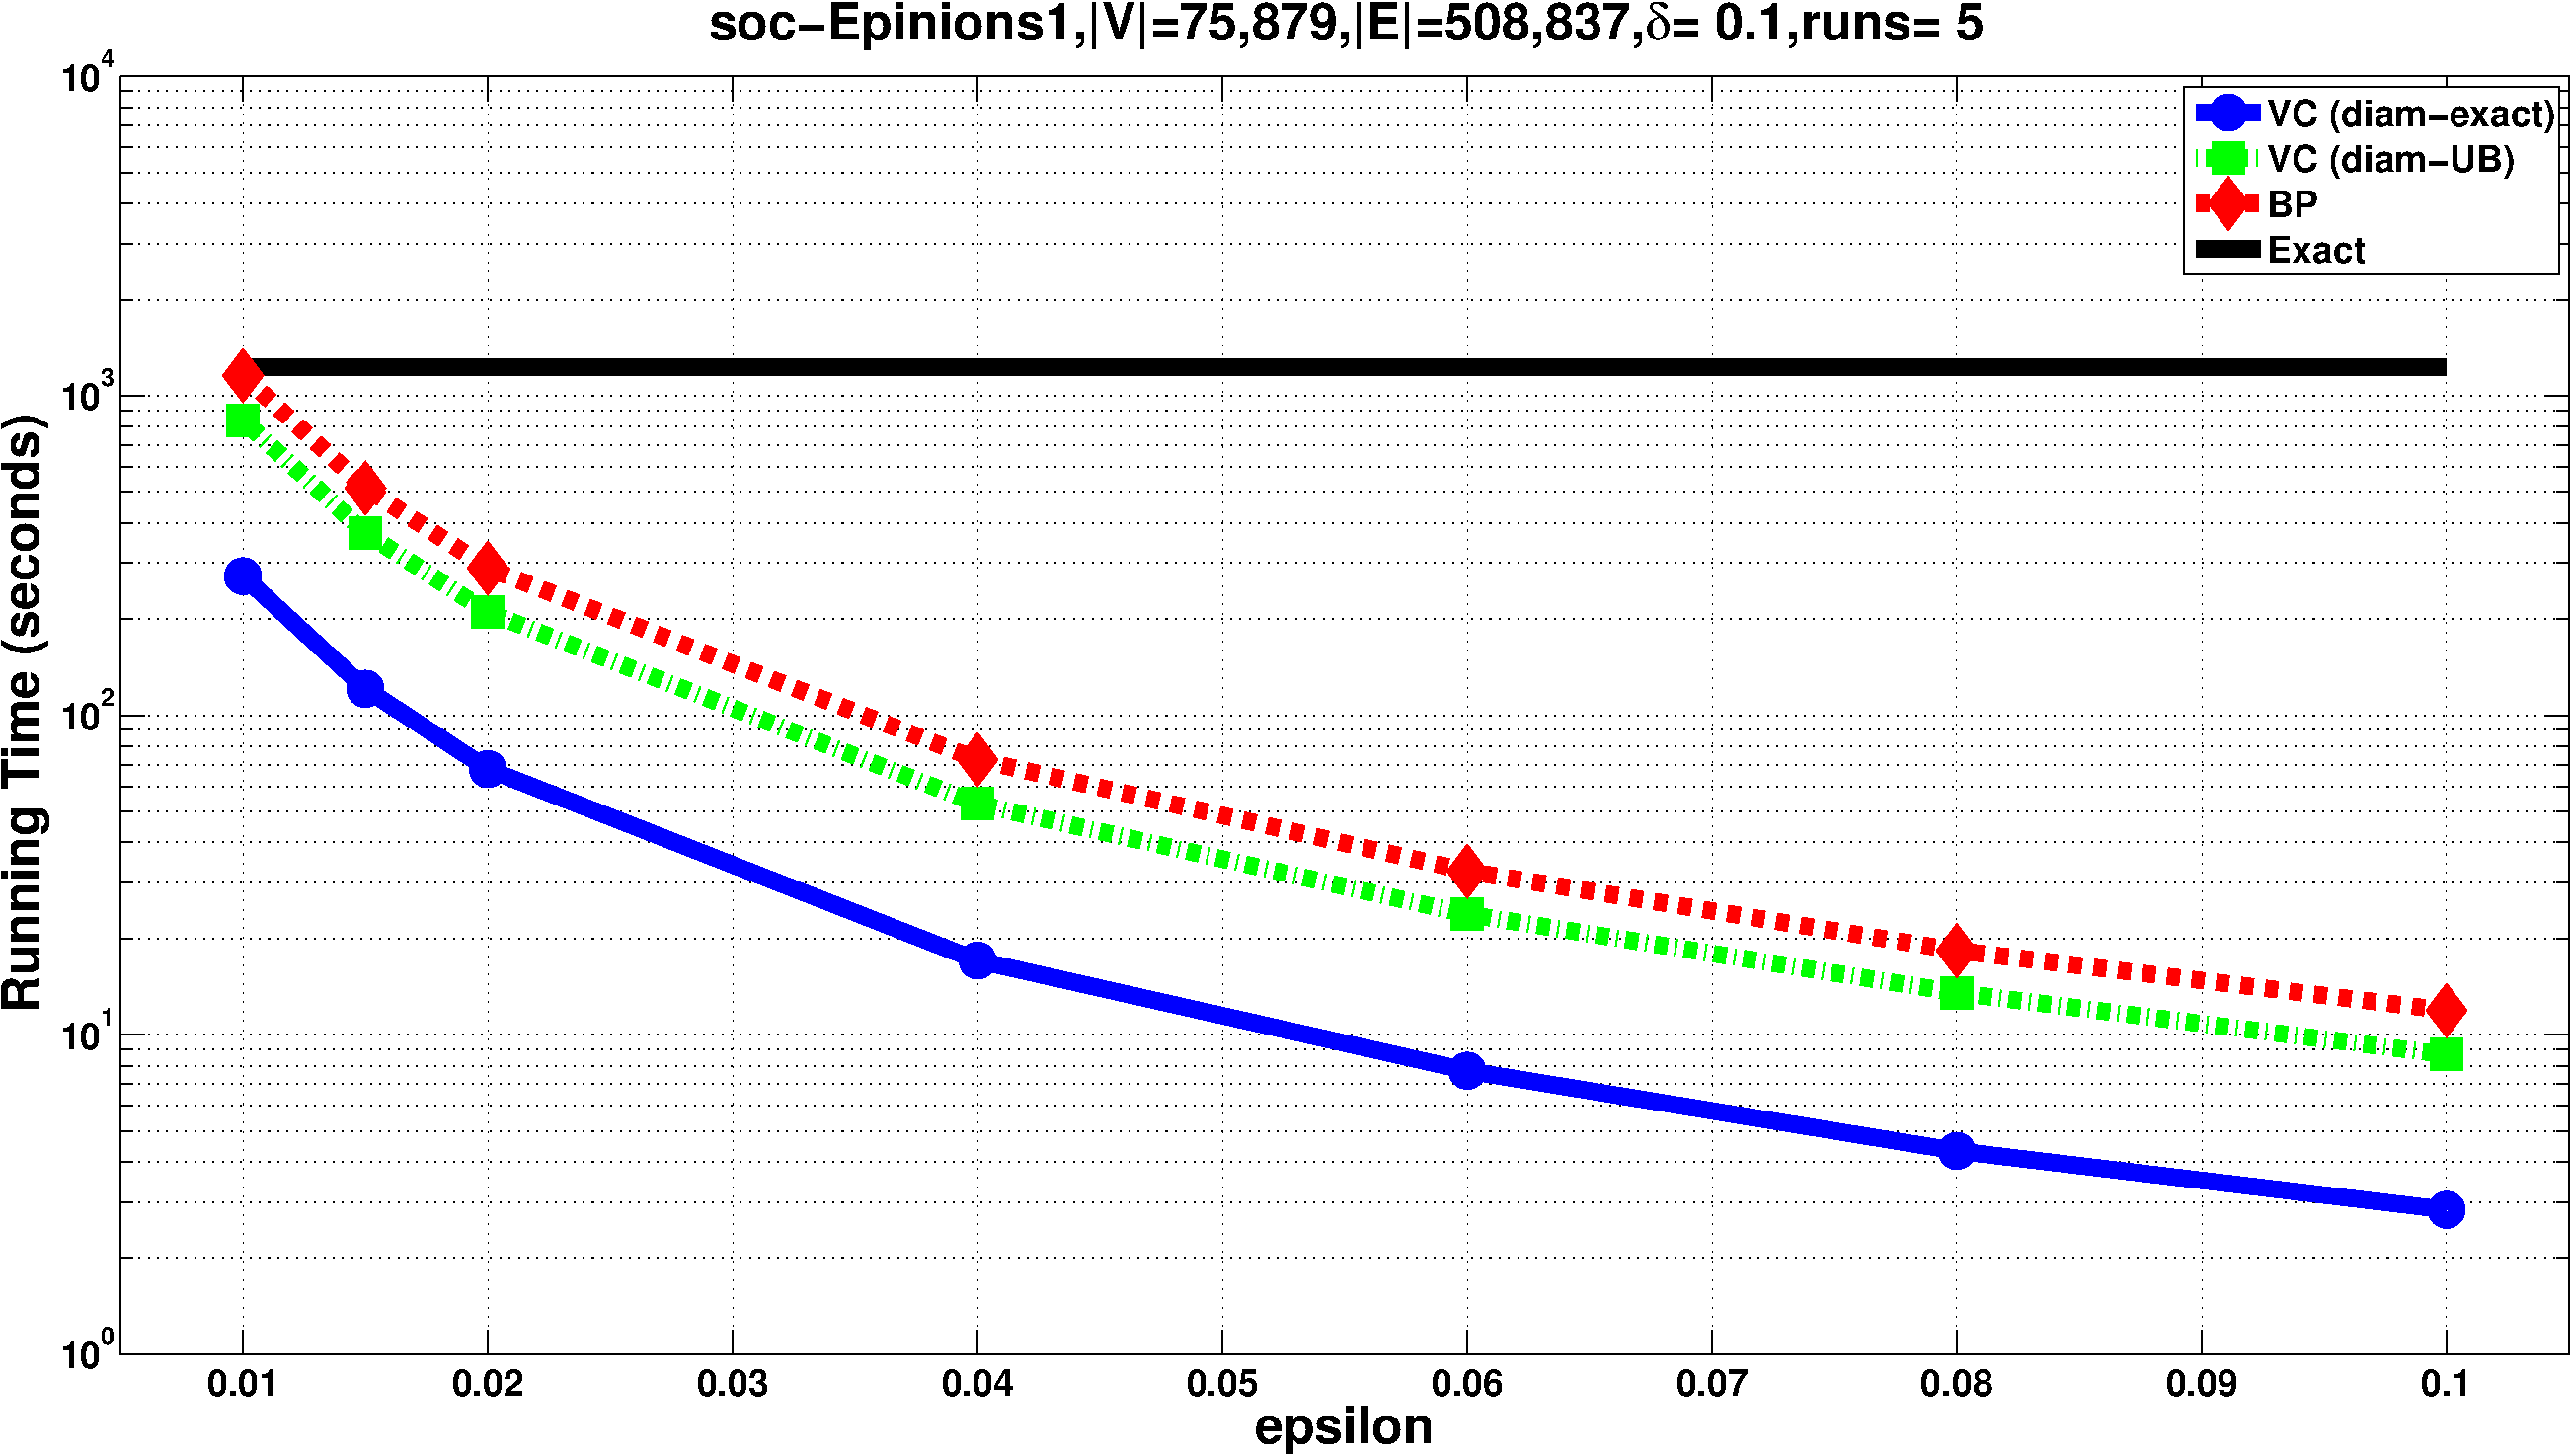
\includegraphics[width=\textwidth]{centrsampl/figures/eps/soc-Epinions1-time}
    \caption{soc-Epinions1 (directed)}
    \label{fig:centrsamplEpinions:time}
  \end{subfigure}

  \begin{subfigure}[b]{0.49\textwidth}
    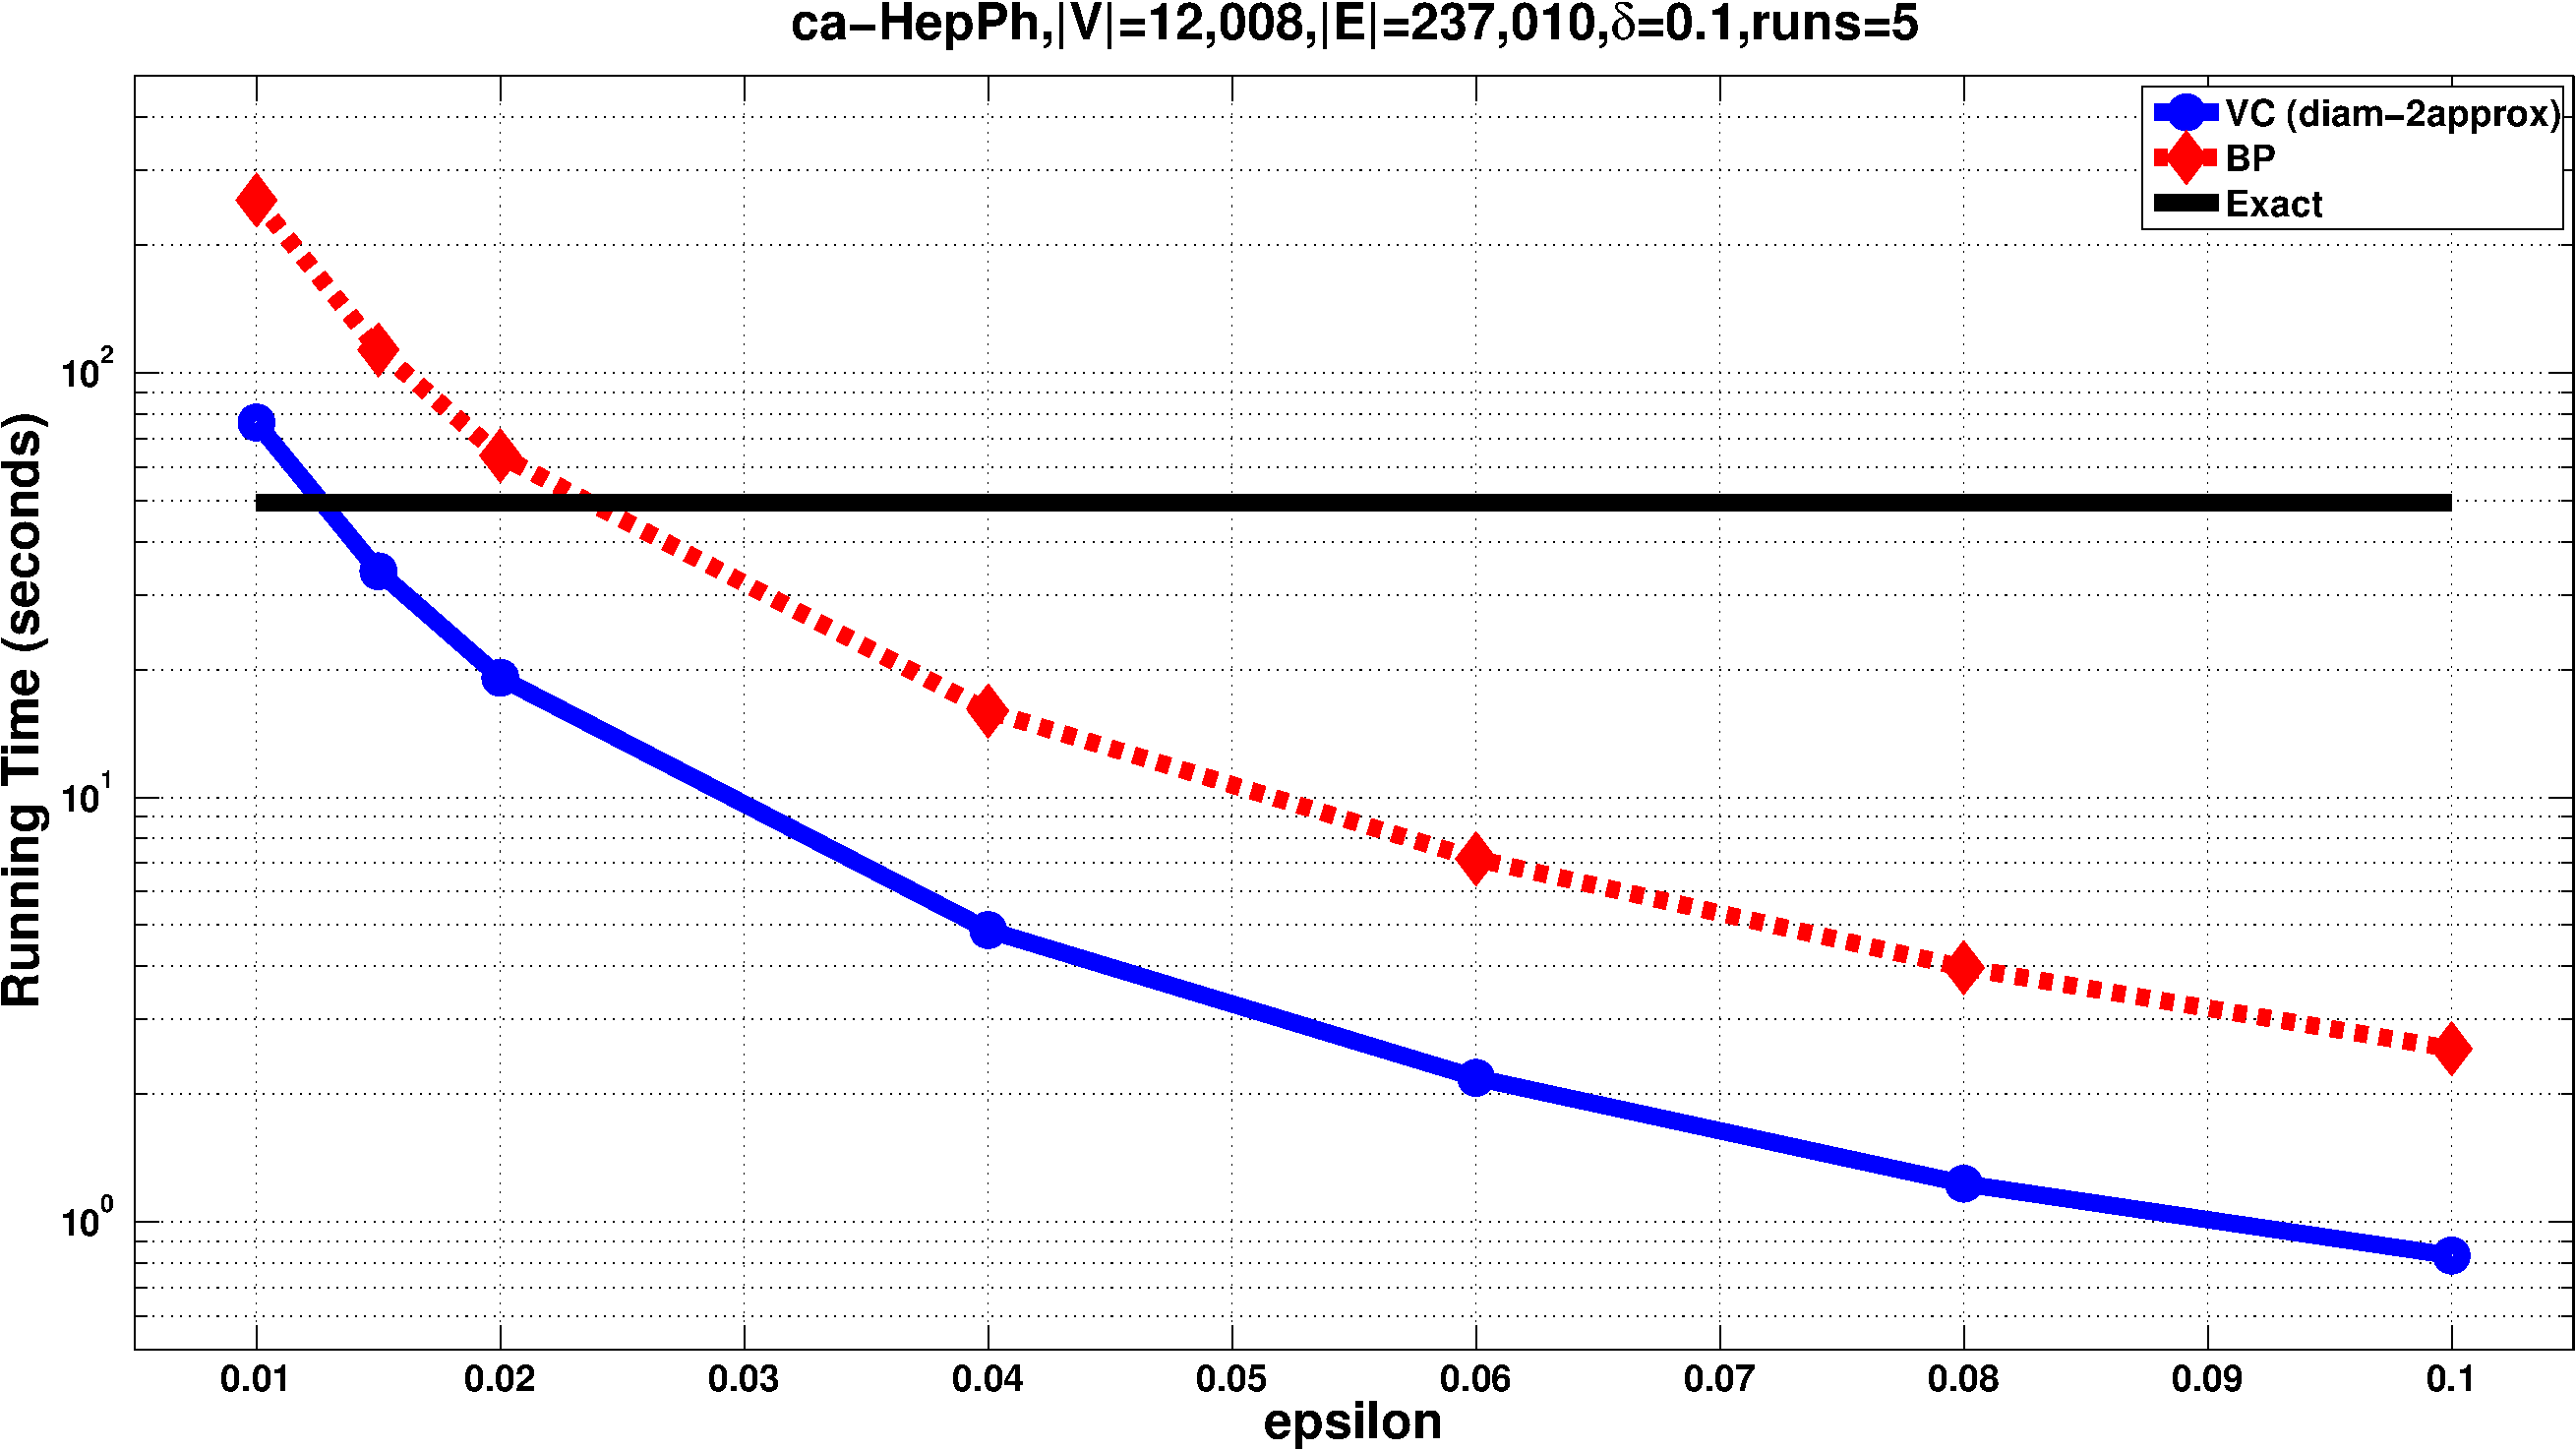
\includegraphics[width=\textwidth]{centrsampl/figures/eps/ca-HepPh-time}
    \caption{ca-HepPh (directed)}
    \label{fig:centrsamplHepPh:time}
  \end{subfigure}
  \fi
  \hfill
  \begin{subfigure}[b]{0.49\textwidth}
    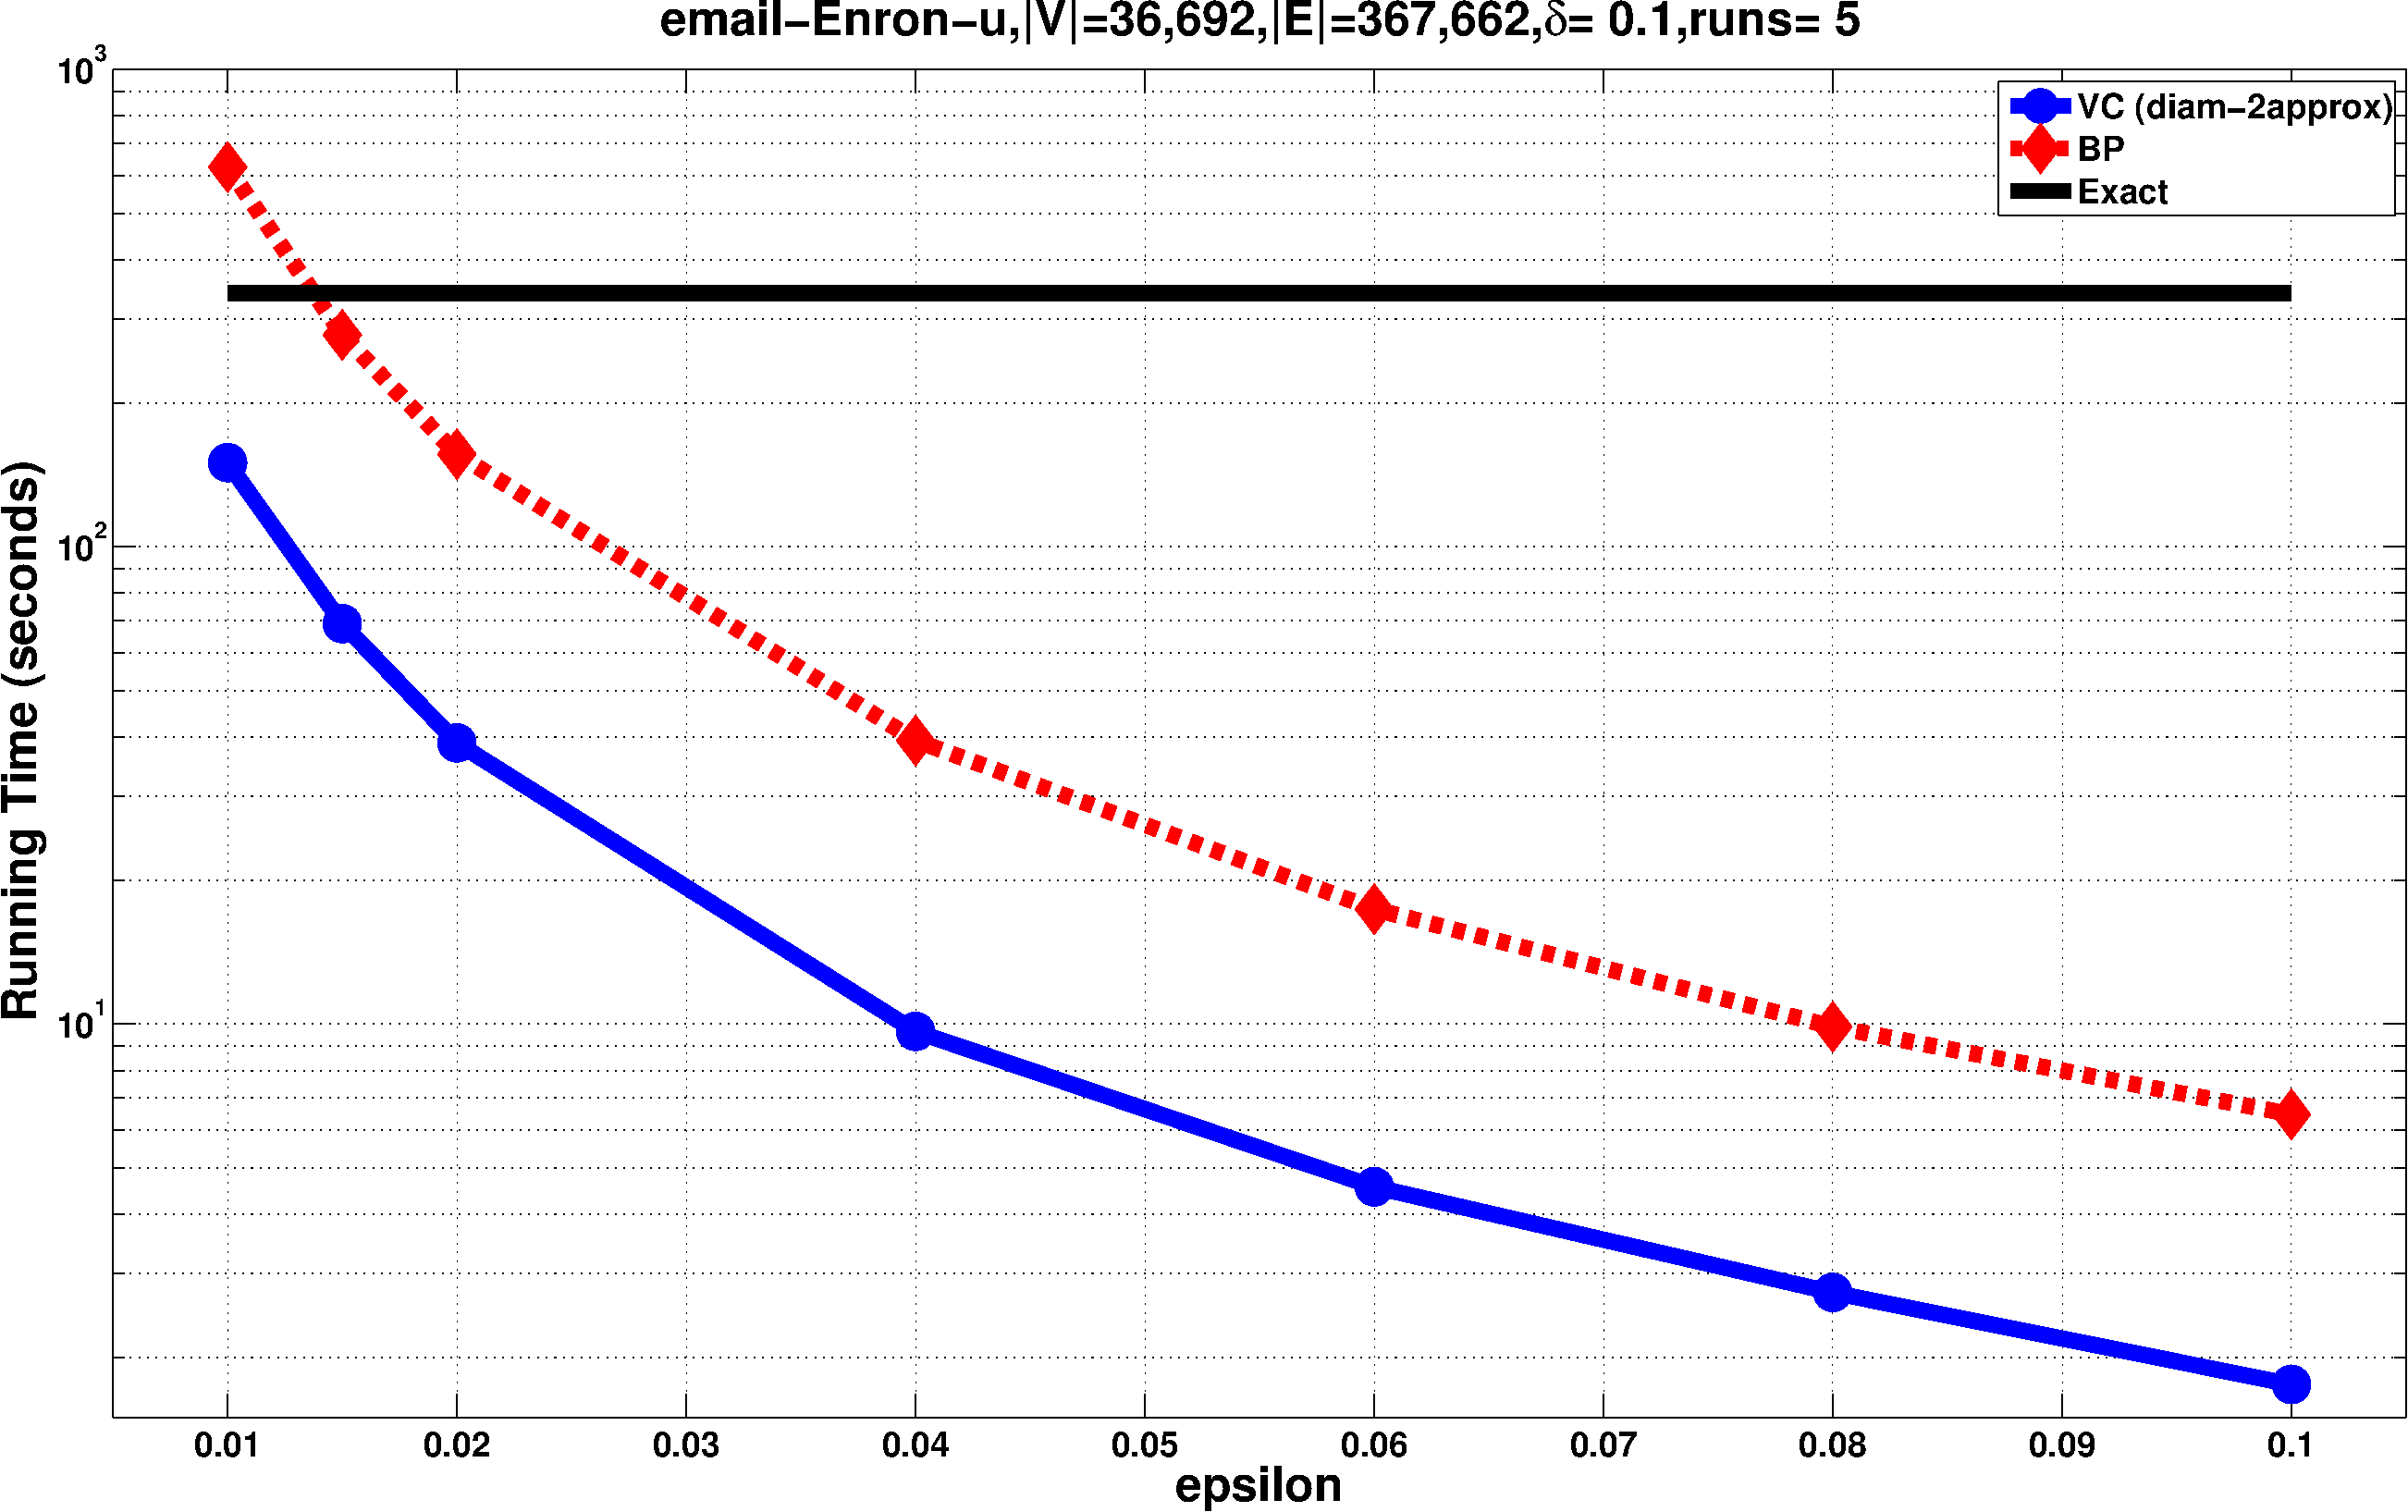
\includegraphics[width=\textwidth]{centrsampl/figures/eps/email-Enron-time}
    \caption{email-Enron (undirected)}
    \label{fig:centrsamplemail:time}
  \end{subfigure}
  \caption{Running time (seconds) comparison between $\mathsf{VC}$, $\mathsf{BP}$, and the
  exact algorithm.}
  \label{fig:centrsampltime}
\end{figure}

\subsection{Runtime}\label{sec:centrsamplruntime}
We compared the running time of Algorithm~\ref{alg:algorithm} (denoted in the
following as $\mathsf{VC}$ to that of the algorithm
from~\citep{JacobKLPT05,BrandesP07,GeisbergerSS08}
(denoted as $\mathsf{BP}$), and to that of the exact
algorithm~\citep{Brandes01}. As $\mathsf{VC}$ and $\mathsf{BP}$ give the same
guarantees on the accuracy and confidence of the computed estimations, it makes
sense to compare their running times to evaluate which is faster in achieving
the goal. The performances of the algorithm proposed in~\citep{GeisbergerSS08}
takes the same time as $\mathsf{BP}$, because it follows the same sampling
approach and only differs in the definiton of the estimator for the betweenness,
so we do not report those.
%as the one
%from~\citep{BrandesP07,JacobKLPT05} and only differs in the definition of the
%estimator for the betweenness of a vertex. Because of this, it takes the same
%amount of time and touches the same number of edges as the one
%from~\citep{BrandesP07}.
%We use two metrics in order to measure the amount of computations that the
%algorithms perform. The first metric is the execution time, or \textit{time}, in
%seconds, the second metric is the number of edges that the algorithm
%touched/traversed, or \textit{touched edges}, during the execution. The number
%of touched edges is a graph theoretic metric \XXX What do you mean by that? that
%does not depend on the specifications of the implementation environment and
%gives a perspective of the amount of work that the algorithm requires. It is
%worth mentioning that we count an edge as many times as it is touched during
%a run of an algorithm, so we might count a single edge more than once.
The algorithms $\mathsf{VC}$ and $\mathsf{BP}$ take parameters $\varepsilon$ and
$\delta$ and compute the sample size accordingly. 
%For our experiments we used
%$\delta=0.1$, while $\varepsilon$ takes value in $\{0.01, 0.015, 0.02, 0.04,
%0.06, 0.08, 0.1\}$.
 We run each experiments five times for each value of $\varepsilon$, and
measured the average running time across the runs.
%as well as the average number of touched edges.  
The results are presented in Figs.~\ref{fig:centrsampltables} 
%and~\Cref{fig:centrsamplgnutella:time,fig:centrsamplgnutella:edges,fig:centrsamplemail:time,fig:centrsamplemail:edges}.
and~\ref{fig:centrsampltime}. 
%
In Fig.~\ref{tab:expUndir} we report the minimum and the maximum ratio of the
running time of $\mathsf{BP}$ over $\mathsf{VC}$, taken over the ratios obtained
by running the algorithms with the different values of $\varepsilon$. As it can
be seen from this table our algorithm performs significantly faster, more than
300\%. Similar results are reported for directed graphs in Fig.~\ref{tab:expDir}.
%In~\Cref{tab:expDir} we compare the
%algorithms on a set of directed graphs. As in the case of the undirected graphs,
%we present the minimum and maximum ratios of corresponding measures for the
%different values of $\varepsilon$. 
The diam-UB
and the diam-exact values can be seen as the two extremes for the performance of 
Algorithm~\ref{alg:algorithm} in terms of runtime. In the case of the diam-exact
we have as few samples as possible (for $\mathsf{VC}$) since we use the exact
value of the vertex-diameter, whereas in the case of diam-UB we have as many
samples as possibles because we use the worst case estimation for the
vertex-diameter of the graph.  %(that is when the graph has a hamiltonian path) <= not correct.  
From Fig.~\ref{tab:expUndir} we can see that the value for the
vertex-diameter that we consider in the case of diam-UB $(|V|-2)$ is many orders of
magnitudes greater than the actual value, which translates in a significant
increase of the number of samples. But even in the case of this crude
vertex-diameter approximation (diam-UB), the $\mathsf{VC}$ algorithm performs uniformly faster than
$\mathsf{BP}$. In the case where the exact value of the diameter was used, we
can see that our algorithm computes an estimation of the betweenness that
satisfies the desired accuracy and confidence guarantees \emph{3 to 5 times
faster} than~$\mathsf{BP}$. 
%\XXX-(COMMENT ON THE RELATION TOPOLOGY-SPEED) \MR I have no idea what you meant by that. 
 In Fig.~\ref{fig:centrsamplgnutella:time} we study
the directed graph p2p-Gnutella30 and we present the measurements of
the average running time of the algorithms for different values of
$\varepsilon$, using the exact algorithm from~\citep{Brandes01} as baseline. The
$\mathsf{VC}$ algorithm requires significantly less time than the $\mathsf{BP}$
algorithm. The figure also shows that there are values of $\varepsilon$ for
which $\mathsf{BP}$ takes more time than the exact algorithm, because the
resulting sample size is larger than the graph size. Given that $\mathsf{VC}$
uses fewer samples and does fewer operations per sample, it can be used with
lower $\varepsilon$ than $\mathsf{BP}$, while still saving time compared to the
exact computation. Figure~\ref{fig:centrsamplemail:time} shows the average running time of the
algorithms for the undirected graph email-Enron. The behavior is  similar to
that for the undirected case. %In this case our
%algorithm not only performs better but also \emph{scales} better than the one
%from~\citep{BrandesP07} \XXX WHAT DO YOU MEAN SCALES BETTER?. 
%For the computation of the sample size we use the 2-approximation algorithm
%which is enough since what we really use for the computation of sample size is
%the logarithm of the diameter. 
%In~\Cref{fig:centrsamplgnutella:edges,fig:centrsamplemail:edges}, we study the average number of
%touched edges for the case of the directed graph \texttt{p2p-Gnutella30} and of
%the undirected graph \texttt{email-Enron} respectively. It is evident that again
%our algorithm outperforms $\mathsf{BP}$. 
%From the above Figures and Tables we see that for the tested values of
%$\varepsilon$, the proposed algorithm is faster (at least 3x speedup in case of
%exact diameter on the tested graphs). 
 Algorithm~\ref{alg:algorithm} is faster than $\mathsf{BP}$ for two reasons, both
originating from from our use of results from the VC-dimension theory: 1) we use
a significantly smaller amount of samples and 2) $\mathsf{VC}$ performs the
same amount of computations \emph{per sample} as $\mathsf{BP}$ only in the worst
case. Indeed our algorithm needs only to find the shortest path between a
sampled pair of vertices, whereas the algorithms
from~\citep{GeisbergerSS08,BrandesP07} need to compute the shortest paths
between a sampled source and all the other vertices. In our experimental
evaluation we found out that the running time of the algorithms is directly
proportional to the number of edges touched during the shortest path
computation. The use of bidirectional A\textsuperscript{*}
search~\citep{Pohl69,KaindlK97} can help in lowering the number of touched edges
for $\mathsf{VC}$ and therefore the runtime of our algorithm ($\mathsf{BP}$
would not benefit from this improvement). This is a possible direction for
future research. 
%\begin{figure}[ht]
%  \centering
%  \hfill
%  \subfloat[p2p-Gnutella30
%  (directed)]{\label{fig:centrsamplgnutella:edges}\includegraphics[width=.45\textwidth,keepaspectratio]{p2p-Gnutella30-edges}}
%  \hfil
%  \subfloat[email-Enron
%  (undirected)]{\label{fig:centrsamplemail:edges}\includegraphics[width=.45\textwidth,keepaspectratio]{email-Enron-edges}}
%  \hfill
%  \label{fig:centrsampledges}
%  \caption{Touched edges comparison between $\mathsf{VC}$, $\mathsf{BP}$, and
%  the exact algorithm.}
%\begin{minipage}[b]{0.5\linewidth}
%\flushleft
%\includegraphics[width=3.8in, keepaspectratio]{p2p-Gnutella30-edges.eps}
%\caption{Touched edges comparison on p2p-Gnutella30} \label{fig:centrsamplgnutella:edges}
%\end{minipage}%
%\begin{minipage}[b]{0.5\linewidth}
%\centering
%\includegraphics[width=3.8in, keepaspectratio]{email-Enron-edges.eps}
%\caption{Touched edges comparison on email-Enron}\label{fig:centrsamplemail:edges}
%\end{minipage}
%\end{figure}

\subsection{Scalability}\label{sec:centrsamplscalability}

In Sect.~\ref{sec:centrsampldiscussion} we argued about the reasons why
Algorithm~\ref{alg:algorithm} is more scalable than $\mathsf{BP}$, while still
offering the same approximation guarantees. To evaluate our argument in practice, we
created a number of graphs of increasing size (1,000 to 100,000 vertices) using
the Barab\'asi-Albert~\citep{BarabasiA99} and run the algorithms on them,
measuring their running time. We report the results in Fig.~\ref{fig:centrsamplrandom:time}.
The most-scalable algorithm would be completely independent from the size
(number of vertices) of the graph, corresponding to a flat (horizontal) line in
the plot. Therefore, the less steep the line, the more independent from the
network size would be the corresponding algorithm. From the figure, we can
appreciate that this is the case for $\mathsf{VC}$, which is much more scalable
and independent from the size of the sample than $\mathsf{BP}$. This is very
important, as today's networks are not only huge, but they also grow rapidly,
and algorithms to mine them must scale well with graph size.
\begin{figure}[htb]
  \centering
  \includegraphics[width=.5\textwidth,keepaspectratio]{centrsampl/figures/eps/random-time}
  \caption{Scalability on random Barab\'asi-Albert~\citep{BarabasiA99} graphs.}
  \label{fig:centrsamplrandom:time}
\end{figure}

%\begin{figure}
%  \centering
%  \hfill
%  \subfloat[Time]{\label{fig:centrsamplrandom:time}\includegraphics[width=.45\textwidth,keepaspectratio]{random-time}}
%  \hfill
%  \subfloat[Edges]{\label{fig:centrsamplrandom:edges}\includegraphics[width=.45\textwidth,keepaspectratio]{random-edges}}
%  \hfill
%  \label{fig:centrsamplrandom}
%  \caption{Scalability comparison on random~\citep{BarabasiA99} graphs}
%\end{figure}
%\begin{minipage}[b]{0.5\linewidth}
%\flushleft
%\includegraphics[width=3.8in, keepaspectratio]{random-time.eps}
%\caption{Scalability on random~\citep{BarabasiA99} graphs (time)}
%\label{fig:centrsamplrandom:time}
%\end{minipage}%
%\begin{minipage}[b]{0.5\linewidth}
%\centering
%\includegraphics[width=3.8in, keepaspectratio]{random-edges.eps}
%\caption{Scalability on random~\citep{BarabasiA99} graphs (touched edges)}
%\label{fig:centrsamplrandom:edges}
%\end{minipage}
%\end{figure}


\section{Conclusions}\label{sec:centrsamplconcl}
In this chapter we presented two random-sampling-based algorithms for accurately and
efficiently estimate the betweenness centrality of the (top-$K$) vertices in a
graph, with high probability. Our algorithms are based on a novel application of
VC-dimension theory, and
therefore take a different approach than previous ones achieving the same
guarantees~\citep{BrandesP07,GeisbergerSS08,JacobKLPT05}. The number of samples
needed to approximate the betweenness with the desired accuracy and confidence
does not depend on the number of vertices in the graph, but rather on a
characteristic quantity of the network that we call
\emph{vertex-diameter}. In some cases, the sample size is completely
independent from any property of the graph. %, which is interesting and unexpected. %
Our methods can be applied to many variants of betweenness, including edge
betweenness. Our algorithms perform much less work than previously presented
methods. %offering %the same approximation guarantee. 
As a consequence, they are much faster and scalable, as verified in the
extensive experimental evaluation using many real and artificial graphs. 
%In future work we would like to explore the possibility of using bidirectional
%A\textsuperscript{*} search~\citep{Pohl69,KaindlK97} to further speed up our
%algorithms.  




%\chapter{Mining frequent subgraphs through sampling}\label{ch:graphmine}
\chaptermark{Mining frequent subgraphs}

Very large graphs with millions if not billions of nodes are available today and
are studied by researchers in multiple disciplines.
The complexity inherent in the combinatorial nature of many problems defined on
graphs makes efficient analysis of these huge networks a hard problem. 

In this chapter we will develop an algorithm to extract a collection of frequent
subgraphs up to a specified size from a very large graph. Finding this
collection is a key problem of many applications to a number of fields, including
computational biology, social network analysis, the study of electronic
circuits, and the behavior and structure of software.

\section{Problem definition}\label{sec:graphminesettings}
Let $G=(V,E)$ be a graph which can be either directed or
undirected. For any graph we define the size of the graph as the number of
vertices of the graph. An induced subgraph $G'$ of $G$  is a graph $G'=(V',E')$
such that $V'\subseteq V$ and $E'\subseteq E$ such that if $u,v\in V'$ and
$(u,v)\in E$, then $(u,v)\in E'$. Given two graphs $H=(V_H,E_H)$ and
$K=(V_K,E_K)$, they are said to be isomorphic if it is possible to define a
one-to-one function $f:V_H\rightarrow V_K$ such that $(u,v)\in E_H$ if and only
if $(f(u),f(v))\in E_K$.

Given an integer $k>0$ and a set $\mathcal{S}$ of
non-isomorphic connected subgraphs of size $k$, let $S\in\mathcal{S}$ be a
subgraph and let $N(S)$ be the number of induced subgraphs of $G$ that are
isomorphic to $S$. We define the concentration of $S$ in $G$ with respect to
$\mathcal{S}$ as
\[
C(S,\mathcal{S})=\frac{N(S)}{\sum_{R\in\mathcal{S}}N(R)}.\]
The notation for $N(\cdot)$ and $C(\cdot)$ do not include a specification of the
graph $G$ because this will always be clear from the context and $G$ is
considered fixed. We will drop the specification of the set $\mathcal{S}$ from
the notation of $C(\cdot)$ when the set $\mathcal{S}$ is clear from the context.

Given a collection $\mathcal{C}$ of connected subgraphs, potentially of
different sizes, and a real parameter $\theta\in(0,1)$, we are interested in
finding the collection $\mathsf{FS}(G,\theta,\mathcal{C})$ of frequent subgraphs from
$\mathcal{C}$ that have concentration at least $\theta$ in $G$. Formally,
\[
\mathsf{FS}(G,\theta,\mathcal{C})=\{S\in\mathcal{C} ~:~ C(S,\mathcal{S})\ge\theta\}.\]
We will drop the specification of $\mathcal{C}$ and $G$ from $\mathsf{FS}(\cdot)$ when
it is clear from the context.

Given two graphs $H$ and $K$, finding whether $H$ has an induced subgraph
isomorphic to $K$ is an NP-complete problem, which implies that finding the
collection of frequent subgraphs is also computationally hard.

In this work we are interested in efficiently extract an approximation of the
set of frequent subgraphs, defined as follows:
\begin{definition}\label{def:grapheapprox}
  Given a graph $G$, a collection of connected graphs $\mathcal{C}$, a minimum
  concentration frequency $\theta\in(0,1)$ and an error-controlling parameter
  $\varepsilon\in(0,1)$, an $\varepsilon$-approximation of the set
  $\mathsf{FS}(G,\theta,\mathcal{C})$ is a collection $\mathcal{R}$ of pairs
  $(H,\phi)$ where $H\in\mathcal{C}$ and $\phi\in(0,1)$. The collection
  $\mathcal{R}$ is such that
  \begin{itemize}
    \item For all graphs $H\in\mathcal{C}$ with $c(H)\ge\theta$ there is a pair
      $(H,\phi)$ in $\mathcal{R}$.
    \item $\mathcal{R}$ contains no pair $(H,\phi)$ for any $H$ such that
      $c(H)<\theta-\varepsilon$.
    \item For all pairs $(H,\phi)\in\mathcal{R}$ we have $|c(H)-\phi|\le\varepsilon$.
  \end{itemize}
\end{definition}
Our algorithm will sample connected subgraphs from $G$ uniformly at random and
return an $\varepsilon$-approximation with probability at least $1-\delta$, for
a user-supplied value $\delta\in(0,1)$.

\section{Proposed work}\label{sec:graphimineproposal}
A number of previous works explored the task of efficiently compute the set of
frequent subgraphs. They developed exact methods and heuristics to avoid the
issue of finding subgraph
isomorphisms~\citep{BaskervilleP06,GrochowK07,OmidiSMN09}. Some of them make use
of sampling techniques to speed up the extraction of the frequent subgraphs at
the cost of accepting an approximation, not always well defined, of the
collection~\cite{KashtanIMA04}. Sampling from graphs is a difficult problem by
itself, especially if one is interested in sampling according to a specific
distribution~\citep{LeskovecF06,ZouH10}. The problem has been studied in the
literature and a number of algorithms were introduced to sample according to some
distributions~\citep{LeeXE12}. Some of these works are especially interesting
for us because they deal with the problem of uniformly sampling connected
subgraphs of a specific size from the graph~\citep{Wernicke06,RibeiroS10,LuB12}.
There are however two main issues with the algorithms suggested in these works.
The first issue of these and many other works dealing with sampling of subgraphs
is that there is currently no known method to compute the sample size sufficient
to achieve a well-defined approximation of the collection of frequent subgraphs,
or in other words, sufficient to control all the deviations of the unbiased
estimators of the concentrations of the subgraphs from their expectation, a
condition sufficient to ensure that it is possible to mine a good, parametrized,
and well defined approximation of the collection of frequent subgraphs.  The
second issue is that none of them offers a clear method to extract sample
exactly $n$ connected subgraphs of a fixed size uniformly at random from the set
of all subgraphs of a given size, because in these works, the size of the sample
is itself a random variable and it appears that one can only easily control its
expectation. This is due to the fact that the subgraphs sampled by these
algorithms correspond to the last generation in a branching process that walk
along a tree data structure that allow for the efficient generation of all
subgraphs. 

We want to address both issues in this work, as they both revolve around the
sample size, and indeed they both need a clear solution if we want to obtain an
$\varepsilon$-approximation of the set of frequent subgraphs by extracting
sample subgraphs. For the issue of determining the sample size, we plan to use
the tools offered by statistical learning theory like the VC-dimension to bound
all concentration deviations simultaneously. In order to study how to better
control the size of the sample obtained from the methods presented in the
literature, we will study the theory of branching processes in order to find the
right distribution(s) to control the sampling along the three data structure.


%\chapter{The VC-dimension of SQL queries and selectivity estimation through sampling}\label{ch:vcfreq}
\chapter[Estimating the Selectivity of SQL Queries]{Estimating the selectivity of SQL
queries\protect\nomarkfootnote{This chapter is an
extended version of a work that originally appeared in the proceedings of ECML PKDD
2011~\citep{RiondatoACZU11}.}}\label{ch:vcfreq}
%\chaptermark{SQL queries and selectivity estimation}

In this chapter we examine how it is possible to use VC-dimension to compute a
good sample of a database that can be used for estimating the selectivity of SQL
queries.


As advances in technology allow for the collection and storage of vast
databases, there is a growing need for \emph{advanced machine learning
techniques} for speeding up the execution of queries on such large datasets. In
this chapter we focus on the fundamental task of estimating the selectivity, or
output size, of a database query, which is a crucial step in a number of query
processing tasks such as execution plan optimization and resource allocation in
parallel and distributed databases. The task of efficiently obtaining such
accurate estimates has been extensively studied in previous work with solutions
ranging from storage of pre-computed statistics on the distribution of values in
the tables, to online sampling of the databases, and to combinations of the two
approaches~\citep{LiptonN95,LiptonNS90,HaasS92,HouOD91,HaasS95,GangulyGMS96,GantiLR00,GibbonsM98,HouOT88,LarsonLZZ07,PoosalaI97}.
Histograms, simple yet powerful statistics of the data in the tables, are the most
commonly used solution in practice, thanks to their computational and space
efficiency. However, there is an inherent limitation to the accuracy of this
approach when estimating the selectivity of queries that involve either multiple
tables/columns or correlated data. Running the query on freshly sampled data
gives more accurate estimates at the cost of delaying the execution of the query
while collecting random samples from a disk or other large storage medium and
then performing the analysis itself. This approach is therefore usually more
expensive than a histogram lookup. Our goal is to exploit both the computational
efficiency of using pre-collected data and the provable accuracy of estimates
obtained by running a query on a properly sized random sample of the database.

We apply VC-dimension to develop and analyze a novel technique to generate
accurate estimates of query selectivity. A major theoretical contribution of
this work, which is of independent interest, is an explicit bound to the
VC-dimension of various classes of queries, viewed as indicator functions on the
Cartesian product of the database tables. In particular, we show an upper bound
to the VC-dimension of a class of queries that is a function of the maximum
number of Boolean, select and join operations in any query in the class, but it
is not a function of the number of different queries in the class. By adapting a
fundamental result from the VC-dimension theory to the database setting, we
develop a method that for any family of queries, defined by its VC-dimension,
builds a concise sample of the database, such that with high probability, the
execution of \emph{any} query in the class on the sample provides an accurate
estimate for the selectivity of the query on the original large database. The
error probability holds \emph{simultaneously} for the selectivity estimate of
\emph{all} queries in the collection, thus the same sample can be used to
evaluate the selectivity of multiple queries, and the sample needs to be
refreshed only following major changes in the database. The size of the sample
does not depend on the size (number of tuples) in the database, just on the
complexity of the class of queries we plan to run, measured by its VC-dimension.
Both the analysis and the experimental results show that accurate selectivity
estimates can be obtained using a sample of a surprisingly small size (see
Table~\ref{tab:samplesize} for concrete values), which can then reside in main
memory, with the net result of a significant speedup in the execution of
queries on the sample. 

A technical difficulty in applying the VC-dimension results to the database
setting is that they assume the availability of a uniform sample of the
Cartesian product of all the tables, while in practice it is more efficient to
store a sample of each table separately and run the queries on the Cartesian
product of the samples, which has a different distribution than a sample of the
Cartesian product of the tables. We develop an efficient procedure for
constructing a sample that circumvents this problem (see
Sect.~\ref{sec:vcfreqapplications}).

We present extensive experimental results that validate our theoretical analysis
and demonstrate the advantage of our technique when compared to complex
selectivity estimation techniques used in PostgreSQL and the Microsoft SQL
Server. The main advantage of our method is that it gives provably accurate
predictions for the selectivities of all queries with up to a given complexity
(VC-dimension) specified by the user before creating the sample, while
techniques like multidimensional histograms or join synopses are accurate only
for the queries for which they are built.

Note that we are only concerned with estimating the selectivity of a query, not
with approximating the query answer using a sample of the database.
\citet{Das09} presents a survey of the possible solutions to this latter task. %
%In the future, we will investigate on the application of VC-dimension to
%approximate query processing.

\paragraph{Outline.} The rest of the chapter is organized as follows. We review
the relevant previous work in Sect.~\ref{sec:vcfreqprevwork}. In
Sect.~\ref{sec:vcfreqprelim} we give the necessary definition and formulate the
problem of selectivity estimation. Our main analytical contribution, a bound on
the VC dimension  of class of queries is presented in
Sect.~\ref{sec:vcfreqvcdimqueries}.  The application of these results for
selectivity estimation is given in Sect.~\ref{sec:vcfreqapplications}.
Experiments are presented in Sect.~\ref{sec:vcfreqexperiments}. 

\section{Related Work}\label{sec:vcfreqprevwork}
Methods to estimate the selectivity (or cardinality of the output) of queries
have been extensively studied in the database literature primarily due to the
importance of this task to query plan optimization and resource allocation. A
variety of approaches have been explored, ranging from the use of sampling, both
online and offline, to the pre-computation of different statistics such as
histograms, to the application of methods from machine
learning~\citep{ChenMM90,HarangsriNS97}, data mining~\citep{GryzL04},
optimization~\citep{ChaudhuriDN07,MarklHKMST07}, and probabilistic
modeling~\citep{GetoorTK01,ReS10}.

The use of sampling for selectivity estimation has been studied mainly in the
context of online sampling~\citep{LiptonNS90,LiptonN95}, where a sample is
obtained, one tuple at a time, after the arrival of a query and it used only
to evaluate the selectivity of that query and then discarded. Sampling at random
from a large database residing on disk is an expensive
operation~\citep{Olken93,BrownH06,GemullaLH06}, and in some cases sampling for
an accurate cardinality estimate is not significantly faster than full execution
of the query~\citep{HaasNSS93,HaasNS94}.

A variety of sampling and statistical analysis techniques has been tested to 
improve the efficiency of the sampling procedures and in particular
to identify early stopping conditions. These include sequential sampling
analysis~\citep{HouOD91,HaasS92}, keeping additional statistics to improve the
estimation~\citep{HaasS95}, labelling the tuples and using label-dependent
estimation procedures~\citep{GangulyGMS96}, or applying the cumulative distribution
function inversion procedure~\citep{WuAE01}. Some works also looked at non-uniform
sampling~\citep{BabcockCD03,EstanN06} and stratified
sampling~\citep{ChaudhuriDN07,JoshiJ08}. Despite all these relevant
contributions, online sampling is still considered too expensive for most
applications. An off-line sampling approach was explored by~\citet{NguHS04}, who
used systematic sampling (requiring the tuples in a table to be sorted according
to one of the attributes) with a sample size dependent on the number of tuples
in the table. Their work does not give any explicit guarantee on the accuracy of
the predictions.  ~\citet{ChaudhuriDN07} present an approach which uses
optimization techniques to identify suitable strata before sampling. The
obtained sample is such that the mean square error in estimating the selectivity
of queries belonging to a given workload is minimized, but there is no quality
guarantee on the maximum error. \citet{Haas96} developed Hoeffding inequalities
to bound the probability that the selectivity of a query estimated from a sample
deviates more than a given amount from its expectation.  However, to estimate
the selectivity for multiple queries and obtain a given level accuracy for all
of them, simultaneous statistical inference techniques like the union bound
should be used, which are known to be overly conservative when the number of
queries is large~\citep{Miller81}. In contrast, our result holds simultaneously
for \emph{all} queries within a given complexity (VC-dimension). 

A technical problem arises when combining join operations and sampling. As
pointed out by \citet{ChaudhuriMN99}, the Cartesian product of uniform samples
of a number of tables is different from a uniform sample of the Cartesian
product of those tables. Furthermore, given a size $s$, it is impossible to a
priori determine two sample sizes $s_1$ and $s_2$ such that uniform samples of
these sizes from the two tables will give, when joined together along a common
column, a sample of the join table of size $s$. In
Sect.~\ref{sec:vcfreqapplications} we explain why only the first issue is of
concern for us and how we circumvent it.

In practice most database systems use pre-computed statistics to predict query
selectivity~\citep{HouOT88,GibbonsM98,GantiLR00,JinGJA06,LarsonLZZ07}, with
histograms being the most commonly used representation. The construction,
maintenance, and use of histograms were thoroughly examined in the
literature~\citep{JagadishKMPSS98,IoannidisP95,MatiasVW98,PoosalaHIS96}, with
both theoretical and experimental results. In particular~\citet{ChaudhuriMN98}
rigorously evaluated the size of the sample needed for building a histogram
providing good estimates for the selectivities of a large group of (select only,
in their case) queries. \citet{KaushikNRC05} extensively compared histograms
and sampling from a space complexity point of view, although their sample-based
estimator did not offer a uniform probabilistic guarantee over a set of queries
and they only consider the case of foreign-key equijoins. We address both these
points in our work. Although very efficient in terms of storage needs and query
time, the quality of estimates through histograms is inherently limited for
complex queries because of two major drawbacks in the use of histograms:
intra-bucket uniformity assumption (i.e., assuming a uniform distribution for
the frequencies of values in the same bucket) and inter-column independence
assumption (i.e., assuming no correlation between the values in different
columns of the same or of different tables). Different authors suggested
solutions to improve the estimation of selectivity without making the above
assumptions~\citep{BrunoC04,Dobra05,PoosalaI97,WangVI97,WangS03}. Among these
solutions, the use of multidimensional
histograms~\citep{BrunoCG01,PoosalaI97,SrivastavaHMKT,WangS03} seems the most
practical. Nevertheless, these techniques are not widespread due to the extra
memory and computational costs in their implementation.  

Efficient and practical techniques for drawing random samples from a database
and for updating  the sample when the underlying tables evolve have been
extensively analyzed in the database
literature~\citep{BrownH06,GemullaLH06,GemullaLH07,HaasK04,JermainePA04}.

In Sect.~\ref{sec:vcliterature} we mentioned some uses of VC-dimension in the
database literature. To the best of our knowledge, our work is the first to
provide explicit bounds on the VC-dimension of SQL queries and to apply the
results to query selectivity estimation.


\section{Database Queries and Selectivity}\label{sec:vcfreqprelim}
We outline here some basic definitions about databases, queries, and
selectivity. We refer the reader to complete textbooks for additional
information~\citep{GarciaMolinaUW02}.
We consider a \emph{database} $\Db$ of $k$ tables $\Tab_1,\dotsc,\Tab_k$. 
A \emph{table} is a two-dimensional representation of data. Its rows are called
\emph{tuples} and it can have multiple \emph{columns}.  We denote a
column $C$ of a table $\Tab$ as $\Tab.C$ and, for a tuple $t\in\Tab$, the value
of $t$ in the column $C$ as $t.C$. We denote the domain of the values that can
appear in a column $\Tab.C$ as $D(\Tab.C)$. Table~\ref{tab:example} shows two
examples of database tables, \texttt{Customers} and \texttt{CarColors}. Our
focus is on queries that combine select and join operations, defined as follows.
We do not take projection operations into consideration because their
selectivities have no impact on query optimization.

\begin{table}[htb]
  \centering
    \caption{Example of database tables.}
  \begin{tabular}{c|c|c|c}
    \toprule
    \multicolumn{4}{c}{\emph{Customers}} \\
    \midrule
    \emph{Name} & \emph{Street} & \emph{ZipCode} & \emph{PhoneNumber} \\
    \midrule
    \texttt{John Doe} & \texttt{Pratt Av.} & \texttt{02906} & \texttt{401-1234567} \\
    \texttt{Jim Clark} & \texttt{Morris Rd.} & \texttt{02906} & \texttt{502-8902134} \\
    \texttt{Greta Garbo} & \texttt{Pitman St.} & \texttt{05902} & \texttt{853-9876543} \\
    \bottomrule
  \end{tabular}
  \hfill
  \begin{tabular}{c|c}
    \toprule
    \multicolumn{2}{c}{\emph{CarColor}} \\
    \midrule
    \emph{Name} & \emph{Color} \\
    \midrule
    \texttt{John Doe} & \texttt{Blue} \\
    \texttt{Jane Doe} & \texttt{Red} \\
    \texttt{Greta Garbo} & \texttt{Red}\\ 
    \bottomrule
  \end{tabular}
  \label{tab:example}
\end{table}

\begin{definition}\label{def:selectquery}
  Given a table $\Tab$ with columns $\Tab.C_1,\dotsc,\Tab.C_\ell$, a
  \emph{selection query} $q$ on $\Tab$ is an operation which returns a subset
  $S$ of the tuples of $\Tab$ such that a tuple $t$ of $\Tab$ belongs to $S$ if
  and only if the values in $t$ satisfy a condition $\mathcal{C}$
  (the \emph{selection predicate}) expressed by $q$. In full
  generality, $\mathcal{C}$ is the Boolean combination of clauses of the form
  $\Tab.C_i \op a_i$, where $\Tab.C_i$ is a column of $\Tab$, ``$\op$'' is one
  of $\{<,>,\ge,\le,=,\neq\}$ and $a_i$ is an element of the domain of
  $\Tab.C_i$.
\end{definition}

As an example, the selection query 
\[
\mbox{\texttt{SELECT} } * \mbox{ \texttt{FROM} \emph{Customers},  \texttt{WHERE}
\emph{Customers.ZipCode}} = 02906
\]
would return the first and second row of Table~\ref{tab:example}.

We assume that all $D(\Tab.C_i)$ are such that it is possible to build total
order relations on them. This assumptions does not exclude categorical domains
from our discussion, because the only meaningful values for ``$\op$'' for such
domains are ``$=$'' and ``$\neq$'', so we can just assume an arbitrarily but fixed
order for the categories in the domain.

\begin{definition}\label{def:joinquery}
  Given two tables $\Tab_1$ and $\Tab_2$, a $\emph{join query}$ $q$ on a common
  column $C$ (i.e., a column present both in $\Tab_1$ and $\Tab_2$) is an
  operation which returns a subset of the Cartesian product of the tuples in
  $\Tab_1$ and $\Tab_2$. The returned subset is defined as the set
  \[
  \{(t_1,t_2) ~:~ t_1\in\Tab_1, t_2\in\Tab_2, \mbox{ s.t. } t_1.C \op t_2.C \}\]
  where ``$\op$'' is one of $\{<,>,\ge,\le,=,\neq\}$.
\end{definition}

An example of a join query is the following:
\[
\mbox{\texttt{SELECT} } * \mbox{ \texttt{FROM} \emph{Customers}, \emph{CarColors} \texttt{WHERE}
\emph{Customers.Name}} = \mbox{\emph{CarColors.Name}}
\]
This query would return the following tuples:
\begin{align*}
  &(\mbox{John Doe}, \mbox{Pratt Av.}, \mbox{02906}, \mbox{401-1234567}, \mbox{Blue}), \\
  &(\mbox{Greta Garbo}, \mbox{Pitman St.}, \mbox{05902}, \mbox{853-9876543}, \mbox{Red})
\end{align*}
The column \emph{Name} is reported only once for clarity.

Our definition of a join query is basically equivalent to that of a
\emph{theta-join}~\citep[Sect.5.2.7]{GarciaMolinaUW02}, with the limitation that
the join condition $\mathcal{C}$ can only contain a single clause, i.e., a single
condition on the relationship of the values in the shared column $C$ and only
involve the operators $\{<,>,\ge,\le,=,\neq\}$ (with their meaning on $D(C)$).
The pairs of tuples composing the output of the join in our definition have a
one-to-one correspondence with the tuples in the output of the corresponding
theta-join.

\begin{definition}\label{def:general query}
  Given a set of $\ell$ tables $\Tab_1,\dotsc,\Tab_\ell$, a
  \emph{combination of select and join operations} is a query returning a subset
  of the Cartesian product of the tuples in the sets $S_1,\dotsc,S_\ell$, where
  $S_i$ is the output of a selection query on $\Tab_i$. The returned set is
  defined by the selection queries and by a set of join queries on
  $S_1,\dotsc,S_\ell$.
\end{definition}
As an example, the query 
\begin{align*}
\mbox{\texttt{SELECT} } &* \mbox{ \texttt{FROM} \emph{Customers},
\emph{CarColors} \texttt{WHERE} 
\emph{Customers.Name}} = \mbox{\emph{CarColors.Name}} \\
& \mbox{\texttt{AND} \emph{Customers.ZipCode}}=02906 \mbox{ \texttt{AND}
\emph{CarColors.Color}}=\mbox{\emph{Red}}
\end{align*}
combines select and joins operations. It returns no tuple (empty answer), as
there is no individual reported in both tables with zipcode $02906$ and a red
car.

\begin{definition}\label{def:exectree}
  Given a query $q$, a \emph{query plan} for $q$ is a directed binary tree
  $T_q$ whose nodes are the elementary (i.e., select or join) operations into
  which $q$ can be decomposed. There is an edge from a node $a$ to a node $b$ if
  the output of $a$ is used as an input to $b$. The operations on the leaves of
  the tree use one or two tables of the database as input. The output of the
  operation in the root node of the tree is the output of the query.
\end{definition}

It follows from the definition of a combination of select and join operations
that a query may conform with multiple query plans. Nevertheless, for all the
queries we defined there is (at least) one query plan such that all select
operations are in the leaves and internal nodes are join
nodes~\citep{GarciaMolinaUW02}. To derive our results, we use these specific
query plans.

Two crucial definitions that we use throughout the work are the 
\emph{cardinality} of the output of a query and the equivalent concept of
\emph{selectivity} of a query.

\begin{definition}\label{def:cardsel}
  Given a query $q$ and a database $\Db$, the \emph{cardinality} of its output
  is the number of elements (tuples if $q$ is a selection query, pairs of
  tuples if $q$ is a join query, and $\ell$-uples of tuples for combinations of
  join and select involving $\ell$ tables) in its output, when run on $\Db$. The
  \emph{selectivity} $\sigma(q)$ of $q$ is the ratio between its cardinality and
  the product of the sizes of its input tables.
 \end{definition}

Our goal is to store a succinct representation (sample) $\Sam$ of
the database $\Db$ such that an execution of a query on the sample $\Sam$ will
provide an accurate estimate for the selectivity of
each operation in the query plan when executed on the database $\Db$. 

\section{The VC-dimension of Classes of Queries}\label{sec:vcfreqvcdimqueries}
In this section we develop a general bound to the VC-dimension of classes of
queries. We define appropriate range spaces $(D,\range)$ as follows. For a class
of select queries $Q$ on a table $\Tab$, $D$ is the set of all tuples in the
input table, and $\range$ the family of the outputs (as sets of tuples) of the
queries in $Q$ when run on $\Tab$. For a class $Q$ of queries combining select
and join operations, $D$ is the Cartesian product of the associated tables and
$\range$ is the family of outcomes of queries in $Q$, seen as $\ell$-uples of
tuples, if $\ell$ tables are involved in the queries of $Q$.  When the context
is clear we identify the $\range$ with a class of queries.

When the ranges represent all the possible outputs of queries in a class $Q$
applied to database tables $\Db$, the VC-dimension of the range space is the maximum
number of tuples such that any subset of them is the output of a query in $Q$.

In Sect.~\ref{sec:vcfreqapplications} we use an
$\varepsilon$-approximation (Def.~\ref{def:eapprox}) to compute good estimates
of the selectivities of all queries in $Q$. We obtain a small approximation set
through probabilistic construction. The challenge in applying
Thm.~\ref{thm:eapprox} to our setting is computing the VC-dimension of a range
space defined by a class of queries.  

We start by computing the VC-dimension of simple select queries on one
column and then move to more complex queries (multi-attributes select
queries, join queries). We then extend our bounds to general queries that are
combinations of multiple select and join operations.

\subsection{Select Queries}\label{sec:vcfreqvcdimselqueries}
Let $\Tab$ be a table with $m$ columns $\Tab.C_1,\dotsc,\Tab.C_m$, and $n$
tuples. For a fixed column $\Tab.C$, consider the set $\Sigma_C$ of the
selection queries in the form 
\begin{equation}\label{eq:vcfreqselect}
\mbox{\texttt{SELECT }} *\mbox{\texttt{ FROM }} \Tab \mbox{\texttt{ WHERE }}
\Tab.C_i \op a \end{equation}
where $\op$ is an \emph{inequality} operator (i.e., either ``$\ge$'' or
``$\le$'')\footnote{The operators
``$>$'' and ``$<$'' can be reduced to ``$\ge$'' and ``$\le$'' respectively.} and
$a\in D(\Tab.C)$. 

Let $q_1,q_2\in\Sigma_C$ be two queries. We say that $q_1$ is equivalent to
$q_2$ (and denote this fact as $q_1=q_2$) if their outputs are identical, i.e.,
they return the same set of tuples when they are run on the same database. Note
that $q_1=q_2$ defines a proper equivalence relation. 

Let $\Sigma^*_C \subseteq \Sigma_C$ be a maximum subset of $\Sigma_C$ that
contains no equivalent queries, i.e., it contains one query from each equivalent
class.
%
%the set of queries built as follows. Let
%$q_a,q_b\in\Sigma_C$ be two equivalent queries such that
%\begin{align*}
%  q_a &= \mbox{\texttt{ SELECT }} *\mbox{\texttt{ FROM }} \Tab \mbox{\texttt{ WHERE }} \Tab.C \op a\\
%  q_b & =\mbox{\texttt{ SELECT }} *\mbox{\texttt{ FROM }} \Tab \mbox{\texttt{ WHERE }} \Tab.C \op b
%\end{align*}
%and such that $a < b$.
%
%If $\op=``\le"$ (resp. $\op=``\ge"$), then we put $q_a$ (resp. $q_b$) in
%$\Sigma^*_C$. It is easy to see that for any pair of queries
%$q_1,q_2\in\Sigma^*_C$, we have $q_1\neq q_2$.

%What is the size of $\Sigma^*_C$ ? It is the number of different subsets of
%tuples from $\Tab$ we can obtain by asking queries from $\Sigma_C$. This quantity
%is equal to the number of distinct values from $D(\Tab_C)$ in the tuples of
%$\Tab$. More formally,
%\[
%|\Sigma^*_C|=|\{a\in D(\Tab.C) ~:~ \exists t\in\Tab\mbox{ s. t. } t.C=a\}|.\]
%The size of $\Sigma^*_C$ is maximized if all the tuples $t$ in $\Tab$ have a
%different value $t.C$, and we consider such a table $\Tab$ because a larger set
%of ranges may lead to a higher VC-dimension for $(\Tab,\Sigma^*_C)$.

\begin{lemma}\label{lem:vcdimselmulcol}
  Let $\Tab$ be a table with $m$ columns $C_i$, $1\le i\le m$, and consider the
  set of queries 
  \[\Sigma^*_\Tab=\bigcup_{i=1}^m \Sigma^*_{C_i},\]
  where
  $\Sigma^*_{C_i}$ is defined as in the previous paragraph. Then, the range
  space $S=(\Tab,\Sigma^*_\Tab)$ has VC-dimension at most $m+1$.
\end{lemma}

\begin{proof}
  We can view the tuples of $\Tab$ as points in the $m$-dimensional space
  $\Delta=D(\Tab.C_1)\times D(\Tab.C_2) \times \dotsc\times D(\Tab.C_m)$. A tuple
  $t\in\Tab$ such that $t.C_1=a_1, t.C_2=a_2, \ldots, t.C_m=a_m$ is represented
  on the space by the point $(a_1,a_2,\dotsc,a_m)$.

  The queries in $\Sigma^*_\Tab$ can be seen as half spaces of $\Delta$. In
  particular any query in $\Sigma^*_\Tab$ is defined as in~\eqref{eq:vcfreqselect}
  and can be seen as the half space 
  \[
  \{(x_1,\dotsc,x_i,\dotsc,x_m) ~:~ x_j\in D(\Tab_j)\mbox{ for } j\neq i, \mbox{
  and } x_i \op a_i\}\subseteq \Delta\enspace.\
  \]
  It then follows from Lemma~\ref{lem:matousek} that $\VC(S)\le m+1$.
\end{proof}

We now extend these result to general selection queries. Consider the set
$\Sigma^{2*}_\Tab$ of queries whose selection predicate can be expressed as the
Boolean combination of the selection predicates of at most two queries from
$\Sigma^*_\Tab$. These are the queries of the form:
\[
\mbox{\texttt{SELECT }} * \mbox{\texttt{ FROM }} \Tab \mbox{\texttt{ WHERE }}
\Tab.X_1 \op_1 a_1 \bool \Tab.X_2 \op_2 a_2
\]
where $\Tab.X_1$ and $\Tab.X_2$ are two columns from $\Tab$ (potentially,
$\Tab.X_1=\Tab.X_2$), $a_1\in D(\Tab.X_1)$, $a_2\in D(\Tab.X_2)$, ``$\op_i$'' is
either ``$\ge$'' or ``$\le$'' and ``$\bool$'' is either ``\texttt{AND}'' or
``\texttt{OR}''. Note that, in particular the queries in the form
\[
\mbox{\texttt{SELECT }} * \mbox{\texttt{ FROM }} \Tab \mbox{\texttt{ WHERE }} \Tab.X_1 \eqop a
\]
where $\eqop$ is either ``$=$'' or ``$\neq$'', belong to $\Sigma^{2*}_\Tab$
because we can rewrite a selection predicate containing one of these operators as
a selection predicate of two clauses using ``$\ge$'' and ``$\le$'' joined by
either $AND$ (in the case of ``$=$'') or $OR$ (in the case of ``$\neq$'').

By applying Lemma~\ref{lem:genboolcomp}, we have that the VC-dimension of the
range space $(\Tab,\Sigma^{2*}_\Tab)$ is at most $3(m+1)2\log((m+1)2)$, where
$m$ is the number of columns in the table $\Tab$.

We can generalize this result to $b$ Boolean combinations of selection
predicates as follows.

\begin{lemma}\label{lem:vcdimselgen}
  Let $\Tab$ be a table with $m$ columns, let $b>0$ and let $\Sigma^{b*}_\Tab$
  be the set of selection queries on $\Tab$ whose selection predicate is a
  Boolean combination of $b$ clauses. Then, the VC-dimension of the range space
  $S_b = (\Tab, \Sigma^{b*}_\Tab)$ is at most $3((m+1)b)\log((m+1)b)$.  
\end{lemma}

Note that we can not apply the bound
used in the proof of Lemma~\ref{lem:vcdimselmulcol}: % 
%since not all queries in $\Sigma^{b*}_\Tab$ are equivalent to axis-aligned boxes. 
once we apply Boolean operations on the outputs of the individual select
operation, the set of possible outputs, $S_b = (\Tab, \Sigma^{b*}_\Tab)$ , may
form complex subsets, including unions of disjoint (half-open) axis
aligned-rectangles and/or intersections of overlapping ones that cannot be
represented as a collection of half spaces. Thus, we need to resort to a
different technique.

\begin{proof} 
 The output of a query $q$ in $\Sigma^{b^*}_\Tab$ can be seen as the Boolean
 combination (i.e., union and intersection) of the outputs of at most $b$
 "simple" select queries $q_i$ from $\Sigma^{*}_\Tab$ where each of these
 queries $q_i$ is as in~\eqref{eq:vcfreqselect}. An \texttt{AND} operation in the
 predicate of $q$ implies an intersection of the outputs of  the corresponding
 two queries $q_i$ and $q_j$, while an \texttt{OR} operation implies a union of
 the outputs. The thesis follows by applying Lemma~\ref{lem:genboolcomp}.
\end{proof}

\subsection{Join Queries}\label{sec:vcfreqvcdimjoinqueries}
Let $\Tab_1$ and $\Tab_2$ be two distinct tables, and let $R_1$ and $R_2$
be two families of (outputs of) select queries on the tuples of $\Tab_1$ and
$\Tab_2$ respectively. Let $S_1=(\Tab_1,R_1)$, $S_2=(\Tab_2,R_2)$ and let
$\VC(S_1),\VC(S_2)\geq 2$. Let $C$ be a column along which $\Tab_1$ and $\Tab_2$
are joined, and let $T_J=\Tab_1\times\Tab_2$ be the Cartesian product of the two
tables.

For a pair of queries $r_1\in R_1$, $r_2\in R_2$, let
\[
J^{\op}_{r_1,r_2}=\{(t_1,t_2) ~:~ t_1\in
r_1, t_2\in r_2, t_1.C \op t_2.C\},\]
where $\op\in\{>,<,\ge,\le,=,\neq\}$. $J^{\op}_{r_1,r_2}$ is the set of ordered pairs of
tuples (one from $\Tab_1$ and one from $\Tab_2$ that forms the output of the
join query 
\begin{equation}\label{eq:vcfreqjoinq}
\mbox{\texttt{SELECT }} *\mbox{\texttt{ FROM }} \Tab_1,\Tab_2 \mbox{\texttt{
WHERE }} r_1 \mbox{\texttt{ AND }} r_2 \mbox{\texttt{ AND }} \Tab_1.C \op
\Tab_2.C\enspace.
\end{equation}
Here we simplify the notation by identifying select queries with
their predicates. We have $J^{\op}_{r_1,r_2}\subseteq
r_1\times r_2$ and $J^{\op}_{r_1,r_2}\subseteq T_J$. Let 
\[ J_C =\{J^{\op}_{r_1,r_2}~|~r_1\in R_1, r_2\in R_2, \op\in\{>,<,\ge,\le,=,\neq\}
\}.\]
$J_C$ is the set of outputs of all join queries like the one in~\eqref{eq:vcfreqjoinq},
for all pairs of queries in $R_1\times R_2$ and all values of ``$\op$''. We
present here an upper bound to the VC-dimension of the range space
$S_J=(T_J,J_C)$.

\begin{lemma}\label{lem:vcdimjoin}
  $\VC(S_J)\leq 3(\VC(S_1)+\VC(S_2))\log ((\VC(S_1)+\VC(S_2))).$
\end{lemma}

\begin{proof}
  Let $v_1=\VC(S_1)$ and $v_2=\VC(S_2)$. Assume that a set $A\subseteq T_J$ is
  shattered by $J_C$, and $|A|=v$.  Consider the two cross-sections $A_1 =
  \{x\in \Tab_1 ~:~ (x,y)\in A\}$ and $A_2 = \{y\in \Tab_2 ~:~ (x,y)\in A\}$.
  Note that $|A_1|\leq v$ and $|A_2|\leq v$ and
  by~\citep[Corol.~14.4.3]{AlonS08}, %~\ref{corol:SauerProj}
  $|P_{R_1} (A_1)|\leq g(v_1,v)\le v^{v_1}$ and $|P_{R_2}
  (A_2)|\leq g(v_2,v) \le v^{v_2}$. For each set $r \in
  P_{J_C}(A)$ (i.e., for each subset $r\subseteq A$, given that
  $P_{J_C}(A)=2^A$)  there is a pair $(r_1,r_2)$, $r_1\in R_1$, $r_2\in R_2$,
  and there is $\op$, such that $r = A \cap J^{\op}_{r_1,r_2}$. Each of such
  pair $(r_1,r_2)$ identifies a distinct pair $(r_1\cap A_1, r_2\cap A_2) \in
  P_{R_1}(A_1)\times P_{R_2}(A_2)$, therefore each element of
  $P_{R_1}(A_1)\times P_{R_2}(A_2)$ can be identified at most $6$ times, the
  number of possible values for ``$\op$''. 

  In particular, for a fixed ``$\op$'', an element of $P_{R_1}(A_1)\times
  P_{R_2}(A_2)$ can be identified at most once.  To see this, consider two
  different sets $s_1, s_2 \in P_{J_C}(A)$. Let the pairs $(a_1,a_2)$,
  $(b_1,b_2)$, $a_1,b_1\in R_1$, $a_2,b_2\in R_2$, be such that $s_1 = A \cap
  J^{\op}_{a_1,a_2}$ and $s_2 = A \cap J^{\op}_{b_1,b_2}$. Suppose that $a_1\cap
  A_1 = b_1\cap A_1$  ($\in P_{R_1}(A_1)$) and $ a_2 \cap A_2 = b_2 \cap A_2$
  ($\in P_{R_2}(A_2)$). The set $s_1$ can be seen as $\{(t_1,t_2) ~:~ t_1\in
  a_1\cap A_1, t_2\in a_2\cap A_2 \mbox{ s.t.  } t_1.C \op t_2.C\}$. Analogously
  the set $s_2$ can be seen as $\{(t_1,t_2) ~:~ t_1\in b_1\cap A_1, t_2\in
  b_2\cap A_2 \mbox{ s.t. } t_1.C \op t_2.C\}$. But given that $a_1\cap A_1 =
  b_1\cap A_1$ and $ a_2 \cap A_2 = b_2 \cap A_2$, this leads to $s_1=s_2$, a
  contradiction. Hence, a pair $(c_1,c_2)$, $c_1\in P_{R_1}(A_1)$, $c_2\in
  P_{R_2}(A_2)$ can only be identified at most $6$ times, one for each possible
  value of ``$\op$''.  

  Thus,$ |P_{J_C} (A)|\leq 6|P_{R_1} (A_1)|\cdot |P_{R_2} (A_2)|.$ $A$ could not
  be shattered if $|P_{J_C}(A)|< 2^v$. Since 
  \[
  |P_{J_C}(A)|\leq 6|P_{R_1} (A_1)|\cdot |P_{R_2} (A_2)|\leq
  6g(v_1,v)g(v_2,v)\leq 6v^{v_1+v_2}, %< 2^v.
  \]
  it is sufficient to have $6v^{v_1+v_2}\le 2^v$, which holds for $v>
  3(v_1+v_2)\log(v_1+v_2)$.
\end{proof}

The relative complexity of this proof is due to the fact that the result of a
join between the output of two selection queries obviously depends on the two
selection predicates, and we can not ignore this. 

%Mapping the member of the Cartesian product $\Tab_1\times\Tab_2$ to points in
%$\mathbb{R}^2$ and then trying to see the queries as halfspaces is not a viable
%option, not only because the selection predicates are therefore ignored but also
%because equi-joins (i.e., join queries where ``$\op$'' is ``$=$'') can not be
%seen as half spaces (or better, as the intersection of two halfspaces) because
%of the possible presence of multiple tuples $t_1,t_2,\dots$ in one of the two
%tables that share the same value on the join column, i.e. $t_1.C=t_2.C=\dots$.
%These tuples are then mapped to points of $\mathbb{R}^2$ that, if part of the
%join output, will make the output impossible to represent as the
%union/intersection of a known-in-advance number of half spaces.

The above results can be generalized to any query plan represented as a tree
where the select operations are in the leaves and all internal nodes are join
operations. As we said earlier, such a tree exists for any query.

\begin{lemma}\label{lem:vcdimmuljoin}
  Consider the class $Q$ of queries that can be seen as combinations of select
  and joins on $u>2$ tables $\Tab_1,\dots,\Tab_u$. Let $S_i=(\Tab_i,R_i)$,
  $i=1,\dots,u$ be the range space associated with the select queries on the $u$
  tables. Let $v_i=\VC(S_i)$. Let $m$ be the maximum number of columns in a table
  $\Tab_i$. We assume $m\le \sum_i v_i$.\footnote{The assumption $m\le \sum_i
  v_i$ is reasonable for any practical case.} Let $S_Q = (\Tab_1\times\dots\times
  \Tab_u, R_Q)$ be the range space associated with the class $Q$. The range set
  $R_Q$ is defined as follows. Let $\rho = (r_1,\dots,r_u)$, $r_i\in R_i$, and
  let $\omega$ be a sequence of
  $u-1$ join conditions representing a possible way to join the $u$ tables $\Tab_i$,
  using the operators $\{>,<,\ge,\le,=,\neq\}$. We define the range 
  \[
  J^\omega_{\rho} = \{(t_1,\dots,t_u) ~:~ t_i\in r_i, \mbox{ s.t. }
  (t_1,\dots,t_u) \mbox{ satisfies } \omega\}.\]
  $R_Q$ is the set of all possible $J^\omega_{\rho}$. Then,
  \[
  \VC(S_Q)\leq 4u(\sum_i \VC(S_i))\log(u\sum_i \VC(S_i)).
  \]
\end{lemma}

Note that this Lemma is not just an extension of Lemma~\ref{lem:vcdimjoin}
to join queries between two multicolumns tables. Instead, it is an extension to
queries containing joins between multiple tables (possibly between multicolumns
tables).

\begin{proof}
Assume that a set $A\subseteq T_J$ is shattered by $R_Q$, and $|A|=v$. Consider
the cross-sections $A_i=\{x\in\Tab_i ~:~
(y_1,\dots,y_{i-1},x,y_{i+1},\dots,y_u)\in A\}, 1\le i\le u$.  Note that
$|A_i|\leq v$ and by~\citep[Coroll.~14.4.3]{AlonS08} %~\ref{corol:SauerProj} 
$|P_{R_i} (A_i)|\leq g(v_i,v)
 \le v^{v_i}$. For each set $r \in P_{J_C}(A)$
(i.e., for each subset $r\subseteq A$, given that $P_{J_C}(A)=2^A$)  there is a
sequence $\rho=(r_1,\dots,r_u)$, $r_i\in R_i$, and there is an $\omega$, such
that $r = A \cap J^{\omega}_{\rho}$. Each sequence $\rho$ identifies a distinct
sequence $(r_1\cap A_1, r_2\cap A_2, \dots, r_u\cap A_u) \in
P_{R_1}(A_1)\times\dots\times P_{R_u}(A_u)$, therefore each element of
$P_{R_1}(A_1)\times \dots\times P_{R_u}(A_u)$ can be identified at most
$6^{u-1}$ times, one for each different $\omega$.

In particular, for a fixed $\omega$, an element of $P_{R_1}(A_1)\times
\dots\times P_{R_u}(A_u)$ can be identified at most once.
To see this, consider two different sets $s_1, s_2 \in
P_{J_C}(A)$. Let the vectors $\rho_a=(a_1,\dots,a_u)$,
$\rho_b=(b_1,\dots,b_u)$, $a_i,b_i\in R_i$, be such that $s_1 = A \cap
J^{\omega}_{\rho_a}$ and $s_2 = A \cap
J^{\omega}_{\rho_b}$. Suppose that $a_i\cap A_i = b_i\cap A_i$  ($\in
P_{R_i}(A_i)$). The set $s_1$ can be seen as $\{(t_1,\dots,t_u) ~:~ t_i\in a_i\cap
A_i,\mbox{ s.t. } (t_1,\dots,t_u) \mbox{ satisfies } \omega\}$. Analogously the
set $s_2$ can be seen as $\{(t_1,\dots, t_u) ~:~ t_i\in b_i\cap A_i, \mbox{ s.t.
} (t_1,\dots,t_u) \mbox{ satisfies } \omega\}$. But given that $a_i\cap A_i =
b_i\cap A_i$, this leads to $s_1=s_2$, a contradiction. Hence, a vector 
$(c_1,\dots,c_u)$, $c_i\in P_{R_i}(A_i)$, can only be identified at most a
finite number $\ell$ of times, once for each different $\omega$. For each of the $u-1$ join conditions
composing $\omega$ we need to choose a pair $(\Tab_1.A,\Tab_1.B)$ expressing the
columns along which the tuples should be joined. There are at most $g=\binom{um}{2}$
such pairs (some of them cannot actually be chosen, e.g., those of the type
$(\Tab_1.A, \Tab_1.B)$). There are then $\binom{g}{u-1}$ ways of choosing these
$u-1$ pairs. For each choice of $u-1$ pairs, there are $6^{(u-1)}$ ways of
choosing the operators in the join conditions ($6$ choices for $\op$ for each
pair). We have
\[
\ell\le \binom{\binom{um}{2}}{u-1}\cdot6^{(u-1)}\le (mu)^{2u}.
\]
Thus, $|P_{J_C} (A)|\leq \ell|P_{R_1} (A_1)|\cdot \dots \cdot|P_{R_u} (A_u)|$.
$A$ could not be shattered if $|P_{J_C}(A)|< 2^v$. Since we have
\begin{align*}
|P_{J_C} (A)| &\leq \ell\cdot|P_{R_1} (A_1)|\cdot \dots\cdot |P_{R_u} (A_u)|\leq
\ell\cdot g(v_1,v)g(v_2,v)\dots g(v_u,v) \leq \\
&\leq (mu)^{2u} \cdot v^{v_1+\dots+v_u}, %2^v.
\end{align*}
then it is sufficient to have 
\[
(mu)^{2u}v^{\sum_{i=1}^v vi}\le 2^v,
\]
which holds for $v> 4u\left(\sum_i v_i\right)\log (u\sum_i v_i)$.
\end{proof}

\subsection{General Queries}\label{sec:vcfreqvcdimgenqueries}
Combining the above results we prove:
\begin{theorem}\label{thm:vcfreqvcdimgenqueries}
Consider a class $Q_{u,m,b}$ of all queries with up to $u-1$ join and $u$ select
operations, where each select operation involves no more than $m$ columns and $b$
Boolean operations, then 
\[
\VC(Q_{u,m,b}) \leq
12u^2(m+1)b\log((m+1)b)\log(3u^2(m+1)b\log((m+1)b)).\]
\end{theorem}

Note that Thm.~\ref{thm:vcfreqvcdimgenqueries} gives an upper bound to the
VC-dimension. Our experiments suggest that in most cases the VC-dimension and
the corresponding minimum sample size are even smaller.

\section{Estimating Query Selectivity}\label{sec:vcfreqapplications}
We apply the theoretical result on the VC-dimension of queries 
to constructing a concrete
algorithm for selectivity estimation and query plan optimization.

\subsection{The general scheme}
Our goal is to apply Def.~\ref{def:eapprox} and Thm.~\ref{thm:eapprox} to
compute an estimate of the selectivity of SQL queries. Let $Q_{u,m,b}$ be a
class of queries as in Thm.~\ref{thm:vcfreqvcdimgenqueries}.
%, for some parameters $u$, $m$, and $b$. 
The class $Q_{u,m,b}$ defines a range space $S=(D,\range)$ such that $D$ is the
Cartesian product of the tables involved in executing queries in $Q_{u,m,b}$,
and $\range$ is the family of all output sets of queries in $Q_{u,m,b}$. 
%Let $\VC(S)$ be the VC-dimension of $S$ and let $\Sam$ be an $\varepsilon$-approximation of
%$X$.
% of size $m$ as defined by Thm.~\ref{thm:eapprox}. 
Let $\Sam$ be an $\varepsilon$-approximation of $S$ and
let $R$ be the output set
of a query $q\in Q_{u,m,b}$ when executed on the original dataset, then $D\cap
R=R$ and $R\cap \Sam$ is the output set when the query is executed on the sample
(see details below). Thus, by Def.~\ref{def:eapprox},
\[
\left|\frac{|D\cap R|}{|D|} - \frac{|\Sam\cap R|}{|\Sam|}\right|=
|\sigma_\Db(q)-\sigma_\Sam(q)| \le\varepsilon,
\]
i.e., the selectivity of a query $q\in Q_{u,m,b}$ on an
$\varepsilon$-approximation of $(D,\range)$ is within $\varepsilon$ of the
selectivity of $q$ when executed on the original set of tables.
Note that for any execution plan of a query $q\in Q_{u,m,b}$, all the queries
that correspond to subtrees rooted at internal nodes of the plan are queries in
$Q_{u,m,b}$. Thus, by running query $q$ on an $\varepsilon$-approximation of
$(D,\range)$ we obtain accurate estimates for the selectivity of all the
subqueries defined by its execution plan. 
%Corresponding results are obtained by
%using a relative $(p,\varepsilon)$-approximation for $X$.
  
\subsection{Building and using the sample representation}\label{sec:vcfreqbuilding}
We apply Thm.~\ref{thm:eapprox} to probabilistically construct an
$\varepsilon$-approximation of $(D,\range)$.
A technical difficulty in algorithmic application of the theorem is that it is proven  for
a uniform sample of the Cartesian product
of all the tables in the database, while
in practice it is more efficient to maintain the table structure of the
original database in the sample. It is easier to sample each table
independently, and to run the query on a sample that consists of subsets of the
original tables rather than re-writing the query to run on a Cartesian product
of tuples. However, the Cartesian product of independent uniform samples of
tables is not a uniform sample of the Cartesian product of the
tables~\citep{ChaudhuriMN99}. We developed the following procedure to circumvent
this problem. Assume that we need a uniform sample of size $t$ from
$\mathbf{D}$, which is the Cartesian product of $\ell$ tables
$\Tab_1,\dotsc,\Tab_\ell$. We then sample $t$ tuples uniformly at random (with
replacement) from
each table $\Tab_i$, to form a sample table $\Sam_i$. We add an attribute
$sampleindex$ to each $\Sam_i$ and we set the value in the added attribute for each tuple in
$\Sam_i$ to a unique value in $[1,t]$. Now, each sample table will contain $t$ tuples,
each tuple with a different index value in $[1,t]$. Given an index value
$i\in[1,t]$, consider the set of tuples $X_i=\{x_1,\dotsc,x_\ell\}$, $x_j\in\Sam_i$
such that $x_1.sampleindex = x_2.sampleindex =\dotsb=x_\ell.sampleindex=i$. $X_i$
can be seen as a tuple sampled from $\mathbf{D}$, and the set of all $X_i$,
$i\in[1,t]$ is a uniform random sample of size $t$ from $\mathbf{D}$. We run
queries on the sample tables, but in order to estimate the selectivity of a join
operation we count a tuple $Y$ in the result only if the set of tuples composing
$Y$ is a subset of $X_i$ for some $i\in[1,t]$. This is easily done by scanning
the results and checking the values in the $sampleindex$ columns (see Algorithms~\ref{alg:CreateSam} and~\ref{alg:ComputeSel}).
%Lemma~\ref{lem:ComputeSel}, XXX

\begin{algorithm}[ht]
\SetKwInOut{Input}{input}
\SetKwInOut{Output}{output}
\SetKwFunction{drawRandomTuple}{drawRandomTuple}
\DontPrintSemicolon
\Input{sample size $s$, tables $\Tab_1,...,\Tab_k$.}
\Output{sample tables $\Sam_1,...,\Sam_k$ with $t$ tuples each.}
\For{$j\leftarrow 1$ \KwTo $k$}{
$\Sam_j\leftarrow\emptyset$\;
}
\For{$i\leftarrow 1$ \KwTo $s$}{
\For{$j\leftarrow 1$ \KwTo $k$}{
$t\leftarrow$ \drawRandomTuple{$\Tab_j$}\;
$t.sampleindex_j\leftarrow i$\;
$\Sam_j \leftarrow \Sam_j \cup \{t\}$\;
}
}
\caption{$\mathtt{CreateSample}(s,(T_1,\dots,T_k))$}\label{alg:CreateSam}
\end{algorithm}

\begin{algorithm}[ht]
\SetKwInOut{Input}{input}
\SetKwInOut{Output}{output}
\SetKwFunction{executeOperation}{executeOperation}
\Input{elementar database operation $op$, sample database $S=(\Sam_1,\dots,\Sam_k)$ of
size $s$.}
\Output{the selectivity of $op$.}
$O_{op} \leftarrow \executeOperation{S, op}$\;
$(\ell_1,\dots,\ell_j)\leftarrow$ indexes of the sample tables involved in $op$ \;
$i\leftarrow 0$\;
\For{ $tuple\in O_{op}$}{
\lIf{$tuple.sampleindex_{\ell_1}=tuple.sampleindex_{\ell_2}=\dots=tuple.sampleindex_{\ell_j}$}{
$i\leftarrow i+1$\;
}
}
$selectivity \leftarrow i/s$\;
\caption{$\mathtt{ComputeSelectivity}(\Sam,op)$}\label{alg:ComputeSel}
\end{algorithm}

\begin{theorem}\label{lem:ComputeSel}
The $\mathtt{ComputeSelectivity}$ procedure (in Alg.~\ref{alg:ComputeSel})
executes a query on the Cartesian product of independent random samples of the
tables but outputs the selectivity that corresponds to executing the query on a
random sample of the Cartesian product of the original tables. 
\end{theorem}

\begin{proof}
The $CreateSample$ procedure chooses from each table a random sample of
$t$ tuples and adds to each sampled tuple an index in $[1,t]$. Each sample table has
exactly one tuple with each index value, and the Cartesian product of the sample
tables has exactly one element that is a concatenation of tuples, all with the
same index $i$ in their tables. Restricting the selectivity computation to these
$t$ elements (as in $ComputeSelectivity$) gives the result. 
\end{proof}

Note that our method circumvent the major difficulty pointed out
by~\citet{ChaudhuriMN99}. They also proved that, in general, it
is impossible to predict sample sizes for given two tables such that the join of
the samples of two tables will result in a sample of a required size out of the
join of the two tables. Our method does not require a sample of a given size
from the result of a join. The VC-dimension sampling technique requires only a
sample of a given size from the Cartesian product of the tables, which is
guaranteed by the above procedure.

Identifying the optimal query plan during query optimization may
require executing several candidate query plans on the sample. A standard
bottom-up candidate plan generation allows us to execute sub-plans once, store
their results and reuse them multiple times as they will be common to many
candidate plans. While the overhead of this execution-based selectivity
estimation approach will still likely be higher than that of pre-computation
based techniques (e.g., histograms),  the reduced execution times of highly
optimized plans enabled by better estimates, especially for complex and
long-running queries, will more than compensate for this overhead.   
Thus, storing intermediate results that are common to several executions will speed up
the total execution time on the sample. The significant improvement in the
selectivity estimates in complex queries well compensates for the extra work in
computing the selectivity estimates.

\section{Experiments}\label{sec:vcfreqexperiments}
This section presents the results of the experiments we run to validate our
theoretical results and to compare our selectivity estimation
method with standard techniques implemented in PostgreSQL and in
Microsoft SQL Server.

\paragraph{Goals.} The first goal of the experiments is to evaluate the practical
usefulness of our theoretical results. To assess this, we run queries on a large
database and on random samples of different sizes. We use the selectivity
of the each query in the random samples as an estimator for the selectivity in
the large database with the adjustments for join operations, as
described in the previous Section. We compute the error between the
estimate and the actual selectivity to show that the thesis of
Thm.~\ref{thm:eapprox} is indeed valid in practice. The use of a large number
of queries and of a variety of parameters allows us to evaluate the error
rate as a function of the sample size. We then compare our
method with the commonly used selectivity estimation based  on precomputed
histograms (briefly described in Sect.~\ref{sec:vcfreqselhist}). We use histograms
with a different number of buckets to show that, no matter how fine-grained the
histograms might be, as soon as the inter-column and intra-bucket assumptions
are no longer satisfied, our approach gives better selectivity
estimates.

\subsection{Selectivity Estimation with Histograms}\label{sec:vcfreqselhist}
In many modern database systems, the query optimizer relies on
histograms for computing data distribution statistics to help determine the most
efficient query plans. In particular, PostgreSQL 
uses one-dimensional equi-depth (i.e., equal frequency buckets) histograms and a
list of the most common values (MCV) for each column (of a database table) to
compute optimizer statistics. The MCV information stores the most
frequent $N$ items (by default $N=100$) and their frequency for each column. The
histograms (by default with $100$ bins) are built for the values not stored in
the MCV list. The selectivity of a constraint $A=x$, where $A$ is a
column and $x$ is a value is computed from the MCV list if $x$ is in the MCV
list or from the histogram bin that contains $x$ if $x$ is not in the MCV list.
The selectivity of a range constraint such as $A<x$ is computed with information from both the MCV
list and the histogram, i.e., the
frequencies of the most common values less than x and the frequency estimate for
$A<x$ from the histogram will be added to obtain the selectivity.

In PostgreSQL, the histograms and the MCV lists for the
columns of a table are built using a random sample of the tuples of the table. The
histograms and the MCV list for all columns of a table are based on the same
sample tuples (and are therefore correlated).  The sample size is computed for
each column using a formula based on the table size, histogram size, and a
target error probability developed by~\citet{ChaudhuriMN98}  and the largest sample size required by
the columns of a table is used to set the sample size of the table. 

Finally, the join selectivity of multiple constraints are computed using
the attribute independence assumption: e.g., selectivities are added in case of an
OR operator and multiplied for an AND operator.  Therefore, large selectivity
estimation errors are possible for complex queries and correlated inputs. 

\subsection{Setup}

\paragraph{Original tables.} The tables in our large database were randomly
generated and contain 20 million tuples each. There is a distinction between tables
used for running selection queries and tables used for running join (and
selection) queries. For tables on which we run selection queries only, the
distributions of values in the columns fall in two different categories:  
\begin{itemize}
  \item {\bf Uniform and Independent:} The values in the columns are chosen
    uniformly and independently at random from a fixed domain (the integer
    interval $[0,200000]$, the same for all columns). Each column is treated
    independently from the others. 
  \item {\bf Correlated:} Two columns of the tables contain values following a
    multivariate normal distribution with mean $M=\mu\mathbb{I}_{2,2}$ and a
    non-identity covariance matrix $\Sigma$ (i.e., the values in the two
    different columns are correlated). 
\end{itemize}
The tables for join queries should be considered in pairs $(A,B)$ (i.e., the
join happens along a common column $C$ of tables $A$ and $B$). The values in the
columns are chosen uniformly and independently at random from a fixed domain (the integer interval
$[0,200000]$, the same for all columns). Each column is treated independently
from the others. 

\paragraph{Sample tables.} We sampled tuples from the large tables uniformly,
independently, and with replacement, to build the sample tables. For the samples
of the tables used to run join queries, we drew random tuples uniformly at
random from the base tables independently and added a column $sampleindex$ to
each tuple such that each tuple drawn from the same base table has a different
value in the additional column and with tuples from different tables forming an
element of the sample (of the Cartesian product of the base tables) if they have
the same value in this additional column, as described in
Sect.~\ref{sec:vcfreqbuilding}.

For each table in the original database we create many sample tables of
different sizes. The sizes are either fixed arbitrarily or computed
using~\eqref{eq:vceapprox} from Thm.~\ref{thm:eapprox}. The arbitrarily sized
sample tables contain between $10000$ and $1.5$ million tuples. To compute the
VC-dimension-dependent sample size, we fixed $\varepsilon=0.05$,
$\delta=0.05$, and $c=0.5$. The parameter $d$ was set to the best bound to the
VC-dimension of the range space of the queries we were running, as obtained from
our theoretical results. If we let $m$ be the number of columns involved in the
selection predicate of the queries and $b$ be the number of Boolean clauses in
the predicate, we have that $d$ depends directly on $m$ and $b$, as does the
sample size $s$ through \eqref{eq:vceapprox} in Thm.~\ref{thm:eapprox}. For
selection queries, we used $m=1,2$ and $b=1,2,3,5,8$, with the addition of the
combination $m=5$, $b=5$. We run experiments on join queries only for some
combinations of $m$ and $b$ (i.e., for $m=1$ and $b=1,2,5,8$) due to the large
size of the resulting sample tables. Table~\ref{tab:samplesize} shows the sample
sizes, as number of tuples, for the combinations of parameters we used in our
experiments.

\begin{table}[htb]
  \centering
  \caption{VC-Dimension bounds and samples sizes, as number of tuples, for the
  combinations of parameters we used in our experiments. }
  %\tbl{Sample sizes}{
  \begin{tabular}{cccccc}
    %\cline{3-6}
    \toprule
    & & \multicolumn{4}{c}{Query type} \\
    \cmidrule(l){3-6}
    & &
    \multicolumn{2}{c}{Select} &
    \multicolumn{2}{c}{Join} \\
    \cmidrule(l){3-4} \cmidrule(l){5-6} 
    Columns ($m$) & Boolean clauses ($b$) & VC-dim & Sample size & VC-dim & Sample size \\
    \midrule
    \multirow{5}{*}{1} & 1 & 2 & 1000 & 4 & 1400\\
     & 2 & 4 & 1400 & 16 & 3800\\
     & 3 & 6 & 2800 & 36 & 7800 \\
     & 5 & 10 & 2600 & 100 & 20600\\
     & 8 & 16 & 3800 & 256 & 51800\\
     \midrule
    \multirow{4}{*}{2} & 2 & 31 & 6800  & & \\
     & 3 & 57 & 12000 & & \\
     & 5 & 117 & 24000 & & \\
     & 8 & 220 & 44600 & & \\
     \midrule
    5 & 5 & 294 & 59400 & & \\
    \bottomrule
  \end{tabular}
  %}
  \label{tab:samplesize}
\end{table}
 
%Nevertheless, although the sample sizes may appear very large both relatively to
%the original tables and in absolute terms, it is important to remember that the
%sample size is independent from the sizes of the original tables, so the larger
%the original table, the smaller will be the ratio between the sample size and
%the original size and the higher the gains in terms of space. Also, for join
%operations, the sample size should be compared to the size of the Cartesian
%product of the table involved, i.e. with the product of the sizes, making the
%sample size actually very small in comparison. This is true also for the sample
%size of selection queries: no matter whether our tables are part of a data
%warehousing environment or they are just slightly larger than the available
%central memory, the needed sample size is the same, but the relative gain in
%terms of space is very different and our approach becomes more and more
%practical as the sizes of the original tables increase.

\paragraph{Histograms.} We built histograms with a different number of buckets,
ranging from $100$ to $10000$. Due to limitations in PostgreSQL, incrementing
the number of buckets in the histograms also increments the number of values
stored in the MCV list. Even if this fact should have a positive influence on
the quality of the selectivity estimates obtained from the histograms, our
results show that the impact is minimal, especially when the inter-column
independence and the intra-bucket uniformity assumptions are not satisfied.
For SQL Server, we built the standard single-column histograms and
computed the multi-column statistics which should help obtaining better
estimations when the values along the columns are correlated.

\paragraph{Queries.} 
For each combination of the parameters $m$ and $b$ and each large table (or pair
of large tables, in the case of join) we created $100$ queries, with selection
predicates involving $m$ columns and $b$ Boolean clauses. The parameters in each
clause, the range quantifiers, and the Boolean operators connecting the
different clauses were chosen uniformly at random to ensure a wide coverage of
possible queries.

\subsection{Results}
\paragraph{Selection Queries.} The first result of our experiments is that, for
all the queries we ran, on all the sample tables, the estimate of the
selectivity computed using our method was within
$\varepsilon$ ($=0.05$) from the real selectivity. The same was not true for the
selectivity computed by the histograms. As an example, in the case of $m=2$,
$b=5$ and uniform independent values in the columns, the default PostgreSQL
histograms predicted a selectivity more than $\varepsilon$ off from the real
selectivity for 30 out of 100 queries.  Nevertheless, in some of cases the
histograms predicted a selectivity closer to the actual one than what our method
predicted. This is especially true when the histogram independence assumption
holds (e.g., for $m=2$, $b=5$ the default histograms gave a better prediction
than our technique in 11 out of 100 cases). Similar situations also arise for
SQLServer.

\begin{figure}[htbp]
  \centering
  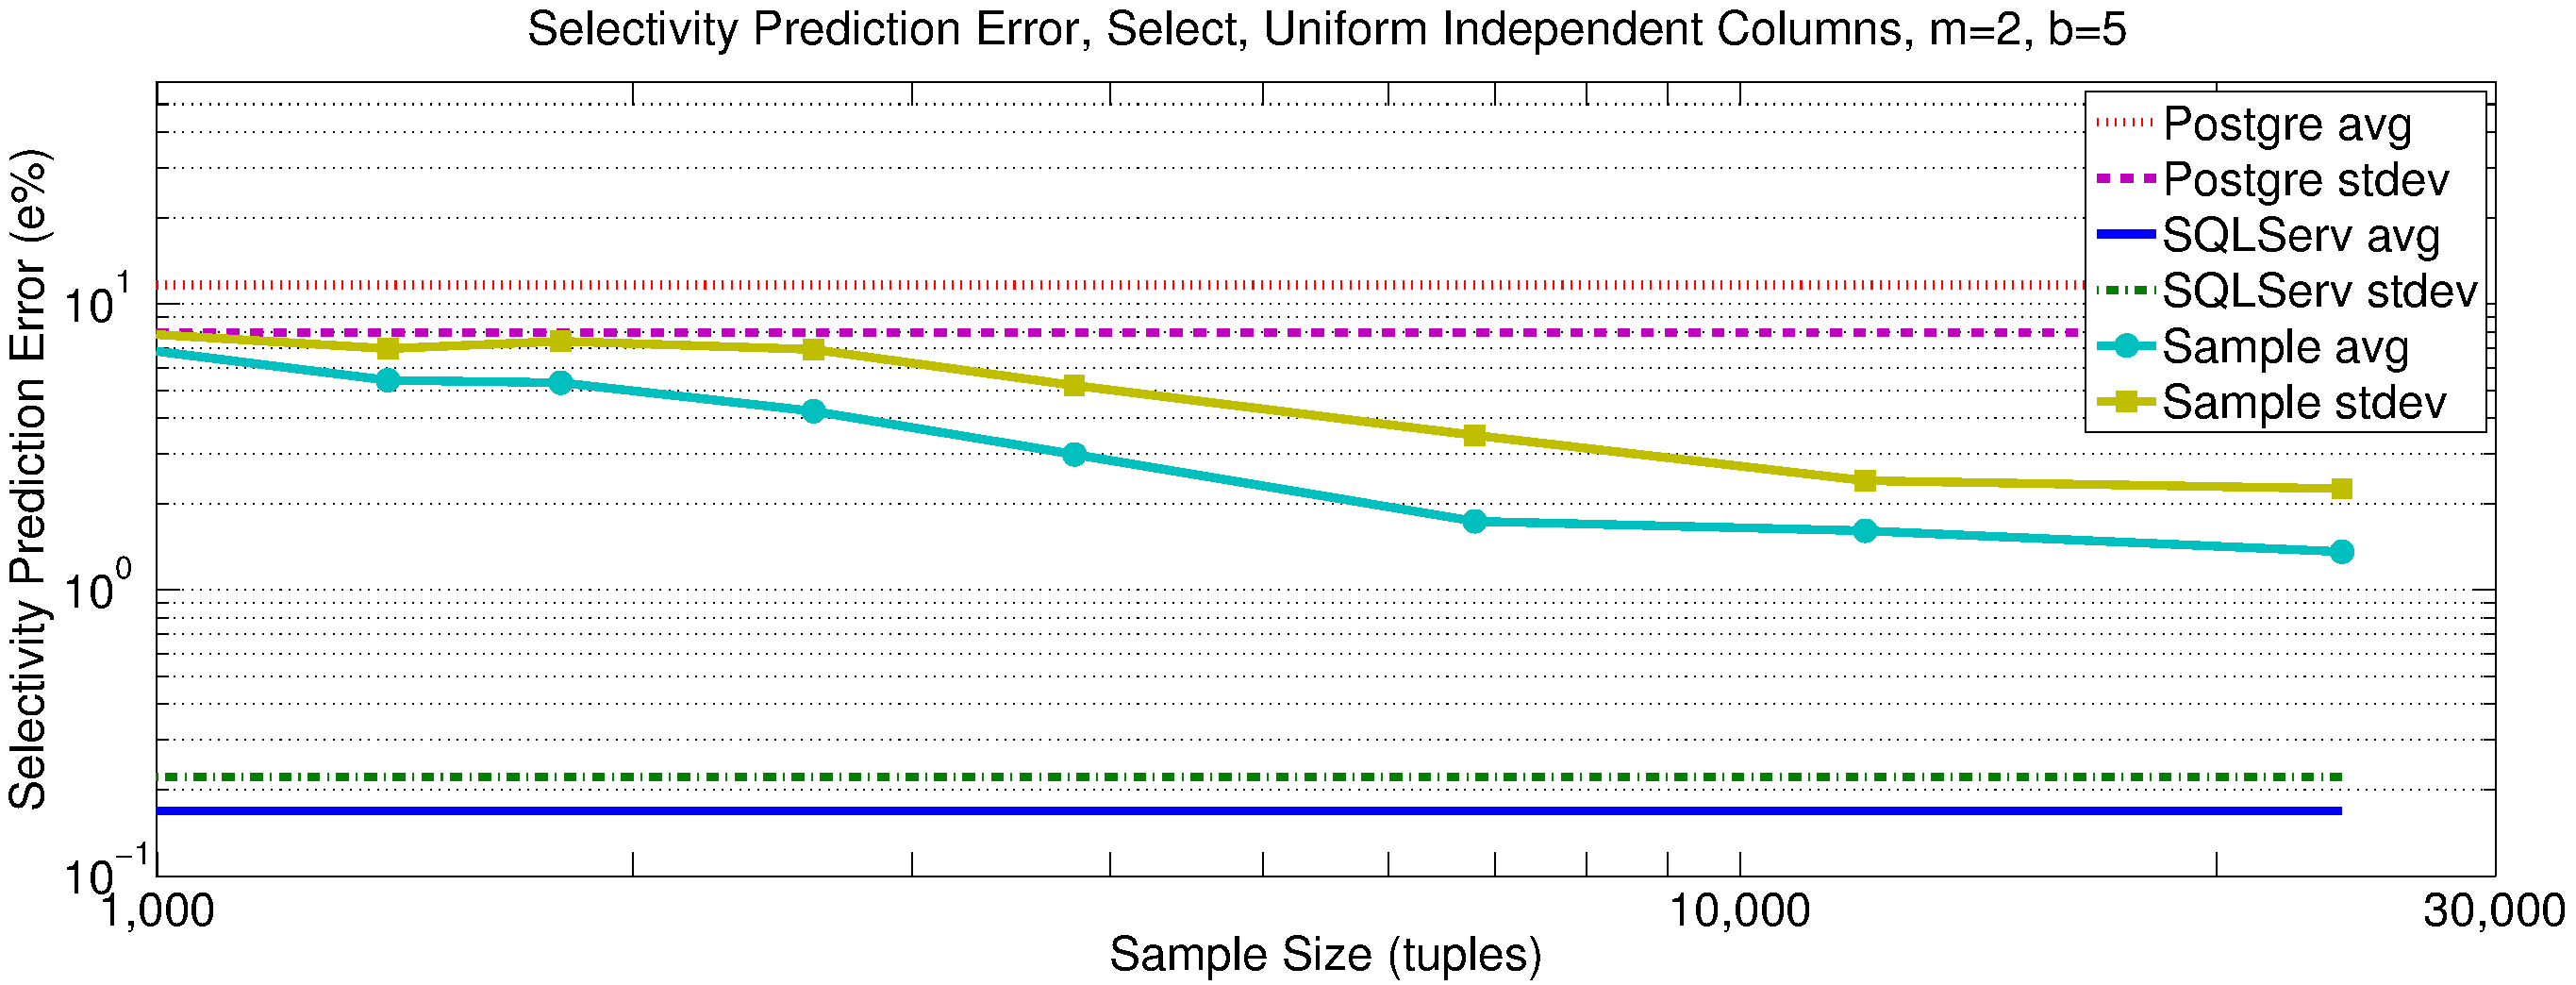
\includegraphics[scale=0.30]{vcfreq/T_k5_u200k_unif_k2_b5_errperc}
  %\vspace{-0.3cm}
  \caption{Selectivity prediction error for selection queries on a table with
  uniform independent columns -- Two columns ($m=2$), five Boolean clauses ($b=5$).}
  \label{fig:vcfreqT_k5_u200k_unif_k2_b5_errperc}
\end{figure}

Since the selectivity estimated by the our method was always within $\varepsilon$
from the actual, we report the actual percent error, i.e., the quantity
$e_\%=\frac{100|p(\sigma_q)-\sigma_\Db(q)|}{\sigma_\Db(q)}$ where $p(\sigma_q)$
is the predicted selectivity. We analyze the average and the standard deviation
of this quantity on a set of queries and the evolution of these measures as
the sample size increases. We can see from
Fig.~\ref{fig:vcfreqT_k5_u200k_unif_k2_b5_errperc}
%~\ref{fig:vcfreqT_k5_u200k_unif_k5_b5_errperc},
and~\ref{fig:vcfreqT_k2_correl_k2_b8_errperc} that both the average and the standard
deviation of the percentage error of the prediction obtained with our method
decrease as the sample size grows (the rightmost plotted
sample size is the one from Table~\ref{tab:samplesize}, i.e., the one computed 
in~Thm.\ref{thm:eapprox}. More interesting is the comparison in those figures between the performance of the
histograms and the performance of our techniques in predicting selectivities. When
the assumptions of the histograms hold, as is the case for the data plotted in
%Figures~\ref{fig:vcfreqT_k5_u200k_unif_k5_b5_errperc} and
Fig.~\ref{fig:vcfreqT_k5_u200k_unif_k2_b5_errperc}, the predictions obtained from the
histograms are good. 

\begin{figure}[htbp]
  \centering
  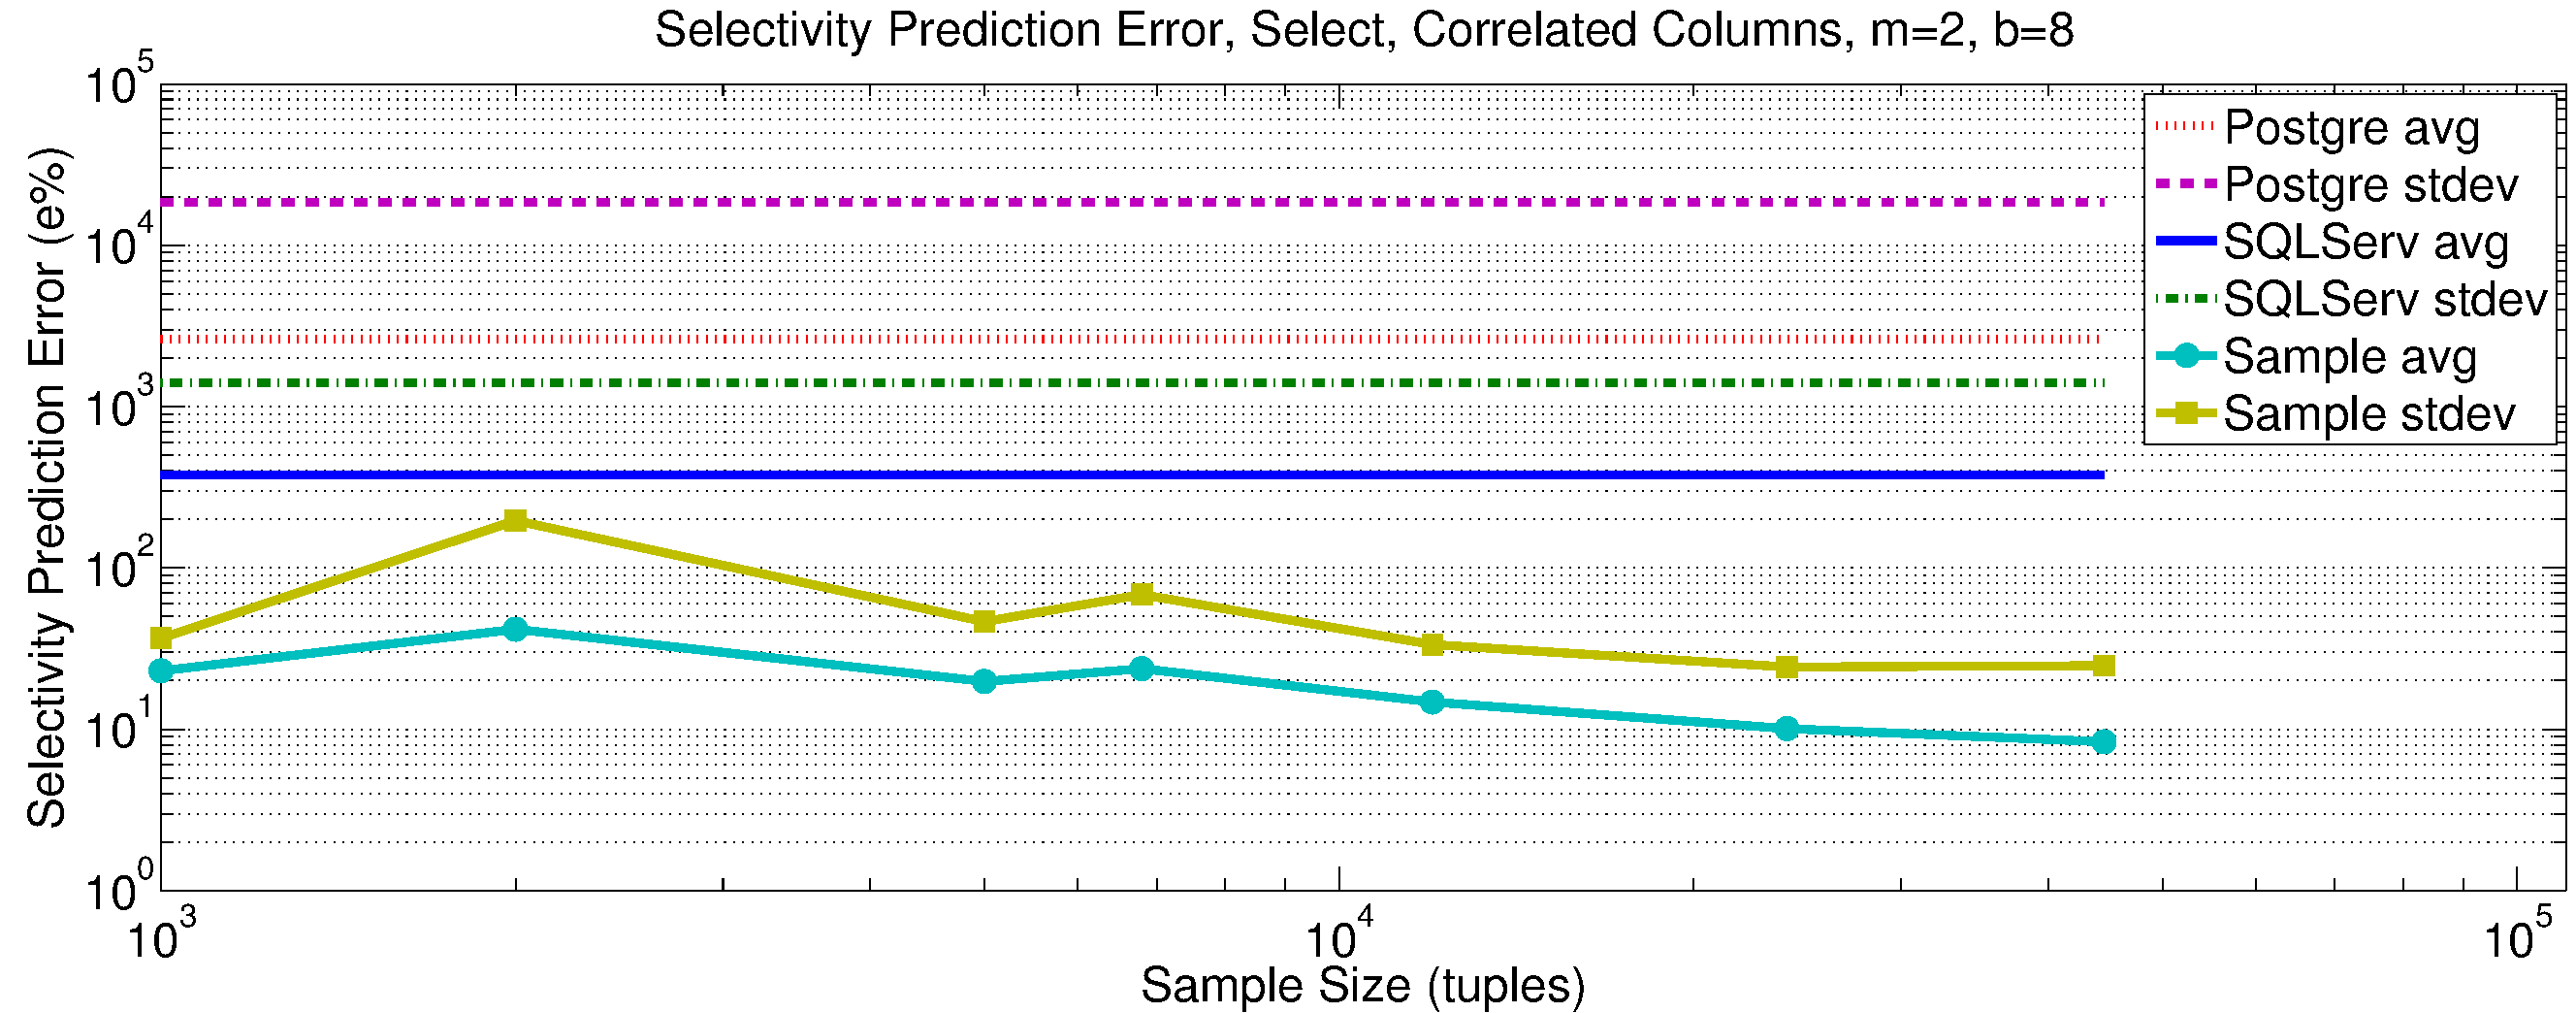
\includegraphics[scale=0.3]{vcfreq/T_k2_correl_k2_b8_errperc}
  %\vspace{-0.3cm}
  \caption{Selectivity prediction error for selection queries on a table with
  correlated columns -- Two columns ($m=2$), eight Boolean clauses ($b=8$).}
  \label{fig:vcfreqT_k2_correl_k2_b8_errperc}
\end{figure}

But as soon as the data are
correlated (Fig.~\ref{fig:vcfreqT_k2_correl_k2_b8_errperc}), our sampling method gives better
predictions than the histograms even at the smallest sample sizes and keeps
improving as the sample grows larger. It is also interesting to observe how the
standard deviation of the prediction error is much smaller for our method than
for the histograms, suggesting a much higher consistency in the quality of the
predictions. In Fig.~\ref{fig:vcfreqT_k2_correl_k2_b8_errperc} we do not show multiple
curves for the different PostgreSQL histograms because increasing the number of
buckets had very marginal impact on the quality of the estimates, sometimes even
in the negative sense (i.e., an histogram with more buckets gave worse
predictions than an histogram with fewer buckets), a fact that can be explained
with the variance introduced by the sampling process used to create the
histograms. For the same reason we do not plot multiple lines for the
prediction obtained from the multi-columns and single-column statistics of SQL
Server: even when the multi-column statistics were supposed to help, as in the
case of correlated data, the obtained prediction were not much different from
the ones obtained from the single-column histograms.

\paragraph{Join Queries.} The strength of our method compared to histograms is
even more evident when we run join queries, even when the histograms independent assumptions are
satisfied. In our experiments, the predictions obtained using our technique were
always within $\varepsilon$ from the real values, even at the smallest sample
sizes, but the same was not true for histograms. For example, in the case of
$m=1$ and $b=5$, $135$ out of $300$ predictions from the histograms were more
than $\varepsilon$ off from the real selectivities.
Figure~\ref{fig:vcfreqjoin_k1_b1_errperc} shows the comparison between the average and
the standard deviation of the percentage error, defined in the previous
paragraph, for the histograms and our method. The numbers include predictions
for the selection operations at the leaves of the query tree.

\begin{figure}[htbp]
  \centering
  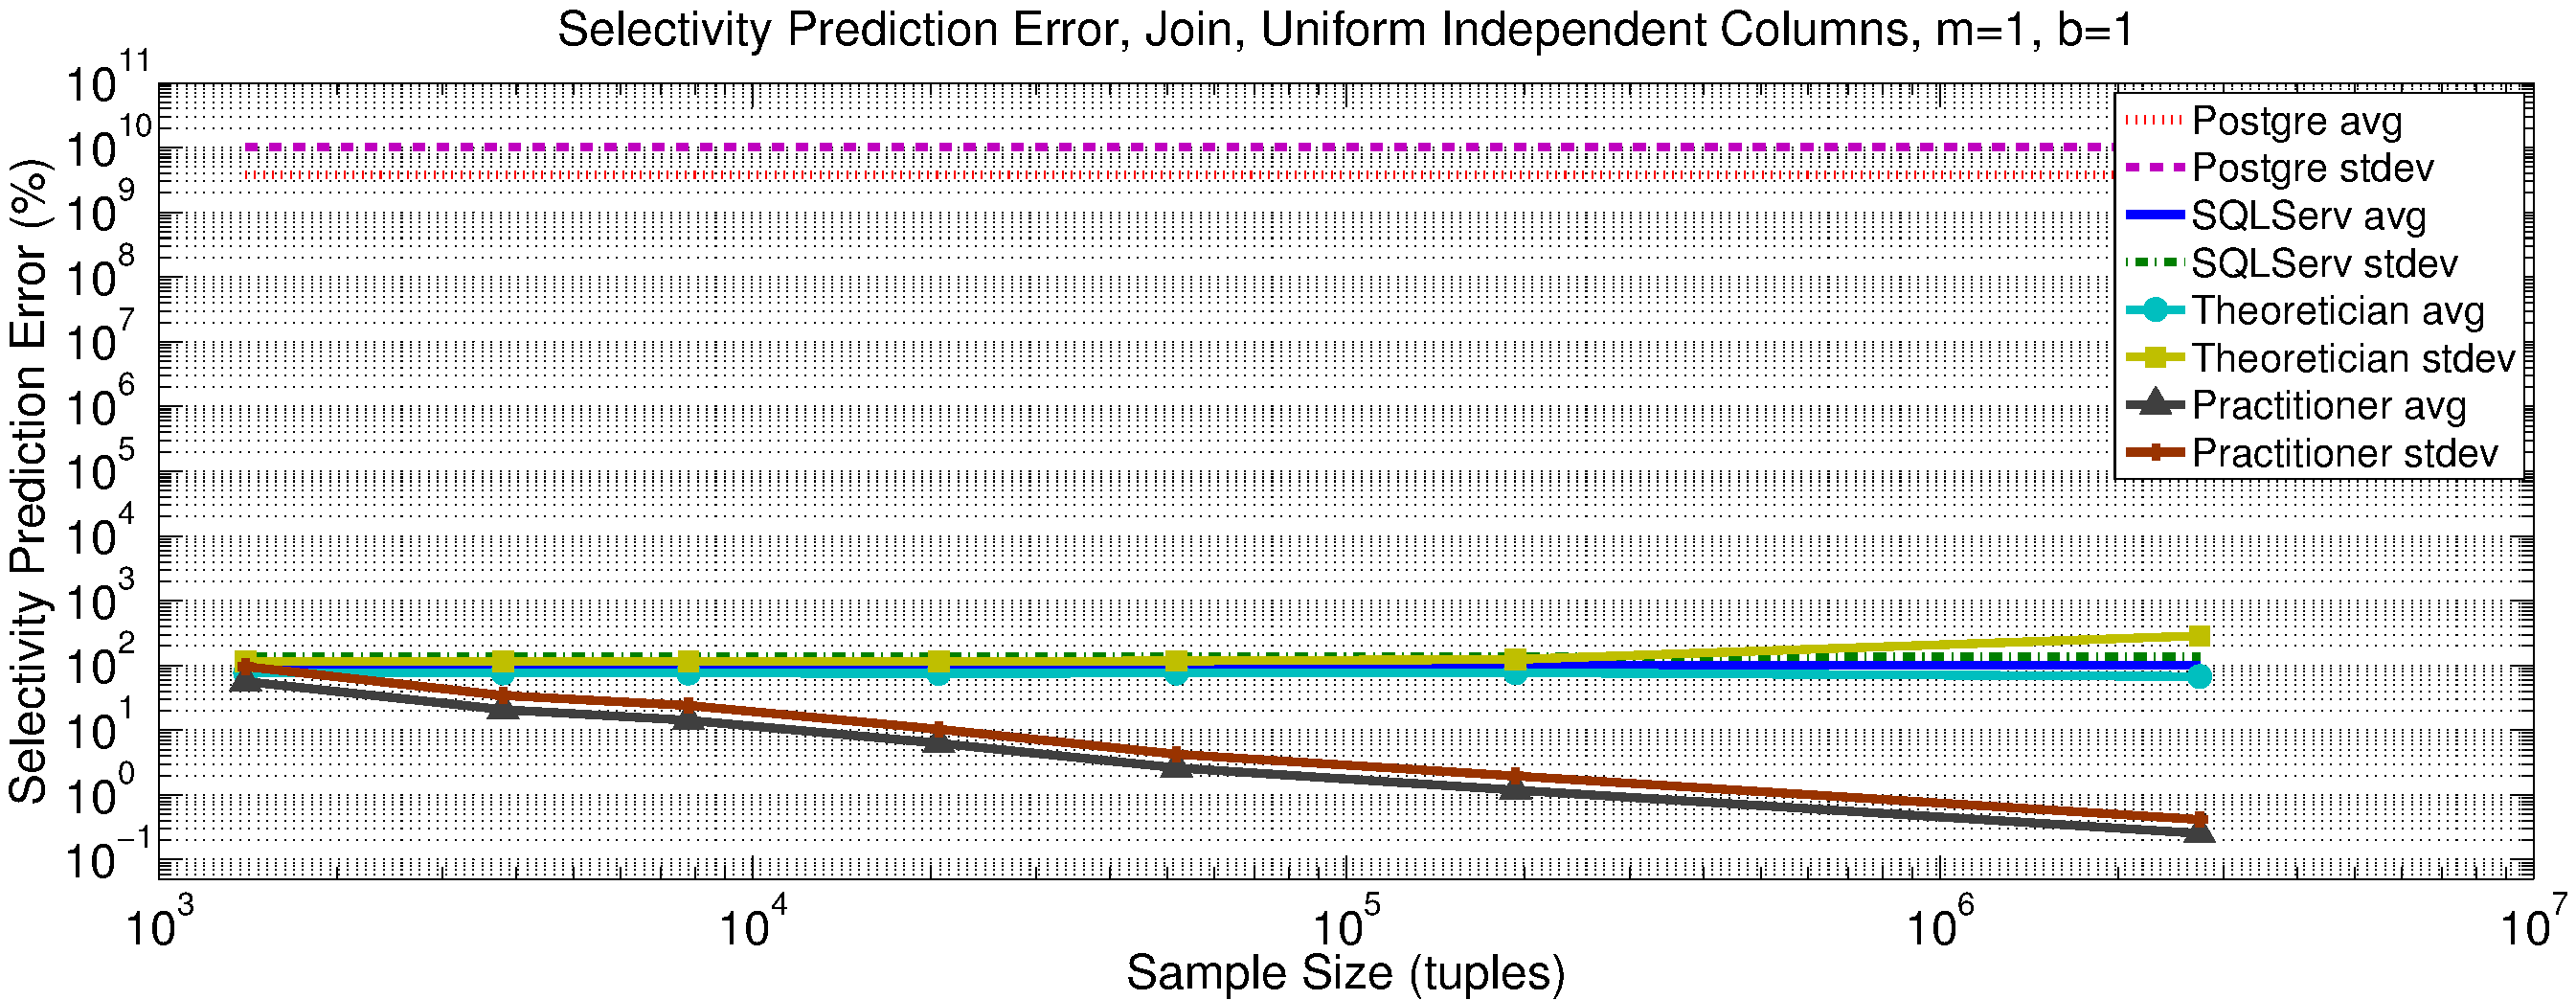
\includegraphics[scale=0.3]{vcfreq/join_k1_b1_errperc}
  %\vspace{-0.3cm}
  \caption{Selectivity prediction error for join queries queries. One column
  ($m=1$), one Boolean clause ($b=1$).}
  \label{fig:vcfreqjoin_k1_b1_errperc}
\end{figure}

Again,
we did not plot multiple curves for histograms with a different number of
buckets because the quality of the predictions did not improve as the histograms
became more fine-grained. To understand the big discrepancy between the accurate
predictions of our method and the wrong estimates computed by the histograms in
PostgreSQL  we note that  for some join queries, the
histograms predicted an output size on the order of the hundreds of thousands of
tuples but the actual output size was zero or a very small number of tuples.
Observing the curves of
the average and the standard deviation of the percentage error for the
prediction obtained with our method, we can see that at the smaller sample sizes
the quality of the predictions only improves minimally with the sample size.
This is due to the fact that at small sizes our prediction for the join
operation is very often zero or very close to zero, because the output of the
query does not contain enough pairs of tuples from the sample of the Cartesian
product of the input table (i.e., pairs of tuples with the same value in the
$sampleindex$ column). In these cases, the prediction can not be accurate at all
(i.e., the error is 100\% if the original output contained some tuples, or 0\% if
the query returned an empty set in the large databases). As soon as the sample
size grows more, we can see first a jump to higher values of the percentage
error, which then behaves as expected, i.e., decreasing as the sample size
increases. 

In Fig.~\ref{fig:vcfreqjoin_k1_b1_errperc} we also show a
comparison between the percentage error of predictions obtained using our method
in two different ways: the ``theoretically correct'' way that makes use of the
number of pairs of tuples with the same value in the $sampleindex$ column and
the ``practitioner'' way which uses the size of the output of the join operation
in the sample, therefore ignoring the $sampleindex$ column. Recall that we had
to add the $sampleindex$ column because Thm.~\ref{thm:eapprox} requires a
uniform sample of the Cartesian product of the input tables.
As it is evident from Fig.~\ref{fig:vcfreqjoin_k1_b1_errperc}, the ``practitioner''
way of predicting selectivity gives very good results at small sample sizes
(although it does not offer theoretical guarantees). These results are similar
in spirit, although not equivalent, to the theoretical conclusions presented
by~\citet{HaasNSS96} in the setting of selectivity estimation
using online sampling.

%\paragraph{Comments.} From the experiments we ran we can conclude that our
%method provides practically efficient and highly accurate technique for selectivity estimation. 
%The experiments also demonstrate that histograms, even when fine-grained and
%leveraged by the use of a MCV list, give poor estimates compared to our technique.
%The majoThe impossibility (by construction) to handle correlation in
%data makes them almost completely unsuitable for some real world applications
%requiring accurate selectivity estimates. It is also to be noted that, as the
%complexity of a query increases (in the sense of the number of operations
%involved) the more it is possible that the tuples at higher levels (towards the
%root) of the query plan become correlated, thus invalidating the histogram
%independence assumptions even if the base data are not correlated.  A comparison of the
%predictions obtained using our method and those obtained from a multidimensional
%histograms would be interesting to see how more ingenuous techniques may improve
%the usefulness of precomputed statistics. Nevertheless it is important to notice
%that in order to be able to take into account the possible correlations among
%all pairs of columns in a table, an histogram with an exponential (in the number
%of columns) number of dimension is needed, and it could still give low-quality
%selectivity predictions for queries whose complexity is greater than what the
%histogram could handle. Another interesting fact pointed out by our experiments
%is that a sample of the Cartesian product may not actually be needed, as the
%results in Fig.~\ref{fig:vcfreqjoin_k1_b1_errperc} shows, i.e., the bounds to the
%sample size may be such that a certain level of non-uniformity in the sampling
%process may be accommodated. It may even well be that the entire
%Thm.~\ref{thm:eapprox}, does not need the sample to be a uniform sample of the
%set of points.
%
\section{Conclusions}\label{sec:vcfreqcompar}
We develop a novel method for estimating the selectivity of queries by executing
it on a concise, properly selected, sample of the database. We present a
rigorous analysis of our method and extensive experimental results demonstrating
its efficiency and the accuracy of its predictions.

%As we discussed in Section~\ref{sec:vcfreqprevwork},
Most commercial databases use histograms built on a single column, for selectivity
estimation. There has also been significant research on improving the estimate
using multidimensional
histograms~\citep{BrunoCG01,PoosalaI97,SrivastavaHMKT,WangS03} and join
synopses~\citep{AcharyaGPR99}. The main advantage of our method is that it gives
uniformly accurate estimates for the selectivity of any query within a predefined
VC-dimension range. Methods that collect and store pre-computed statistics give
accurate estimates only for the relations captured by the collected statistics,
while estimate of any other relation relies on an independence assumption.
%, which give probabilistic guarantees on the error of the predicted
%selectivity,%
%Flexibility is one of the major aspects making our approach more suitable for
%practical implementation than the above advanced techniques (which, despite
%being presented some years ago, still have to be implemented in widespread
%DBMS). Once the parameters $m$, $b$, and $u$ for the class of queries to be run
%on the database have been fixed, the sample can be created and used to estimate
%the selectivities of the queries. From the way we defined our class of queries
%it should be clear that such a sample is able to give accurate estimation no
%matter what tables are joined together and no matter what the join columns in
%those table is. At the same time, the selectivity of any possible selection
%query in the class can be correctly estimated, independently of what columns
%appear in the selection predicate and how the different clauses composing the
%predicate are connected with Boolean operators. This make our approach extremely
%flexible.  
To match the accuracy of our new method with histograms and join synopses
one would need to create, for each table, a multidimensional histogram where the
number of dimensions is equal to the number of columns in the tables. The space
needed for a multidimensional histogram is exponential in the number of
dimensions, while the size of our sample representation is almost linear in that parameter. 
Furthermore, to estimate the selectivity for join operations
one would need to create join synopses for all pairs of columns in the database,
again in space that grows exponential in the number of columns.

VC-dimension, often considered only a theoretical tool, leads to an efficient
and practical tool for an important problem in database management.

%In the future, we will study the possibility of using results from the
%VC-dimension theory to solve the problem of computing good approximations of the
%results of aggregate functions applied to the outputs of database queries.


\chapter{Conclusions}\label{ch:conclusions}

The major goal of the work that led to this dissertation was to verify whether
VC-dimension could be used to develop practical sample size bounds for important
data analytics problems. Before this work, VC-dimension was considered of mostly
theoretical significance. We showed that it is possible to compute tight upper
bounds to the VC-dimension of relevant problems from different areas of data
analytics: knowledge discovery, graph analysis, and database management. 

The upper bounds are characteristic quantities of the dataset or of the
problem at hands. Not only they can be easy to compute, but they are usually
small in practice. This means that the sample size needed to obtain high quality
approximations of the results for the problem at hand may not need to depend on
the size of the dataset or on the number of patterns or ``questions'' that one
is interested to answer using the data. The sample sizes obtained using our
bounds are small and can fit into main memory, partially solving the issue of
analyzing very large datasets. Indeed, the practicality of our results is
exemplified by the fact that one of our algorithms (PARMA, see
Ch.~\ref{ch:parma}) was adapted and implemented to be used in
SAMOA~\citep{DFMorales13} at Yahoo (see also \url{http://yahoo.github.io/samoa/}).

Despite the many advantages of using VC-dimension when analyzing sample sizes
for randomized algorithms, one must not consider it a one-size-fits-all method
as its wide applicability may be hindered by the following factors:
\begin{itemize}
  \item{\bf Need for an efficient algorithm to compute bounds to the
    VC-dimension.} Bounding the VC-dimension of a problem is a challenging but
    good bounds can be found. Nevertheless, even if the bound is tight and it is a
    characteristic quantity of the dataset or of the problem at hand, actually
    computing this quantity may be computational expensive. We saw an example of
    this issue in Sect.~\ref{sec:centrsamplallvertapprox}, when dealing with the
    computation of the vertex-diameter of a directed or weighted graph. In that
    case, we were blessed by the presence of the logarithm in the bound of the
    VC-dimension, which allowed us to use a loose approximation of the vertex
    diameter, but this may not always be the case. Without a fast procedure to
    compute the upper bound to the VC-dimension (and therefore the needed sample
    size), the use of VC-dimension is severely limited.
  \item{\bf Need for an efficient sampling procedure.} A bound to the
    VC-dimension is not sufficient: the second necessary component is a sampling
    procedure to sample points of the domain according to the appropriate
    probability distribution. We described an example of how to develop such a
    sampling procedure in Sect.~\ref{sec:centrsamplallvertapprox}. It is of
    crucial importance that the sampling procedure is fast, otherwise many
    advantages of using sampling may be lost.
  \item{\bf Need of drawing independent samples.} In order to apply
    Thm.~\ref{thm:eapprox}, we need \emph{independent} samples from the
    distribution. At times, this may be a limitation. For example we saw in
    Sect.~\ref{sec:centrsampldiscussion} that the algorithm
    from~\citep{BrandesP07} draws multiple shortest paths at each step but they
    are dependent, as they all originate from the same vertex. By doing this,
    the algorithm collects more information, resulting in low variance in the
    estimation. Recent developments extends Thm.~\ref{thm:eapprox} to the case
    of ergodic sampling, therefore opening the possibility that the independence
    requirement may be relaxed~\citep{Catoni04,AdamsN11,AdamsN13,VanHandel13}.
  \item{\bf Dependency on $\varepsilon$.} If the probability mass of a range $R$ is
    smaller than $\varepsilon$, then a sample of size as suggested
    by~\eqref{eq:vceapprox} may not contain any point in $R$. This is especially annoying when a lot
    of ranges may have very small probability masses. In this case, a lower
    $\varepsilon$ should be used in order to compute acceptable approximations
    of these probability masses. The obvious drawback in using a lower
    $\varepsilon$ is that it directly corresponds to a larger sample. Given that
    the sample size depends on $1/\varepsilon^2$, the increase in the number of
    samples may be substantial for a small decrease in $\varepsilon$. A larger
    sample means a slower algorithm, and the advantages of using sampling may be
    lost or hindered. Before using Thm.~\ref{thm:eapprox} is therefore
    necessary to assess whether we are interested in good approximations of very
    small probability masses. If so, sampling may not be the best choice.
\end{itemize}

\section*{Future work} 
In this dissertation we studied the development and analysis of fast and
efficient algorithms for data analytics by taking into consideration different
aspects of the problem and different solutions. For each of these, there are a
number of possible directions for future research.

VC-dimension is one of many concepts from the broad field of statistical
learning theory. Other tools and results include data-dependent sample
complexity bounds based on Rademacher averages, pseudodimension, VC-shatter
coefficients, Bayesian uniform bounds, just to name a
few~\citep{BoucheronBL05,AnthonyB99,DevroyeGL96}. We showed that VC-dimension
can be have a practical impact to speed up algorithms for data analytics, but it
would be interesting to pursuit the use of these other concepts for the creation
of new algorithm or to further reduce the number of samples needed to
approximate. 

In this work we focused on ``one-shot'' sampling, i.e., the algorithms create a
single sample with size sufficient to obtain an approximation of desired
quality. \emph{Data-dependent bounds based on Rademacher averages} can be
useful to develop \emph{progressive sampling} algorithms that start from a small
sample size and check a stopping condition to understand whether they sampled
enough to obtain a good approximation~\citep{ElomaaK02,Kaariainen04}. The
challenge in creating such algorithms is in the development and analysis of a
stopping condition that can detect when to stop as soon as possible.  

A bound on the VC-dimension allows to estimate the expectation of 0-1 functions
using their empirical averages. \emph{Pseudodimension} instead works for
\emph{real-valued} functions. Since many datasets are real valued or can be seen
as collection of real valued functions (e.g., audio and video files and sensor
signals), investigating the use of pseudodimension to create sampling-based
randomized algorithms for data analytics problems on real data is an interesting
research direction.

One issue that we only partially tackle in Chapter~\ref{ch:realfis} is that of
\emph{statistical validation of the results}. We already explained in
Chapter~\ref{ch:intro} why only recently it started to receive attention in data
analytics\itodo{DO THIS!}. Although it is of primary importance to go beyond
simple multi-hypothesis testing corrections like the Union bound (a.k.a.~the
Bonferroni inequality) and we achieved it in Chapter~\ref{ch:realfis} for the
problem of frequent itemsets, there are other options to control false
positives. One example is controlling the False Discovery
Rate~\citep{BenjaminiH95} instead of the probability of having a false positive
(which is what we do in Chapter~\ref{ch:realfis} and is known as controlling the
Family-Wide Error Rate). There is huge room for improvement and the use of
VC-dimension to develop statistical tests to avoid the inclusion of false
positives in the results is only one possible directions. 

Research in the field of data analytics seems to have paid only limited
attention to recent developments in statistics and probability theory. We
believe that there may be room for improvements and significant contributions in
exploring the literature of these and other fields and adapt results and notions
that may have been considered only of theoretical interest to develop efficient
algorithm for practical problems involving the analysis of the ever-growing and
ever-changing amount of data available today.

In Chapter~\ref{ch:parma} we showed how it is possible to exploit the
power and scalability of modern computational platforms like MapReduce to create
algorithms for data analytics that can handle huge datasets that could not be
processed by a single machine. Technology is one of the driving forces behind
the development of new algorithms. It is important to leverage on the properties
of the next-generation of computational platforms and of hardware when
creating algorithms, in order to achieve the best performances. One particularly
interesting direction is the use of parallel/distributed platforms for data
streams. Algorithms for data streams have existed for a long time, but they
usually consider a single stream processed by a single machine. Platforms like
Spark\citep{ZahariaCFSS13} (see also \url{http://spark.incubator.apache.org/}),
where the stream is partitioned across multiple machines require new algorithms
that exploit their power. We implemented a streaming version of PARMA that was
integrated in Yahoo SAMOA~\citep{DFMorales13}. Adapting other MapReduce
algorithms to a distributed streaming setting or creating new algorithms for
such platforms is a challenging research direction.


\bibliographystyle{plainnat}
\bibliography{biblio/fimine,biblio/graphmine,biblio/mr,biblio/mrfim,biblio/riondapubs,biblio/sperner,biblio/statisticaltesting,biblio/statsigfis,biblio/various,biblio/vcfreq,biblio/vcmine,biblio/vcgraph,biblio/bidirectionalsearch,biblio/centrality,biblio/diamapprox}
\end{document}

